%% monografia.tex, fabiokepler, jeancheiran
%% Copyright 2012-2018 by UNIPAMPA LaTeX group at https://bitbucket.org/unipampaalegrete/monografias-cc-es-repo/
%%
%% This work may be distributed and/or modified under the conditions of the LaTeX Project Public
%% License, either version 1.3 of this license or (at your option) any later version.
%% The latest version of this license is in
%%   http://www.latex-project.org/lppl.txt
%% and version 1.3 or later is part of all distributions of LaTeX version 2005/12/01 or later.
%%
%% Based on the example file abtex2-modelo-trabalho-academico.tex of the abntex2 package
%% (http://abntex2.googlecode.com/) and on the ppgccufmg 1.45beta2 class
%% (http://vilarneto.com/ppgccufmg,
%% http://www.dcc.ufmg.br/pos/alunos/modelodisstese.php
%% and http://www.dcc.ufmg.br/~mirella).
%%
%% Adapted for the Computer Science program at UNIPAMPA (http://www.unipampa.edu.br)
%% by Fabio Kepler (fabio@kepler.pro.br) and Jean Cheiran (jeancheiran@unipampa.edu.br).
%%
%% Version 2.5 - 2018/08
%% Version 2.4 - 2017/05
%% Version 2.3 - 2013/03

% +++++++++++++++++++++++++++++++++++++++++++++++++++++++++++++++++++++++++++++++++++++++++++++++++
% Este modelo utiliza o pacote abnTeX2. Veja como instalá-lo em seu ambiente em
% http://abntex2.googlecode.com/.
% -------------------------------------------------------------------------------------------------
% abnTeX2: Modelo de Trabalho Acadêmico (tese de doutorado, dissertação de
% mestrado e trabalhos monográficos em geral) em conformidade com
% ABNT NBR 14724:2011: Informação e documentação - Trabalhos acadêmicos -
% Apresentação
% -------------------------------------------------------------------------------------------------
% Normas institucionais utilizadas:
% http://porteiras.r.unipampa.edu.br/portais/sisbi/programa-de-capacitacao/
% +++++++++++++++++++++++++++++++++++++++++++++++++++++++++++++++++++++++++++++++++++++++++++++++++

\documentclass[12pt,openright,twoside,a4paper,english,chapter=TITLE]{abntex2}    % frente e verso
%\documentclass[12pt,oneside,a4paper]{abntex2}            % apenas frente

% +++++++++++++++++++++++++++++++++++++++++++++++++++++++++++++++++++++++++++++++++++++++++++++++++
% PACOTES
% -------------------------------------------------------------------------------------------------

\usepackage{url}
\usepackage{amsmath,amssymb,amsfonts}
\usepackage{algorithmic}
\usepackage{graphicx}
\usepackage{textcomp}
% \usepackage{xcolor}
\usepackage{color}
\usepackage{booktabs}
\usepackage{colortbl}
\usepackage{balance}
\usepackage[english]{cleveref}
\usepackage{threeparttable}
\pagestyle{plain}
\usepackage{pdflscape}

% \usepackage{microtype}
\usepackage{lipsum}				% para geração de dummy text

% \usepackage{paralist} %inparaenum, conflita com enumitem
\usepackage[x11names,dvipsnames,table]{xcolor}

\usepackage{adjustbox}
\usepackage{todonotes}
\usepackage{hyperref} 
\usepackage{array}
\usepackage{booktabs}
\usepackage{colortbl}
\usepackage{longtable}
\usepackage{multirow}
\usepackage[outline]{contour}
\contourlength{1pt}
\usetikzlibrary{patterns}
%\rowcolors{1}{gray!10}{}
\usepackage{smartdiagram}

\usepackage{textcomp} % sinal de grau

\usepackage{amssymb}

\usepackage{listings}

\usepackage{pgf-pie}

\smartdiagramset{circular distance=3.5cm, font=\medium, text width=2.0cm,
module minimum width=1.5cm, module minimum height=1.0cm,arrow tip=to,uniform connection color=true,uniform color list=blue!30 for 7 items}

\def\BibTeX{{\rm B\kern-.05em{\sc i\kern-.025em b}\kern-.08em
    T\kern-.1667em\lower.7ex\hbox{E}\kern-.125emX}}

%PGPLOTS
\usepackage{pgfplots}
\usetikzlibrary{patterns}
\usepgfplotslibrary[statistics] % ConTEXt
\usetikzlibrary{pgfplots.statistics} % LATEX and plain TEX
\usepackage{tikz}
\usepackage{ragged2e}

\usetikzlibrary{patterns}
%\rowcolors{1}{gray!10}{}

\usetikzlibrary{angles,shadows,positioning,backgrounds,mindmap}

\pgfplotsset{width=9cm, height=8cm, compat=1.9}

\usetikzlibrary{shapes,backgrounds}
\def\BibTeX{{\rm B\kern-.05em{\sc i\kern-.025em b}\kern-.08em
    T\kern-.1667em\lower.7ex\hbox{E}\kern-.125emX}}

% começo da bagunça
\usetikzlibrary{angles,shadows.blur,positioning,backgrounds}
\usepackage{forest}
\forestset{
  declare count register=disjuncts from,
  disjuncts from'=0,
  declare count register=concrete from,
  concrete from'=2,
  concrete colour/.code={\colorlet{concretecol}{#1}},
  abstract colour/.code={\colorlet{abstractcol}{#1}},
  draw colour/.code={\colorlet{drawcol}{#1}},
  concrete colour=gray,
  abstract colour=white,
  draw colour=black,
  /tikz/mandatory/.style={circle, fill=drawcol, draw=drawcol},
  /tikz/optional/.style={circle, draw=drawcol, fill=white},
  /tikz/concrete/.style={fill=concretecol, draw=drawcol},
  /tikz/abstract/.style={fill=abstractcol, draw=drawcol},
  /tikz/or/.style={},
  mandatory/.style={edge label={node [mandatory] {}}},
  optional/.style={edge label={node [optional] {}}},
  or/.style={for first={disjunct}},
  disjunct/.style={
    tikz+={\path (.parent) coordinate (A) -- (!u.children) coordinate (B) -- (!ul.parent) coordinate (C) pic [fill=drawcol] {angle};}
  },
  disjunction tree/.style={
    where={isodd(n_children())}{
      for n={int((n_children()+1)/2)}{calign with current},
    }{
      calign=midpoint,
    },
    before typesetting nodes={
      for nodewalk={
        filter/.wrap pgfmath arg={{level>=##1}{n_children()>1}}{(disjuncts_from)}
      }{
        or,
      },
      where={level()>=(concrete_from)}{
        concrete,
      }{
        abstract,
      },
      tikz+={
        [font=\sffamily]
        \node (l) [anchor=north east, xshift=10pt] at (current bounding box.north east) {Legend};
        \foreach \i/\j [remember=\i as \k (initially l)] in {mandatory/Mandatory,optional/Optional,or/Or,abstract/Abstract,concrete/Concrete}
        {
          \node (\i) [below=20pt of \k.north, anchor=north, text centered, \i, minimum width=5pt,] {};
          \node (\j) [right=15pt of \i.center -| mandatory.west, anchor=west] {\j};
        };
        \draw [drawcol] (or.south west) coordinate (A) -- (or.north) coordinate (B) -- (or.south east) coordinate (C) pic [fill=drawcol, angle radius=5pt] {angle};
        \foreach \i in {mandatory,optional} \draw [darkgray] (\i.north east) -- +(45:5pt);
        \node (c) [below=0pt of Concrete.south] {};
        \scoped[on background layer]{\node [draw, fill=white, blur shadow, fit=(l) (Mandatory) (Optional) (Or) (Abstract) (Concrete) (c), rounded corners] {};}
      },
    },
    for tree={
      parent anchor=children,
      child anchor=parent,
      l'+=10mm,
      blur shadow,
      rounded corners,
      text height=2ex,
      text depth=.5ex,
      font=\sffamily,
    }
    % qtree/.style={
    %     for tree={
    %         parent anchor=south, 
    %         child anchor=north,
    %         align=center,
    %         inner sep=0pt,
    %         l'+=10mm,
    %         blur shadow,
    %         rounded corners,
    %         text height=2ex,
    %         text depth=.5ex,
    %         font=\sffamily,
    %     }
    % },
  },
}

%\pagestyle{plain} %Shows page number

% fim da bagunça


\usepackage{amssymb,enumitem}
% Pacotes fundamentais
\usepackage{cmap}           % Mapeamento de caracteres especiais no PDF
\usepackage{lmodern}        % Usa fonte Latin Modern
\usepackage[T1]{fontenc}    % Seleção de codificação de fonte
\usepackage[utf8]{inputenc} % Codificação do arquivo (conversão automática dos acentos)
% \usepackage[english]{babel}
% \usepackage[brazil]{babel}  % Idioma para hifenização e tradução de vários elementos
\usepackage{makeidx}        % Criação de índice
\usepackage{hyperref}       % Formatação do índice
\usepackage{lastpage}       % Usado pela Ficha catalográfica
\usepackage{indentfirst}    % Indenta o primeiro parágrafo de cada seção
%\usepackage[usenames,dvipsnames]{xcolor}  % Controle das cores (com nomes)
%\usepackage{graphicx}       % Inclusão de gráficos
\usepackage{booktabs}       % Formatação de tabelas
\usepackage{caption}
\usepackage{subcaption}
\usepackage{svg}            % incluir imagens SVG

% -------------------------------------------------------------------------------------------------
% Para citações
\usepackage[english,hyperpageref]{backref} % Páginas com as citações na bibliografia
\usepackage[alf,abnt-emphasize=bf, language = english]{abntex2cite} % Citações padrão ABNT (alfanumérico)
% \usepackage[backend=biber, style=abnt, ittitles]{biblatex}


% -------------------------------------------------------------------------------------------------
% Pacotes opcionais
\usepackage{nomencl}        % Para criar uma lista de símbolos
\usepackage{acro}           % Para usar acrônimos e abreviaturas
\usepackage{tikz}           % Para fazer figuras, diagramas e gráficos integrados e elegantes
\usepackage{pgfplots}       % Usa o pacote tikz para fazer gráficos muito melhores que os do Excel
\usepackage{pgfplotstable}  % Para gerar tabelas automaticamente a partir de arquivos com dados
\usepackage{filecontents}   % Para colocar o conteúdo de um arquivo dentro de um arquivo tex
\usepackage{todonotes}      % Para criar anotações durante o desenvolvimento do texto
%\usepackage{multirow}       % Permite fazer tabelas com múltiplas linhas
%\let\newfloat=\undefined    % Workaround para usar o pacote algorithm
%\usepackage{algorithm}      % Para escrever algoritmos
%\usepackage{clrscode}       % Para escrever algoritmos
%\usepackage{clrscode3e}     % Para escrever algoritmos; mais simples que os pacotes acima
\usepackage{pdfpages}        % Para incluir a folha de aprovação assinada em PDF
% -------------------------------------------------------------------------------------------------
% Configurações de pacotes
% -------------------------------------------------------------------------------------------------
\addto\captionsbrazil{
  \renewcommand{\listfigurename}{List of Figures}
}
% -------------------------------------------------------------------------------------------------
% Configurações do pacote backref
% Usado sem a opção hyperpageref de backref
\renewcommand{\backrefpagesname}{Cited at page(s):~}
% Texto padrão antes do número das páginas
\renewcommand{\backref}{}
% Define os textos da citação
\renewcommand*{\backrefalt}[4]{
    \ifcase #1 %
        No cited on text.%
    \or
        Cited at page #2.%
    \else
        Cited #1 times at pages #2.%
    \fi}%
% -------------------------------------------------------------------------------------------------
% Configurações de aparência do PDF final
%\definecolor{blue}{RGB}{41,5,195}
% \definecolor{webgreen}{rgb}{0,.5,0}
% Metainformações do PDF e cores dos links
\hypersetup{
  english,
  %backref=true,
  %pagebackref=true,
  %bookmarks=true,             % show bookmarks bar?
  %bookmarksnumbered=true,
  bookmarksdepth=4,
  pdftitle={\@title},
  pdfauthor={\@author},
  pdfsubject={\imprimirpreambulo},
  pdfkeywords={UNIPAMPA}{Software Engineering}{UNIPAMPA}{abntex}{TCC},
  %pdfproducer={LaTeX with abnTeX2},     % producer of the document
  pdfcreator={\@author},
  colorlinks=true,           % false: boxed links; true: colored links
  linkcolor=blue,            % color of internal links
  citecolor=blue,            % color of links to bibliography
  filecolor=black,         % color of file links
  urlcolor=black
}
%   linktocpage,
%   colorlinks,
%   citecolor=webgreen,
%   urlcolor=Maroon,
%   linkcolor=RoyalBlue,
%   filecolor=black,
% -------------------------------------------------------------------------------------------------
% Espaçamentos entre linhas e parágrafos
% O tamanho do parágrafo é dado por
\setlength{\parindent}{1.3cm}
% Controle do espaçamento entre um parágrafo e outro
\setlength{\parskip}{0.2cm} % tente também \onelineskip
% Controles do espaçamento entre linhas
%\OnehalfSpacing       % espaçamento um e meio (padrão);
%\DoubleSpacing        % espaçamento duplo
%\SingleSpacing        % espaçamento simples
% -------------------------------------------------------------------------------------
% Para o pacote de acrônimos
\acsetup{hyperref=true,index=true} %first-style=short}
% -------------------------------------------------------------------------------------
% Para o pacote tikz, pgfplots e pgfplotstable
\usetikzlibrary{arrows,chains,matrix,positioning,decorations.pathreplacing,calc}
% -------------------------------------------------------------------------------------
% Para poder usar subfiguras e subtabelas
\newsubfloat{figure}
\newsubfloat{table}
\providecommand*{\subfigureautorefname}{\figureautorefname}
% +++++++++++++++++++++++++++++++++++++++++++++++++++++++++++++++++++++++++++++++++++++


% +++++++++++++++++++++++++++++++++++++++++++++++++++++++++++++++++++++++++++++++++++++
% Informações de dados para CAPA e FOLHA DE ROSTO
% -------------------------------------------------------------------------------------

\titulo{ERtext: a text-based approach for designing and conceptual modeling relational databases}
\autor{Jonnathan Riquelmo Lopes Frescura}
\local{Alegrete}
\data{2022}
\orientador{Prof. PhD. Maicon Bernardino da Silveira}
\coorientador{Prof. PhD. Fábio Paulo Basso}
% \instituicao{Federal University of Pampa}
\instituicao{UNIVERSIDADE FEDERAL DO PAMPA}
%\tipotrabalho{Projeto de Trabalho de Conclusão de Curso~} % Para TCC I
%\tipotrabalho{Master Thesis~} % Para TCC II
\tipotrabalho{Master's Qualification Exam~}
% O preambulo deve conter o tipo do trabalho, o objetivo, o nome da instituição e a área de concentração
\preambulo{\imprimirtipotrabalho presented as partial requirement for obtaining the degree of Masters of Software Engineering at Federal University of Pampa (Unipampa).}
% +++++++++++++++++++++++++++++++++++++++++++++++++++++++++++++++++++++++++++++++++++++

% -------------------------------------------------------------------------------------
% Compila o indice
\makeindex
% Compila a lista de abreviaturas e siglas
% Para funcionar, o seguinte comando deve ser executado:
% makeindex ARQUIVO_PRINCIPAL.nlo -s nomencl.ist -o ARQUIVO_PRINCIPAL.nls
\makenomenclature
% -------------------------------------------------------------------------------------

% -------------------------------------------------------------------------------------
% Abreviaturas (definido pelo parâmetro 'class')
\DeclareAcronym{fig}{
  short = Fig.,
  long  = Figure,
  class = abreviaturas
}
% -------------------------------------------------------------------------------------
% Acrônimos/Siglas (definido pelo parâmetro 'class')
\DeclareAcronym{tcc}{
  short = TCC,
  long  = Trabalho de Conclusão de Curso,
  long-plural-form = Trabalhos de Conclusão de Curso,
  class = acronimos
}

\DeclareAcronym{db}{
  short = DB,
  long  = Database,
  long-plural-form = databases,
  class = acronimos
}

\DeclareAcronym{dbms}{
  short = DBMS,
  long  = Database Management System,
  long-plural-form = Database Management Systems,
  class = acronimos
}

\DeclareAcronym{dsl}{
  short = DSL,
  long  = Domain-Specific Language,
  long-plural-form = Domain-Specific Languages,
  class = acronimos
}

\DeclareAcronym{sql}{
  short = SQL,
  long  = Structured Query Language,
  long-plural-form = Structured Query Languages,
  class = acronimos
}

\DeclareAcronym{mde}{
  short = MDE,
  long  = Model-Driven Engineering,
  class = acronimos
}

\DeclareAcronym{mdse}{
  short = MDSE,
  long  = Model-Driven Software Engineering,
  class = acronimos
}

\DeclareAcronym{mdd}{
  short = MDD,
  long  = Model-Driven Development,
  class = acronimos
}

\DeclareAcronym{mda}{
  short = MDA,
  long  = Model-Driven Architecture,
  class = acronimos
}

\DeclareAcronym{omg}{
  short = OMG,
  long  =  \textit{Object Management Group},
  class = acronimos
}

\DeclareAcronym{cim}{
  short = CIM,
  long  =  Computation-Independent Model,
  class = acronimos
}

\DeclareAcronym{pim}{
  short = PIM,
  long  =  Plataform-Independent Model,
  class = acronimos
}

\DeclareAcronym{psm}{
  short = CIM,
  long  =  Plataform-Specific Model,
  class = acronimos
}

\DeclareAcronym{case}{
  short = CASE,
  long  =  Computer-Aided Software Engineering,
  class = acronimos
}

\DeclareAcronym{css}{
  short = CSS,
  long  = Cascading Style Sheets,
  class = acronimos
}

\DeclareAcronym{sysml}{
  short = SysML,
  long  = Systems Modeling Language,
  class = acronimos
}
\DeclareAcronym{vhdl}{
  short = VHDL,
  long  = VHSIC Hardware Description Language,
  class = acronimos
}
\DeclareAcronym{uml}{
  short = UML,
  long  =  Unified Modeling Language,
  long-plural-form =  Unified Modeling Language,
  class = acronimos
}
\DeclareAcronym{xml}{
  short = XML,
  long  = eXtensible Markup Language,
  class = acronimos
}
\DeclareAcronym{html}{
  short = HTML,
  long  =  HyperText Markup Language,
  class = acronimos
}
\DeclareAcronym{lw}{
  short = LW,
  long  = Language Workbench,
  long-plural-form =  Language Workbenches,
  class = acronimos
}

\DeclareAcronym{ide}{
  short = IDE,
  long  =  Integrated Development Environment,
  long-plural-form = Integrated Development Environments,
  class = acronimos
}
\DeclareAcronym{rcp}{
  short = RCP,
  long  =  Rich Client Platform,
  long-plural-form = Rich Client Platforms,
  class = acronimos
}
\DeclareAcronym{emf}{
  short = EMF,
  long  =  Eclipse Modeling Framework,
  class = acronimos
}
\DeclareAcronym{ast}{
  short = AST,
  long  =  Abstract Syntax Tree,
  class = acronimos
}
\DeclareAcronym{dom}{
  short = DOM,
  long  =  Document Object Graph,
  class = acronimos
}
\DeclareAcronym{bnf}{
  short = BNF,
  long  = Backus-Naur Form,
  class = acronimos
}
\DeclareAcronym{ebnf}{
  short = EBNF,
  long  = Extended Backus-Naur Form,
  class = acronimos
}

\DeclareAcronym{gpl}{
  short = GPL,
  long  = General-Purpose Programming Language,
  long-plural-form = General-Purpose Programming Languages,
  class = acronimos
}

\DeclareAcronym{er}{
  short = ER,
  long  = Entity-Relationship,
  class = acronimos
}

\DeclareAcronym{ddl}{
  short = DDL,
  long  = Data Definition Language,
  long-plural-form = Data Definition Languages,
  class = acronimos
}

\DeclareAcronym{dml}{
  short = DML,
  long  = Data Manipulation Language,
  long-plural-form = Data Manipulation Languages,
  class = acronimos
}

\DeclareAcronym{ex1}{
  short = EX1,
  long  = Experiment 1,
  class = acronimos
}

\DeclareAcronym{ex2}{
  short = EX2,
  long  = Experiment 2,
  class = acronimos
}

\DeclareAcronym{ex3}{
  short = EX3,
  long  = Experiment 3,
  class = acronimos
}

\DeclareAcronym{sus}{
  short = SUS,
  long  = System Usability Scale,
  class = acronimos
}

\DeclareAcronym{rte}{
  short = RTE,
  long  = Round-trip Engineering,
  class = acronimos
}

\DeclareAcronym{orm}{
  short = ORM,
  long  = Object-relational Mapping,
  class = acronimos
}


% -------------------------------------------------------------------------------------------------
% Nomenclaturas/Símbolos
%\nomenclature{$A_i$}{Área do $i^{esimo}$ componente}
%\nomenclature{456}{Isto é um número}
%\nomenclature{123}{Isto é outro número}
%\nomenclature{$n$}{Tamanho da entrada}
%\nomenclature{$V$}{Vetor de elementos}
%\nomenclature{$\mathcal{T}$}{Conjunto de trabalhos de TCC}

% -------------------------------------------------------------------------------------------------
% Inclui alguns ajustes finos para que fique de acordo com o Manual de Normatização
% Pequenos consertos e ajustes para que fique de acordo com o Manual de Normatização 2011.

\setlength{\ABNTEXsignwidth}{12cm}

% ---
% Impressão da Capa
\renewcommand{\imprimircapa}{%
  \begin{capa}%
    \center
    {\ABNTEXchapterfont\large\MakeUppercase\imprimirinstituicao}

    \vspace*{\fill}
    {\ABNTEXchapterfont\large\imprimirautor}

    \vspace*{\fill}
    {\ABNTEXchapterfont\bfseries\LARGE\imprimirtitulo}

    \vspace*{\fill}
    ~
    \vspace*{\fill}

    {\large\imprimirlocal}
    \par
    {\large\imprimirdata}

    \vspace*{1cm}
  \end{capa}
}
% ---


% ---
% Impressão da Folha de Rosto
\makeatletter
\renewcommand{\folhaderostocontent}{
  \begin{center}

    {\ABNTEXchapterfont\large\imprimirautor}

    \vspace*{\fill}%\vspace*{\fill}
    {\ABNTEXchapterfont\bfseries\Large\imprimirtitulo}
    \vspace*{\fill}

    \abntex@ifnotempty{\imprimirpreambulo}{%
      \hspace{.45\textwidth}
      \begin{minipage}{.5\textwidth}
        {\SingleSpacing
        \imprimirpreambulo}

        \vspace*{1em}
        \imprimirorientadorRotulo~\imprimirorientador\par

        \abntex@ifnotempty{\imprimircoorientador}{%
          \vspace*{1em}
          \imprimircoorientadorRotulo~\imprimircoorientador%
        }%

      \end{minipage}%
      \vspace*{\fill}
    }%

    {\large\imprimirlocal}
    \par
    {\large\imprimirdata}
    \vspace*{1cm}

  \end{center}
}
\makeatother
% ---

% ---
\renewcommand{\ABNTEXchapterfont}{\rmfamily\bfseries}
\setsecheadstyle{\rmfamily\bfseries}

\renewcommand{\ABNTEXchapterfontsize}{\normalsize}
\renewcommand{\ABNTEXsectionfontsize}{\normalsize}
\renewcommand{\ABNTEXsubsectionfontsize}{\normalsize}
\renewcommand{\ABNTEXsubsubsectionfontsize}{\normalsize}
\renewcommand{\ABNTEXsubsubsubsectionfontsize}{\normalsize}

% Espaçamento entre título e texto
\setlength\afterchapskip{\lineskip}

% Espaçamento entre parágrafos
\setlength{\parskip}{0.cm}

% ---




% *************************************************************************************************
\begin{document}
\selectlanguage{english}
% *************************************************************************************************

% +++++++++++++++++++++++++++++++++++++++++++++++++++++++++++++++++++++++++++++++++++++++++++++++++
% ELEMENTOS PRÉ-TEXTUAIS
% +++++++++++++++++++++++++++++++++++++++++++++++++++++++++++++++++++++++++++++++++++++++++++++++++
% \pretextual

% -----------------------------------------------
% Capa [OBRIGATÓRIO]
% -----------------------------------------------
\imprimircapa

% -----------------------------------------------
% Folha de rosto [OBRIGATÓRIO]
% -----------------------------------------------
% (ver documentação do abntex2 caso seja necessário haver ficha catalográfica)
\imprimirfolhaderosto

% -----------------------------------------------
% Folha de aprovação [OBRIGATÓRIO]
% -----------------------------------------------
% Veja alguns detalhes no arquivo.
% -----------------------------------------------
% Folha de aprovação [OBRIGATÓRIO]
% -----------------------------------------------
% Este é um exemplo de Folha de aprovação, elemento obrigatório da NBR 14724/2011 (seção 4.2.1.3).
% Você pode utilizar este modelo até a aprovação do trabalho.
% Após isso, altere o conteúdo deste arquivo para inserir uma imagem da página assinada pela banca usando
% o modelo que está no final deste arquivo.

% -----------------------------------------------
% Folha de aprovação antes da defesa do TCC
% -----------------------------------------------
%\begin{comment}
\begin{folhadeaprovacao}
  \begin{center}
    {\ABNTEXchapterfont\large\imprimirautor}

    \vspace*{\fill}%\vspace*{\fill}
    {\ABNTEXchapterfont\bfseries\Large\imprimirtitulo}
    \vspace*{\fill}

    \hspace{.45\textwidth}
    \begin{minipage}{.5\textwidth}
        \imprimirpreambulo
    \end{minipage}%
    \vspace*{\fill}
  \end{center}

  \begin{center}
    \imprimirtipotrabalho held and approved in ..... .............. of ......

    Board of examiners:
  \end{center}

  \assinatura{\textbf{\imprimirorientador} \\ Supervisor \\ Unipampa}
  \makeatletter
  \abntex@ifnotempty{\imprimircoorientador}{%
    \assinatura{\textbf{\imprimircoorientador} \\ Co-supervisor \\ Unipampa}%
  }
  \makeatother
  \assinatura{\textbf{Prof. PhD. Juliano Varella De Carvalho} \\ Feevale}
  \assinatura{\textbf{Prof. PhD. Ronaldo dos Santos Mello} \\ UFSC}

\end{folhadeaprovacao}
%\end{comment}
% -----------------------------------------------
% Folha de aprovação após a defesa do TCC com a imagem da folha de aprovação assinada pela banca.
% -----------------------------------------------
\begin{comment}
\begin{folhadeaprovacao}

% Escolher entre uma das seguintes opções para inclusão da folha de aprovação
% Versão assinada em arquivo PDF (incluir no arquivo principal o comando \usepackage{pdfpages})
%\includepdf{pretextuais/aprovacao.pdf}

% Ou, versão assinada em arquivo de imagem (jpg, png, etc)
% Mas prefira em PDF. Em imagem é preciso acertar os recuos das margens:
%\vspace*{-4cm}
%\hspace*{-3.5cm}
%\includegraphics[width=\paperwidth]{pretextuais/aprovacao}

\end{folhadeaprovacao}
\end{comment}


% -----------------------------------------------
% Dedicatória [OPCIONAL]
% -----------------------------------------------
% \begin{dedicatoria}
   \vspace*{\fill}
   \begin{flushright}
     ...\\
     ...
   \end{flushright}
   \vspace*{\fill}
\end{dedicatoria}


% -----------------------------------------------
% Agradecimentos [OPCIONAL]
% -----------------------------------------------
% \begin{agradecimentos}
\\~\\
A realização deste mestrado foi certamente uma experiência de mudança de vida para mim e não teria sido possível sem o apoio e a orientação que recebi de muitas pessoas.

Primeiramente, gostaria de expressar a mais profunda gratidão ao meus pais, Zilma e Aroldo. Vocês apoiaram e incentivaram de forma incondicional como em todas as etapas da minha vida. Sem isso eu não seria capaz de alcançar mais essa conquista.

Agradeço todos os ensinamentos recebidos dos meus orientadores Bernardino e Basso. Vocês me inspiram como profissional e pesquisador.

Ao Programa de Pós-Graduação em Engenharia de Software (PPGES) e seu corpo docente de excelência. 
Sou extremamente grato pela oportunidade de continuar minha formação em uma universidade pública como a UNIPAMPA, gratuita e de tanta qualidade.

E finalmente, agradeço à Dani, \textit{aka} morena aquariana que é minha definição de serendipidade há quase 5 anos. 
Sem sua compreensão e conselhos nos meus piores momentos tudo seria ainda mais díficil.
Obrigado por viver todos os dias em meus pensamentos e palavras.

\end{agradecimentos}

% -----------------------------------------------
% Epígrafe [OPCIONAL]
% -----------------------------------------------
% \begin{epigrafe}
  \vspace*{\fill}
	\begin{flushright}
	\textit{``Any fool can write code that a computer can understand.\\
	Good programmers write code that humans can understand.''\\}
	Martin Fowler
	\end{flushright}
\end{epigrafe}


% -----------------------------------------------
% Resumo [OBRIGATÓRIO]
% -----------------------------------------------


% -----------------------------------------------
% Abstract (resumo em inglês) [OBRIGATÓRIO]
% -----------------------------------------------
\begin{resumo}[Abstract]
%=============================================
%================== CONTEXT ==================
%=============================================
Databases have become vital elements in modern society with the advance in technology.
%With the advance in technology, databases have become vital elements in modern society.
Databases are sets of data stored to make sense of a specific domain.
The stored information is considered a highly relevant asset in contemporary organizations.
% Thus, the effective use of databases is deeply relevant for the maintenance and correct continuation of their activities.
%=============================================
%================== PROBLEM ==================
%=============================================
% Once that is said, training in this area for professionals from academia must be constant, and it is a fundamental point to which higher education institutions must pay special attention.
Since professional qualification requires the assimilation of fundamental concepts for database development, including conceptual, logical, and physical database modeling, tooling alternatives can explore in database design disciplines. 
Higher education institutions must pay attention to those approaches that best map student needs according to their preferences to facilitate learning from the students.
%In order to facilitate learning from the students, higher education institutions must pay attention to those that best map student needs according to their learning preferences.
However, the variety of database systems technologies that have become available in recent years, with the vast majority focused on graphical approaches, makes it hard to choose tools for entity-relationship (ER) modeling in the industry and, consequently, in academia.
%=============================================
%============ SOLUTION/CONTRIBUTION ==========
%=============================================
Hence, aiming to contribute with a relevant open-source alternative, this study proposed going on with a modeling language project.
%Hence, aiming to contribute with a relevant open-source alternative, this study proposed the continuation of a modeling language project.
The goal was to implement a tool based on a textual domain-specific language (DSL) to support the teaching-learning process of conceptual database modeling.
% The use of DSLs provide ways to specify and model domains in a faster and more productive way, as they are languages with expressiveness limited to particular domains, differentiating them from general-purpose languages.
DSLs allow specifying and modeling domains faster and more productive way. They have been differentiating from the general-purpose languages as are expressiveness limited for particular domains.
%DSLs allow specifying and modeling domains in a faster and more productive way, as they are expressiveness limited to particular domains, which do the general-purpose languages have been differentiating from them.
%==========================================================================
%================== STATE-OF-THE-ART and PROPOSED METHOD ================== 
%==========================================================================
In this sense, we carried out a state-of-the-art investigation on database model transformation mechanisms.
This survey that we have carried out uses a systematic literature mapping protocol.
The execution of this protocol comprises a final set of 12 primary studies that report the propositions of DSLs and the mechanisms they use.
% Then, there was the selection of the Xtext framework to support the development of the tool.
After establishing a prototype of the proposed tool, we planned and carried out a replication of a preliminary empirical evaluation with a group consisting of thirty-three (33) participants.
With the feedback received in the process, we reached a framework of knowledge that supports the evolution of the proposal in a stable version of the tool, called ERtext.
% To evaluate this stable version, an empirical evaluation similar to the preliminary one will be conducted.
Hence, we conducted two more empirical evaluations similar to the replication to evaluate this stable version.
%To evaluate this stable version, two more empirical evaluations similar to the replication were conducted.
% The intention will be to verify the effort (time), accuracy, recall, F-Measure, perceived usefulness, and ease of use of the tool with a textual approach developed compared to a tool with a graphical approach.
% In addition, it is also intended to evaluate the artifacts that can be generated, as well as the resources added later, and that were not evaluated before.
% The intention will be to verify the effort (time), accuracy, recall, F-Measure, perceived usefulness, and ease of use of both approaches a textual based on our proposal tool compared to a graphical-based on an academic tool.
% Moreover, we intend to evaluate the artifacts generated and also the new features added not assessed yet.
The intention was to verify the effort (time), accuracy, recall, F1-score, perceived usefulness, and ease of use of both approaches: a textual-based on our proposal tool compared to a graphical-based on an academic tool.
%The intention was to verify the effort (time), accuracy, recall, F1-score, perceived usefulness, and ease of use of both approaches a textual based on our proposal tool compared to a graphical-based on an academic tool.
Moreover, we evaluated the artifacts generated, and also the new features added had not been assessed yet.
%=============================================
%================== RESULTS ==================
%=============================================
% No fim os três experimentos controlados combinados contaram com setenta e três (73) participantes. Foram feitos profundos testes estatísticos de hipotese, assim como analises qualitativas. 
% No geral, ao fim os resultados  indicaram que não existe diferenças significaticas \textit{de facto} entre as abordagens, demonstrando portanto que nossa abordagem textual é viável uma vez que se equipara a já madura abordagem gráfica.
In the end, the three combined controlled experiments had seventy-three (73) participants. 
We performed in-depth statistical tests of the hypothesis as well as qualitative analysis.
%In-depth statistical tests of the hypothesis were performed, as well as qualitative analyses. 
Overall, in the end, the results indicated that there are no significant differences \textit{de facto} between the approaches, thus demonstrating that our textual is viable as it equates to the recognized and widely used graphical one.

\vspace{\onelineskip}

 \noindent 
 \textbf{Key-words}: Database Design and Modeling. Conceptual Modeling. Domain-Specific Language.
\end{resumo}

% Resumo estendido [OPCIONAL]
% \input{pretextuais/resumoest}
% \begin{resumo}[Resumo]
...

\vspace{\onelineskip}
    
 \noindent
 \textbf{Palavras-chave}: ...
\end{resumo}

% -----------------------------------------------
% Listas
% -----------------------------------------------
% Figuras/Ilustrações [OPCIONAL]
\pdfbookmark[0]{\listfigurename}{lof}
\listoffigures*
\cleardoublepage
% -----------------------------------------------
% Tabelas [OPCIONAL]
\pdfbookmark[0]{\listtablename}{lot}
\listoftables*
\cleardoublepage
% -----------------------------------------------
% Abreviaturas [OPCIONAL] (veja o pacote acro e os exemplo acima)
\newcommand{\lobname}{List of abbreviations}
\pdfbookmark[0]{\lobname}{lob}
%\printacronyms[include-classes=abreviaturas,name=\lobname,heading=chapter*]
\cleardoublepage
% -----------------------------------------------
% Siglas [OPCIONAL] (veja o pacote acro e os exemplo acima)
\newcommand{\loaname}{List of acronyms}
\pdfbookmark[0]{\loaname}{loa}
\printacronyms[include-classes=acronimos,name=\loaname,heading=chapter*]
\cleardoublepage
% -----------------------------------------------
% Símbolos [OPCIONAL] (veja o pacote nomencl e os exemplo acima)
\renewcommand{\nomname}{List of symbols}
\pdfbookmark[0]{\nomname}{los}
\printnomenclature
\cleardoublepage

% -----------------------------------------------
% Sumário
% -----------------------------------------------
\renewcommand{\contentsname}{Table of Contents}
\pdfbookmark[0]{\contentsname}{toc}
\tableofcontents*
\cleardoublepage
% -----------------------------------------------

\begin{comment}
  %cutter={M1234x}, % INFORMAÇÃO QUE VAI NA FICHA CATALOGRÁFICA
  %cdu={100.0*01.10},  % Define o identificador CDU do documento, fornecido pela Secretaria do Curso (verificar se é necessário).
  keywords={Modelo de texto, UNIPAMPA, Latex}, % Define as palavras-chave que deverão constar na Ficha Catalográfica, separadas por vírgulas.
  firstcommitteemember={Fábio Paulo Basso\\ UNIPAMPA},
  secondcommitteemember={Avelino Francisco Zorzo\\ PUCRS},
\end{comment}

% +++++++++++++++++++++++++++++++++++++++++++++++++++++++++++++++++++++++++++++++++++++++++++++++++
% ELEMENTOS TEXTUAIS
% +++++++++++++++++++++++++++++++++++++++++++++++++++++++++++++++++++++++++++++++++++++++++++++++++
% É possível usar \textual ou \mainmatter, que é a macro padrão do memoir.
\textual

% Review
% 1.introduction okay
% 2.methodology  
% 3.background   
% 4.review       
% 5.ERtext       
% 6.experiment   

% Você pode dividir o seu texto em vários arquivos. Por exemplo, um para cada seção principal do
% trabalho: introducao.tex, relacionados.tex, metodologia.tex, experimentos.tex, conclusao.tex.
%====================================================================
\chapter{Introduction}
\label{chap:introduction}
%====================================================================

% Nos dias de hoje o uso de bancos de dados, bem como o volume de dados manipulados, cresceu de forma exponencial. 
% O seu uso está inserido em diversas áreas da sociedade moderna, como na educação, comunicações, infraestrutura, saúde, segurança, economia e no desenvolvimento para a internet no geral.
% Os bancos de dados e suas tecnologias associadas são a base para a utilização, manipulação e administração dos principais ativos das organizações modernas: a informação.
% Com este cenário estabelecido, é notável que existe um dever crescente da academia em fornecer um bom nível de preparo para os futuros profissionais que vão ingressar em uma indústria cada vez mais exigente.
Nowadays, the use of \acp{db}, as well as the volume of manipulated data, increased exponentially.
Its use is inserted in several areas of modern society, such as education, communication, infrastructure, healthcare, security, economy, and internet development in general.
\acp{db} and their associated technologies are a basis for the use, manipulation, and administration of the main assets of modern organizations: the information.
With this established scenario, it is notable that there is a growing duty of the academy to provide a good level of preparation for future professionals who will enter an increasingly demanding industry.

% O princípio elementar que justifica o uso de técnicas de modelagem de dados para a definição de estruturas de armazenamento eficientes é a capacidade de manipulação e recuperação das dados de forma mais simples.
% Estes dados representam a menor porção de valores em estado bruto, que em conjunto representam informações, ou seja, outro conjunto de dados já tratados que possuem um significado relevante para o domínio onde está inserido.
The elementary principle that justifies the use of data modeling techniques for defining efficient storage structures is the ability to manipulate and retrieve data in a simple way.
These data represent the minor portion of raw values, which together represent information, \textit{i.e.} another set of already processed data that has a relevant meaning for the information domain. % where it is embedded.

% Segundo~\citeonline{Date:1990}, uma base de dados pode ser definida como uma coleção de dados operacionais armazenados, usados pelos sistemas de aplicação de uma determinada organização. 
% Já para~\citeonline{Elmasri:2011}, um banco de dados pode ser definido como uma abstração do mundo real, também chamado de minimundo, uma vez que representa aspectos que, em conjunto, carregam um significado implícito.
According to~\citeonline{Date:1990}, a \ac{db} defines as a collection of stored operational data used by the application systems of some organization.
For~\citeonline{Elmasri:2011}, a \ac{db} determines as an abstraction of the real world, also called a mini-world, since it represents aspects that together carry an implicit meaning.

% A literatura no geral indica três etapas básicas que compõem o processo de modelagem e projeto de um banco de dados: Modelagem Conceitual, Modelagem Lógica e Modelagem Física.
% A primeira etapa visa descrever em alto nível o domínio e como o banco de dados deve ser estruturado.
% Esta fase geralmente utiliza a abordagem Entidade-Relacionamento (ER), ou ainda seu modelo aprimorado (EER).
% A abordagem ER trata, resumidamente, dos objetos e suas relações.
% A segunda fase do processo, a modelagem lógica, faz o mapeamento destes objetos e das relações descritas no modelo conceitual para elementos correspondentes, dentro do modelo de dados de implementação. 
% Existem muitos modelos relatados na literatura (Relacional, Orientado a Objeto, semi-estruturado, grafo, chave-valor, etc), sendo o mais difundido o modelo Relacional.
% Finalmente, o projeto físico corresponde na transformação do modelo lógico para código de banco de dados. 
% Esta é uma etapa normalmente automatizada que resulta em uma especificação em linguagem SQL com o esquema do banco de dados a ser criado em um database management system (DBMS).

In general, the \ac{db} literature indicates three basic steps that compose the modeling and designing process:
\begin{itemize}
    \item \textbf{Conceptual Modeling}: The first step aims at describing the domain at a high level and at detailing how to structure the \ac{db}.
    This phase usually uses the \ac{er} approach or its enhanced model (EER).
    The \ac{er} approach deals in short with objects and their relationships;
    
    \item \textbf{Logical Modeling}: The second phase maps these objects and the relationships described in the conceptual model to corresponding elements within the implementation data model.
    Furthermore, there are many models reported in the literature (relational, object-oriented, semi-structured, graph, key-value, etc), the most widespread has been the Relational Model~\cite{Codd:1989, Karanikolas:2011, Paredaens:2012, Robinson:2015, Puangsaijai:2017};

    \item \textbf{Physical Modeling}: The third phase corresponds in transforming the logical model to \ac{db} code, \textit{i.e.} SQL.
This is a typically automated step that results in a \ac{sql} specification with the \ac{db} schema to be created in a \ac{dbms}.
\end{itemize}

%The second phase of the process, 

% Todo este processo pode ser classificado como parte da Model Driven Engineering (MDE), uma abordagem de desenvolvimento de software na qual os modelos são os principais artefatos de entrada no processo de desenvolvimento.
% Uma das principais vantagens desta abordagem é o poder fornecido para expressar modelos usando conceitos mais simples e que são independentes de detalhes de implementação, ou seja, resultando em uma abstração de complexidade~\cite{Brambilla:2017}. 
%This entire process can be classified 
This entire process classifies as part of \ac{mde}, a software development approach in which models are the principal input artifacts in the development process.
One of the main advantages of this approach is the power provided to express models using simpler concepts, which are independent of implementation details, \textit{i.e.} resulting in a complexity abstraction~\cite{Brambilla:2017}.

% Os conceitos da abordagem MDE permitem a criação de ferramentas de modelagem que suportam o desenvolvimento de modelos, sua transformação e integração em diferentes etapas do processo de desenvolvimento de software e, no caso deste estudo, a modelagem de banco de dados.
The concepts of the \ac{mde} approach allow the creation of modeling tools that support the development of models, their transformation and integration at different stages of the software development process and, in the case of this study, \ac{db} modeling.

%------------------------------------------------------------------------------
\section{Motivation}
%------------------------------------------------------------------------------

% De acordo com~\citeonline{Rashid:2014, Salgado:1995} o ensino na área de banco de dados é de suma importância no ensino superior durante a formação de profissionais de computação.
% Portanto, o processo de ensino-aprendizagem deve assumir a responsabilidade de apresentar os aspectos teóricos e práticos desta área em cursos de tecnologia.
% Vale ressaltar ainda que os instrutores de bancos de dados e cursos relacionados devem se preocupar em como ensinar seus alunos para que estes atendam às necessidades e expectativas oriundas das demandas tanto da acadêmia quanto da indústria.
According to~\citeonline{Rashid:2014, Salgado:1995} teaching in the \ac{db} area is very important in higher education during the training of computer professionals.
A teaching-learning process must integrate the theoretical and practical aspects that, gradually, explore abstraction levels independent and dependent from database management system providers and their technologies.
Besides, it is noteworthy that \ac{db} instructors and related courses should be concerned with how to teach their students 
%so that 
wherefore they meet the needs and expectations due the demands of both the academic and the industry. Therefore, exercise domain analysis and their implementation with specific technologies is a need. 

% Temos a premissa de que existe uma crescente busca por instrumentos que apoiem o processo de ensino-aprendizagem na academia. 
% Logo, esta dissertação tem foco na etapa de projeto e modelagem. 
% O ensino de projeto e modelagem de banco de dados em geral compreende inicialmente a apresentação de tópicos teóricos essenciais de modelagem conceitual e regras de transformação de modelos.
% Posteriormente ocorre a introdução ao uso de ferramentas de modelagem que utilizam abordagens geralmente gráficas. 
% Este estudo tem como motivação oferecer um produto de software que dê apoio a esta fase, com o diferencial deste produto fazer uso de uma abordagem textual com uma gramática de fácil uso e compreensão.
Starting from a premise that there is a growing search for instruments that support the teaching-learning process in academia, which is derived from several teaching classroom experiences, this research seeks to explore an alternative for database tool support scoping the modelling and designing process.
%Therefore, this master's thesis focuses on the design and modeling stage.
Initially, the teaching of \ac{db} design and modeling in general includes the presentation of essential theoretical topics of conceptual modeling and model transformation rules.
%Subsequently, 
Afterward, there is an introduction to the  modeling tools using %generally 
mainly graphical approaches. Meanwhile, the state of the art misses textual approaches to support this process.
Considering this limitation, this research is motivated to offer a software product that adopts a textual approach, with a grammar that is easy to use and understand, thus offering an alternative in the state of the art.

%------------------------------------------------------------------------------
\section{Objectives}
%------------------------------------------------------------------------------

% O objetivo principal deste trabalho é desenvolver uma ferramenta para modelagem conceitual, utilizando uma abordagem textual, para servir de opção de suporte ao processo de ensino-aprendizagem de modelagem de projeto de banco de dados em instituições de ensino superior.
% Esta ferramenta tem como base a proposta de linguagem feita em um estudo anterior~\cite{Lopes:2019}
The main goal of this study is to develop a tool for conceptual modeling, using a textual approach, to support the teaching-learning process of \ac{db} design modeling in higher education institutions.
This tool was based on our first language proposal~\cite{Lopes:2019}, improved after preliminary evaluations, resulting in the current version.

% Para atingir o objetivo geral proposto é fundamental que exista a divisão do problema nos seguintes objetivos específicos que precisam ser atingidos:
Hence, to achieve the proposed main goal, it is essential to divide the problem into the following specific objectives:

% \begin{enumerate}[label={\arabic*)}]
%     \item Investigar tecnologias que auxiliem no processo de criação de linguagens específicas de domínio;
%     \item Definir a tecnologia de apoio ao desenvolvimento e criar uma gramática básica;
%     \item Pesquisar a literatura visando encontrar os mecanismos de transformação de modelos de banco de dados relacionais;
%     \item Integrar a linguagem, e um mecanismo de transformação para outras tecnologias, em uma ferramenta open source;
%     \item Realizar uma avaliação preliminar da solução proposta;
%     \item Realizar melhorias na ferramenta;
%     \item Realizar uma avaliação final da solução proposta;
%     \item Contribuir com uma ferramenta que auxilie no processo de ensino de projeto e modelagem conceitual de bancos de dados.
% \end{enumerate}
\begin{enumerate}[label={\arabic*)}]
     \item Investigate technologies that support the process of creating \acp{dsl};
     \item Define the development support technology and create a basic grammar;
     \item Search the literature to find the transformation mechanisms of relational \ac{db} models;
     \item Integrate the language, and a transformation engine for other technologies, into an open-source tool;
     \item Conduct a preliminary evaluation of the proposed solution;
     \item Make tool improvements;
     \item Conduct a set of final evaluations of the proposed solution;
     \item Contribute with a tool that helps in the process of teaching design and conceptual modeling of \acp{db}.
\end{enumerate}

%------------------------------------------------------------------------------
\section{Rationale} \label{sec:intro_rationale}
%------------------------------------------------------------------------------

% Desde os primórdios os desenvolvedores utilizam texto para especificar produtos de software. 
% As linguagens de programação aumentam o nível de abstração de maneira similar aos modelos. 
% Logo, por consequência lógica, isso resulta em linguagens de modelagem textual.
Since the beginning, developers have used text to specify software products.
Programming languages increase the level of abstraction in a similar way to models.
So, as a logical consequence, this results in textual modeling languages.

% Uma linguagem de modelagem textual é geralmente processada por mecanismos que transformam as informações expressas em formato textual para modelos. 
% Esses mecanismos baseiam sua execução na estrutura sintática de uma linguagem de modelagem textual, que é formalizada em uma gramática. 
% Uma gramática define palavras-chave de uma linguagem, o aninhamento de seus elementos e também a notação de suas propriedades. 
% Dito isto, pode-se inferir que os modelos textuais podem trazer diversos benefícios:
%A textual modeling language is usually processed by mechanisms that transform the information expressed in textual format for models.
Hence, generally, mechanisms process a textual modeling language, which transforms the information expressed in textual format into models.
These mechanisms base their execution on the syntactic structure of a textual modeling language, which formalizes in grammar.
A grammar defines keywords of a language, the nesting of its elements, and the notation of its properties.
That said, it can be inferred that textual models can bring several benefits:

\begin{itemize}
    % \item \textbf{Informar muitos detalhes}: Quando se trata de elementos com inúmeras propriedades, a abordagem textual geralmente se destaca em relação aos gráficos. 
    % O mesmo pode ser dito quanto às estruturas formadas por um grande número de partes muito pequenas, como operações matemáticas ou sequências de instruções;
    \item \textbf{Inform a lot of details}: When it comes to elements with numerous properties, the textual approach usually stands out over graphics.
    %The same can be said for structures formed by a large number of very small parts, such as mathematical operations or sequences of instructions;
    We said the same for structures formed by a large of smaller parts, such as mathematical operations or sequences of statements;
    % \item \textbf{Aumentar coesão do modelo}: Um modelo textual geralmente especifica os elementos inteiramente em um só local. 
    % Se por um lado isso pode ser uma desvantagem para uma exibição em alto nível, em contrapartida pode facilitar a localização de definições de propriedades em baixo nível. 
    % Na proposta deste trabalho toda a modelagem conceitual é realizada em apenas um arquivo;
    \item \textbf{Increase model cohesion}: 
    A textual model usually specifies elements entirely in one place.
    While this can be a disadvantage for a high-level view, it can make it easier to find low-level property definitions.
    %In the proposal of this work, all the conceptual modeling is carried out in just one file;
    In the proposal of this work, we carried out all the conceptual modeling in just one file;
    % \item \textbf{Realizar uma edição rápida}: Durante a criação e edição de modelos textuais não é necessário a recorrente alternância entre teclado e \textit{mouse}. 
    % Logo, é provável que se gaste menos tempo formatando modelos textuais do que, por exemplo, refinando a posição, as ligações ou mesmo as bordas de elementos em diagramas;
    \item \textbf{Perform quick edits}: 
    %During the creation and editing of textual templates it is not necessary to recurrently switch between keyboard and mouse.
    It is not necessary to recurrently switch between keyboard and mouse when creating or editing textual templates.
    %Therefore, less time is likely to be spent formatting textual models than, for example, refining the position, links or even edges of elements in diagrams;
    Therefore, less time is likely to be spent when formatting textual models than, \textit{e.g.} refining the position, links, or even edges of elements in diagrams;
    % \item \textbf{Utilizar editores genéricos}: Não existe necessariamente a exigência de uma ferramenta específica para criar ou modificar modelos textuais, como é o caso de linguagens específicas de domínio com esta abordagem. 
    % Para alterações simples é possível o uso de qualquer editor de texto genérico. 
    % Entretanto, para tarefas maiores é melhor se ter algum suporte para a linguagem de modelagem. 
    % Na proposta desse trabalho está incluso a integração da linguagem definida com um editor Eclipse, fornecendo assim um alto nível de auxílio para a escrita.
    \item \textbf{Use of generic editors}: 
    There is not necessarily a demand for a specific tool to create or modify textual models, as is the case for domain-specific languages with this approach.
    For simple changes, it is possible to use any generic text editor.
    However, for larger tasks, it is better to have some support for the modeling language.
    In the proposal of this work, the integration of the defined language with an Eclipse editor is included, thus providing a high level of writing assistance.
\end{itemize}

%------------------------------------------------------------------------------
\section{Contributions}
%------------------------------------------------------------------------------

% As contribuições que este trabalho fornece são listadas a seguir, incluindo mas não se limitando apenas:
Our main contributions are listed below, including but not limited to:

% \begin{enumerate} [label=\roman*.]
%     \item A definição da sintaxe e semântica uma gramática para modelagem conceitual de bancos de dados relacionais.
%     \item A produção de uma ferramenta que implementa da gramática.
%     \item A disponibilização da solução de forma pública e gratuita.
%     \item O arcabouço de conhecimento associado para a elaboração e validação da proposta final.
%     \begin{enumerate} [label=\roman*.]
%         \item A disponibilização de protocolo experimental detalhado.
%         \item A descrição da aplicação de métodos de análise quantitativa através de testes de hipótese.
%         \item A descrição da aplicação de métodos de análise qualitativa.
%         \item A dispobilização do conjunto de dados coletados na execução de três (3) experimentos que, quando combinados, totalizam setenta e três (73) participações.
%     \end{enumerate}
% \end{enumerate}

\begin{enumerate} [label=\roman*.]
    \item The definition of a language (syntax and semantics) for conceptual modeling for relational databases.
    \item The development of a tool that implements the language.
    \item The public and free of charge availability of the tool's solution.
    \item The associated set of knowledge for the elaboration and validation of the final proposal.
    \item The availability of a detailed experimental protocol.
    \item The description of how to apply quantitative analysis methods through hypothesis testing.
    \item The description of how to apply qualitative analysis methods.
    \item The availability of the collected datasets in the execution of three (3) controlled experiments that have, when combined, a total of seventy-three (73) participations.
\end{enumerate}

%------------------------------------------------------------------------------
\section{Organization}
%------------------------------------------------------------------------------

We organized this document as follows:

\begin{itemize}
    \item Chapter \ref{chap:methodology} details our research design and the planned schedule;
    \item Chapter \ref{chap:background} describes the theoretical background of our study, addressing the main concepts related to \ac{er} modeling, \ac{mde}, \acp{dsl}, \acp{lw}, and the Xtext framework;
    \item Chapter \ref{chap:slm} presents a systematic mapping performed for the investigation of the literature regarding the transformation mechanisms of relational database models;
    \item Chapter \ref{chap:ERtext} presents the proposed modeling tool;
    \item Chapter \ref{chap:experiments} describes the experimental evaluations with the proposed tool;
    \item Finally, in Chapter \ref{chap:conclusion}, we present the conclusion and also our future perspectives.
\end{itemize}



 % [OBRIGATORIO]
%\part{Revisão de Literatura} % Pode-se usar partes para organizar os capítulos
%%==============================================================================
\chapter{Desenvolvimento}\label{desenvolvimento}
%==============================================================================

Alguns cuidados devem ser tomados no uso deste pacote.
  Leia as orientações a seguir e contate o responsável em caso de dúvidas.


%------------------------------------------------------------------------------
\section{Formatação}
%------------------------------------------------------------------------------

Embora não faça diferença no resultado final, é importante formatar adequadamente o seu código \LaTeX.
  Da mesma forma que para outras linguagens de programação, isso aumenta a legibilidade do código e ajuda a encontrar partes específicas mais rapidamente.
  As principais dicas para arquivos \TeX são:
 \begin{itemize}
   \item Indente seu código. Não só os ambientes (begin, end) mas também os parágrafos! Coloque cada sentença em uma linha, indentando a partir da segunda;
   \item Coloque marcações comentadas para delimitar o início de capítulos, seções, etc. Isso facilita buscar partes específicas em um arquivo.
 \end{itemize}

Cuidado com abreviaturas e acrônimos.
  É fácil esquecer de os definir ou definir de maneira diferente em capítulos diferentes.
  Use os comandos do pacote \texttt{acro} para abreviaturas e acrônimos.
  Por exemplo, \ac{fig} é uma abreviação, então \ac{tcc} é um acrônimo/sigla.
  Eles são definidos no preâmbulo do documento.

Também vale a pena usar uma tabela de nomenclatura caso você use muitos símbolos, em especial símbolos matemáticos.
  Veja os comandos do pacote \texttt{nomencl}.
  As definições também ficam no preâmbulo do documento.


%------------------------------------------------------------------------------
\section{Codificação dos arquivos: UTF8}
%------------------------------------------------------------------------------

A codificação de todos os arquivos deste pacote é \texttt{UTF8}.
  É necessário que você utilize a mesma codificação nos documentos que escrever, inclusive nos arquivos de bases bibliográficas |.bib|.


%------------------------------------------------------------------------------
\section{Citações}
%------------------------------------------------------------------------------

\index{citações!diretas}Utilize o ambiente \texttt{citacao} para incluir citações diretas com mais de três linhas:

\begin{citacao}
As citações diretas, no texto, com mais de três linhas, devem ser destacadas com recuo de 4 cm da margem esquerda, com letra menor que a do texto utilizado e sem as aspas.
  No caso de documentos datilografados, deve-se observar apenas o recuo \cite[5.3]{NBR10520:2002}
\end{citacao}

\index{citações!simples}Citações simples, com até três linhas, devem ser incluídas com aspas.
  Observe que em \LaTeX~as aspas iniciais são diferentes das finais: ``Amor é fogo que arde sem se ver''.

Para as citações indiretas, o comando padrão, \verb|\cite|, realiza a forma mais comum de citação \cite{SisbiUnipampa2011}.
  A outra das formas mais usadas, para citar em texto corrido, é conseguida com o comando \verb|\citeonline|: segundo \citeonline{SisbiUnipampa2011}, na citação indireta, o número da página é opcional.


%------------------------------------------------------------------------------
\subsection{Referências internas}\label{sec:referencias_internas}
%------------------------------------------------------------------------------

Usa-se o comando \verb|\ref{}| para referenciar uma Tabela ou Figura.
  Por exemplo, esta é uma referência para a Tabela~\ref{tab:nivinv}.
  Mas também pode-se usar o comando \verb|\autoref{}|, que insere o tipo também.
  Por exemplo, esta é outra referência para a \autoref{tab:nivinv}.

Há vários outros comandos interessantes.
  Eles estão no fonte do \autoref{introducao}, na \autoref{sec:referencias_internas}
  \footnote{O número do capítulo indicado é \ref{introducao}, que se inicia à página \pageref{introducao}.}
  (\nameref{introducao}, \autopageref{introducao}).


%------------------------------------------------------------------------------
\section{Tabelas}
%------------------------------------------------------------------------------

\index{tabelas}A \autoref{tab:nivinv} é um exemplo de tabela construída em \LaTeX.
  Como sugestão de formatação, evite ao máximo o uso de linhas verticais.
  As colunas de uma tabela devem ser separadas visivelmente.
  O contrário indica que a tabela está mal formatada ou que certas informações não deveriam estar nela.

Da mesma forma, evite o uso de linhas horizontais para separar linhas da tabela.
  Use-as apenas para separar o cabeçalho e eventuais partes importantes.
  Para obter um resultado ainda mais elegante, use os comandos do pacote \texttt{booktabs}.

Veja essas sugestões aplicas na \autoref{tab:nivinv}.

\begin{table}[!htb]
\footnotesize
\caption[Níveis de investigação]{Níveis de investigação.}
\label{tab:nivinv}
\begin{tabular}{m{2.6cm}m{6.0cm}m{2.25cm}m{3.40cm}}
  \toprule
  \textbf{Nível de Investigação} & \textbf{Insumos}  & \textbf{Sistemas de Investigação}  & \textbf{Produtos}  \\
  \midrule
  Meta-nível & Filosofia\index{filosofia} da Ciência  & Epistemologia & Paradigma  \\
  Nível do objeto & Paradigmas do metanível e evidências do nível inferior & Ciência  & Teorias e modelos \\
  Nível inferior & Modelos e métodos do nível do objeto e problemas do nível inferior & Prática & Solução de problemas  \\
  \bottomrule
\end{tabular}
\fonte{\citeonline{van86}}
\end{table}


Uma opção avançada para a criação de tabelas é usar o pacote \texttt{pgfplotstable}.
  Ele permite que os dados de um arquivo sejam lidos e colocados em uma tabela, formatando-os da maneira que se quiser.
  A \autoref{tab:dados} é um exemplo.
  Veja o arquivo \texttt{desenvolvimento.tex} para os comandos necessários.

% Necessário o pacote filecontents
% Especifica o conteúdo que será gravado no dado arquivo (nesse caso, resultados.txt)
\begin{filecontents*}{resultados.txt}
tamanho metodo1 metodo2 metodo3
10  30    36.2  28.3
20  54.8  52.5  56.8
30  65    59.6  74.1
40  64.5  59.6  76.7
50  64.6  59.6  76.5
\end{filecontents*}

% Para definir os estilos das colunas e da tabela
\pgfplotstableset{
     %columns={tamanho,metodo1,{grad(log(metodo2),log(metodo3))}},
     columns/metodo1/.style={
         column name=\textsc{Método 1 (\%)},
         column type=c,
         %dec sep align={c},
         %sci,sci zerofill,sci subscript,
         fixed,fixed zerofill,
         precision=1},
     columns/metodo2/.style={
         column name=\textsc{Método 2 (\%)},
         column type=c,
         fixed,fixed zerofill,precision=1},
     columns/metodo3/.style={
         column name=\textsc{Método 3 (\%)},
         fixed,fixed zerofill,precision=1},
     columns/media/.style={
         column name=\textsc{Média (\%)},
         fixed,fixed zerofill,precision=1},
     create on use/media/.style={
         create col/expr={(\thisrow{metodo1}+\thisrow{metodo2}+\thisrow{metodo3})/3}},
     every head row/.style={
         before row=\toprule,after row=\midrule},
     every last row/.style={
         after row=\bottomrule}}

\begin{table}[!phtb]
  \caption{Exemplo de tabela com dados de arquivo.}
  \label{tab:dados}
  \begin{center}
    % Lê do arquivo resultados.txt as colunas especificadas e as formata de acordo com
    % os estilos acima ou com os estilos especificados aqui (nesse caso, para a coluna tamanho).
    \pgfplotstabletypesetfile[
      columns={tamanho,metodo1,metodo2,metodo3,media},
      columns/tamanho/.style={column name=\textsc{Tamanho}}
    ]{resultados.txt}
  \end{center}
\end{table}


%------------------------------------------------------------------------------
\section{Figuras}
%------------------------------------------------------------------------------

\index{figuras}Figuras podem ser criadas diretamente em \LaTeX.
  Uma das melhores formas, por ser relativamente simples, bem documentada e gerar ótimos resultados, é com o uso do pacote tikz\footnote{Há vários exemplos em \url{http://www.texample.net/}.}.
  Ele permite gerar diagramas, árvores, fluxogramas etc.
  A \autoref{fig:fib} mostra um exemplo simples de árvore.

\begin{figure}[!htb]
  \caption{Árvore de recursão de Fibonacci.}\label{fig:fib}
  \begin{center}
  \begin{tikzpicture}[level/.style={sibling distance=160mm/(2^#1)},
                      level 4/.style={sibling distance=18mm},
                      every node/.style={minimum width=5mm}]
    \node [circle,draw] (z) {$fib(5)$}
      child {node [circle,draw] (a) {$fib(4)$}
        child {node [circle,draw] (b) {$fib(3)$}
          child {node [circle,draw=red] (c) {$fib(2)$}
            child {node [circle,draw] (d) {$fib(1)$}}
            child {node [circle,draw] (e) {$fib(0)$}}
          }
          child {node [circle,draw] (f) {$fib(1)$}}
        }
        child {node [circle,draw=red] (g) {$fib(2)$}
          child {node [circle,draw] (h) {$fib(1)$}}
          child {node [circle,draw] (i) {$fib(0)$}}
        }
      }
      child {node [circle,draw] (j) {$fib(3)$}
        child {node [circle,draw=red] (k) {$fib(2)$}
          child {node [circle,draw] (l) {$fib(1)$}}
          child {node [circle,draw] (m) {$fib(0)$}}
        }
        child {node [circle,draw] (n) {$fib(1)$}}
      };
  \end{tikzpicture}
  \end{center}
\end{figure}

Junto com o pacote pgfplots também é possível gerar gráficos de funções ou a partir de dados em um arquivo (como no caso da \autoref{tab:dados}).
  As Figuras \ref{fig:grafico1} e \ref{fig:grafico2} mostram exemplos de gráficos de função, e a \autoref{fig:grafico_dados} um exemplo de gráfico a partir dos mesmos dados que os da \autoref{tab:dados}.

\begin{figure}[!htb]
  \caption{Gráfico produzido diretamente no arquivo fonte.}\label{fig:grafico1}
  \begin{center}
  \begin{tikzpicture}[scale=1]
  \begin{axis}[
      width=.65\textwidth,
      ymin=0,xmin=0,xmax=1000,
      xlabel=$n$,ylabel=$T(n)$,
      ylabel near ticks,
      scaled ticks=false, % Evita o uso de notação exponencial 10^2
      ticklabel style={/pgf/number format/.cd,fixed,use comma,1000 sep={}}, % Para vírgula como separador decimal
      legend pos=outer north east,
      legend style={draw=none},
    ]
    \addplot[blue,thick,domain=1:1000] {1 * x * ln(x) / ln(2)} node[near end,above] {$g(n)$};
    \addplot[green,thick,domain=1:1000] {12 * x * ln(x) / ln(2)} node[near end,above left] (g) {$12g(n)$};
    \addplot[orange,thick,domain=1:1000] {5 * x * ln(x) / ln(2) + 21000} node[near end,above] {$f(n)$};
    \addplot+[red,very thick,dashed,mark=o,const plot,samples at=354] {12 * x * ln(x) / ln(2)};
    \addplot[red,thick,dashed,const plot] coordinates {(354,0) (354,35970)};
    %\addlegendentry{$g(n)$}; %{$n \lg(n)$}
    %\addlegendentry{$12g(n)$}; %{$12n \lg(n)$}
    %\addlegendentry{$f(n)$};
    \draw[black!70,very thin,solid,text=black] (axis cs:354,35970) -- (axis cs:250,50000) node[above] {$n_0\approx 354$};
    \draw[black!70,very thin,solid,text=black] (g.west) -> (axis cs:400,90000) node[below] {$c=12$};
  \end{axis}
  \end{tikzpicture}
  \end{center}
\end{figure}

\begin{figure}[!htb]
  \caption{Outro gráfico feito em \LaTeX.}
  \label{fig:grafico2}
  \begin{center}
  \begin{tikzpicture}
  \begin{axis}[
      width=.8\textwidth,
      ymin=0,xmin=0,xmax=150,
      xlabel=$n$,ylabel=$T(n)$,
      ylabel near ticks,
      scaled ticks=false, % Evita o uso de notação exponencial 10^2
      yticklabel style={/pgf/number format/.cd,fixed,use comma,1000 sep={}}, % Para vírgula como separador decimal
      legend pos=north west,
      legend style={draw=none},
    ]
    \addplot[blue,mark=*,thick,domain=1:150] {6 * x * ln(x) / ln(2) + 6 * x};
    \addplot[orange,mark=square,thick,domain=1:150] {1 / 2 * x^2};
    \addlegendentry{$6n \lg(n) + 6n$}
    \addlegendentry{$\frac{1}{2}n^2$}
  \end{axis}
  \end{tikzpicture}
  \end{center}
\end{figure}


\begin{figure}[!htb]
  \caption{Variação dos resultados utilizando seleção por Janela Deslizante.}
  \label{fig:grafico_dados}
  \begin{center}
  \begin{tikzpicture}[scale=1]
    \begin{axis}[
      width=0.9\textwidth,%height=0.6\textwidth,
      xmode=normal,ymode=normal,
      ymin=20,
      xtick=data,%ticks=both,
      xlabel=Tamanho,
      ylabel=Acerto (\%),
      legend pos=south east,
      %legend style={draw=none},
    ]
    \addplot+[thick] table [x=tamanho,y=metodo1,header=true] {resultados.txt};
    \addlegendentry{Método 1}
    \addplot+[thick,mark=square] table [x=tamanho,y=metodo2,header=true] {resultados.txt};
    \addlegendentry{Método 2}
    \addplot+[thick,mark=triangle] table [x=tamanho,y=metodo3,header=true] {resultados.txt};
    \addlegendentry{Método 3}
  \end{axis}
  \end{tikzpicture}
\end{center}
\end{figure}


Figuras também podem ser incorporadas de arquivos externos, como é o caso da \autoref{fig:grafico_excel}.
  Se a figura que ser incluída se tratar de um diagrama, um gráfico ou uma ilustração que você mesmo produza, priorize o uso de imagens vetoriais no formato PDF.
  Com isso, o tamanho do arquivo final do trabalho será menor, e as imagens terão uma apresentação melhor, principalmente quando impressas, uma vez que imagens vetorias são perfeitamente escaláveis para qualquer dimensão.
  Nesse caso, se for utilizar o Microsoft Excel para produzir gráficos, ou o Microsoft Word para produzir ilustrações, exporte-os como PDF e os incorpore ao documento conforme o exemplo abaixo.
  No entanto, para manter a coerência no uso de software livre (já que você está usando \LaTeX e \abnTeX), teste a ferramenta \textsf{InkScape}\index{InkScape}\footnote{\url{http://inkscape.org/}}.
  Ela é uma excelente opção de código-livre para produzir ilustrações vetoriais, similar ao CorelDraw\index{CorelDraw} ou ao Adobe Illustrator\index{Adobe Illustrator}.

De todo modo, caso não seja possível utilizar arquivos de imagens como PDF, utilize qualquer outro formato, como PNG, JPEG, etc.
  Nesse caso, você pode tentar aprimorar as imagens incorporadas com o software livre \textsf{Gimp}\index{Gimp}\footnote{\url{http://www.gimp.org/}}.
  Ele é uma alternativa livre ao Adobe Photoshop\index{Adobe Photoshop}.

\begin{figure}[htb]
  \caption{Gráfico produzido em Excel e salvo como PDF.}\label{fig:grafico_excel}
  \begin{center}
      \includegraphics[scale=0.5]{img/abntex2-modelo-img-grafico}
  \end{center}
  \fonte{\citeonline[p. 24]{araujo2012}}
\end{figure}


A \autoref{fig:exemplo} na página \pageref{fig:exemplo} contém duas subfiguras, \autoref{subfig:exemplo:arquivo} e \subcaptionref{subfig:exemplo:tikz}.
  A \autoref{subfig:exemplo:arquivo} foi inserida de um arquivo externo, enquanto a \autoref{subfig:exemplo:tikz} foi escrita dentro do próprio código \TeX.
  A \autoref{fig:exemplo2} contém o mesmo exemplo, mas usando comandos diferentes para inserir as Subfiguras \ref{subfig:exemplo2:arquivo} e \subcaptionref{subfig:exemplo2:tikz}.

\begin{figure}[!htb]
  \centering
  \caption{Exemplo de subfiguras.}\label{fig:exemplo}
  \subbottom[Uma figura de um arquivo.]{\includegraphics[scale=1]{img/exemplo}\label{subfig:exemplo:arquivo}}\fonte{\citeonline{Moro2012}}
  \qquad
  \subbottom[Uma figura em puro código TikZ.]{%
    \begin{tikzpicture}
      [tipo1/.style={rectangle,draw,minimum height=13mm,minimum width=9mm},
       tipo2/.style={circle,draw,minimum height=6mm,minimum width=6mm,
                     prefix after command={\pgfextra{\tikzset{every label/.style={font=\footnotesize}}}}},
       tiposeta/.style={->,shorten >=6pt,shorten <=6pt,>=triangle 60,thick}]
      \node [tipo1] (base) [label=below:Base Station] {};
      \node [tipo1] (sink) [right=22mm of base,label=below:Nodo Sink] {};
      \node [tipo2] (sensor1) [above right=4mm and 17mm of sink,label=right:Sensor] {};
      \node [tipo2] (sensor2) [right=22mm of sink,label=right:Sensor] {};
      \node [tipo2] (sensor3) [below right=4mm and 17mm of sink,label=right:Sensor] {};
      \draw [tiposeta] (base.east) -- (sink.west);
      \draw [tiposeta] (sink.east) -- (sensor1.south west);
      \draw [tiposeta] (sink.east) -- (sensor2.west);
      \draw [tiposeta] (sink.east) -- (sensor3.north west);
    \end{tikzpicture}
    \label{subfig:exemplo:tikz}%
  }
  \legend{Alterado: de \citeonline{Moro2012}}%
\end{figure}

Na \autoref{fig:exemplo}, as legendas (que indicam a fonte) para cada subfigura só funcionaram porque as figuras ficaram uma embaixo da outra.
  Se elas estivessem lado a lado, a inserção do comando \verb|\legend| em cada uma faria com que elas ficassem organizadas na vertical.
  Uma legenda geral funcionaria, entretanto.

Na \autoref{fig:exemplo2}, tanto legendas para subfiguras quanto uma legenda geral funcionam.

\begin{figure}[!htb]
  \centering
  \caption{Mesmo exemplo de subfiguras, agora em escala.}\label{fig:exemplo2}
  \begin{minipage}{0.48\textwidth}
    \centering
    \includegraphics[scale=.5]{img/exemplo}
    \subcaption{Uma figura de um arquivo.\label{subfig:exemplo2:arquivo}}
    \fonte{\citeonline{Moro2012}}%
  \end{minipage}
  %\quad
  \begin{minipage}{0.48\textwidth}
    \centering
    \resizebox{0.6\textwidth}{!}{%
      \begin{tikzpicture}[%
         tipo1/.style={rectangle,draw,minimum height=13mm,minimum width=9mm},
         tipo2/.style={circle,draw,minimum height=6mm,minimum width=6mm,
                       prefix after command={\pgfextra{\tikzset{every label/.style={font=\footnotesize}}}}},
         tiposeta/.style={->,shorten >=6pt,shorten <=6pt,>=triangle 60,thick}]
        \node [tipo1] (base) [label=below:Base Station] {};
        \node [tipo1] (sink) [right=22mm of base,label=below:Nodo Sink] {};
        \node [tipo2] (sensor1) [above right=4mm and 17mm of sink,label=right:Sensor] {};
        \node [tipo2] (sensor2) [right=22mm of sink,label=right:Sensor] {};
        \node [tipo2] (sensor3) [below right=4mm and 17mm of sink,label=right:Sensor] {};
        \draw [tiposeta] (base.east) -- (sink.west);
        \draw [tiposeta] (sink.east) -- (sensor1.south west);
        \draw [tiposeta] (sink.east) -- (sensor2.west);
        \draw [tiposeta] (sink.east) -- (sensor3.north west);
      \end{tikzpicture}
    }
    \subcaption{\label{subfig:exemplo2:tikz}Uma figura em puro código TikZ.}
    \fonte{Alterado de \citeonline{Moro2012}}%
  \end{minipage}
  \fonte{Fonte geral}%
\end{figure}


%------------------------------------------------------------------------------
\subsection{Sobre a indicação da fonte de uma tabela ou figura}
%------------------------------------------------------------------------------

As normas \citeonline[5.8]{NBR14724:2011} e o Manual de Normatização da UNIPAMPA \cite{SisbiUnipampa2011} dizem para, ``Após a ilustração, na parte inferior, indicar a fonte consultada (elemento obrigatório, mesmo que seja produção do próprio autor), legenda, notas e outras informações necessárias à sua compreensão (se houver).''
  A primeira interpretação é a de que, mesmo que o autor tenha criado a figura, a fonte deverá ser indicada.
  Com efeito, várias outras normas, manuais e inclusive o exemplo do pacote \abnTeX2 usam ``Fonte: os autores'' em alguns lugares.

Entretanto, isso não está correto.
  Veja o trecho em destaque: ``Após a ilustração, na parte inferior, indicar a fonte \textbf{consultada} (elemento obrigatório, mesmo que seja produção do próprio autor) (...).''
  A interpretação correta é a de que, caso a ilustração tenha sido \textbf{extraída} de um documento, a fonte deve ser indicada, ainda que esse documento pertença ao próprio autor.
  A sentença original das normas deveria ter sido melhor escrita para evitar a interpretação incorreta.

Assim, não indique a fonte se a figura ou tabela for original, ou seja, foi criada para o trabalho.
  Caso contrário, indique a fonte.
  Mas cuidado: caso a figura ou tabela tenha sido adaptada de outra já publicada, então é obrigatório indicar ``adaptado de'' ou ``acrescida de'' seguido da referência da fonte de onde ela foi extraída.


%------------------------------------------------------------------------------
\section{Expressões matemáticas}
%------------------------------------------------------------------------------

\index{expressões matemáticas}Use o ambiente \texttt{equation} para escrever expressões matemáticas numeradas:

\begin{equation}
  \forall x \in X, \quad \exists \: y \leq \epsilon
\end{equation}

Escreva expressões matemáticas entre \$ e \$, como em $\lim_{x \to \infty} \exp(-x) = 0$, para que fiquem na mesma linha.

Também é possível usar colchetes para indicar o início de uma expressão matemática que não é numerada.

\[
\left|\sum_{i=1}^n a_ib_i\right|
\le
\left(\sum_{i=1}^n a_i^2\right)^{1/2}
\left(\sum_{i=1}^n b_i^2\right)^{1/2}
\]

Consulte mais informações sobre expressões matemáticas em \url{http://code.google.com/p/abntex2/w/edit/Referencias}.


%------------------------------------------------------------------------------
\section{Enumerações: alíneas e subalíneas}
%------------------------------------------------------------------------------

\index{alíneas}\index{subalíneas}\index{incisos}Quando for necessário enumerar os diversos assuntos de uma seção que não possua título, esta deve ser subdividida em alíneas \cite[4.2]{NBR6024:2012}:

\begin{alineas}

  \item os diversos assuntos que não possuam título próprio, dentro de uma mesma
  seção, devem ser subdivididos em alíneas\footnote{As notas devem ser digitadas ou datilografadas
  dentro das margens, ficando separadas do texto por um espaço simples de entre as
  linhas e por filete de 5 cm, a partir da margem esquerda. Devem ser
  alinhadas, a partir da segunda linha da mesma nota, abaixo da primeira letra
  da primeira palavra, de forma a destacar o expoente, sem espaço entre elas e
  com fonte menor. \citeonline[5.2.1]{NBR14724:2011}};

  \item o texto que antecede as alíneas termina em dois pontos;
  \item as alíneas devem ser indicadas alfabeticamente, em letra minúscula, seguida de parêntese. Utilizam-se letras dobradas, quando esgotadas as letras do alfabeto;

  \item as letras indicativas das alíneas devem apresentar recuo em relação à
  margem esquerda;

  \item o texto da alínea deve começar por letra minúscula e terminar em
  ponto-e-vírgula, exceto a última alínea que termina em ponto final;

  \item o texto da alínea deve terminar em dois pontos, se houver subalínea;

  \item a segunda e as seguintes linhas do texto da alínea começa sob a
  primeira letra do texto da própria alínea;

  \item subalíneas \cite[4.3]{NBR6024:2012} devem ser conforme as alíneas a
  seguir:

  \begin{alineas}
     \item as subalíneas devem começar por travessão seguido de espaço;

     \item as subalíneas devem apresentar recuo em relação à alínea;

     \item o texto da subalínea deve começar por letra minúscula e terminar em
     ponto-e-vírgula. A última subalínea deve terminar em ponto final, se não
     houver alínea subsequente;

     \item a segunda e as seguintes linhas do texto da subalínea começam sob a
     primeira letra do texto da própria subalínea.
  \end{alineas}

  \item no \abnTeX\ estão disponíveis os ambientes \texttt{incisos} e \texttt{subalineas}, que em suma são o mesmo que se criar outro nível de \texttt{alineas}, como nos exemplos à seguir:

  \begin{incisos}
    \item \textit{Um novo inciso em itálico};
  \end{incisos}

  \item Alínea em \textbf{negrito}:

  \begin{subalineas}
    \item \textit{Uma subalínea em itálico};
    \item \underline{\textit{Uma subalínea em itálico e sublinhado}};
  \end{subalineas}

  \item Última alínea com \emph{ênfase}.

\end{alineas}


%------------------------------------------------------------------------------
\section{Espaçamento entre parágrafos e linhas}
%------------------------------------------------------------------------------

\index{espaçamento!dos parágrafos}O tamanho do parágrafo, espaço entre a margem e o início da frase do parágrafo, é definido por:

\begin{verbatim}
   \setlength{\parindent}{1.3cm}
\end{verbatim}

\index{espaçamento!do primeiro parágrafo}Por padrão, não há espaçamento no primeiro parágrafo de cada início de divisão do documento (\autoref{sec:divisoes}).
  Porém, você pode definir que o primeiro parágrafo também seja indentado, como é o caso deste documento.
  Para isso, apenas inclua o pacote \textsf{indentfirst} no preâmbulo do documento:
\begin{verbatim}
   \usepackage{indentfirst}      % Indenta o primeiro parágrafo de cada seção.
\end{verbatim}

\index{espaçamento!entre os parágrafos}O espaçamento entre um parágrafo e outro pode ser controlado por meio do comando:
\begin{verbatim}
  \setlength{\parskip}{0.2cm}  % tente também \onelineskip
\end{verbatim}

\index{espaçamento!entre as linhas}O controle do espaçamento entre linhas é definido por:
\begin{verbatim}
  \OnehalfSpacing       % espaçamento um e meio (padrão);
  \DoubleSpacing        % espaçamento duplo
  \SingleSpacing        % espaçamento simples
\end{verbatim}

Para isso, também estão disponíveis os ambientes:
\begin{verbatim}
  \begin{SingleSpace} ...\end{SingleSpace}
  \begin{Spacing}{hfactori} ... \end{Spacing}
  \begin{OnehalfSpace} ... \end{OnehalfSpace}
  \begin{OnehalfSpace*} ... \end{OnehalfSpace*}
  \begin{DoubleSpace} ... \end{DoubleSpace}
  \begin{DoubleSpace*} ... \end{DoubleSpace*}
\end{verbatim}

Para mais informações, consulte \citeonline[p. 47-52 e 135]{memoir}.


%------------------------------------------------------------------------------
\section{Inclução de outros arquivos}\label{sec:include}
%------------------------------------------------------------------------------

É uma boa prática dividir o seu documento em diversos arquivos, e não apenas escrever tudo em um único.
  Esse recurso foi utilizado neste documento.
  Para incluir diferentes arquivos em um arquivo principal, de modo que cada arquivo incluído fique em uma página diferente, utilize o comando:
\begin{verbatim}
   \include{documento-a-ser-incluido}      % sem a extensão .tex
\end{verbatim}

Para incluir documentos sem quebra de páginas, utilize:
\begin{verbatim}
   \input{documento-a-ser-incluido}      % sem a extensão .tex
\end{verbatim}


%------------------------------------------------------------------------------
\section{Compilar o documento \LaTeX}
%------------------------------------------------------------------------------

Geralmente os editores \LaTeX, como o TeXlipse\footnote{\url{http://texlipse.sourceforge.net/}}, o Texmaker\footnote{\url{http://www.xm1math.net/texmaker/}}, entre outros, compilam os documentos automaticamente, de modo que você não precisa se preocupar com isso.

No entanto, você pode compilar os documentos \LaTeX usando os seguintes comandos, que devem ser digitados no \emph{Prompt de Comandos} do Windows ou no \emph{Terminal} do Mac ou do Linux:
\begin{verbatim}
   pdflatex ARQUIVO_PRINCIPAL.tex
   bibtex ARQUIVO_PRINCIPAL.aux
   makeindex ARQUIVO_PRINCIPAL.idx
   makeindex ARQUIVO_PRINCIPAL.nlo -s nomencl.ist -o ARQUIVO_PRINCIPAL.nls
   pdflatex ARQUIVO_PRINCIPAL.tex
   pdflatex ARQUIVO_PRINCIPAL.tex
\end{verbatim}
 % [OBRIGATORIO]
%\part{Resultados}
%\input{textuais/outrospontos} % Outro capítulo
%\bookmarksetup{startatroot} % Usar se o próximo capítulo não pertencer à parte anterior e não existir uma parte nova
%==============================================================================
\chapter{Methodology}\label{chap:methodology}
%==============================================================================

% Este capítulo aborda a metodologia de pesquisa adotada para a execução deste estudo.
% Na seção \ref{met:researchClassification} é descrito a classificação da nossa pesquisa.
% O desenho de pesquisa é apresentado na Seção \ref{met:researchdesign}.
% Na Seção \ref{met:schedule} é exibido o agenda proposta para este estudo e, finalmente, na Seção \ref{met:lessons} são discutidas as lições aprendidas.
This chapter discusses the research methodology adopted to carry out this study.
In Section \ref{met:researchClassification}, we describe the classification of our research.
Section \ref{met:researchdesign} presents the research design.
% In Section \ref{met:schedule} the proposed agenda for this study is displayed and, finally, Section \ref{met:lessons} discusses the lessons learned.

%------------------------------------------------------------------------------
\section{Research Classification}\label{met:researchClassification}
%------------------------------------------------------------------------------

% Em geral, para que um estudo possa ter maior confiança no que diz respeito ao rigor científico, é imprescindível que sejam identificadas as atividades e técnicas necessárias que possibilitem a se chegar no objetivo proposto~\cite{Peffers:2007}. 
% A Figura \ref{fig:ResearchClassification} mostra a classificação desse estudo mediante sua natureza, abordagem, objetivos e procedimentos. 
In general, for a study to have greater confidence in terms of scientific rigor, it is essential to identify the necessary activities and techniques that make it possible to reach the proposed objective~\cite{Peffers:2007, Vinayak:2019}.
%Figure \ref{fig:ResearchClassification} shows the classification of this study according to its nature, approach, objectives, and procedures.
Figure \ref{fig:ResearchClassification} shows this study's classification according to its nature, approach, objectives, and procedures.

\begin{figure}[!htb]
    \centering
    \caption{Research classification.}
    

\tikzset{every picture/.style={line width=0.75pt}} %set default line width to 0.75pt        

\begin{tikzpicture}[x=0.65pt,y=0.65pt,yscale=-1,xscale=1]
%uncomment if require: \path (0,575); %set diagram left start at 0, and has height of 575

%Rounded Rect [id:dp6868135153852797] 
\draw  [fill={rgb, 255:red, 74; green, 144; blue, 226 }  ,fill opacity=1 ] (7.68,232.87) .. controls (7.68,230.24) and (9.82,228.1) .. (12.46,228.1) -- (116.49,228.1) .. controls (119.13,228.1) and (121.26,230.24) .. (121.26,232.87) -- (121.26,247.19) .. controls (121.26,249.83) and (119.13,251.96) .. (116.49,251.96) -- (12.46,251.96) .. controls (9.82,251.96) and (7.68,249.83) .. (7.68,247.19) -- cycle ;
%Rounded Same Side Corner Rect [id:dp20235263087876798] 
\draw  [fill={rgb, 255:red, 155; green, 155; blue, 155 }  ,fill opacity=1 ] (151.71,218.75) .. controls (151.71,216.83) and (153.27,215.26) .. (155.2,215.26) -- (275.77,215.26) .. controls (277.69,215.26) and (279.26,216.83) .. (279.26,218.75) -- (279.26,232.71) .. controls (279.26,232.71) and (279.26,232.71) .. (279.26,232.71) -- (151.71,232.71) .. controls (151.71,232.71) and (151.71,232.71) .. (151.71,232.71) -- cycle ;
%Rounded Same Side Corner Rect [id:dp22264921749728006] 
\draw  [fill={rgb, 255:red, 155; green, 155; blue, 155 }  ,fill opacity=1 ] (151.71,250.85) .. controls (151.71,248.92) and (153.27,247.36) .. (155.2,247.36) -- (275.77,247.36) .. controls (277.69,247.36) and (279.26,248.92) .. (279.26,250.85) -- (279.26,264.8) .. controls (279.26,264.8) and (279.26,264.8) .. (279.26,264.8) -- (151.71,264.8) .. controls (151.71,264.8) and (151.71,264.8) .. (151.71,264.8) -- cycle ;
%Straight Lines [id:da018056161552026495] 
\draw  [dash pattern={on 4.5pt off 4.5pt}]  (135.7,224.32) -- (135.7,257.23) ;
%Straight Lines [id:da9552157097490397] 
\draw    (135.7,257.23) -- (146.65,257.51) ;
\draw [shift={(146.65,257.51)}, rotate = 1.43] [color={rgb, 255:red, 0; green, 0; blue, 0 }  ][line width=0.75]      (5.59,-5.59) .. controls (2.5,-5.59) and (0,-3.09) .. (0,0) .. controls (0,3.09) and (2.5,5.59) .. (5.59,5.59) ;
%Straight Lines [id:da21069933634089733] 
\draw    (135.7,224.32) -- (146.65,224.59) ;
\draw [shift={(146.65,224.59)}, rotate = 1.43] [color={rgb, 255:red, 0; green, 0; blue, 0 }  ][line width=0.75]      (5.59,-5.59) .. controls (2.5,-5.59) and (0,-3.09) .. (0,0) .. controls (0,3.09) and (2.5,5.59) .. (5.59,5.59) ;
%Straight Lines [id:da8681457188355104] 
\draw    (123.96,240.69) -- (135.7,240.77) ;
\draw [shift={(120.96,240.67)}, rotate = 0.41] [fill={rgb, 255:red, 0; green, 0; blue, 0 }  ][line width=0.08]  [draw opacity=0] (8.93,-4.29) -- (0,0) -- (8.93,4.29) -- cycle    ;
%Rounded Rect [id:dp17274903266410435] 
\draw  [fill={rgb, 255:red, 74; green, 144; blue, 226 }  ,fill opacity=1 ] (7.68,58.61) .. controls (7.68,55.98) and (9.82,53.84) .. (12.46,53.84) -- (116.49,53.84) .. controls (119.13,53.84) and (121.26,55.98) .. (121.26,58.61) -- (121.26,72.93) .. controls (121.26,75.57) and (119.13,77.7) .. (116.49,77.7) -- (12.46,77.7) .. controls (9.82,77.7) and (7.68,75.57) .. (7.68,72.93) -- cycle ;
%Rounded Same Side Corner Rect [id:dp1033670153984676] 
\draw  [fill={rgb, 255:red, 255; green, 255; blue, 255 }  ,fill opacity=1 ] (152.44,44.49) .. controls (152.44,42.56) and (154,41) .. (155.93,41) -- (276.5,41) .. controls (278.42,41) and (279.99,42.56) .. (279.99,44.49) -- (279.99,58.45) .. controls (279.99,58.45) and (279.99,58.45) .. (279.99,58.45) -- (152.44,58.45) .. controls (152.44,58.45) and (152.44,58.45) .. (152.44,58.45) -- cycle ;
%Rounded Same Side Corner Rect [id:dp20109757130923] 
\draw  [fill={rgb, 255:red, 155; green, 155; blue, 155 }  ,fill opacity=1 ] (152.44,76.58) .. controls (152.44,74.66) and (154,73.1) .. (155.93,73.1) -- (276.5,73.1) .. controls (278.42,73.1) and (279.99,74.66) .. (279.99,76.58) -- (279.99,90.54) .. controls (279.99,90.54) and (279.99,90.54) .. (279.99,90.54) -- (152.44,90.54) .. controls (152.44,90.54) and (152.44,90.54) .. (152.44,90.54) -- cycle ;
%Straight Lines [id:da14715624443760533] 
\draw  [dash pattern={on 4.5pt off 4.5pt}]  (136.43,50.88) -- (136.43,81.32) ;
%Straight Lines [id:da04430545750204917] 
\draw    (136.43,50.88) -- (147.38,51.15) ;
\draw [shift={(147.38,51.15)}, rotate = 1.43] [color={rgb, 255:red, 0; green, 0; blue, 0 }  ][line width=0.75]      (5.59,-5.59) .. controls (2.5,-5.59) and (0,-3.09) .. (0,0) .. controls (0,3.09) and (2.5,5.59) .. (5.59,5.59) ;
%Straight Lines [id:da2499030907677271] 
\draw    (136.43,81.32) -- (147.38,81.6) ;
\draw [shift={(147.38,81.6)}, rotate = 1.43] [color={rgb, 255:red, 0; green, 0; blue, 0 }  ][line width=0.75]      (5.59,-5.59) .. controls (2.5,-5.59) and (0,-3.09) .. (0,0) .. controls (0,3.09) and (2.5,5.59) .. (5.59,5.59) ;
%Straight Lines [id:da9005600000477889] 
\draw    (124.69,66.02) -- (136.43,66.1) ;
\draw [shift={(121.69,66)}, rotate = 0.41] [fill={rgb, 255:red, 0; green, 0; blue, 0 }  ][line width=0.08]  [draw opacity=0] (8.93,-4.29) -- (0,0) -- (8.93,4.29) -- cycle    ;
%Rounded Rect [id:dp7698866946845346] 
\draw  [fill={rgb, 255:red, 74; green, 144; blue, 226 }  ,fill opacity=1 ] (7.68,149.52) .. controls (7.68,146.88) and (9.82,144.75) .. (12.46,144.75) -- (116.49,144.75) .. controls (119.13,144.75) and (121.26,146.88) .. (121.26,149.52) -- (121.26,163.84) .. controls (121.26,166.47) and (119.13,168.61) .. (116.49,168.61) -- (12.46,168.61) .. controls (9.82,168.61) and (7.68,166.47) .. (7.68,163.84) -- cycle ;
%Rounded Same Side Corner Rect [id:dp8089622800204079] 
\draw  [fill={rgb, 255:red, 155; green, 155; blue, 155 }  ,fill opacity=1 ] (151.53,119.35) .. controls (151.53,117.43) and (153.09,115.86) .. (155.02,115.86) -- (275.58,115.86) .. controls (277.51,115.86) and (279.07,117.43) .. (279.07,119.35) -- (279.07,133.31) .. controls (279.07,133.31) and (279.07,133.31) .. (279.07,133.31) -- (151.53,133.31) .. controls (151.53,133.31) and (151.53,133.31) .. (151.53,133.31) -- cycle ;
%Rounded Same Side Corner Rect [id:dp7327130032523914] 
\draw  [fill={rgb, 255:red, 255; green, 255; blue, 255 }  ,fill opacity=1 ] (151.53,151.45) .. controls (151.53,149.52) and (153.09,147.96) .. (155.02,147.96) -- (275.58,147.96) .. controls (277.51,147.96) and (279.07,149.52) .. (279.07,151.45) -- (279.07,165.4) .. controls (279.07,165.4) and (279.07,165.4) .. (279.07,165.4) -- (151.53,165.4) .. controls (151.53,165.4) and (151.53,165.4) .. (151.53,165.4) -- cycle ;
%Rounded Same Side Corner Rect [id:dp9942058967704934] 
\draw  [fill={rgb, 255:red, 255; green, 255; blue, 255 }  ,fill opacity=1 ] (151.53,183.54) .. controls (151.53,181.61) and (153.09,180.05) .. (155.02,180.05) -- (274.65,180.05) .. controls (276.58,180.05) and (278.14,181.61) .. (278.14,183.54) -- (278.14,197.49) .. controls (278.14,197.49) and (278.14,197.49) .. (278.14,197.49) -- (151.53,197.49) .. controls (151.53,197.49) and (151.53,197.49) .. (151.53,197.49) -- cycle ;
%Straight Lines [id:da046315945124983715] 
\draw  [dash pattern={on 4.5pt off 4.5pt}]  (135.52,124.92) -- (135.7,189.1) ;
%Straight Lines [id:da3895169007155348] 
\draw    (135.52,124.92) -- (146.47,125.19) ;
\draw [shift={(146.47,125.19)}, rotate = 1.43] [color={rgb, 255:red, 0; green, 0; blue, 0 }  ][line width=0.75]      (5.59,-5.59) .. controls (2.5,-5.59) and (0,-3.09) .. (0,0) .. controls (0,3.09) and (2.5,5.59) .. (5.59,5.59) ;
%Straight Lines [id:da8228559171741872] 
\draw    (135.21,156.73) -- (146.16,157.01) ;
\draw [shift={(146.16,157.01)}, rotate = 1.43] [color={rgb, 255:red, 0; green, 0; blue, 0 }  ][line width=0.75]      (5.59,-5.59) .. controls (2.5,-5.59) and (0,-3.09) .. (0,0) .. controls (0,3.09) and (2.5,5.59) .. (5.59,5.59) ;
%Straight Lines [id:da7567728090403563] 
\draw    (135.7,189.1) -- (146.66,189.38) ;
\draw [shift={(146.66,189.38)}, rotate = 1.43] [color={rgb, 255:red, 0; green, 0; blue, 0 }  ][line width=0.75]      (5.59,-5.59) .. controls (2.5,-5.59) and (0,-3.09) .. (0,0) .. controls (0,3.09) and (2.5,5.59) .. (5.59,5.59) ;
%Straight Lines [id:da9898362078103982] 
\draw    (123.87,156.92) -- (135.61,157.01) ;
\draw [shift={(120.87,156.9)}, rotate = 0.41] [fill={rgb, 255:red, 0; green, 0; blue, 0 }  ][line width=0.08]  [draw opacity=0] (8.93,-4.29) -- (0,0) -- (8.93,4.29) -- cycle    ;
%Rounded Rect [id:dp491721211671053] 
\draw  [fill={rgb, 255:red, 74; green, 144; blue, 226 }  ,fill opacity=1 ] (549.68,141.74) .. controls (549.68,139.11) and (551.81,136.97) .. (554.45,136.97) -- (647.91,136.97) .. controls (650.55,136.97) and (652.68,139.11) .. (652.68,141.74) -- (652.68,156.06) .. controls (652.68,158.7) and (650.55,160.83) .. (647.91,160.83) -- (554.45,160.83) .. controls (551.81,160.83) and (549.68,158.7) .. (549.68,156.06) -- cycle ;
%Rounded Same Side Corner Rect [id:dp35595655488138744] 
\draw  [fill={rgb, 255:red, 155; green, 155; blue, 155 }  ,fill opacity=1 ] (300.73,33) .. controls (300.73,31.04) and (302.31,29.45) .. (304.27,29.45) -- (496.74,29.45) .. controls (498.7,29.45) and (500.29,31.04) .. (500.29,33) -- (500.29,47.17) .. controls (500.29,47.17) and (500.29,47.17) .. (500.29,47.17) -- (300.73,47.17) .. controls (300.73,47.17) and (300.73,47.17) .. (300.73,47.17) -- cycle ;
%Rounded Same Side Corner Rect [id:dp00202486106971711] 
\draw  [fill={rgb, 255:red, 255; green, 255; blue, 255 }  ,fill opacity=1 ] (300.73,58.59) .. controls (300.73,56.63) and (302.31,55.04) .. (304.27,55.04) -- (496.74,55.04) .. controls (498.7,55.04) and (500.29,56.63) .. (500.29,58.59) -- (500.29,72.76) .. controls (500.29,72.76) and (500.29,72.76) .. (500.29,72.76) -- (300.73,72.76) .. controls (300.73,72.76) and (300.73,72.76) .. (300.73,72.76) -- cycle ;
%Rounded Same Side Corner Rect [id:dp4583902576750212] 
\draw  [fill={rgb, 255:red, 155; green, 155; blue, 155 }  ,fill opacity=1 ] (300.73,86.17) .. controls (300.73,84.22) and (302.31,82.63) .. (304.27,82.63) -- (496.74,82.63) .. controls (498.7,82.63) and (500.29,84.22) .. (500.29,86.17) -- (500.29,100.34) .. controls (500.29,100.34) and (500.29,100.34) .. (500.29,100.34) -- (300.73,100.34) .. controls (300.73,100.34) and (300.73,100.34) .. (300.73,100.34) -- cycle ;
%Rounded Same Side Corner Rect [id:dp07252697986537204] 
\draw  [fill={rgb, 255:red, 255; green, 255; blue, 255 }  ,fill opacity=1 ] (301.9,114.76) .. controls (301.9,112.8) and (303.48,111.22) .. (305.44,111.22) -- (496.74,111.22) .. controls (498.7,111.22) and (500.29,112.8) .. (500.29,114.76) -- (500.29,128.93) .. controls (500.29,128.93) and (500.29,128.93) .. (500.29,128.93) -- (301.9,128.93) .. controls (301.9,128.93) and (301.9,128.93) .. (301.9,128.93) -- cycle ;
%Rounded Same Side Corner Rect [id:dp3622010030980434] 
\draw  [fill={rgb, 255:red, 255; green, 255; blue, 255 }  ,fill opacity=1 ] (301.9,143.35) .. controls (301.9,141.39) and (303.48,139.81) .. (305.44,139.81) -- (497.33,139.81) .. controls (499.29,139.81) and (500.87,141.39) .. (500.87,143.35) -- (500.87,157.52) .. controls (500.87,157.52) and (500.87,157.52) .. (500.87,157.52) -- (301.9,157.52) .. controls (301.9,157.52) and (301.9,157.52) .. (301.9,157.52) -- cycle ;
%Rounded Same Side Corner Rect [id:dp79526073007951] 
\draw  [fill={rgb, 255:red, 255; green, 255; blue, 255 }  ,fill opacity=1 ] (301.9,173.94) .. controls (301.9,171.98) and (303.48,170.39) .. (305.44,170.39) -- (497.92,170.39) .. controls (499.87,170.39) and (501.46,171.98) .. (501.46,173.94) -- (501.46,188.11) .. controls (501.46,188.11) and (501.46,188.11) .. (501.46,188.11) -- (301.9,188.11) .. controls (301.9,188.11) and (301.9,188.11) .. (301.9,188.11) -- cycle ;
%Rounded Same Side Corner Rect [id:dp4163024414983818] 
\draw  [fill={rgb, 255:red, 255; green, 255; blue, 255 }  ,fill opacity=1 ] (301.9,204.13) .. controls (301.9,202.17) and (303.48,200.59) .. (305.44,200.59) -- (497.33,200.59) .. controls (499.29,200.59) and (500.87,202.17) .. (500.87,204.13) -- (500.87,218.3) .. controls (500.87,218.3) and (500.87,218.3) .. (500.87,218.3) -- (301.9,218.3) .. controls (301.9,218.3) and (301.9,218.3) .. (301.9,218.3) -- cycle ;
%Rounded Same Side Corner Rect [id:dp9905230238041782] 
\draw  [fill={rgb, 255:red, 255; green, 255; blue, 255 }  ,fill opacity=1 ] (301.9,232.65) .. controls (301.9,230.7) and (303.48,229.11) .. (305.44,229.11) -- (496.74,229.11) .. controls (498.7,229.11) and (500.29,230.7) .. (500.29,232.65) -- (500.29,246.83) .. controls (500.29,246.83) and (500.29,246.83) .. (500.29,246.83) -- (301.9,246.83) .. controls (301.9,246.83) and (301.9,246.83) .. (301.9,246.83) -- cycle ;
%Rounded Same Side Corner Rect [id:dp10898668174723891] 
\draw  [fill={rgb, 255:red, 255; green, 255; blue, 255 }  ,fill opacity=1 ] (301.9,262.18) .. controls (301.9,260.22) and (303.48,258.64) .. (305.44,258.64) -- (497.33,258.64) .. controls (499.29,258.64) and (500.87,260.22) .. (500.87,262.18) -- (500.87,276.35) .. controls (500.87,276.35) and (500.87,276.35) .. (500.87,276.35) -- (301.9,276.35) .. controls (301.9,276.35) and (301.9,276.35) .. (301.9,276.35) -- cycle ;
%Straight Lines [id:da3798370991300257] 
\draw    (524.28,268.23) -- (506.55,268.12) ;
\draw [shift={(506.55,268.12)}, rotate = 180.35] [color={rgb, 255:red, 0; green, 0; blue, 0 }  ][line width=0.75]      (5.59,-5.59) .. controls (2.5,-5.59) and (0,-3.09) .. (0,0) .. controls (0,3.09) and (2.5,5.59) .. (5.59,5.59) ;
%Straight Lines [id:da7243916707412472] 
\draw  [dash pattern={on 4.5pt off 4.5pt}]  (524.28,40.43) -- (524.28,268.23) ;
%Straight Lines [id:da6462001191130786] 
\draw    (524.28,238.61) -- (506.35,238.5) ;
\draw [shift={(506.35,238.5)}, rotate = 180.35] [color={rgb, 255:red, 0; green, 0; blue, 0 }  ][line width=0.75]      (5.59,-5.59) .. controls (2.5,-5.59) and (0,-3.09) .. (0,0) .. controls (0,3.09) and (2.5,5.59) .. (5.59,5.59) ;
%Straight Lines [id:da3380864013747653] 
\draw    (524.28,210.81) -- (506.55,210.86) ;
\draw [shift={(506.55,210.86)}, rotate = 179.82] [color={rgb, 255:red, 0; green, 0; blue, 0 }  ][line width=0.75]      (5.59,-5.59) .. controls (2.5,-5.59) and (0,-3.09) .. (0,0) .. controls (0,3.09) and (2.5,5.59) .. (5.59,5.59) ;
%Straight Lines [id:da885883100870726] 
\draw    (524.28,180.54) -- (507.57,180.59) ;
\draw [shift={(507.57,180.59)}, rotate = 179.81] [color={rgb, 255:red, 0; green, 0; blue, 0 }  ][line width=0.75]      (5.59,-5.59) .. controls (2.5,-5.59) and (0,-3.09) .. (0,0) .. controls (0,3.09) and (2.5,5.59) .. (5.59,5.59) ;
%Straight Lines [id:da6876534243633374] 
\draw    (524.28,150.44) -- (506.55,150.17) ;
\draw [shift={(506.55,150.17)}, rotate = 180.89] [color={rgb, 255:red, 0; green, 0; blue, 0 }  ][line width=0.75]      (5.59,-5.59) .. controls (2.5,-5.59) and (0,-3.09) .. (0,0) .. controls (0,3.09) and (2.5,5.59) .. (5.59,5.59) ;
%Straight Lines [id:da4341764738295175] 
\draw    (524.28,122.35) -- (506.17,122.38) ;
\draw [shift={(506.17,122.38)}, rotate = 179.89] [color={rgb, 255:red, 0; green, 0; blue, 0 }  ][line width=0.75]      (5.59,-5.59) .. controls (2.5,-5.59) and (0,-3.09) .. (0,0) .. controls (0,3.09) and (2.5,5.59) .. (5.59,5.59) ;
%Straight Lines [id:da17881011353561926] 
\draw    (524.28,93.43) -- (506.43,93.26) ;
\draw [shift={(506.43,93.26)}, rotate = 180.55] [color={rgb, 255:red, 0; green, 0; blue, 0 }  ][line width=0.75]      (5.59,-5.59) .. controls (2.5,-5.59) and (0,-3.09) .. (0,0) .. controls (0,3.09) and (2.5,5.59) .. (5.59,5.59) ;
%Straight Lines [id:da9022272397272932] 
\draw    (524.28,65.52) -- (506.43,65.35) ;
\draw [shift={(506.43,65.35)}, rotate = 180.55] [color={rgb, 255:red, 0; green, 0; blue, 0 }  ][line width=0.75]      (5.59,-5.59) .. controls (2.5,-5.59) and (0,-3.09) .. (0,0) .. controls (0,3.09) and (2.5,5.59) .. (5.59,5.59) ;
%Straight Lines [id:da1804325455133604] 
\draw    (524.28,40.43) -- (506.43,40.25) ;
\draw [shift={(506.43,40.25)}, rotate = 180.55] [color={rgb, 255:red, 0; green, 0; blue, 0 }  ][line width=0.75]      (5.59,-5.59) .. controls (2.5,-5.59) and (0,-3.09) .. (0,0) .. controls (0,3.09) and (2.5,5.59) .. (5.59,5.59) ;
%Straight Lines [id:da5547588201230154] 
\draw    (524.28,150.33) -- (546.62,150.69) ;
\draw [shift={(549.62,150.74)}, rotate = 180.93] [fill={rgb, 255:red, 0; green, 0; blue, 0 }  ][line width=0.08]  [draw opacity=0] (8.93,-4.29) -- (0,0) -- (8.93,4.29) -- cycle    ;

% Text Node
\draw (216.21,49.73) node  [font=\scriptsize] [align=left] {Basic};
% Text Node
\draw (216.21,81.82) node  [font=\scriptsize] [align=left] {Applied};
% Text Node
\draw (215.3,124.59) node  [font=\scriptsize] [align=left] {Exploratory};
% Text Node
\draw (215.3,156.68) node  [font=\scriptsize] [align=left] {Descriptive};
% Text Node
\draw (214.84,188.77) node  [font=\scriptsize] [align=left] {Explanatory};
% Text Node
\draw (215.48,223.99) node  [font=\scriptsize] [align=left] {Qualitative};
% Text Node
\draw (215.48,256.08) node  [font=\scriptsize] [align=left] {Quantitative};
% Text Node
\draw (64.47,65.77) node  [font=\scriptsize] [align=left] {Nature};
% Text Node
\draw (64.47,156.68) node  [font=\scriptsize] [align=left] {Objectives};
% Text Node
\draw (64.47,240.03) node  [font=\scriptsize] [align=left] {Approach};
% Text Node
\draw (400.51,38.31) node  [font=\scriptsize] [align=left] {Bibliographic Research};
% Text Node
\draw (400.51,63.9) node  [font=\scriptsize] [align=left] {Documental Research};
% Text Node
\draw (400.51,91.49) node  [font=\scriptsize] [align=left] {Experimental Research};
% Text Node
\draw (401.09,120.07) node  [font=\scriptsize] [align=left] {Survey};
% Text Node
\draw (401.38,148.66) node  [font=\scriptsize] [align=left] {Operational Research};
% Text Node
\draw (401.68,179.25) node  [font=\scriptsize] [align=left] {Case Study};
% Text Node
\draw (401.38,209.45) node  [font=\scriptsize] [align=left] {Action Research};
% Text Node
\draw (401.09,237.97) node  [font=\scriptsize] [align=left] {Participatory Research};
% Text Node
\draw (401.38,267.49) node  [font=\scriptsize] [align=left] {Ex-Post-Facto Research};
% Text Node
\draw (601.18,148.9) node  [font=\scriptsize] [align=left] {Procedure};


\end{tikzpicture}

    \fonte{Adapted from~\cite{Prodanov:2013}.}
    \label{fig:ResearchClassification}
\end{figure}

% Segundo~\citeonline{Prodanov:2013}, nenhum tipo de pesquisa é autossuficiente, sendo então necessário a mescla de diferentes tipos, tendo um ou outro ponto mais acentuado, para a obtenção de resultados satisfatórios. 
% Os métodos escolhidos determinam os procedimentos que devem ser utilizados, tanto na coleta de dados e informações quanto na análise.
%According to~\cite{Prodanov:2013}, no type of research is self-sufficient, so it is necessary to mix different types, with one or another more accentuated points to obtain satisfactory results.
According to~\cite{Prodanov:2013}, no type of research is self-sufficient, so it is necessary to mix different types with more accentuated points to obtain satisfactory results.
The chosen methods determine the procedures that should be used, both in analysis and in data and information collection.

% No que se refere a sua natureza, uma pesquisa pode ser básica ou aplicada. 
% Este trabalho propõe uma ferramenta que utiliza uma DSL, gerando uma ferramenta prática para solucionar algo específico e, sendo assim, pode ser categorizada como uma pesquisa de natureza aplicada.
In terms of its nature, research can be basic or applied.
%This study proposes a tool that uses a DSL, generating a practical tool to solve something specific and, therefore, it can be categorized as an applied research.
This study proposes a tool that uses a DSL, generating a practical tool to solve something specific and, therefore, we can categorize it as applied research.

% Do ponto de vista dos seus objetivos, uma pesquisa pode ser classificada como exploratória, descritiva ou explicativa. 
% Este estudo tem como finalidade oferecer mais informações sobre o assunto que investiga, logo, é uma pesquisa exploratória. 
From the point of view of its objectives, research classifies as exploratory, descriptive, or explanatory. 
This study aims to provide more information on the subject it investigates. Hence, it is explanatory research.

% A abordagem do problema pode classificar a pesquisa em quantitativa ou qualitativa. 
% Este trabalho aplica os conceitos de ambas as categorias.
% Isso ocorre a partir das avaliações, tanto preliminar quanto a experimental planejada para o futuro, onde é necessário fazer observações empíricas para interpretar a avaliação de uso dos sujeitos participantes, e métodos estatísticos para avaliar os modelos produzidos.
The problem approach can classify the research into quantitative or qualitative.
This study applies the concepts of both categories.
It occurs from experimental evaluations, both preliminary and those planned and carried out later, where it is necessary to make empirical assessment observations to interpret the participant experiences and also statistical methods to evaluate the models produced.

% Por fim, com relação a seu procedimentos técnicos, uma pesquisa pode ser categorizada como pesquisa bibliográfica, documental, experimental, do tipo levantamento, também chamada de survey, pesquisa operacional, estudo de caso, pesquisa ex-post-facto, pesquisa-ação e pesquisa participante. 
% Este trabalho realiza uma pesquisa bibliográfica nas atividades executadas para o levantamento de sua base teórica e, além disso, executa uma pesquisa experimental na etapa de avaliação da ferramenta final produzida.
% Finally, with regard to its technical procedures, a research can be categorized as bibliographical, documentary, experimental, survey-type research, also called survey, operational research, case study, ex-post-facto research, action research and participant research.
% This work performs a bibliographical research on the activities performed to survey its theoretical basis and, in addition, performs an experimental research in the evaluation stage of the final tool produced.
Finally, technical procedures group research categories as bibliographical, documentary, experimental, survey-type research, also called survey, operational research, case study, \textit{ex-post-facto} research, action research and participant research.
Hence, this study performs a bibliographical research, \textit{i.e.} the activities performed to survey its theoretical framework. 
Besides, we carried out a series of experimental research for the evaluation stage of the proposed tool.

%------------------------------------------------------------------------------
\section{Research Design}\label{met:researchdesign}
%------------------------------------------------------------------------------

% Na Figura \ref{fig:ResearchDesign} é apresentado o nosso projeto de pesquisa. 
% Dividimos este projeto em quatro (4) grupos de atividades. 
In Figure \ref{fig:ResearchDesign} our research design is presented.
We have divided this project into four (4) groups of activities.

\begin{figure}[!htb]
    \centering
    \caption{Research design.}
    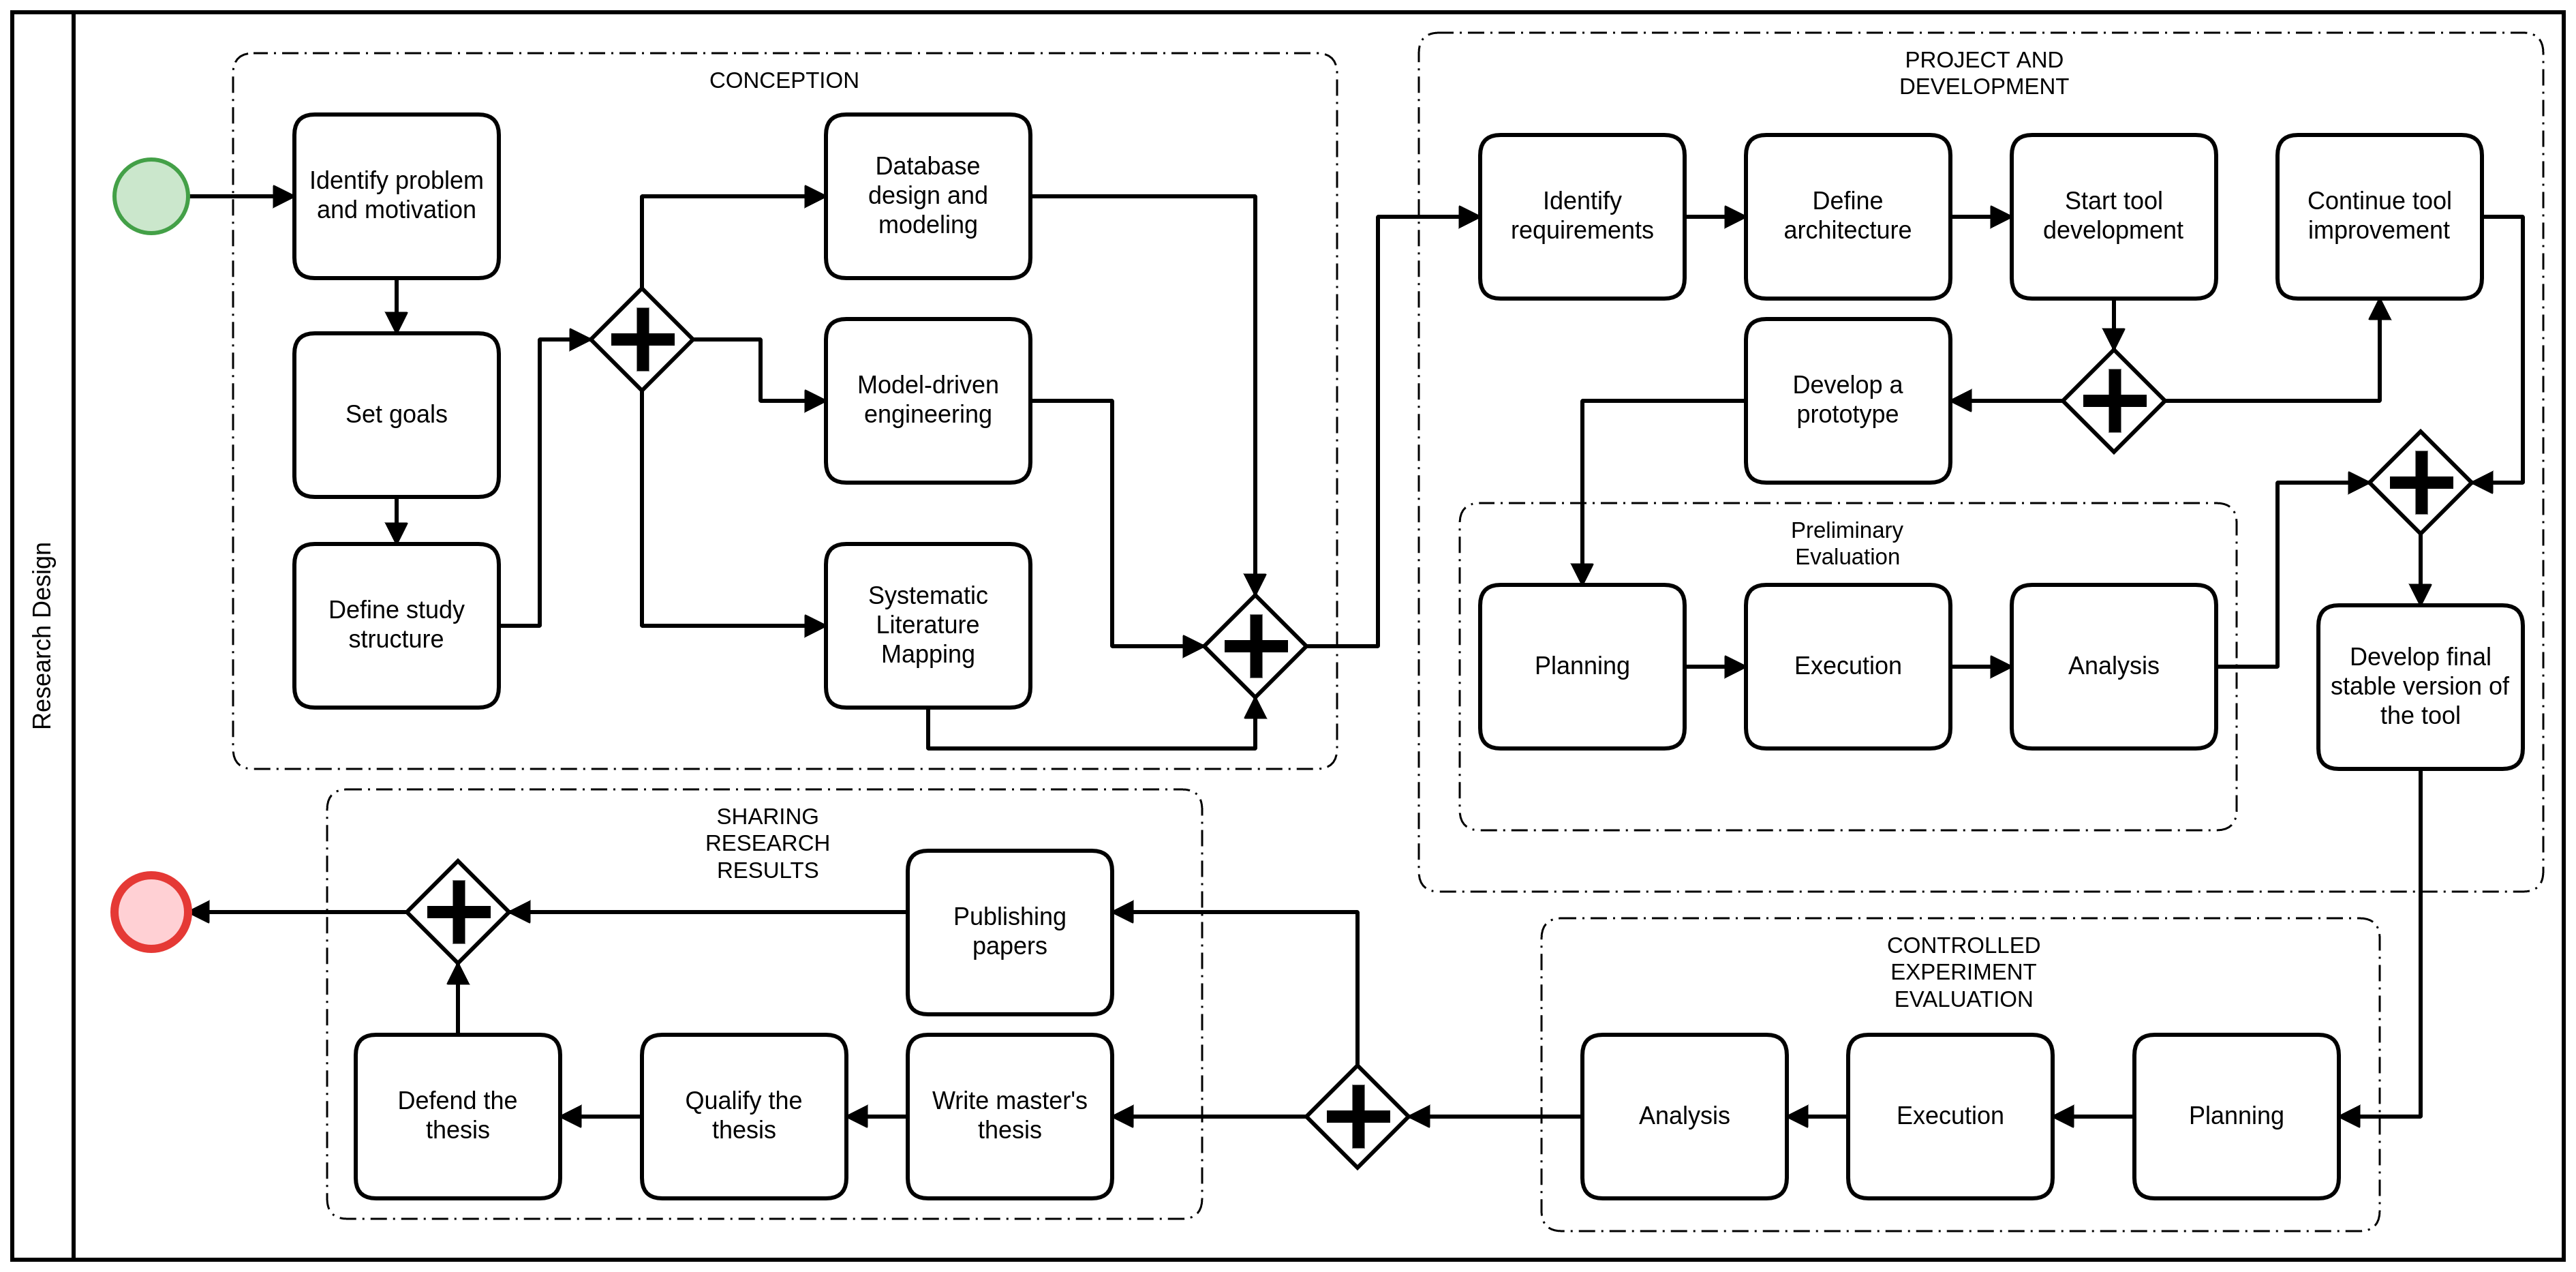
\includegraphics[width=1\textwidth]{img/ResearchDesign.png}
    \fonte{Author.}
    \label{fig:ResearchDesign}
\end{figure}

% O primeiro grupo corresponde a fase de concepção.
% Esta fase compreende na identificação do problema e motivação, no estabelecimento dos objetivos e a definição da estrutura do estudo.
% Para a criação de uma base teórica foram realizadas três atividades em paralelo, sendo o estudo sobre modelagem de projeto de bancos de dados, da engenharia dirigida por modelos e a execução de um mapeamento sistemático de literatura buscando mecanismos de transformação de modelos de bancos de dados relacionais.
The first group corresponds to the design phase.
This phase covers the identification of the problem and motivation, the establishment of objectives and the definition of the study structure.
To create a theoretical framework, three activities were carried out in parallel, namely the study of \ac{db} design modeling, model-driven engineering and the execution of a systematic literature mapping seeking mechanisms for transforming relational \ac{db} models.

% O segundo grupo corresponde a etapa de projeto e desenvolvimento da ferramenta.
% Foram identificados os requisitos, definida a arquitetura para então dar-se início no desenvolvimento da ferramenta. 
% De forma paralela, um protótipo passou por uma avaliação preliminar, descrita no Capítulo \ref{chap:evaluation}.
% Após ter os resultados analisados, provenientes da avaliação preliminar, é então gerado uma versão estável da ferramenta.
The second group covers the design and development stage of the tool.
The requirements were identified, the architecture was defined and then the development of the tool started.
In parallel, a prototype underwent a preliminary evaluation, described in Chapter \ref{chap:experiments}.
After having analyzed the results from the preliminary evaluation, a stable version of the tool is then generated.

% No terceiro grupo estão as atividades correspondentes a um experimento controlado ao qual esta versão estável será submetida, com o objetivo de avaliar todas as funções desenvolvidas. 
% Isso corresponde também a avaliação dos artefatos produzidos pelos geradores implementados: 
% È importante ressaltar que nenhum destes artefatos foram considerados na avaliação preliminar.
% In the third group are the activities corresponding to a controlled experiment to which this stable version will be submitted, with the objective of assess all the developed functions.
% This also corresponds to the evaluation of the artifacts produced by the implemented generators that were not considered in the preliminary evaluation:
% In the third group are the activities corresponding to a controlled experiment, in which we will submit this stable version, intending to evaluate all its features developed.
% It is also noteworthy that this corresponds to the evaluation of artifacts produced by the implemented generators, which we not considered in the preliminary evaluation:

% No terceiro grupo estão as atividades correspondentes aos últimos dois (2) experimentos controlados ao qual esta versão estável foi submetida, com o objetivo de avaliar todas as funções desenvolvidas. 
% Isso corresponde também a avaliação dos artefatos produzidos pelos geradores implementados: 
% È importante ressaltar que nenhum destes artefatos foram inicialmente considerados na primeira e segunda avaliações, mas apenas último experimento.
In the third group are the activities corresponding to the last two (2) controlled experiments to which this stable version was submitted, in order to evaluate all the functions developed.
This also corresponds to the evaluation of the artifacts produced by the implemented generators. 
It is important to emphasize that none of these artifacts were initially considered in the first and second evaluations, but only in the last experiment:

% \begin{itemize}
%     \item diagramas do modelo conceitual;
%     \item modelos lógicos em texto, no formato html;
%     \item modelos DDL (SQL) para DBMS específicos;
% \end{itemize}

\begin{itemize}
     \item Conceptual model diagrams;
     \item Logical textual models in \ac{html} format;
     \item \ac{ddl} templates for specific \acp{dbms}.
\end{itemize}

% Finalmente, o quarto grupo corresponde a divulgação dos resultados da pesquisa desenvolvida.
% Entre as atividades estão a escrita da dissertação e publicação de artigos em eventos científicos.
Finally, the fourth group corresponds to the dissemination of the results of the developed research.
Among the activities, we highlight the writing of the master's thesis and the paper's publishing in scientific events.

%------------------------------------------------------------------------------
% \section{Schedule}\label{met:schedule}
% 2021/02 previsto disciplina de BD em CC e ES
% O orientador é o professor da disciplina
% talvez chamar avaliação experimental
%------------------------------------------------------------------------------

% A Tabela \ref{tab:tableSchedule} apresenta o cronograma elaborado para as principais atividades previstas para a realização da dissertação de mestrado.
% As atividades são detalhadas quanto a sua duração conforme os meses que necessitam para serem completadas.
% Table \ref{tab:schedule} presents the schedule elaborated for the main activities foreseen for the accomplishment of the master's thesis.
% Activities are detailed in terms of duration according to the months they need to be completed.
% Table \ref{tab:schedule} presents the schedule elaborated for the main activities foreseen to accomplish the master's thesis.
% We detailed the activities in terms of duration according to the months they need to be completed.

% \section{Chapter Summary}\label{met:lessons}
% Descrever aprendizados
% se for descrever o capitulo, Chapter Summary

% Neste capítulo, apresentamos nossa metodologia de pesquisa.
% A classificação da pesquisa é importante para a realização adequada do planejamento das atividades necessárias para atingir o objetivo proposto neste estudo.
% Sendo assim, a partir de uma visão de alto nível de toda a nossa pesquisa é possível que um cronograma temporal seja detalhado, explicitando cada tarefa que deve ocorrer.
% In this chapter, we present our research methodology.
% The research classification is important for the proper planning of activities necessary to achieve the objective proposed in this study.
% Thus, from a high-level view of all our research, it is possible that a time schedule is detailed, explaining each task that must take place.
% In this chapter, we present our research methodology.
% The research classification is relevant to properly plan activities necessary to achieve the objective proposed in this study.
% Thus, from a high-level view of our entire research, we detail a schedule, explaining each task that must take place.

% \begin{landscape}
% \begin{table}[!htb]
% 	\centering
% 	\caption[Schedule.]{Schedule.}
% 	\label{tab:schedule}
% 	\resizebox{1.5\textwidth}{!}{\begin{tabular}{lc|cccccc|cccccc|cccccc|cc}
% 		\bottomrule
% 		\rowcolor[HTML]{C0C0C0}
% 		 & \multicolumn{1}{c|}{\textbf{2020/1}} & \multicolumn{6}{c|}{\textbf{2020/2}} & \multicolumn{6}{c|}{\textbf{2021/1}} & \multicolumn{6}{c|}{\textbf{2021/2}} & \multicolumn{2}{c}{\textbf{2022/1}}\\
% 		%\rowcolor[HTML]{C0C0C0}
% 		\textbf{Tasks} & \textbf{Jun} & \textbf{Jul} & \textbf{Aug} & \textbf{Sep} & \textbf{Oct} & \textbf{Nov} & \textbf{Dec} & \textbf{Jan} & \textbf{Feb} & \textbf{Mar} &  \textbf{Apr} & \textbf{May} & \textbf{Jun} & \textbf{Jul} & \textbf{Aug} & \textbf{Sep} & \textbf{Oct} & \textbf{Nov} & \textbf{Dec} & \textbf{Jan} & \textbf{Feb} \\ \hline
		
% 		\rowcolor[HTML]{C0C0C0}
% 		Tool Development & \checkmark & \checkmark & \checkmark & \checkmark & \checkmark & \checkmark & \checkmark & \checkmark & \checkmark & \checkmark & \checkmark & \checkmark & \checkmark & \checkmark & \checkmark & \checkmark & \checkmark & \checkmark & - & - & - \\
		
% 		Systematic Literature Mapping & - & - & - & \checkmark & \checkmark & \checkmark & \checkmark & - & - & - & - & - & - & - & - & - & - & - & - & - & - \\
		
% 		\rowcolor[HTML]{C0C0C0}
% 		Controlled Experiment 1 Planning & - & - & - & - & - & - & - & \checkmark & \checkmark & - & - & - & - & - & - & - & - & - & - & - & - \\
		
% 		Controlled Experiment 1 Execution & - & - & - & - & - & - & - & - & \checkmark & - & - & - & - & - & - & - & - & - & - & - & - \\
		
% 		\rowcolor[HTML]{C0C0C0}
% 		Controlled Experiment 1 Analysis & - & - & - & - & - & - & - & - & \checkmark & \checkmark & - & - & - & - & - & - & - & - & - & - & - \\
		
% 		Controlled Experiment 2 Planning & - & - & - & - & - & - & - & - & - & - & - & - & - & - & - & - & \checkmark & \checkmark & - & - & - \\
		
% 		\rowcolor[HTML]{C0C0C0}
% 		Controlled Experiment 2 Execution & - & - & - & - & - & - & - & - & - & - & - & - & - & - & - & - & - & \checkmark & \checkmark & - & - \\

% 		Controlled Experiment 2 Analysis & - & - & - & - & - & - & - & - & - & - & - & - & - & - & - & - & - & - & \checkmark & \checkmark & - \\
		
% 		\rowcolor[HTML]{C0C0C0}
% 		Writing and Publishing Articles & - & - & \checkmark & \checkmark & \checkmark & \checkmark & \checkmark & \checkmark & \checkmark & \checkmark & \checkmark & \checkmark & \checkmark & \checkmark & \checkmark & \checkmark & - & - & - & - & - \\
		
% 		Write Master's Thesis & - & - & - & - & - & - & - & - & - & - & - & - & - & - & - & - & - & \checkmark & \checkmark & \checkmark & \checkmark \\
		
% 		\toprule
% 	\end{tabular}}
% \end{table}
% \fonte{Author}
% \end{landscape}
%====================================================================
\chapter{Background}
\label{chap:background}
%====================================================================

% Este capítulo apresenta, de forma abrangente, os conceitos gerais utilizados para compreender e realizar este trabalho.
% A Seção \ref{sec_back:erModel} introduz o modelo entidade-relacionamento, bem como conceitos de modelos lógicos e físicos nas Seções \ref{sec_back:logicalModel} e \ref{sec_back:physicalModel}.
% A Seção \ref{sec_back:mde} apresenta a Model-Driven Engineering e assim suas noções associadas.
% Os conceitos referentes a Domain-Specific Languages são apresentadas na Seção \ref{sec_back:dsl}, seguido de Language Workbenches na Seção \ref{sec_back:LangWorkbench}.
% O Framework Xtext tem uma visão geral exibida na Seção \ref{sec_back:xtext} e, finalmente, as lições do capítulo são discutidas na Seção \ref{sec_back:lessons}.
This chapter presents the general concepts used to understand and implement this work in a comprehensive way.
Section \ref{sec_back:erModel} introduces the entity-relationship model as well as the concepts of logical and physical models in Sections \ref{sec_back:logicalModel} and \ref{sec_back:physicalModel}.
Section \ref{sec_back:mde} introduces Model-Driven Engineering and thus its associated notions.
The concepts referring to Domain-Specific Languages are presented in Section \ref{sec_back:dsl}, followed by Language Workbenches in Section \ref{sec_back:LangWorkbench}.
The Xtext Framework has an overview displayed in Section \ref{sec_back:xtext}, and finally, we discuss the lessons learned in Section \ref{sec_back:lessons}.

%------------------------------------------------------------------------------
\section{Entity-Relationship Model}
\label{sec_back:erModel}
%------------------------------------------------------------------------------

% O modelo conceitual de dados é a descrição de um banco de dado de forma independente da implementação utilizada em um SGBD. 
% Este modelo lista quais dados podem ocorrer no banco de dados, mas não registra como estes dados estão armazenados no nível de SGBD. 
% A técnica mais difundida de modelagem conceitual de dados é a \ac{er} de \cite{Chen:1976}. 
% Esta abordagem foi tão bem aceita que passou a ser considerada uma referência definitiva para a modelagem de bancos de dados relacionais. 
% É composta basicamente por um método de diagramação e de conceitos que devem ser respeitados. 
The conceptual data model is the description of a \ac{db} independently of the implementation used in a \ac{dbms}.
This model lists what data can occur in the \ac{db} but does not record how we stored this data at the \ac{dbms} level.
The most widespread technique of conceptual data modeling is the \ac{er} approach of \cite{Chen:1976}.
This approach was so well accepted that it is now considered a definitive reference for modeling relational \acp{db}.
It is primarily composed of a diagramming method and concepts that must be respected.

% Na abordagem \ac{er} o conceito principal é o de \textbf{entidade}, o qual é uma representação de um conjunto de objetos do domínio modelado \cite{Heuser:2009}. 
% As entidades são simbolizadas por retângulos. 
% Contudo, nesta abordagem ainda existem também outros conceitos que são essenciais e devem ser analisados.
% Para melhor compreensão da modelagem conceitual que utiliza esta abordagem, a seguir são apresentados na Figura \ref{fig:ERConstructors} algumas representações gráficas dos construtores previstos no modelo \ac{er}.
% In the \ac{er} approach, the principal concept is the \textbf{entity}, which is a representation of a set of objects from the modeled domain \cite{Heuser:2009}.
% Entities are symbolized by rectangles.
In the \ac{er} approach, the principal concept is the \textbf{entity}, representing a set of objects from the modeled domain \cite{Heuser:2009}. 
Rectangles symbolize the entities in the diagram. 
However, in this approach there are also other concepts that are essential and should be analyzed. 
For a better understanding of the conceptual modeling that uses this approach, Figure \ref{fig:ERConstructors} presents some graphical representations of the constructors foreseen in the \ac{er} model.

\begin{figure} [!htb]
    \centering
    \caption{ER Model Constructors.}
    \label{fig:ERConstructors}
    

\tikzset{every picture/.style={line width=0.75pt}} %set default line width to 0.75pt        

\begin{tikzpicture}[x=0.65pt,y=0.65pt,yscale=-1,xscale=1]
%uncomment if require: \path (0,597); %set diagram left start at 0, and has height of 597

%Shape: Rectangle [id:dp9409938961254447] 
\draw  [line width=1.5]  (29,15) -- (99,15) -- (99,55) -- (29,55) -- cycle ;

%Shape: Rectangle [id:dp25825363492065057] 
\draw  [line width=1.5]  (29,109.2) -- (99,109.2) -- (99,149.2) -- (29,149.2) -- cycle ;
%Shape: Rectangle [id:dp9273607878616594] 
\draw  [line width=1.5]  (33.2,112.8) -- (94.8,112.8) -- (94.8,145.6) -- (33.2,145.6) -- cycle ;

%Shape: Diamond [id:dp07590485693463012] 
\draw  [line width=1.5]  (68.65,282) -- (99.3,298.5) -- (68.65,315) -- (38,298.5) -- cycle ;

%Shape: Diamond [id:dp8393196312653484] 
\draw  [line width=1.5]  (70,383) -- (102.71,400.61) -- (70,418.22) -- (37.29,400.61) -- cycle ;
%Shape: Diamond [id:dp11016744869268091] 
\draw  [line width=1.5]  (70,387.11) -- (95.08,400.61) -- (70,414.11) -- (44.92,400.61) -- cycle ;

%Shape: Ellipse [id:dp8577075014649969] 
\draw   (212.43,122.3) .. controls (212.43,115.07) and (222.69,109.2) .. (235.35,109.2) .. controls (248.01,109.2) and (258.28,115.07) .. (258.28,122.3) .. controls (258.28,129.53) and (248.01,135.4) .. (235.35,135.4) .. controls (222.69,135.4) and (212.43,129.53) .. (212.43,122.3) -- cycle ;
%Straight Lines [id:da240419684606217] 
\draw    (193.72,122.5) -- (212.43,122.3) ;


%Shape: Ellipse [id:dp11655523259938039] 
\draw  [fill={rgb, 255:red, 0; green, 0; blue, 0 }  ,fill opacity=1 ] (212.43,28.1) .. controls (212.43,20.87) and (222.69,15) .. (235.35,15) .. controls (248.01,15) and (258.28,20.87) .. (258.28,28.1) .. controls (258.28,35.33) and (248.01,41.2) .. (235.35,41.2) .. controls (222.69,41.2) and (212.43,35.33) .. (212.43,28.1) -- cycle ;
%Straight Lines [id:da7122954732701139] 
\draw    (193.72,28.3) -- (212.43,28.1) ;


%Shape: Ellipse [id:dp23076223718363464] 
\draw  [line width=1.5]  (212.43,213.5) .. controls (212.43,206.27) and (222.69,200.4) .. (235.35,200.4) .. controls (248.01,200.4) and (258.28,206.27) .. (258.28,213.5) .. controls (258.28,220.74) and (248.01,226.6) .. (235.35,226.6) .. controls (222.69,226.6) and (212.43,220.74) .. (212.43,213.5) -- cycle ;
%Straight Lines [id:da42071644925844054] 
\draw    (193.72,213.7) -- (212.43,213.5) ;
%Shape: Ellipse [id:dp409593727665448] 
\draw  [line width=1.5]  (216.22,213.5) .. controls (216.22,207.99) and (224.78,203.51) .. (235.35,203.51) .. controls (245.92,203.51) and (254.48,207.99) .. (254.48,213.5) .. controls (254.48,219.02) and (245.92,223.49) .. (235.35,223.49) .. controls (224.78,223.49) and (216.22,219.02) .. (216.22,213.5) -- cycle ;


%Shape: Ellipse [id:dp12298573968430726] 
\draw   (203.9,406.37) .. controls (203.9,402.67) and (209.15,399.67) .. (215.63,399.67) .. controls (222.11,399.67) and (227.36,402.67) .. (227.36,406.37) .. controls (227.36,410.07) and (222.11,413.07) .. (215.63,413.07) .. controls (209.15,413.07) and (203.9,410.07) .. (203.9,406.37) -- cycle ;
%Straight Lines [id:da026255036427652145] 
\draw    (187.96,406.53) -- (203.9,406.37) ;
%Shape: Ellipse [id:dp035873659384954015] 
\draw   (228.96,388.9) .. controls (228.96,385.2) and (234.21,382.2) .. (240.69,382.2) .. controls (247.17,382.2) and (252.42,385.2) .. (252.42,388.9) .. controls (252.42,392.61) and (247.17,395.61) .. (240.69,395.61) .. controls (234.21,395.61) and (228.96,392.61) .. (228.96,388.9) -- cycle ;
%Straight Lines [id:da0884897826197295] 
\draw    (220.87,400.43) -- (230.56,392.66) ;
%Shape: Ellipse [id:dp33703819371371857] 
\draw   (240.57,406.54) .. controls (240.57,402.84) and (245.83,399.84) .. (252.31,399.84) .. controls (258.78,399.84) and (264.04,402.84) .. (264.04,406.54) .. controls (264.04,410.24) and (258.78,413.24) .. (252.31,413.24) .. controls (245.83,413.24) and (240.57,410.24) .. (240.57,406.54) -- cycle ;
%Straight Lines [id:da041465674734754376] 
\draw    (227.45,406.65) -- (240.57,406.54) ;
%Shape: Ellipse [id:dp8994114077261279] 
\draw   (228.96,422.06) .. controls (228.96,418.36) and (234.21,415.36) .. (240.69,415.36) .. controls (247.17,415.36) and (252.42,418.36) .. (252.42,422.06) .. controls (252.42,425.77) and (247.17,428.77) .. (240.69,428.77) .. controls (234.21,428.77) and (228.96,425.77) .. (228.96,422.06) -- cycle ;
%Straight Lines [id:da5145813744043246] 
\draw    (220.73,412.57) -- (230.48,418.83) ;


%Shape: Triangle [id:dp717941434970198] 
\draw  [line width=1.5]  (374.97,15) -- (401.3,51.2) -- (348.65,51.2) -- cycle ;

%Shape: Triangle [id:dp8547281306342895] 
\draw  [line width=1.5]  (486.97,51.2) -- (460.65,15) -- (513.3,15) -- cycle ;

%Shape: Ellipse [id:dp057823722753663986] 
\draw  [dash pattern={on 5.63pt off 4.5pt}][line width=1.5]  (212.43,305.1) .. controls (212.43,297.87) and (222.69,292) .. (235.35,292) .. controls (248.01,292) and (258.28,297.87) .. (258.28,305.1) .. controls (258.28,312.33) and (248.01,318.2) .. (235.35,318.2) .. controls (222.69,318.2) and (212.43,312.33) .. (212.43,305.1) -- cycle ;
%Straight Lines [id:da4937273930595423] 
\draw    (193.72,305.3) -- (212.43,305.1) ;


%Shape: Diamond [id:dp8682093873982866] 
\draw  [line width=1.5]  (426.11,109.2) -- (457.39,127.6) -- (426.11,146) -- (394.83,127.6) -- cycle ;
%Shape: Rectangle [id:dp16263593596228687] 
\draw  [line width=1.5]  (319.8,113.94) -- (365.03,113.94) -- (365.03,140.15) -- (319.8,140.15) -- cycle ;
%Shape: Rectangle [id:dp9045715408610813] 
\draw  [line width=1.5]  (486.57,115.67) -- (531.8,115.67) -- (531.8,141.89) -- (486.57,141.89) -- cycle ;
%Straight Lines [id:da894737740624673] 
\draw [line width=1.5]    (366.09,127.03) -- (394.83,127.6) ;
%Straight Lines [id:da45477038200691244] 
\draw [line width=1.5]    (457.39,127.6) -- (486.13,128.17) ;


%Shape: Diamond [id:dp8788662265812572] 
\draw  [line width=1.5]  (426.12,238.62) -- (457.82,257.27) -- (426.12,275.92) -- (394.41,257.27) -- cycle ;
%Shape: Rectangle [id:dp7607057696775741] 
\draw  [line width=1.5]  (318.35,243.42) -- (364.2,243.42) -- (364.2,270) -- (318.35,270) -- cycle ;
%Shape: Rectangle [id:dp20655084709944105] 
\draw  [line width=1.5]  (487.4,245.18) -- (533.25,245.18) -- (533.25,271.76) -- (487.4,271.76) -- cycle ;
%Straight Lines [id:da33926375234409023] 
\draw [line width=1.5]    (365.28,256.69) -- (394.41,257.27) ;
%Straight Lines [id:da8300796405989177] 
\draw [line width=1.5]    (457.82,257.27) -- (486.95,257.85) ;
%Shape: Rectangle [id:dp11640389244166749] 
\draw  [line width=1.5]  (402.47,300.05) -- (448.32,300.05) -- (448.32,326.63) -- (402.47,326.63) -- cycle ;
%Straight Lines [id:da04160890165480735] 
\draw [line width=1.5]    (425.88,299.64) -- (426.12,275.92) ;


%Shape: Diamond [id:dp09298931741553762] 
\draw  [line width=1.5]  (116.43,486.83) -- (136.89,498.86) -- (116.43,510.89) -- (95.98,498.86) -- cycle ;
%Shape: Rectangle [id:dp7562868332770196] 
\draw  [line width=1.5]  (24.66,482.2) -- (84.33,482.2) -- (84.33,516.79) -- (24.66,516.79) -- cycle ;
%Straight Lines [id:da5257649797909345] 
\draw [line width=1.5]    (84.98,510.57) -- (116.43,510.89) ;

%Straight Lines [id:da741474729938117] 
\draw [line width=1.5]    (83.76,486.58) -- (116.43,486.83) ;

%Shape: Diamond [id:dp27975998103917443] 
\draw  [line width=1.5]  (424.23,422.01) -- (446.41,435.06) -- (424.23,448.11) -- (402.04,435.06) -- cycle ;
%Shape: Rectangle [id:dp27388026856661996] 
\draw  [line width=1.5]  (348.82,425.37) -- (380.9,425.37) -- (380.9,443.97) -- (348.82,443.97) -- cycle ;
%Shape: Rectangle [id:dp8682931511633045] 
\draw  [line width=1.5]  (467.12,426.6) -- (499.19,426.6) -- (499.19,445.2) -- (467.12,445.2) -- cycle ;
%Straight Lines [id:da8247964733470876] 
\draw [line width=1.5]    (381.66,434.65) -- (402.04,435.06) ;
%Straight Lines [id:da507174915044009] 
\draw [line width=1.5]    (446.41,435.06) -- (466.8,435.46) ;
%Shape: Diamond [id:dp489563487309699] 
\draw  [line width=1.5]  (423.82,465.94) -- (446,478.99) -- (423.82,492.04) -- (401.63,478.99) -- cycle ;
%Straight Lines [id:da8803188939906841] 
\draw [line width=1.5]    (423.85,453.98) -- (423.82,465.94) ;
%Shape: Rectangle [id:dp2462964817052231] 
\draw  [line width=1.5]  (407.53,500.09) -- (439.61,500.09) -- (439.61,518.68) -- (407.53,518.68) -- cycle ;
%Straight Lines [id:da17335151983105646] 
\draw [line width=1.5]    (423.82,492.04) -- (423.83,500.08) ;
%Shape: Rectangle [id:dp019446741600327666] 
\draw  [line width=1.5]  (344.3,417.82) -- (503.3,417.82) -- (503.3,453.62) -- (344.3,453.62) -- cycle ;


%Shape: Rectangle [id:dp7508437049659447] 
\draw  [line width=1.5]  (27.54,200.66) -- (100.46,200.66) -- (100.46,242.94) -- (27.54,242.94) -- cycle ;
%Shape: Diamond [id:dp4714864707556645] 
\draw  [line width=1.5]  (64,200.4) -- (100.38,221.8) -- (64,243.2) -- (27.62,221.8) -- cycle ;



% Text Node
\draw (64,70) node  [font=\footnotesize] [align=left] {Entity};
% Text Node
\draw (64,88) node  [font=\footnotesize] [align=left] {(Strong)};
% Text Node
\draw (64,164.2) node  [font=\footnotesize] [align=left] {Weak Entity};
% Text Node
\draw (226,55.1) node   [align=left] {{\footnotesize Referential Attribute}};
% Text Node
\draw (226,447) node  [font=\footnotesize] [align=left] {Composite};
% Text Node
\draw (226,467) node  [font=\footnotesize] [align=left] {Attribute};
% Text Node
\draw (226,149.3) node   [align=left] {{\footnotesize Descriptive Attribute}};
% Text Node
\draw (226,169.3) node   [align=left] {{\footnotesize (Simple)}};
% Text Node
\draw (68.65,334.8) node  [font=\footnotesize] [align=left] {Relationship};
% Text Node
\draw (68.65,354.8) node  [font=\footnotesize] [align=left] {(Strong)};
% Text Node
\draw (70,436.8) node  [font=\footnotesize] [align=left] {Dependent Relationship};
% Text Node
\draw (70,456.8) node  [font=\footnotesize] [align=left] {(Weak)};
% Text Node
\draw (226,240.5) node   [align=left] {{\footnotesize Multivalued}};
% Text Node
\draw (226,259.5) node   [align=left] {{\footnotesize Attribute}};
% Text Node
\draw (489,69) node  [font=\footnotesize] [align=left] {Specialization};
% Text Node
\draw (226,336.1) node   [align=left] {{\footnotesize Derived Attribute}};
% Text Node
\draw (378,70) node  [font=\footnotesize] [align=left] {Generalization};
% Text Node
\draw (425.8,352.42) node  [font=\footnotesize] [align=left] {N-ary Relationship};
% Text Node
\draw (425.8,173.22) node  [font=\footnotesize] [align=left] {Binary Relationship};
% Text Node
\draw (423.8,541.2) node  [font=\footnotesize] [align=left] {Aggregation};
% Text Node
\draw (80.78,538.2) node  [font=\footnotesize] [align=left] {Recursive Relationship};
% Text Node
\draw (80.78,556.2) node  [font=\footnotesize] [align=left] {(Self Relationship)};
% Text Node
\draw (64,262.2) node   [align=left] {{\footnotesize Associative Entity}};


\end{tikzpicture}

    \fonte{Author.}
\end{figure}

% Uma \textbf{Entidade Forte} e uma entidade que para existir não depende da existência de outra(s) entidades(s). 
% De forma inversa, uma \textbf{Entidade Fraca} é uma entidade que possui sua existência ou identificação dependente de outra(s) entidade(s). 
% A representação de \textbf{Entidade Associativa} serve para dar mais sentido semântico ao modelo, e pode ser usada para simbolizar relações muitos para muitos, contendo referências a colunas de tabelas do mesmo ou de outros \acp{db}.
A \textbf{strong entity} is an entity that does not depend on the existence of other entity(ies) to exist.
Conversely, a \textbf{weak entity} is an entity that has its existence or identification dependent on other entity(ies).
An \textbf{associative entity} serves to give more semantic meaning to the model and to symbolize many-to-many relationships, containing references to columns of tables of the same or other \acp{db}.

% Os \textbf{atributos} podem ser \textbf{referenciais}, ou seja, que identificam a entidade, e \textbf{descritivos} que a descrevem. 
% A maioria dos atributos tendem a ser descritivos e também são chamados de simples ou monovalorados. 
% Contudo, existem outros tipos destes atributos como os \textbf{multivalorados}, que podem assumir diversos valores, os \textbf{derivados}, que são inferidos a partir de outros atributos, e os \textbf{compostos}, que podem ser divididos em várias partes com significados independentes.
The \textbf{attributes} can be \textbf{referential}, that is, they identify the entity, and \textbf{descriptive} that describe it.
Most attributes tend to be descriptive and are also called simple or single-valued.
However, there are other types of these attributes such as \textbf{multi-valued}, which can take different values, \textbf{derived}, which are inferred from other attributes, and \textbf{composite} attributes, which can be divided into several parts with independent meanings.

% No que diz respeito aos \textbf{relacionamentos} possíveis entre entidades pode-se citar os \textbf{binários}, aqueles que envolvem duas (2) entidades, e os \textbf{n-ários} que correspondem a ligação de três (3) ou mais entidades. 
% É comum que as relações compostas especificamente por três entidades sejam chamadas de relações \textbf{ternárias}. 
% Além destes tipos ainda é possível haver relações recursivas de uma entidade com ela mesma, também chamado de \textbf{auto-relacionamento}.
Regarding the possible \textbf{relationships} between entities, we can mention the \textbf{binary} that involve two (2) entities and the \textbf{n-ary} that correspond to the link of three (3) or more entities.
It is common for relations composed of three entities to be called \textbf{ternary} relations.
Besides these types, it is still possible to have recursive relationships of an entity with itself, also called \textbf{self-relationship}.

% A abordagem \ac{er} ainda suporta conceitos de \textbf{generalização/especialização}, que definem um grupo hierárquico de entidades que compartilham atributos em comum, e \textbf{agregação} onde a condição de existência é que o relacionamento principal necessita ser necessariamente de muitos para muitos.
The \ac{er} approach still supports concepts of \textbf{generalization/specialization}, which define a hierarchical group of entities that share common attributes, and \textbf{aggregation} where the existence condition is that the principal relationship needs to be necessarily from many-to-many.

% Os \textbf{relacionamentos} representam a associação entre os objetos e são sinalizados por losangos. 
% A \textbf{cardinalidade} de relacionamentos registra o número de ocorrências com que as entidades podem se associar. 
% Existem duas cardinalidades que devem ser atribuídas: a mínima e a máxima. 
% Os \textbf{atributos} são características representadas por pequenos círculos conectados as entidades. 
The \textbf{relationships} represent the association among objects, and diamonds denote them.
The \textbf{cardinality} of relationships records the number of occurrences that entities can associate with each other.
Two cardinalities must be assigned: the minimum and the maximum. \textbf{Attributes} are features represented by small circles connected to entities.

%------------------------------------------------------------------------------
\section{Logical Model}
\label{sec_back:logicalModel}
%------------------------------------------------------------------------------

% Um modelo lógico de dados é definido como um modelo que possui a representação dos objetos, relacionamentos e características de acordo com regras de implementação. 
% Isso significa que esse modelo tem um nível de abstração do ponto de vista do usuário de um \ac{dbms}. 
% Ainda assim, o modelo lógico é independente do tipo de \ac{dbms} em que é implementado. 
A logical data model defines a model that represents objects, relationships, and characteristics according to implementation rules.
This means that this model has a level of abstraction from the user's point of view of a \ac{dbms}.
Still, the logical model is independent of the type of \ac{dbms} in which that implements it.

% Esse tipo de modelo deve necessariamente respeitar conceitos tais como chaves de acesso, controle de chaves duplicadas, normalização, integridade referencial, controle de redundância de dados, entre outros. 
% Este modelo é intrinsecamente relacionado a fase de projeto \cite{Cougo:2013}. 
% É importante salientar que essa é uma forma direcionada a um aspecto gráfico, porém existem meios alternativos de se representar estruturalmente o mesmo modelo de forma textual \cite{Martelli:2018}. 
This type of model must necessarily respect concepts such as access keys, duplicate keys control, normalization, referential integrity, data redundancy control, among others.
This model is intrinsically related to the design phase \cite{Cougo:2013}.
% It is important to point out that this is a form directed to a graphic aspect, but there are alternative ways to structurally represent the same model in a textual form \cite{Martelli:2018}.
It is worth pointing out that this is a directed way to graphical aspect, but there are alternative ways to represent the same structurally model in a textual form \cite{Martelli:2018}.

%------------------------------------------------------------------------------
\section{Physical Model}
\label{sec_back:physicalModel}
%------------------------------------------------------------------------------

% Um modelo físico de dados caracteriza-se como um modelo em que a representação dos objetos de \ac{db} já estão em um nível físico de implementação das ocorrências, ou instâncias, das entidades de relacionamentos. 
% Cada \ac{dbms} pode definir diferentes modos de implementação física das características e recursos indispensáveis para o armazenamento e manipulação das estruturas de dados \cite{Cougo:2013}.
A physical data model characterizes as a model in which the \ac{db} objects representation are already at a physical level of implementation of the occurrences (or instances) of the entities of relationships.
Each \ac{dbms} can define different modes of physical implementation, involving characteristics and essential resources for the storage and manipulation of data structures. \cite{Cougo:2013}.

% Em geral os modelos físicos apresentam dois aspectos bem representados. 
% Primeiramente, existem as ocorrências ou instâncias, seus relacionamentos e a disposição básica dos elementos. 
% O outro aspecto diz respeito a alocação nos diversos níveis de agrupamentos possíveis, como as tabelas, linhas (registros), colunas (campos) e blocos \cite{West:2011}.
% Em suma, é a materialização dos objetos de \ac{db} em um esquema interno de um dado \ac{dbms} a partir da execução de uma sequência lógica de instruções em \ac{sql}.
In general, physical models have two well-represented aspects.
First, there are the occurrences or instances, their relationships, and the basic arrangement of elements.
The other aspect concerns the allocation in the different levels of possible groupings, such as tables, rows (records), columns (fields), and blocks \cite{West:2011}.
In short, it is the materialization of \ac{db} objects in an internal schema of a given \ac{dbms} from the execution of a logical sequence of instructions in \ac{sql}.

%------------------------------------------------------------------------------
\section{Model-Driven Engineering}
\label{sec_back:mde}
%------------------------------------------------------------------------------

% Conceitualmente um modelo é uma representação, protótipo ou exemplo que se tem por objetivo reproduzir ou imitar alguma forma. 
% A construção de modelos são pontos centrais e importantes em diferentes áreas científicas. 
% Na matemática, física, engenharia e química, por exemplo, o emprego de modelos é tido como vital para a investigação teórica e prática em diferentes campos de estudo \cite{Bailer:2009}.
A model is, conceptually, a representation, prototype or example that has the objective of reproducing or imitating something in some way.
Model building is central and relevant in different scientific areas.
In mathematics, physics, engineering, and chemistry areas, for example, the use of models is considered vital for theoretical and practical research in different fields of study \cite{Bailer:2009}.

% A \ac{mde}, ou \ac{mdse}, é um campo da Engenharia de Software que tem sua origem a partir da criação das primeiras ferramentas CASE surgidas nos anos 1980.
% Enquanto subárea da Engenharia de Software, a \ac{mde} é uma abordagem que preconiza essencialmente que um processo de desenvolvimento tenha modelos como principais saídas (ou também como entradas) de alguma atividade.  
% Esta abordagem tem como objetivo maximizar a produtividade, a compatibilidade entre sistemas (através da reutilização de modelos) e simplificar a complexidade envolvida no processo de projeto de software \cite{Brambilla:2017}. 
% Dessa forma, isto resulta em programas ou atividades de computador executados em hardware ou software que são gerados automaticamente a partir de modelos \cite{Sommerville:2011}. 
\ac{mde}, or \ac{mdse}, is a field of Software Engineering that has its origins since the creation of the first \ac{case} tools that emerged in the 1980s.
As a sub-area of Software Engineering, \ac{mde} is an approach that essentially calls for a development process to have models as the main inputs (or also outputs) of some activity.
This approach aims to maximize productivity, compatibility between systems (through model reuse) and simplify the complexity involved in the software design process  \cite{Brambilla:2017}.
In this way, this results in programs or computer activities executed in hardware or software that are automatically generated from models \cite{Sommerville:2015}.

% Esta área de estudo vem evoluindo consideravelmente desde os anos 1990. 
% Em resumo,  a MDE fez contribuições para potencializar a abstração, visando assim a automação, em quase todas as áreas de desenvolvimento e análise \cite{Bucchiarone:2020}. 
% Essas contribuições podem ser identificadas em diversos domínios onde modelos são indispensáveis para o sucesso e.g. sistemas de software, sistemas de transporte, indústria automotiva, processos de negócio, biotecnologia e genética. 
% Conceitualmente, a \ac{mde} fornece apoio a outros conceitos, como o \ac{mdd} e a \ac{mda}. Na Figura \ref{fig:MDE} a relação entre estes conceitos é ilustrada
This area of study has been evolving considerably since the 1990s.
In short, MDE has made contributions to leverage abstraction, thus aiming at automation, in almost all areas of development and analysis \cite{Bucchiarone:2020}.
These contributions identified in several domains where models are indispensable for success e.g. software systems, transport systems, automotive industry, business processes, biotechnology, and genetics.
Conceptually, \ac{mde} supports other concepts such as \ac{mdd} and \ac{mda}. 
Figure \ref{fig:MDE} illustrates the relationship among these concepts.
% In Figure \ref{fig:MDE} the relationship between these concepts is illustrated.

\begin{figure}[!htb]
    \centering
    \caption{Relationship among MDE, MDD and MDA.}
    

\tikzset{every picture/.style={line width=0.75pt}} %set default line width to 0.75pt        

\begin{tikzpicture}[x=0.75pt,y=0.75pt,yscale=-1,xscale=1]
%uncomment if require: \path (0,300); %set diagram left start at 0, and has height of 300

%Shape: Ellipse [id:dp03875628946363818] 
\draw  [fill={rgb, 255:red, 255; green, 255; blue, 255 }  ,fill opacity=1 ] (91,113.58) .. controls (91,67.97) and (171.7,31) .. (271.25,31) .. controls (370.8,31) and (451.5,67.97) .. (451.5,113.58) .. controls (451.5,159.18) and (370.8,196.15) .. (271.25,196.15) .. controls (171.7,196.15) and (91,159.18) .. (91,113.58) -- cycle ;
%Shape: Ellipse [id:dp565416950765411] 
\draw  [fill={rgb, 255:red, 255; green, 255; blue, 255 }  ,fill opacity=1 ] (136.74,134.53) .. controls (136.74,100.49) and (196.96,72.9) .. (271.25,72.9) .. controls (345.54,72.9) and (405.76,100.49) .. (405.76,134.53) .. controls (405.76,168.56) and (345.54,196.15) .. (271.25,196.15) .. controls (196.96,196.15) and (136.74,168.56) .. (136.74,134.53) -- cycle ;
%Shape: Ellipse [id:dp0635650382067301] 
\draw  [fill={rgb, 255:red, 255; green, 255; blue, 255 }  ,fill opacity=1 ] (179.42,155.65) .. controls (179.42,132.41) and (220.53,113.58) .. (271.25,113.58) .. controls (321.97,113.58) and (363.08,132.41) .. (363.08,155.65) .. controls (363.08,178.88) and (321.97,197.72) .. (271.25,197.72) .. controls (220.53,197.72) and (179.42,178.88) .. (179.42,155.65) -- cycle ;

% Text Node
\draw (271.25,52) node  [font=\Large] [align=left] {MDE};
% Text Node
\draw (271.25,93) node  [font=\Large] [align=left] {MDD};
% Text Node
\draw (271.25,134.65) node  [font=\Large] [align=left] {MDA};


\end{tikzpicture}

    \fonte{Adapted from \cite{Ameller:2009}}
    \label{fig:MDE}
\end{figure}

% O \ac{mdd} é um paradigma de desenvolvimento que usa modelos como principais artefatos em um processo de desenvolvimento. 
% No \ac{mdd} geralmente a implementação é gerada de forma automática ou semiautomática a partir dos modelos. 
% Apesar de serem vistas como a mesma coisa, os conceitos estabelecidos na literatura acerca da \ac{mde} e da \ac{mdd} tem origem direta na \ac{mda}, formalmente proposta inicialmente em 2001 pela \ac{omg}\footnote{MDA Guide 2.0: \url{ https://www.omg.org/cgi-bin/doc?ormsc/14-06-01.pdf}}. 
\ac{mdd} is a development paradigm that uses models as principal artifacts in a development process.
In \ac{mdd}, the implementation is usually generated automatically or semi-automatically from the models.
Despite being seen as the same thing, the concepts established in the literature about \ac{mde} and \ac{mdd} have direct origins in \ac{mda}, first formally proposed only in 2001 by \ac{omg}\footnote{MDA Guide 2.0: \url{ https://www.omg.org/cgi-bin/doc?ormsc/14-06-01.pdf}}.

% Segundo \cite{Sommerville:2015} as diferenças são sutis, uma vez que a \ac{mda} concentra-se nos estágios de projeto e implementação do processo de desenvolvimento de software, sendo muito similar ao \ac{mdd}, porém implementando diretrizes específicas da \ac{omg}. 
% Isso faz com que os processos de \ac{mdd} se utilizem de diversas abstrações para esconder, ou até mesmo remover, detalhes que possam eventualmente tornar um modelo mais complexo. 
According to \cite{Sommerville:2015}, the differences are subtle since \ac{mda} focuses on the design and implementation stages of the software development process, being very similar to \ac{mdd}, however implementing \ac{omg}-specific guidelines.
Hence, this causes the \ac{mdd} processes to use various abstractions to hide, or even remove, details that could eventually make a model more complex.

% Dito isto, conclui-se que a \ac{mda} é um subconjunto do \ac{mdd}. 
% Por outro lado, a \ac{mde} pode abordar muitos outros tópicos dos processos de Engenharia de Software, entre eles a engenharia de requisitos baseada em modelos, processos de software para desenvolvimento baseado em modelos, ou ainda, testes baseados em modelos.
% A \ac{mde}, como uma metodologia, auxilia a aplicação das vantagens da modelagem nas atividades de Engenharia de Software. 
% Para \cite{Brambilla:2017} essa abordagem leva em consideração quatro aspectos fundamentais, listados a seguir.

Once that is said, it follows that \ac{mda} is a subset of \ac{mdd}.
On the other hand, \ac{mde} can address many others topics in Software Engineering processes, including model-based requirements engineering, model-based software processes for development, or even model-based testing.
\ac{mde}, as a methodology, helps to apply the advantages of modeling in Software Engineering activities.
For \cite{Brambilla:2017}, this approach takes into consideration four fundamental aspects listed below.

% \begin{enumerate}
%   \item Conceitos: os componentes que constroem a metodologia, abrangendo desde artefatos de linguagem até atores, e assim por diante;
%   \item Notações: A maneira como os conceitos são representados, ou seja, as linguagens usadas na metodologia;
%   \item Processos e Regras: As atividades que levam à elaboração do produto final, as regras para sua administração e controle, e as afirmações sobre as propriedades desejadas (correção, consistência, etc) dos produtos ou do próprio processo;
%   \item Ferramentas: Aplicações que facilitam a execução de atividades ou seu controle, abrangendo o processo de produção e apoiando o desenvolvedor no uso das notações.
% \end{enumerate}

\begin{enumerate}
   \item \textbf{Concepts}: the components that build the methodology, ranging from language artifacts to actors, and so forth;
   \item \textbf{Notations}: The way concepts are represented, \textit{i.e.} the languages used in the methodology;
   \item \textbf{Processes and Rules}: The activities that lead to the elaboration of the final product, the rules for its administration and control, and the statements about the desired properties (correction, consistency, etc) of the products or of the process itself;
   \item \textbf{Tools}: Applications that facilitate the execution of activities or their control, covering the production process, and supporting the developer in the use of notations.
\end{enumerate}

% A motivação por trás da \ac{mde} é a ideia de se aumentar o nível de abstração do processo de desenvolvimento em geral, para então assim capturar sistemas ou processos como uma coleção de modelos reutilizáveis. 
% Logo, ela visa reduzir a dificuldade associada ao desenvolvimento de sistemas de software, em geral mais complexos, por meio do uso de técnicas de modelagem que suportam a separação de interesses e geração automatizada de artefatos de sistemas a partir de modelos \cite{Batory:2015, Kleppe:2003}.
The motivation behind \ac{mde} is increasing the abstraction level of the development process in general and then capturing processes or systems as a collection of reusable models.
Therefore, it aims to reduce the difficulty associated with the development of software systems, which are generally more complex, through the modeling techniques implementation that supports the separation of interests and the automated generation of system artifacts from models \cite{Batory:2015, Kleppe:2003}.
% Therefore, it aims to reduce the difficulty associated with developing software systems, which are generally more complex, through the use of modeling techniques that support the separation of interests and automated generation of system artifacts from models \cite{Batory:2015, Kleppe:2003}.

% De uma forma objetiva, a abordagem \ac{mda} define uma estrutura para se realizar a \ac{mde}, ou também ainda a \ac{mdd}. 
% Essa abordagem define três camadas que devem ser usadas como pilares para todo o processo \cite{Frantz:2012}, listados a seguir.
% A relação conceitual entre esses níveis, com o uso de mecanismos de transformação e regras de transformação, é exemplificado na Figura \ref{fig:MDA}.

Objectively, the \ac{mda} approach defines a structure to perform the \ac{mde}, or also the \ac{mdd}.
% This approach defines three layers that should be used as pillars for the whole process \cite{Frantz:2012} listed below.
This approach defines three layers used as pillars for the whole process \cite{Frantz:2012} listed below.
The conceptual relationship between these levels, using transformation mechanisms and transformation rules, is exemplified in Figure \ref{fig:MDA}.

% \begin{enumerate}
%     \item \acp{CIM}: descrevem objetos de negócio e as atividades independentemente de sistemas de suporte;
%     \item \acp{PIM}: descrevem como os processos de negócio são suportados por sistemas, vistos como caixas-pretas funcionais, ou seja, desconsiderando as restrições associadas às tecnologias candidatas;
%     \item \acp{PSM}: descrevem os componentes do sistema conforme implementados por tecnologias específicas.
% \end{enumerate}
\begin{enumerate}
     \item \textbf{\acp{cim}}: describe business objects and activities independently from support systems;
     \item \textbf{\acp{pim}}: describe how business processes are supported by systems, seen as functional black boxes, \textit{i.e.} disregarding the restrictions associated with candidate technologies;
     \item \textbf{\acp{psm}}: describe system components as implemented by specific technologies.
\end{enumerate}

\begin{figure}[!htb]
    \centering
    \caption{MDA abstraction levels.}
    

\tikzset{every picture/.style={line width=0.75pt}} %set default line width to 0.75pt        

\begin{tikzpicture}[x=0.75pt,y=0.75pt,yscale=-1,xscale=1]
%uncomment if require: \path (0,442); %set diagram left start at 0, and has height of 442

%Shape: Rectangle [id:dp7655816759589134] 
\draw  [fill={rgb, 255:red, 255; green, 255; blue, 255 }  ,fill opacity=1 ][line width=1.5]  (52.59,47.21) -- (295.12,47.21) -- (295.12,70.24) -- (52.59,70.24) -- cycle ;

%Shape: Rectangle [id:dp37583246050722807] 
\draw  [fill={rgb, 255:red, 255; green, 255; blue, 255 }  ,fill opacity=1 ][line width=1.5]  (52.59,159.07) -- (295.12,159.07) -- (295.12,181.86) -- (52.59,181.86) -- cycle ;

%Shape: Rectangle [id:dp8974163182307999] 
\draw  [fill={rgb, 255:red, 255; green, 255; blue, 255 }  ,fill opacity=1 ][line width=1.5]  (52.59,270.24) -- (295.12,270.24) -- (295.12,291.66) -- (52.59,291.66) -- cycle ;

%Shape: Rectangle [id:dp7966059165934565] 
\draw  [fill={rgb, 255:red, 255; green, 255; blue, 255 }  ,fill opacity=1 ][line width=1.5]  (52.59,381.18) -- (295.12,381.18) -- (295.12,402.38) -- (52.59,402.38) -- cycle ;

%Straight Lines [id:da6759491853813937] 
\draw [fill={rgb, 255:red, 255; green, 255; blue, 255 }  ,fill opacity=1 ][line width=1.5]    (142.38,74.28) -- (142.34,92.11) ;
\draw [shift={(142.33,96.11)}, rotate = 270.14] [fill={rgb, 255:red, 0; green, 0; blue, 0 }  ][line width=0.08]  [draw opacity=0] (11.61,-5.58) -- (0,0) -- (11.61,5.58) -- cycle    ;
%Straight Lines [id:da4410578197502153] 
\draw [fill={rgb, 255:red, 255; green, 255; blue, 255 }  ,fill opacity=1 ][line width=1.5]    (205.33,96.11) -- (205.38,78.28) ;
\draw [shift={(205.39,74.28)}, rotate = 450.14] [fill={rgb, 255:red, 0; green, 0; blue, 0 }  ][line width=0.08]  [draw opacity=0] (11.61,-5.58) -- (0,0) -- (11.61,5.58) -- cycle    ;

%Rounded Rect [id:dp07358787233218322] 
\draw  [fill={rgb, 255:red, 255; green, 255; blue, 255 }  ,fill opacity=1 ][dash pattern={on 4.5pt off 4.5pt}][line width=0.75]  (82.21,106.98) .. controls (82.21,104.15) and (84.51,101.85) .. (87.35,101.85) -- (260.37,101.85) .. controls (263.2,101.85) and (265.5,104.15) .. (265.5,106.98) -- (265.5,122.4) .. controls (265.5,125.24) and (263.2,127.54) .. (260.37,127.54) -- (87.35,127.54) .. controls (84.51,127.54) and (82.21,125.24) .. (82.21,122.4) -- cycle ;

%Straight Lines [id:da6727844668924288] 
\draw [fill={rgb, 255:red, 255; green, 255; blue, 255 }  ,fill opacity=1 ][line width=1.5]    (142.38,132.84) -- (142.34,150.67) ;
\draw [shift={(142.33,154.67)}, rotate = 270.14] [fill={rgb, 255:red, 0; green, 0; blue, 0 }  ][line width=0.08]  [draw opacity=0] (11.61,-5.58) -- (0,0) -- (11.61,5.58) -- cycle    ;
%Straight Lines [id:da05695276066757793] 
\draw [fill={rgb, 255:red, 255; green, 255; blue, 255 }  ,fill opacity=1 ][line width=1.5]    (205.33,154.67) -- (205.38,136.84) ;
\draw [shift={(205.39,132.84)}, rotate = 450.14] [fill={rgb, 255:red, 0; green, 0; blue, 0 }  ][line width=0.08]  [draw opacity=0] (11.61,-5.58) -- (0,0) -- (11.61,5.58) -- cycle    ;

%Straight Lines [id:da5342535617428192] 
\draw [fill={rgb, 255:red, 255; green, 255; blue, 255 }  ,fill opacity=1 ][line width=1.5]    (142.38,185.91) -- (142.34,203.74) ;
\draw [shift={(142.33,207.74)}, rotate = 270.14] [fill={rgb, 255:red, 0; green, 0; blue, 0 }  ][line width=0.08]  [draw opacity=0] (11.61,-5.58) -- (0,0) -- (11.61,5.58) -- cycle    ;
%Straight Lines [id:da815215430339091] 
\draw [fill={rgb, 255:red, 255; green, 255; blue, 255 }  ,fill opacity=1 ][line width=1.5]    (205.33,207.74) -- (205.38,189.91) ;
\draw [shift={(205.39,185.91)}, rotate = 450.14] [fill={rgb, 255:red, 0; green, 0; blue, 0 }  ][line width=0.08]  [draw opacity=0] (11.61,-5.58) -- (0,0) -- (11.61,5.58) -- cycle    ;

%Rounded Rect [id:dp7817143384899228] 
\draw  [fill={rgb, 255:red, 255; green, 255; blue, 255 }  ,fill opacity=1 ][dash pattern={on 4.5pt off 4.5pt}][line width=0.75]  (82.21,218.61) .. controls (82.21,215.78) and (84.51,213.47) .. (87.35,213.47) -- (260.37,213.47) .. controls (263.2,213.47) and (265.5,215.78) .. (265.5,218.61) -- (265.5,234.03) .. controls (265.5,236.86) and (263.2,239.16) .. (260.37,239.16) -- (87.35,239.16) .. controls (84.51,239.16) and (82.21,236.86) .. (82.21,234.03) -- cycle ;

%Straight Lines [id:da45101461047602665] 
\draw [fill={rgb, 255:red, 255; green, 255; blue, 255 }  ,fill opacity=1 ][line width=1.5]    (142.38,244.47) -- (142.34,262.3) ;
\draw [shift={(142.33,266.3)}, rotate = 270.14] [fill={rgb, 255:red, 0; green, 0; blue, 0 }  ][line width=0.08]  [draw opacity=0] (11.61,-5.58) -- (0,0) -- (11.61,5.58) -- cycle    ;
%Straight Lines [id:da05505279480496861] 
\draw [fill={rgb, 255:red, 255; green, 255; blue, 255 }  ,fill opacity=1 ][line width=1.5]    (205.33,266.3) -- (205.38,248.47) ;
\draw [shift={(205.39,244.47)}, rotate = 450.14] [fill={rgb, 255:red, 0; green, 0; blue, 0 }  ][line width=0.08]  [draw opacity=0] (11.61,-5.58) -- (0,0) -- (11.61,5.58) -- cycle    ;

%Straight Lines [id:da8230912155193482] 
\draw [fill={rgb, 255:red, 255; green, 255; blue, 255 }  ,fill opacity=1 ][line width=1.5]    (142.38,294.79) -- (142.34,312.62) ;
\draw [shift={(142.33,316.62)}, rotate = 270.14] [fill={rgb, 255:red, 0; green, 0; blue, 0 }  ][line width=0.08]  [draw opacity=0] (11.61,-5.58) -- (0,0) -- (11.61,5.58) -- cycle    ;
%Straight Lines [id:da4013158878484284] 
\draw [fill={rgb, 255:red, 255; green, 255; blue, 255 }  ,fill opacity=1 ][line width=1.5]    (205.33,316.62) -- (205.38,298.79) ;
\draw [shift={(205.39,294.79)}, rotate = 450.14] [fill={rgb, 255:red, 0; green, 0; blue, 0 }  ][line width=0.08]  [draw opacity=0] (11.61,-5.58) -- (0,0) -- (11.61,5.58) -- cycle    ;

%Rounded Rect [id:dp7359504066475293] 
\draw  [fill={rgb, 255:red, 255; green, 255; blue, 255 }  ,fill opacity=1 ][dash pattern={on 4.5pt off 4.5pt}][line width=0.75]  (82.21,327.5) .. controls (82.21,324.66) and (84.51,322.36) .. (87.35,322.36) -- (260.37,322.36) .. controls (263.2,322.36) and (265.5,324.66) .. (265.5,327.5) -- (265.5,342.91) .. controls (265.5,345.75) and (263.2,348.05) .. (260.37,348.05) -- (87.35,348.05) .. controls (84.51,348.05) and (82.21,345.75) .. (82.21,342.91) -- cycle ;

%Straight Lines [id:da8028685074596458] 
\draw [fill={rgb, 255:red, 255; green, 255; blue, 255 }  ,fill opacity=1 ][line width=1.5]    (142.38,353.35) -- (142.34,371.18) ;
\draw [shift={(142.33,375.18)}, rotate = 270.14] [fill={rgb, 255:red, 0; green, 0; blue, 0 }  ][line width=0.08]  [draw opacity=0] (11.61,-5.58) -- (0,0) -- (11.61,5.58) -- cycle    ;
%Straight Lines [id:da3923230440168086] 
\draw [fill={rgb, 255:red, 255; green, 255; blue, 255 }  ,fill opacity=1 ][line width=1.5]    (205.33,375.18) -- (205.38,357.35) ;
\draw [shift={(205.39,353.35)}, rotate = 450.14] [fill={rgb, 255:red, 0; green, 0; blue, 0 }  ][line width=0.08]  [draw opacity=0] (11.61,-5.58) -- (0,0) -- (11.61,5.58) -- cycle    ;

%Straight Lines [id:da9965571371249939] 
\draw [fill={rgb, 255:red, 255; green, 255; blue, 255 }  ,fill opacity=1 ][line width=1.5]    (362.2,116.9) -- (308.59,116.57) ;
\draw [shift={(304.59,116.55)}, rotate = 360.35] [fill={rgb, 255:red, 0; green, 0; blue, 0 }  ][line width=0.08]  [draw opacity=0] (11.61,-5.58) -- (0,0) -- (11.61,5.58) -- cycle    ;
%Flowchart: Multidocument [id:dp4462030708787881] 
\draw  [fill={rgb, 255:red, 255; green, 255; blue, 255 }  ,fill opacity=1 ] (383.22,84.88) -- (416.2,84.88) -- (416.2,122.73) .. controls (395.59,122.73) and (399.71,136.38) .. (383.22,127.55) -- cycle ; \draw  [fill={rgb, 255:red, 255; green, 255; blue, 255 }  ,fill opacity=1 ] (379.09,90.61) -- (412.08,90.61) -- (412.08,128.46) .. controls (391.46,128.46) and (395.59,142.11) .. (379.09,133.28) -- cycle ; \draw  [fill={rgb, 255:red, 255; green, 255; blue, 255 }  ,fill opacity=1 ] (374.97,96.35) -- (407.96,96.35) -- (407.96,134.2) .. controls (387.34,134.2) and (391.46,147.85) .. (374.97,139.02) -- cycle ;
%Straight Lines [id:da3428056744320267] 
\draw [fill={rgb, 255:red, 255; green, 255; blue, 255 }  ,fill opacity=1 ]   (376.37,104.19) -- (405.55,104.18) ;
%Straight Lines [id:da737270903434551] 
\draw [fill={rgb, 255:red, 255; green, 255; blue, 255 }  ,fill opacity=1 ]   (376.37,110.9) -- (405.55,110.89) ;
%Straight Lines [id:da8869180718660374] 
\draw [fill={rgb, 255:red, 255; green, 255; blue, 255 }  ,fill opacity=1 ]   (376.37,118.42) -- (405.55,118.4) ;
%Straight Lines [id:da4672287889638409] 
\draw [fill={rgb, 255:red, 255; green, 255; blue, 255 }  ,fill opacity=1 ]   (376.37,126.31) -- (405.55,126.29) ;


%Straight Lines [id:da01844945320814495] 
\draw [fill={rgb, 255:red, 255; green, 255; blue, 255 }  ,fill opacity=1 ][line width=1.5]    (362.2,228.07) -- (308.59,227.74) ;
\draw [shift={(304.59,227.72)}, rotate = 360.35] [fill={rgb, 255:red, 0; green, 0; blue, 0 }  ][line width=0.08]  [draw opacity=0] (11.61,-5.58) -- (0,0) -- (11.61,5.58) -- cycle    ;
%Flowchart: Multidocument [id:dp3024584461272144] 
\draw  [fill={rgb, 255:red, 255; green, 255; blue, 255 }  ,fill opacity=1 ] (383.22,196.05) -- (416.2,196.05) -- (416.2,233.9) .. controls (395.59,233.9) and (399.71,247.55) .. (383.22,238.72) -- cycle ; \draw  [fill={rgb, 255:red, 255; green, 255; blue, 255 }  ,fill opacity=1 ] (379.09,201.78) -- (412.08,201.78) -- (412.08,239.64) .. controls (391.46,239.64) and (395.59,253.29) .. (379.09,244.45) -- cycle ; \draw  [fill={rgb, 255:red, 255; green, 255; blue, 255 }  ,fill opacity=1 ] (374.97,207.52) -- (407.96,207.52) -- (407.96,245.37) .. controls (387.34,245.37) and (391.46,259.02) .. (374.97,250.19) -- cycle ;
%Straight Lines [id:da8403992079487277] 
\draw [fill={rgb, 255:red, 255; green, 255; blue, 255 }  ,fill opacity=1 ]   (376.37,215.36) -- (405.55,215.35) ;
%Straight Lines [id:da6998171999275149] 
\draw [fill={rgb, 255:red, 255; green, 255; blue, 255 }  ,fill opacity=1 ]   (376.37,222.07) -- (405.55,222.06) ;
%Straight Lines [id:da5741349416674424] 
\draw [fill={rgb, 255:red, 255; green, 255; blue, 255 }  ,fill opacity=1 ]   (376.37,229.59) -- (405.55,229.57) ;
%Straight Lines [id:da07308866987359197] 
\draw [fill={rgb, 255:red, 255; green, 255; blue, 255 }  ,fill opacity=1 ]   (376.37,237.48) -- (405.55,237.46) ;


%Straight Lines [id:da3151258876682197] 
\draw [fill={rgb, 255:red, 255; green, 255; blue, 255 }  ,fill opacity=1 ][line width=1.5]    (362.2,339.24) -- (308.59,338.91) ;
\draw [shift={(304.59,338.89)}, rotate = 360.35] [fill={rgb, 255:red, 0; green, 0; blue, 0 }  ][line width=0.08]  [draw opacity=0] (11.61,-5.58) -- (0,0) -- (11.61,5.58) -- cycle    ;
%Flowchart: Multidocument [id:dp028531838068365012] 
\draw  [fill={rgb, 255:red, 255; green, 255; blue, 255 }  ,fill opacity=1 ] (383.22,307.22) -- (416.2,307.22) -- (416.2,345.07) .. controls (395.59,345.07) and (399.71,358.72) .. (383.22,349.89) -- cycle ; \draw  [fill={rgb, 255:red, 255; green, 255; blue, 255 }  ,fill opacity=1 ] (379.09,312.95) -- (412.08,312.95) -- (412.08,350.81) .. controls (391.46,350.81) and (395.59,364.46) .. (379.09,355.62) -- cycle ; \draw  [fill={rgb, 255:red, 255; green, 255; blue, 255 }  ,fill opacity=1 ] (374.97,318.69) -- (407.96,318.69) -- (407.96,356.54) .. controls (387.34,356.54) and (391.46,370.19) .. (374.97,361.36) -- cycle ;
%Straight Lines [id:da3021760556251445] 
\draw [fill={rgb, 255:red, 255; green, 255; blue, 255 }  ,fill opacity=1 ]   (376.37,326.53) -- (405.55,326.52) ;
%Straight Lines [id:da14331632044731157] 
\draw [fill={rgb, 255:red, 255; green, 255; blue, 255 }  ,fill opacity=1 ]   (376.37,333.24) -- (405.55,333.23) ;
%Straight Lines [id:da17482156708678565] 
\draw [fill={rgb, 255:red, 255; green, 255; blue, 255 }  ,fill opacity=1 ]   (376.37,340.76) -- (405.55,340.75) ;
%Straight Lines [id:da025053397684865253] 
\draw [fill={rgb, 255:red, 255; green, 255; blue, 255 }  ,fill opacity=1 ]   (376.37,348.65) -- (405.55,348.63) ;



% Text Node
\draw (173.86,58.72) node  [font=\footnotesize] [align=left] {Computation Independent-Model};
% Text Node
\draw (173.86,170.46) node  [font=\footnotesize] [align=left] {Plataform Independent-Model};
% Text Node
\draw (173.86,280.95) node  [font=\footnotesize] [align=left] {Plataform Specific-Model};
% Text Node
\draw (173.86,391.78) node  [font=\footnotesize] [align=left] {Executable Code};
% Text Node
\draw (173.86,114.69) node   [align=left] {{\footnotesize Transformation Engine}};
% Text Node
\draw (173.86,226.32) node   [align=left] {{\footnotesize Transformation Engine}};
% Text Node
\draw (173.86,335.2) node   [align=left] {{\footnotesize Transformation Engine}};
% Text Node
\draw (395.59,155.53) node   [align=left] {{\footnotesize Transformation Rules}};
% Text Node
\draw (395.59,266.71) node   [align=left] {{\footnotesize Transformation Rules}};
% Text Node
\draw (395.59,377.88) node   [align=left] {{\footnotesize Transformation Rules}};


\end{tikzpicture}

    \fonte{Adapted from \cite{Frantz:2012}}
    \label{fig:MDA}
\end{figure}

% Para melhor esclarecimento, os mecanismos de transformação podem ser entendidos como geradores que tem como entrada as descrições de modelos \cite{Hutchinson:2011}.
% Esses geradores devem processar tais modelos, tendo em si implementados uma série de regras de transformação. 
% Por exemplo, no contexto deste estudo um artefato de entrada seria o modelo feito utilizando a \ac{dsl} implementada, e um mecanismo de transformação são os diversos geradores criados. 
% Para tanto, estes geradores devem ter descritas todas ou parte das regras possíveis de transformação entre modelos, ou seja, deve realizar o mapeamento equivalente destes modelos.
For better clarification, we can understand the transformation mechanisms as generators that have model descriptions as input \cite{Hutchinson:2011}.
% For better clarification, the transformation mechanisms can be understood as generators that have model descriptions as input \cite{Hutchinson:2011}.
These generators must process such models, having a series of transformation rules implemented.
For example, in the context of this study, an input artifact would be the model made using the implemented \ac{dsl}, and a transformation mechanism is the several generators created.
Therefore, these generators must have described all or part of the possible rules for transformation between models, \textit{i.e.} they must carry out the equivalent mapping of these models.

% A separação de interesses da \ac{mda} baseia-se, por exemplo, na exploração de diferentes \acp{dsl}, cada uma fornecendo construções baseadas em abstrações que são específicas do domínio de um sistema. 
% Por conta disto, as \acp{dsl} podem desempenhar um papel de destaque na \ac{mde} \cite{Schmidt:2006}.
The separation of interests of \ac{mda} is based, for example, on the exploration of different \acp{dsl}, each one providing constructs based on abstractions that are specific to the domain of a system.
Because of this, \acp{dsl} can play a prominent role in \ac{mde} \cite{Schmidt:2006, Fowler:2010}.

% (2011) Model-driven engineering practices in industry
% (2013) The state of practice in model-driven engineering
% (2017) User experience for model-driven engineering: Challenges and future directions
% (2017) Teaching model-driven engineering from a relational database perspective
% (2020) Grand challenges in model-driven engineering: an analysis of the state of the research


%------------------------------------------------------------------------------
\section{Domain-Specific Languages}
\label{sec_back:dsl}
%------------------------------------------------------------------------------

% Para \cite{vanDeursen:2000} uma \ac{dsl} é uma linguagem de programação ou linguagem de especificação executável que oferece, por meio de notações e abstrações apropriadas, poder expressivo focado e, geralmente, restrito a um domínio de problema específico. 
% Assim como outras linguagens, as \acp{dsl} devem apresentar um conjunto de sentenças bem definidas por uma sintaxe e semântica própria. 
% Para \cite{Fowler:2010} uma \ac{dsl} é definida como uma linguagem de programação de computadores com expressividade limitada e focada em um domínio particular. 
% Entre exemplos conhecidos de \acp{dsl} estão: 
According to \cite{vanDeursen:2000}, a \ac{dsl} is a programming language or executable specification language. It offers expressive power focused through appropriate notations and abstractions and in general restricted to a specific problem domain.
% According to \cite{vanDeursen:2000}, an \ac{dsl} is a programming language or executable specification language that offers, through appropriate notations and abstractions, expressive power focused and generally restricted to a specific problem domain.
Like other languages, \acp{dsl} must present a set of sentences well defined by their syntax and semantics.
For \cite{Fowler:2010}, a \ac{dsl} is defined as a computer programming language with limited expressiveness and focused on a particular domain.
Among known examples of \acp{dsl} are:

% \begin{itemize}
%     \item \ac{sql}, para bancos de dados;
%     \item \ac{css}, para layout de páginas web;
%     \item \ac{xml}, para codificação de dados;
%     \item \ac{uml}, para projeto de software;
%     \item \ac{sysml}, para modelagem de sistemas;
%     \item \ac{vhdl}, para projeto de hardware;
%     \item \LaTeX, para tipografia de documentos.
% \end{itemize}
\begin{itemize}
     \item \ac{sql}, for databases;
     \item \ac{css}, for layout of web pages;
     \item \ac{xml}, for data encoding;
     \item \ac{uml}, for software design;
     \item \ac{sysml}, for system modeling;
     \item \ac{vhdl}, for hardware design;
     \item \LaTeX, for document typography.
\end{itemize}

% Segundo \cite{Faveri:2013}, apesar do termo \ac{dsl} poder intuitivamente remeter para um campo de estudos recente, de fato isso não é uma realidade. 
% Por exemplo, a APT é uma \ac{dsl} para programação de máquinas controladas numericamente que foi desenvolvida por dois anos a partir de 1957 \cite{Ross:1978}, enquanto o formalismo de especificação de sintaxe \ac{bnf}, o mais usado para notação das linguagens de programação nos dias de hoje, remonta o final da década de 1950 \cite{Backus:1959}.
According to \cite{Faveri:2013}, although the term \ac{dsl} can intuitively refer to a recent field of study, in fact, this is not a reality.
For example, the APT is a \ac{dsl} for numerically controlled machine programming developed for two years from 1957 \cite{Ross:1978}. 
% while the \ac{bnf} syntax specification formalism, the most commonly used for the notation in programming languages these days, dates back to the late 1950s \cite{Backus:1959}.
On the other hand, the \ac{bnf} syntax specification formalism, the most commonly used for the notation in programming languages nowadays, dates back to the late 1950s \cite{Backus:1959}.
    
% Em razão disso é possível encontrar na literatura muitos estudos que abordam conceitualmente \acp{dsl}, porém com diferentes terminologias.
% Entre estas, pode-se citar: \textit{Languages for specialized application} \cite{Sammet:1972}; \textit{Special-purpose languages} \cite{Wexelblat:1978};  \textit{Application Languages} \cite{Martin:1982}; \textit{Task-specific programming languages} \cite{Nardi:1993}; \textit{Specialized languages} \cite{Bergin:1996}. 
As a result, it is possible to find in the literature many studies that conceptually address \acp{dsl} but with different terminology.
These include: \textit{Languages for specialized application} \cite{Sammet:1972}; \textit{Special-purpose languages} \cite{Wexelblat:1978}; \textit{Application Languages} \cite{Martin:1982}; \textit{Task-specific programming languages} \cite{Nardi:1993}; \textit{Specialized languages} \cite{Bergin:1996}.
    
% A aplicação de \acp{dsl} permite que softwares sejam desenvolvidos de forma mais rápida e eficaz. 
% A maior vantagem observada no uso de \acp{dsl} é que o conhecimento necessário para a sua aplicabilidade é abstraído para outro nível. 
% Desta forma, especialistas do domínio podem entender, validar e modificar o código, adaptando o modelo as suas necessidades, tornando o impacto das mudanças mais fácil de ser compreendido. 
% Também existe um aumento significativo na produtividade, confiabilidade, facilidade de uso e flexibilidade \cite{Gronback:2009, vanDeursen:2000}.
The application of \acp{dsl} allows the development of the software more quickly and efficiently.
% The application of \acp{dsl} allows the software to be developed more quickly and efficiently.
The highest advantage in using \acp{dsl} is that the knowledge necessary for its applicability is abstracted to another level.
In this way, domain experts can understand, validate and modify the code, adapting the model to their needs, making the impact of changes easier to understand.
There is also a significant increase in productivity, reliability, ease of use and flexibility \cite{Gronback:2009, vanDeursen:2000}.

% Segundo \cite{Mernik:2005} as \acp{dsl} podem ser classificadas sob três dimensões diferentes: \textbf{origem}, \textbf{aparência} e \textbf{implementação}. 
% As dimensões de classificação de \ac{dsl} são exibidas na Figura \ref{fig:dsl}. Em relação à origem de uma \ac{dsl}, as opções existentes são as \acp{dsl} \textbf{internas} e \textbf{externas}.
According to \cite{Mernik:2005}, we can classify \acp{dsl} under three different dimensions: \textbf{origin}, \textbf{appearance}, and \textbf{implementation}.
% According to \cite{Mernik:2005}, \acp{dsl} can be classified under three different dimensions: \textbf{origin}, \textbf{appearance} and \textbf{implementation}.
% The classification dimensions of \ac{dsl} are shown in figure \ref{fig:dsl}.
Figure \ref{fig:dsl} shows the classification dimensions of \ac{dsl}.
Regarding the \textbf{origin} of a \ac{dsl}, the existing options are \textbf{internal} and \textbf{external} \acp{dsl}.

\begin{figure}[!htb]
    \centering
    \caption{\ac{dsl} classification dimensions.}
    \include{img/dsl}
    \fonte{Adapted from \cite{Faveri:2013}}
    \label{fig:dsl}
\end{figure}

% Uma \ac{dsl} \textbf{interna} é projetada a partir das regras sintáticas e semânticas da gramática de uma linguagem já existente, podendo ser essa uma linguagem de propósito geral, do inglês \ac{gpl}, ou outra \ac{dsl}. 
% Sendo assim, para seu funcionamento correto uma \ac{dsl} interna acaba transferindo todas as atividades de verificação léxica, sintática, semântica e de transformação de código ao compilador da linguagem hospedeira.
An \textbf{internal} \ac{dsl} is designed from the syntactic and semantic rules of the grammar of an already existing language, which may be a \ac{gpl} or another \ac{dsl}.
Thus, for its correct functioning, an internal \ac{dsl} ends up transferring all lexical, syntactic, semantic and code transformation verification activities to the host language compiler.

% Uma \ac{dsl} \textbf{externa} é uma linguagem com sintaxe distinta e que depende de uma infraestrutura própria para a análise léxica, sintática, semântica, interpretação, compilação, otimização e geração de código. 
% Se comparada a uma \ac{gpl}, uma \ac{dsl} externa possui especificidades similares, porém seus recursos são restritos ao domínio de aplicação para o qual a linguagem é projetada.
An \textbf{external} \ac{dsl} is a language with distinct syntax and that depends on its infrastructure for lexical, syntactic, semantic, interpretation, compilation, optimization, and code generation.
Compared to a \ac{gpl}, an external \ac{dsl} has similar features but restricted resources to the application domain for which the language is designed.

% No que diz respeito à dimensão de \textbf{aparência}, uma \ac{dsl} pode ser classificada como \textbf{textual}, \textbf{gráfica}, \textbf{tabular} e \textbf{simbólica}. 
% Quando no formato textual as \acp{dsl} permitem que o domínio seja expressado com caracteres, os quais são então combinados gerando palavras, expressões, sentenças e instruções que seguem as regras gramaticais previamente estabelecidas na linguagem. 
% As \acp{dsl} não textuais seguem a mesma lógica, mas utilizando-se de modelos gráficos para permitir que o usuário possa expressar conhecimento de domínio com um maior nível de compreensão e empregando para tal o uso de símbolos, tabelas, figuras e conectores. 
Regarding the dimension of \textbf{appearance}, a \ac{dsl} can be classified as \textbf{textual}, \textbf{graphic}, \textbf{tabular}, and \textbf{symbolic}.
When in textual format, \acp{dsl} expressing the domain with characters, which are then combined, generating words, expressions, sentences, and instructions that follow the grammatical rules previously established in the language.
Non-textual \acp{dsl} follow the same logic but using graphical models to allow the user to express domain knowledge with a higher level of understanding, using symbols, tables, figures, and connectors.

% E finalmente, no que se refere a dimensão de \textbf{implementação}, as \acp{dsl} podem ser classificadas tendo em vista a perspectiva de sua execução. 
% Essas classificações formam quatro grupos: 
% (i) \acp{dsl} de execução bem definidas (\textit{e.g.} Excel Macro Language); 
% (ii) \acp{dsl} que servem de entrada para geradores de aplicação; 
% (iii) \acp{dsl} não executáveis mas úteis como entrada de geradores de aplicação; 
% (iv) \acp{dsl} não projetadas para serem executadas.
And finally, regarding the dimension of \textbf{implementation}, we can classify the \acp{dsl} considering the perspective of its execution.
These classifications comprise four groups:
(i) \acp{dsl} of well-defined execution (\textit{e.g.} Excel Macro Language);
(ii) \acp{dsl} which serve as input to application generators;
(iii) \acp{dsl} are not executable but useful as input to application generators;
(iv) \acp{dsl} are not designed to be executed.

% É prática usual que o principal aspecto levado em consideração para a construção de uma \acp{dsl} deve ser a sua \textbf{origem}, pois cada abordagem apresenta vantagens e desvantagens específicas que são inerentes a cada tipo \cite{Fowler:2010}. 
% Apesar das \acp{dsl} externas poderem ter um esforço associado a sua construção muitas vezes maior do que o de uma \ac{dsl} interna, atualmente existem ferramentas que dão grande suporte a construção de \acp{dsl}. 
% Estas ferramentas são conhecidas como \acp{lw} e aplicam conceitos de programação orientada a linguagens, fornecendo um nível de abstração maior no que diz respeito as questões complexas de infraestrutura \cite{Fowler:2005}.

% It is usual practice that the main aspect taken into account for the construction of an \acp{dsl} should be its \textbf{origin}, as each approach has specific advantages and disadvantages that are inherent to each type \cite{Fowler:2010}.
% Although the external \acp{dsl} may have an effort associated with its construction many times greater than that of an internal \ac{dsl}, currently there are tools that give great support to the construction of \acp{dsl}.
% These tools are known as \acp{lw} and apply language-oriented programming concepts, providing a higher level of abstraction regarding complex infrastructure issues \cite{Fowler:2005}.

It is usual practice that the principal aspect taken into account for the development of \acp{dsl} should be its \textbf{origin}, as each approach has specific advantages and disadvantages inherent to each type \cite{Fowler:2010}.
Although the external \acp{dsl} may have an effort associated with their creation many times greater than that of an internal \ac{dsl}. 
Currently, some tools give great support to the development of \acp{dsl}.
These tools are known as \acp{lw} and apply language-oriented programming concepts, providing a higher level of abstraction regarding complex infrastructure issues \cite{Fowler:2005}.

%------------------------------------------------------------------------------
\section{Language Workbenches}
\label{sec_back:LangWorkbench}
%------------------------------------------------------------------------------

% O desenvolvimento de uma \ac{dsl} não é tarefa trivial pois, como são linguagens de programação, possuem uma sintaxe que é, por consequência lógica, definida por uma gramática. 
% Desta forma, se faz necessária a utilização de ferramentas que suportem a definição dos conceitos para a nova linguagem \cite{Fowler:2005}.
The development of a \ac{dsl} is not a trivial task because, as they are programming languages, they have a syntax that is, as a logical consequence, defined by the grammar.
Thus, it is necessary to use tools that support the definition of concepts for the new language \cite{Fowler:2005}.

% Os \acp{lw} são ferramentas que fornecem mecanismos de infraestrutura para a implementação de linguagens de programação, tornando assim a criação de linguagens mais acessível \cite{Wachsmuth:2014}. 
% Entre os mecanismos fornecidos nesses ambientes está a formatação automática, validação com base nas restrições descritas na gramática, \textit{syntax highlighting}\footnote{Realce de código-fonte com cor, negrito, etc. Serve para indicar sua estrutura sintática.} e \textit{syntax completion}\footnote{Uma função, como em um mecanismo de busca, que fornece uma ou mais opções de palavras reservadas previstas na gramática a partir dos caracteres que um usuário já inseriu.}. 
% A seguir são citados alguns dos mais conhecidos \acp{lw} da atualidade:
\acp{lw} are tools that provide infrastructure mechanisms for implementing programming languages, thus making language creation more accessible \cite{Wachsmuth:2014}.
Amongst the mechanisms provided in these environments are automatic formatting, validation based on the restrictions described in the grammar, syntax highlighting, and syntax completion.
The following are some of the most well-known \acp{lw} of the present time:

% \begin{itemize}
%     \item \textbf{Xtext:} lançado em 2006, o Xtext é um \textit{framework} de código aberto para o desenvolvimento linguagens de programação textuais, com integração com o ambiente de desenvolvimento integrado, do inglês \ac{ide}, Eclipse. 
%     Para especificar uma linguagem, o desenvolvedor descreve uma gramática no Xtext. 
%     Essa gramática descreve como um modelo \textit{Ecore} deve ser derivado de uma notação textual. 
%     A partir dessa definição, um gerador de código deriva um analisador ANTLR e as classes para o modelo de objetos. 
%     O Xtext também tem um gerador Xtend editável, o que dá a capacidade de se gerar código para qualquer outra gramática. 
%     O Xtext inclui recursos inerentes ao \ac{ide} Eclipse como \textit{syntax highlighting}, \textit{code completion}, \textit{static analysis}, \textit{source-code navigation} e outros. 
%     Atualmente está na versão 2.25 .
    
%     \item \textbf{Sirius:} lançado em 2007 em um esforço entre as empresas Thales e Obeo, atualmente o \textit{framework} Sirius é um projeto de licença aberta mantido pela Eclipse Foundation, cujo objetivo é permitir a criação de ferramentas de modelagem. 
%     Com o Sirius é possível especificar \acp{dsl} visuais e gerar assim a infraestrutura de editores gráficos.
%     O Sirius, assim como o Xtext, possui integração com recursos específicos do ambiente Eclipse. Atualmente está na versão 6.5 .
    
%     \item \textbf{JetBrains MPS:} o JetBrains MPS é um sistema desenvolvido pela JetBrains, empresa da República Tcheca, que usa edição projetiva. 
%     Essa abordagem permite aos desenvolvedores uma melhor compreensão, o que a diferencia de outros \acp{lw}. 
%     Também possui funções comuns de \acp{ide} integrado a seu ambiente de desenvolvimento. 
%     Está atualmente na versão 2021.2.1 .
    
%     \item \textbf{MetaEdit+:} o MetaEdit+ é \ac{lw} proprietário desenvolvido pela companhia finlandesa MetaCase para criar e utilizar \acp{dsl}. 
%     Possui duas versões nomeadamente \textit{MetaEdit+ Workbench} e \textit{MetaEdit Modeler}. 
%     O \textit{Workbench} inclui ferramentas para projetar e usar/testar linguagens de modelagem enquanto o Modeler inclui ferramentas para se utilizar linguagens de modelagem. 
%     Normalmente, o \textit{MetaEdit+ Workbench} é usado pelos desenvolvedores que projetam uma \ac{dsl} do domínio para um projeto. 
%     Em seguida, essa linguagem de modelagem é usada para desenvolver produtos finais com o apoio do \textit{MetaEdit+ Modeler}. 
%     Atualmente está na versão 5.5 SR1.
% \end{itemize}

\begin{itemize}
    \item \textbf{Xtext:} released in 2006, Xtext is an open-source framework for developing textual programming languages with the Eclipse \ac{ide}.
    To specify a language, the developer describes a grammar.
    This grammar describes how an Ecore model derives from textual notation.
    From this definition, a code generator derives an ANTLR parser and classes for the object model.
    Xtext also has an editable Xtend generator, which gives the ability to generate code for any other grammar.
    Xtext includes features inherent to Eclipse \ac{ide} such as syntax highlighting, code completion, static analysis, source-code navigation and others.
    It is currently at version 2.25;
    
    \item \textbf{Sirius:} released in 2007 in an effort between Thales and Obeo, currently the Sirius framework is an open license project maintained by the Eclipse Foundation, whose objective is to allow the creation of modeling tools.
    With Sirius it is possible to specify visual \acp{dsl} and thus generate the graphical editor infrastructure.
    Sirius, like Xtext, has integration with specific features of the Eclipse environment. It is currently at version 6.5;
    
    \item \textbf{JetBrains MPS:} is a system developed by JetBrains, a company from the Czech Republic, which uses projective editing.
    This approach allows developers a better understanding, which sets them apart from other \acp{lw}.
    It also has common \acp{ide} functions integrated into your development environment.
    It is currently at version 2021.2.1;
    
    \item \textbf{MetaEdit+:} MetaEdit+ is a proprietary \ac{lw} developed by the Finnish company MetaCase to create and use \acp{dsl}.
    It has two versions namely MetaEdit+ Workbench and MetaEdit Modeler.
    Workbench includes tools for designing and using/testing modeling languages while Modeler includes tools for using modeling languages.
    Typically, MetaEdit+ Workbench is used by developers who design a domain \ac{dsl} for a project.
    Then, this modeling language is used to develop final products with the support of MetaEdit+ Modeler.
    It is currently at version 5.5 SR1.
\end{itemize}

% É interessante salientar que a capacidade de definir referências cruzadas fornecida por \acp{lw} é o que os torna mais atrativos para o desenvolvimento rápido de \acp{dsl}. Observando por um lado prático, essa capacidade é ainda mais notável em \acp{lw} como o Xtext, uma vez que essa plataforma proporciona abstração suficiente para a realizar a especificação de Gramáticas livres de contexto executáveis.
It is interesting to note that the ability to define cross-references provided by \acp{lw} is what makes them more attractive for the rapid development of \acp{dsl}. 
On a practical side note, this capability is even more notable in \acp{lw} like Xtext, as this platform provides enough abstraction to realize executable context-free Grammars specification.

%------------------------------------------------------------------------------
\section{Xtext Framework}
\label{sec_back:xtext}
%------------------------------------------------------------------------------

% O Xtext é um framework de código aberto para a implementação textual de DSLs o com integração total no Eclipse IDE. 
% O framework surgiu em 2006 criado pelo desevolvedor alemão Sven Efftinge e atualmente é desenvolvido no Projeto Eclipse como parte do Projeto Eclipse Modeling Framework, ou seja, suas novas versões respeitam o ciclo de lançamentos anuais e está licenciado sob a Licença Pública Eclipse.
Xtext is an open-source framework for textual implementation of \acp{dsl} with full integration into the Eclipse \ac{ide}.
The framework emerged in 2006 created by the German developer Sven Efftinge and is currently developed in the Eclipse Project as part of the Eclipse Modeling Framework Project, \textit{i.e.} its new versions respect the annual release cycle and are licensed under the Eclipse Public License.

% A estrutura do Xtext permite que o desenvolvedor implemente gramáticas rapidamente e cobre todos os aspectos de uma infraestrutura completa para a linguagem.
% Estes aspectos vão desde o analisador, gerador de código, interpretador, até uma integração completa com todos os recursos típicos de IDE, como editor com destaque de sintaxe, completamento automático de código, feedback de aviso/erro, visualização da estrutura dos arquivos e infraestrutura de construção automática \cite{Bettini:2016}.
The Xtext framework allows the developer to implement grammar quickly and covers all aspects of a complete infrastructure for the language.
These aspects range from the parser, code generator, interpreter to full integration with all typical \ac{ide} features, such as editor with syntax highlighting, code completion, warning/error markers, file outline visualization, and automatic build infrastructure \cite{Bettini:2016}.

% A GPL Java pode ser usada para personalizar a implementação de uma DSL, bem como toda a infraestrutura gerada pelo framework Xtext.
% Contudo, o Xtext proporciona o uso da GPL Xtend, uma linguagem de programação semelhante e completamente interoperável com Java. Em resumo o Xtend que apresenta uma sintaxe mais compacta, é fácil de usar e possui recursos avançados como inferência de tipo, métodos de extensão, templates complexos em forma de expressões string, e até mesmo expressões lambda.
% O Xtext suporta a geração de servidores de linguagem que estão em conformidade com o Language Server Protocol (LSP), bem como fornece, desde a versão 2.9, uma interface para integração de editores de texto em aplicações web. 
% Estes editores de texto são implementados em JavaScript e os serviços relacionados à linguagem, como completamento automático de código, são realizados por meio de solicitações HTTP para um componente do lado do servidor.

We can use \ac{gpl} Java to customize the implementation of a \ac{dsl} as well as the entire infrastructure generated by the Xtext framework.
However, Xtext provides the use of the \ac{gpl} Xtend, a similar programming language that is completely interoperable with Java. 
In summary, Xtend has a more compact syntax, is easy to use and has advanced features like type inference, extension methods, complex templates in the form of string expressions, and even lambda expressions \cite{Bettini:2016}.
Xtext also supports the generation of language servers that comply with the Language Server Protocol (LSP), as well as providing, since version 2.9, an interface for integrating text editors into web applications.
These text editors are implemented in JavaScript and language-related services, such as automatic code completion, are performed via HTTP requests to a server-side component.

% Embora toda a infraestrutura básica de uma linguagem seja gerada automaticamente no framework Xtext a partir da definição de uma gramática, ou seja, tem o desenvolvimento dirigido por gramática (fonte única), todos os artefatos gerados podem ser modificados por meio da programação.
% Entre os artefatos que podem ser implementados estão classes de scoping, classes de validação e templates para a linguagem definida. 
% O Framework ainda fornece suporte completo para o JUnit 5 desde sua versão 2.14.
% Além disso é possível também alterar o comportamento da interface de usuário e a estrutura da prórpia IDE.
Although the entire fundamental infrastructure of a language generated in the Xtext framework from the definition of grammar is automatic, \textit{i.e.} it has grammar-driven development (single source), we can modify all generated artifacts \cite{XtextSirius:2017}.
Among the artifacts that we can implement are scoping classes, validation classes, and templates for the defined language.
The Framework still provides full support for JUnit 5 since its 2.14 release.
Furthermore, it is also possible to change the behavior of the user interface and the structure of the \ac{ide} itself.

%% (2006) oAW xText: A framework for textual dsls
%% (2010) Xtext: implement your language faster than the quick and dirty way
%% (2012) Xbase: implementing domain-specific languages for Java
%% (2012) Approaches and Tools for Implementing Type Systems in Xtext
%% (2015) Domain specific agent-oriented programming language based on the Xtext framework
%% (2015) XMLText: from XML schema to xtext
%% (2016) Implementing Domain-Specific Languages with Xtext and Xtend
%% (2020) Generating a PHP Metamodel using Xtext Framework

%------------------------------------------------------------------------------
\section{Chapter Lessons}
\label{sec_back:lessons}
%------------------------------------------------------------------------------

% Neste capítulo, exploramos os principais conceitos de nosso trabalho. Os conceitos de abordagem ER, modelo lógico, modelo físico, MDE, DSLs, LWs e do framwork Xtext são importantes para a compreensão da nossa proposta.
% Percebemos que diferentes \acp{lw} poderiam ser usadas para o desenvolvimento da nossa ferramenta.
% Através de um estudo prévio foi escolhido o framework Xtext por este fornecer os melhores meios para o desenvolvimento de uma linguagem textual já com o apoio de um editor integrado. 
% O conceito de modelagem de banco de dados é importante já que estamos projetando uma DSL com este propósito. 
% Finalmente, a partir desses domínios de conhecimento se faz imperioso ser então derivado um metamodelo que represente a modelagem de dados que siga minimamento o modelo relacional.
In this chapter, we explore the main concepts of our work. 
The concepts of the \ac{er} approach, logical model, physical model, \ac{mde}, \acp{dsl}, \acp{lw}, and the Xtext are relevant for understanding our proposal.
We realized that different \acp{lw} could be used for the development of our proposal tool.
Through a previous study, we have chosen the Xtext framework because it provides the best means for the development of a textual language with the support of an integrated editor.
The concept of \ac{db} modeling is relevant as we are designing a \ac{dsl} for this purpose.
Finally, from these knowledge domains, it is imperative to derive a metamodel that represents the data modeling that minimally follows the relational model.
%=================================================================
\chapter{Systematic Literature Mapping}
\label{chap:slm}
%=================================================================

% http://200.132.136.13/Thoth/

% Esse capítulo descreve os procedimentos adotados para a investigação da literatura realizada para este estudo. 
% Para este propósito ser alcançado foi realizado o planejamento e a execução de um Mapeamento da Literatura. 
% Para isto foram aplicadas diretrizes bem estabelecidas conceitualmente com base em propostas de diversos trabalhos~\cite{Kitchenham:2007, Petersen:2008, Nakagawa:2017}.  
This chapter describes the procedures adopted for the investigation of the literature carried out for this study.
For achieving this purpose, we have carried out the planning and execution of a Systematic Literature Mapping.
For this, we have applied conceptually well-established guidelines based on proposals from several works~\cite{Kitchenham:2007, Petersen:2008, Nakagawa:2017}.

% Transformation Mechanisms of Relational Database Models: A Systematic Mapping

% Description
% Mapping of transformation heuristics/strategies/guidelines for generation of relational databases

% Objectives
% Gather similar studies evaluating them critically in their methodology and bringing them together in a careful analysis.

%------------------------------------------------------------------------------
\section{Protocol}\label{sec:slr_protocol}
%------------------------------------------------------------------------------

% Um Mapeamento Sistemático de Literatura é útil para pesquisadores e profissionais pois fornecem visões abrangentes sobre o estado da arte em uma área específica.
% Neste estudo conduziu-se um mapeamento utilizando o processo de definido por Petersen~\cite{Petersen:2008}.

A Systematic Literature Mapping is helpful for researchers and practitioners as it provides comprehensive insights into the state-of-the-art in a specific area.
In this study, we have conducted a mapping using the process defined by Petersen~\cite{Petersen:2008}.

%#################################################################
\subsection{Research Questions} \label{ssec_slm:researchQuestions}
%#################################################################

% Levando-se em consideração o objetivo geral deste trabalho, o qual é desenvolver desenvolver uma ferramenta de modelagem para a modelagem conceitual de BDs que implemente uma DSL previamente proposta, foram formulados os seguintes questionamentos com o objetivo de investigar os mecanismos de transformação utilizados por DSLs:
Taking into account the general objective of this work, which is to develop a modeling tool for the conceptual modeling of \acp{db} that implements a previously proposed DSL, we have formulated the following research questions to investigate the transformation mechanisms used by \acp{dsl}:

\begin{itemize}
    \item \textbf{RQ1.} What is the state of the art of mechanisms for transforming conceptual models?
    % \item \textbf{RQ2.} What transformation mechanisms among conceptual models are applied in the context of DSLs?
    \item \textbf{RQ2.} What are transformation mechanisms applied among conceptual models in the context of DSLs?
    \item \textbf{RQ3.} What representations of database resources do the transformation mechanisms support?
\end{itemize}

%#################################################################
\subsection{Research Sources} \label{ssec_slm:researchSources}
%#################################################################

% As bibliotecas digitais são a principal fonte de busca em um \ac{SLM}~\cite{Petersen:2008}. 
% Para a escolha das fontes de busca desse \ac{SLM} são considerados três requisitos obrigatórios que as bases devem contemplar: 
% \textbf{(i)} possuir mecanismo de pesquisa baseado na \textit{Web}; 
% \textbf{(ii)} ser capaz de usar palavras-chave durante a pesquisa, e;
% \textbf{(iii)} abranger estudos primários da grande área da Ciência da Computação.
% Na Tabela \ref{tab:BasesDePesquisa} são listadas as bibliotecas digitais selecionadas para este mapeamento.
Digital libraries are the principal source of research in an systematic literature mapping~\cite{Petersen:2008}.
To choose the research sources for this systematic literature mapping, we have considered three mandatory requirements that the databases must meet:
\textbf{(i)} have search engine based on \textit{Web};
\textbf{(ii)} be able to use keywords when searching, and;
\textbf{(iii)} cover primary studies Computer Science area.
Table \ref{tab:reserchSources} lists the digital libraries selected for this mapping.
        
\rowcolors{1}{gray!15}{white}
\begin{table}[!ht]
    \centering
    \scriptsize
    \caption{Digital libraries used.}
    \label{tab:reserchSources}
    \begin{tabular}{m{4cm}m{4cm}m{4cm}}
    \bottomrule
    \rowcolor[HTML]{C0C0C0}
    \textbf{Source} & \textbf{Address} & \textbf{Type} \\ 
    \hline
    ACM Digital library & \textit{dl.acm.org}           & Hybrid\\
    IEEE Xplore         & \textit{ieeexplore.ieee.org}  & Bibliographic Database \\ 
    Scopus       & \textit{scopus.com}   & Search Engine \\
    Google Scholar        & \textit{scholar.google.com}    & Search Engine \\ 
    \toprule
    \end{tabular}
    \fonte{Adapted from~\cite{Nakagawa:2017}.}
\end{table}

%#################################################################
\subsection{Search String} \label{ssec_slm:searchString}
%#################################################################

% A elaboração da \textit{string} de busca não é uma tarefa trivial. 
% A identificação de uma combinação de termos que permitam encontrar o maior número de estudos primários relevantes de forma objetiva necessita, na maioria dos casos, de experiência e profundo conhecimento sobre a área de pesquisa abordada.  
The elaboration of the search string is not a trivial task.
The identification of a terms combination that allow finding the greatest number of relevant primary studies in an objective way requires, in most cases, experience and in-depth knowledge of the research area addressed.

% Para a formação da string de busca é fundamental definir um conjunto de palavras referentes ao tema de pesquisa, bem como os sinônimos considerados expressivos. 
% Estes termos devem representar de forma abrangente o tema central do estudo. 
% Para este trabalho foram estabelecidos os termos e sinônimos cuja sua combinação gerou a string genérica da Firgura \ref{fig:searchString}. 
% Posteriormente, as strings foram derivadas para se adequarem as restrições de cada mecanismo de busca, sendo apresentadas na Tabela \ref{tab:StringsDatabases}.
For the search string definition, it is essential to define a set of words referring to the research topic as well as the synonyms are considered expressive. 
These terms should comprehensively represent the central theme of the study. 
For this work, we have established the terms and synonyms whose combination generated the generic string shown in Figure \ref{fig:searchString}. 
Subsequently, Table \ref{tab:StringsDatabases} presents the strings that we have derived for fitting the constraints of each search engine. 

\begin{figure}[htb]
\centering
\caption{Generic search string.}
\label{fig:searchString}
\fbox{\
\small
\parbox{14cm}{
\centering
\tiny\texttt{
("Domain-Specific Language" OR "Domain Specific Language" OR DSL OR \linebreak "Domain-Specific Modeling Language" OR "Domain Specific Modeling Language" \linebreak OR DSML OR "Domain-Specific Modeling" OR DSM) \linebreak 
AND \linebreak
(Entity-Relationship OR ER OR "Enhanced Entity-Relationship" OR \linebreak EER OR "Entity Relationship Diagram" OR ERD) \linebreak 
AND \linebreak
("Model Transformation" OR Model-to-Text OR M2T OR Model-to-Model OR \linebreak M2M OR "Code Generation")}}}
\fonte{Author.}
\end{figure}


\begin{table}[!htb]
\caption{Search strings derived by sources.}
\label{tab:StringsDatabases}
\tiny
\begin{tabular}{m{1.0cm}m{14.0cm}}
\bottomrule
\textbf{Source} & \textbf{Search String} \\
\hline
\T ACM & \texttt{Abstract:(("Domain-Specific Language" OR "Domain Specific Language" OR DSL OR "Domain-Specific Modeling Language" OR "Domain Specific Modeling Language" OR DSML OR "Domain-Specific Modeling" OR DSM) \linebreak AND \linebreak (Entity-Relationship OR ER OR "Enhanced Entity-Relationship" OR EER OR "Entity Relationship Diagram" OR ERD) \linebreak AND \linebreak ("Model Transformation" OR Model-to-Text OR M2T OR Model-to-Model OR M2M OR "Code Generation")} \\
\midrule
\T Google & \texttt{("Domain-Specific Language" OR "Domain-Specific Modeling Language" OR "Domain-Specific Modeling") \linebreak AND \linebreak (Entity-Relationship OR "Enhanced Entity-Relationship") \linebreak AND \linebreak ("Model Transformation" OR Model-to-Text OR M2T OR Model-to-Model OR M2M OR "Code Generation")} \\
\midrule
\T Scopus & \texttt{TITLE-ABS-KEY ( "Domain-Specific Language"  OR  "Domain Specific Language"  OR  dsl  OR  "Domain-Specific Modeling Language"  OR  "Domain Specific Modeling Language"  OR  dsm  OR  "Domain-Specific Modeling"  OR  dsm )  \linebreak AND \linebreak ( entity-relationship  OR  per  OR  "Enhanced Entity-Relationship"  OR  eer  OR  "Entity Relationship Diagram"  OR  erd ) \linebreak AND \linebreak ( "Model Transformation"  OR  model-to-text  OR  met  OR  model-to-model  OR  mcm  OR  "code generation")} \\
\midrule
\T IEEE & \texttt{(("Full Text .AND. Metadata":"Domain-Specific Language" OR "Full Text .AND. Metadata":"Domain Specific Language" OR "Full Text .AND. Metadata":DSL OR "Full Text .AND. Metadata":"Domain-Specific Modeling Language" OR "Full Text .AND. Metadata":"Domain Specific Modeling Language" OR "Full Text .AND. Metadata":DSML OR "Full Text .AND. Metadata":"Domain-Specific Modeling" OR "Full Text .AND. Metadata"::DSM) \linebreak AND \linebreak ("Full Text .AND. Metadata":"Entity-Relationship" OR "Full Text .AND. Metadata"::ER OR "Full Text .AND. Metadata"::"Enhanced Entity-Relationship" OR "Full Text .AND. Metadata"::EER OR "Full Text .AND. Metadata":"Entity Relationship Diagram" OR "Full Text .AND. Metadata":ERD) \linebreak AND \linebreak ("Full Text .AND. Metadata":"Model Transformation" OR "Full Text .AND. Metadata":"Model-to-Text" OR "Full Text .AND. Metadata":M2T OR "Full Text .AND. Metadata":"Model-to-Model" OR "Full Text .AND. Metadata":M2M OR "Full Text .AND. Metadata":"Code Generation")} \\
\noalign{\smallskip} 
\toprule
\end{tabular}
\end{table}    

% Para a geração das strings, bem como todo o processo de mapeamento, foi utilizado o apoio da ferramenta Thoth\footnote{Thoth Tool: \url{http://lesse.com.br/tools/thoth/}}, uma ferramenta web que fornece apoiar processos de revisão sistemáticas~\cite{thoth:2019}. 
% A string para a ACM era a versão base gerada pela ferramenta, limitando ao conjunto \textit{The ACM Full-Text Collection} (com 606,408 registros na época) e limitando ao abstract.
For the generation of strings as far as the entire mapping process, we have used the support of the Thoth\footnote{Thoth Tool: \url{http://lesse.com.br/tools/thoth/}} tool, a web tool that provides support for systematic review processes~\cite{thoth:2019}.
The string for the ACM was the base version generated by the tool, limiting it to \textit{The ACM Full-Text Collection} set (with 606,408 records at the time) and limiting it to the abstract.
% No Google Scholar a string foi limitada a 256 caracteres, sendo que os hífens não fazem diferença. 
% A string derivada que foi usada ficou com exatos 256 caracteres e os resultados trouxeram estudos aparentemente relevantes.
In Google Scholar the string was limited to 256 characters, with hyphens making no difference.
The derived string that was used was exactly 256 characters long and the results brought relevant studies.
% A string para a IEEE precisou ser limitado a 20 termos.
% O resultado foi obtido buscando full text e metadata dos estudos. 
% Isso foi necessário por quando feita apenas verificando os abstracts havia o retorno de 0 resultados.
The string for IEEE needed to be limited to 20 terms.
The result was obtained by searching full text and metadata of the studies.
This was necessary because when only checking the abstracts, no results were returned.

%#################################################################
\subsection{Selection Criteria} \label{ssec_slm:selectionCriteria}
%#################################################################

% Segundo~\cite{Kitchenham:2007}, os critérios de inclusão indicam por qual ou quais parâmetros um estudo é incluído, ou seja, considerado relevante. 
% Da mesma forma, os critérios de exclusão indicam por qual ou quais parâmetros um estudo é excluído, ou seja, considerado não relevante na pesquisa realizada. 
% Para o este trabalho foram determinados os critérios de seleção listados a seguir.
According to~\cite{Kitchenham:2007}, the inclusion criteria indicate by which parameters a study is included, that is, considered relevant.
Likewise, the exclusion criteria indicate by which parameters a study is excluded, that is, considered not relevant in the research.
For this work, we have determined the selection criteria listed below.

\begin{itemize}
    \item \textbf{Inclusion Criteria (IC)}    
    \begin{itemize}
        \item \textbf{IC1.} Primary study reporting mechanisms, guidelines, heuristics or strategies for transforming conceptual data models of relational databases. 
    \end{itemize}
    \item \textbf{Exclusion Criteria (EC)}
    \begin{itemize}
        \item \textbf{EC1.} Duplicate primary studies;
        \item \textbf{EC2.} Primary studies with less than 4 pages;
        \item \textbf{EC3.} Primary study that is not written in English;
        \item \textbf{EC4.} Secondary and tertiary studies;
        \item \textbf{EC5.} Primary study that does not provide full access;
        \item \textbf{EC6.} Primary study does not satisfy the inclusion criteria.
    \end{itemize}
\end{itemize}

 
 %#################################################################
\subsection{Quality Assessment Criteria} \label{ssec_slm:qualityCriteria}
%#################################################################

% Segundo~\cite{Nakagawa:2017}, embora exemplos de formulários de avaliação de qualidade possam ser encontrados com certa facilidade na literatura, para a elaboração de critérios e definição de seus pesos os pesquisadores envolvidos em cada revisão ou mapeamento devem levar em consideração as particularidades conforme o tema e as questões de pesquisa.
% Portanto, em pesquisas desse tipo existe total liberdade para definição o número de critérios de qualidade e seus pesos relacionados. 
According to~\cite{Nakagawa:2017}, although we can find with some ease in the literature examples of quality assessment forms for the criteria elaboration and their weights definition, the researchers involved in each review or mapping must consider the particularities depending on the theme and the research questions.
% According to~\cite{Nakagawa:2017}, although examples of quality assessment forms can be found with some ease in the literature, for the elaboration of criteria and definition of their weights, the researchers involved in each review or mapping must take into account the particularities depending on the theme and the research questions.
Therefore, there is complete freedom to define the number of quality assessment criteria and their related weights in this research type.

% Foram definidos três (3) critérios de qualidade para a avaliação dos estudos primários aprovados após a aplicação dos critérios de seleção. 
% Os critérios de qualidade visam quantificar a relevância para que seja possível realizar uma comparação entre os estudos selecionados. 
% Foi definido também uma pontuação para ser atribuída a partir dos critérios de qualidade. 
% Para a definição das pontuações foram estabelecidas siglas para as representar.
We have defined three (3) quality assessment criteria to rate primary studies approved after applying the selection criteria.
The quality assessment criteria aim to quantify the relevance so that it is possible to realize a comparison among the selected studies.
A score was also defined to be assigned based on the quality criteria.
We have established acronyms to define the scores to represent them.

\begin{itemize}
    \item \textbf{G: Good}, the study fully meets the quality assessment criteria;
    \item \textbf{A: Average}, the study partially meets the quality assessment criteria;
    \item \textbf{P: Poor}, the study does not meet the quality assessment criteria.
\end{itemize}

% Para todos os critérios a sigla \textbf{P} (Poor) representava zero (0) e a sigla \textbf{G} (Good) representava o conceito máximo de valor um (1).
% A sigla \textbf{A} (Average) se referia a um meio termo, valendo uma pontuação de 0.5. 
For all criteria, the acronym \textbf{P} (Poor) represents zero (0) and the acronym \textbf{G} (Good) depicts the maximum concept of value one (1).
The acronym \textbf{A} (Average) refers to a middle ground, with a score of 0.5.
% A pontuação máxima possível era, avaliados todos os critérios, três (3.0) e a mínima zero (0). 
% Os critérios de qualidade são apresentados na Tabela \ref{tab:CAQ}.
By the way, the maximum possible score when we evaluated all criteria is three (3.0), and the minimum is zero (0).
Table \ref{tab:QAC} shows the quality assessment criteria.

\rowcolors{1}{gray!15}{white}
\begin{table}[!htb]
    \centering
    %\small
    \footnotesize
    \caption{Quality assessment criteria.}
    \label{tab:QAC}
    \begin{tabular}{l|p{12cm}|c}
    \bottomrule
    \rowcolor[HTML]{C0C0C0}
    \textbf{ID} & \textbf{Description} & \textbf{Weight} 
    \\ 
    \hline
    QC1. & Does the study present refinement techniques, guidelines, mechanisms, or heuristics based on conceptual data models for relational databases? & 1,0 
    \\
    QC2. & Does the study provide details of the model transformation mechanisms? & 1,0 
    \\
    QC3. & Does the study present some evaluation way of the transformation mechanisms presented? & 1,0 
    \\
    \toprule
    \end{tabular}
    \fonte{Author.}
\end{table}

%#################################################################
\subsection{Data Extraction Strategy} \label{ssec_slm:dataExtraction}
%#################################################################

% Definiu-se um formulário de dados para a extração e análise dos dados relevantes contidos nos estudos primários selecionados. 
% A descrição detalhada deste formulário de extração é apresentado na Tabela \ref{tab:DataExtractionForm}.
We have defined a data form for the extraction and analysis of relevant data of the selected primary studies.
Table \ref{tab:DataExtractionForm} presents the detailed description of this extraction form.

\rowcolors{1}{gray!15}{white}
\begin{table}[!htb]
    \centering
    \scriptsize
    \caption{Data extraction form.}
    \label{tab:DataExtractionForm}
    \begin{tabular}{p{5cm}|p{10cm}}
    \bottomrule
    \rowcolor[HTML]{C0C0C0} 
    \textbf{Data} & \textbf{Description} \\
    \hline
    Solution Origin & Organization or University of the study authors
    \\
    Year of Publication & Year of publication of the study
    \\
    Solution Objective & Proposed Solution Description
    \\
    Purpose of the paper & Description of the article's objectives
    \\
    Reported strengths & Description of reported strengths
    \\
    Reported shortcomings & Description of reported shortcomings
    \\
    Database resources & Description of objects supported in the transformation process
    \\
    DSL names & DSLs that apply transformation mechanisms among conceptual data models
    \\
    Transformation mechanism type & Reported Guideline, Heuristic, Strategy or Technique
    \\
    \toprule
    \end{tabular}
    \fonte{Author.}
\end{table}

%#################################################################
\subsection{Selection Process} \label{ssec_slm:selectionProcess}
%#################################################################

% Todas as etapas de seleção também foram realizadas com a ajuda da ferramenta Thoth e um resumo geral é exibido na Figura \ ref {fig: selectionSteps}.
% Inicialmente identificamos um total de 1602 estudos extraídos das quatro (4) fontes consultadas. 
% A etapa seguinte compreendeu a verificação e exclusão de estudos duplicados.
% Isso resultou na exclusão de 139 estudos, restando assim 1463 estudos para a aplicação dos critérios de inclusão e exclusão.
% Nesse ponto os critérios foram aplicados específicamente com base nos títulos, palavras-chave e resumos.
% Após esta tarefa ser terminada, restaram 30 estudos.
We also have performed all selection steps with the help of the Thoth tool, and Figure \ref{fig:selectionSteps} depicts an overview.
Initially, we identified a total of 1602 studies extracted from the four (4) sources consulted.
The next step involved the verification and exclusion of duplicate studies.
This step resulted in the exclusion of 139 studies, leaving 1463 studies to apply the inclusion and exclusion criteria step.
At this point, we have specifically applied the criteria based on titles, keywords, and abstracts.
After this task, we completed the selection process, where 30 studies remained.

\begin{figure}[!htb]
    \centering
    \caption{Selection process steps.}
    \label{fig:selectionSteps}
    

\tikzset{every picture/.style={line width=0.75pt}} %set default line width to 0.75pt        

\begin{tikzpicture}[x=0.75pt,y=0.75pt,yscale=-1,xscale=1]
%uncomment if require: \path (0,300); %set diagram left start at 0, and has height of 300

%Shape: Rectangle [id:dp6546352297933162] 
\draw   (17.04,127.79) -- (141.98,127.79) -- (141.98,173.01) -- (17.04,173.01) -- cycle ;

%Shape: Rectangle [id:dp8303551301255043] 
\draw   (166.79,127.79) -- (291.72,127.79) -- (291.72,173.01) -- (166.79,173.01) -- cycle ;

%Shape: Rectangle [id:dp8113957066476918] 
\draw   (17.04,179.76) -- (141.98,179.76) -- (141.98,224.98) -- (17.04,224.98) -- cycle ;

%Shape: Rectangle [id:dp25742759249794456] 
\draw   (166.79,179.76) -- (291.72,179.76) -- (291.72,224.98) -- (166.79,224.98) -- cycle ;


%Shape: Rectangle [id:dp887698650238713] 
\draw  [dash pattern={on 4.5pt off 4.5pt}] (7.5,95.27) -- (301.26,95.27) -- (301.26,238.27) -- (7.5,238.27) -- cycle ;


%Shape: Rectangle [id:dp2249952504303483] 
\draw   (86.25,9.5) -- (222.51,9.5) -- (222.51,42.35) -- (86.25,42.35) -- cycle ;

%Shape: Rectangle [id:dp5429657438012057] 
\draw   (376.5,10) -- (512.76,10) -- (512.76,42.85) -- (376.5,42.85) -- cycle ;

%Shape: Rectangle [id:dp8170922890561967] 
\draw   (376.5,107.7) -- (512.76,107.7) -- (512.76,140.56) -- (376.5,140.56) -- cycle ;

%Shape: Rectangle [id:dp9256107502869182] 
\draw   (376.5,205.42) -- (512.76,205.42) -- (512.76,238.27) -- (376.5,238.27) -- cycle ;

%Straight Lines [id:da1413992770510486] 
\draw [line width=1.5]    (154.85,88.74) -- (154.55,52.74) ;
\draw [shift={(154.51,48.74)}, rotate = 449.52] [fill={rgb, 255:red, 0; green, 0; blue, 0 }  ][line width=0.08]  [draw opacity=0] (11.61,-5.58) -- (0,0) -- (11.61,5.58) -- cycle    ;
%Straight Lines [id:da8404466389733534] 
\draw [line width=1.5]    (229.35,26.24) -- (365.43,26.76) ;
\draw [shift={(369.43,26.77)}, rotate = 180.22] [fill={rgb, 255:red, 0; green, 0; blue, 0 }  ][line width=0.08]  [draw opacity=0] (11.61,-5.58) -- (0,0) -- (11.61,5.58) -- cycle    ;

%Straight Lines [id:da5612249585170423] 
\draw [line width=1.5]    (396.82,98.24) -- (396.51,48.24) ;
\draw [shift={(396.85,102.24)}, rotate = 269.65] [fill={rgb, 255:red, 0; green, 0; blue, 0 }  ][line width=0.08]  [draw opacity=0] (11.61,-5.58) -- (0,0) -- (11.61,5.58) -- cycle    ;

%Straight Lines [id:da8483032617409181] 
\draw [line width=1.5]    (396.82,194.24) -- (396.51,144.24) ;
\draw [shift={(396.85,198.24)}, rotate = 269.65] [fill={rgb, 255:red, 0; green, 0; blue, 0 }  ][line width=0.08]  [draw opacity=0] (11.61,-5.58) -- (0,0) -- (11.61,5.58) -- cycle    ;


% Text Node
\draw (203.26,184.17) node [anchor=north west][inner sep=0.75pt]   [align=left] {\textbf{Scopus}};
% Text Node
\draw (219.76,205.8) node [anchor=north west][inner sep=0.75pt]   [align=left] {75};
% Text Node
\draw (211.76,132.2) node [anchor=north west][inner sep=0.75pt]   [align=left] {\textbf{ACM}};
% Text Node
\draw (215.76,153.83) node [anchor=north west][inner sep=0.75pt]   [align=left] {420};
% Text Node
\draw (52.51,132.2) node [anchor=north west][inner sep=0.75pt]   [align=left] {\textbf{Google }};
% Text Node
\draw (64.01,153.83) node [anchor=north west][inner sep=0.75pt]   [align=left] {880 };
% Text Node
\draw (61.51,184.17) node [anchor=north west][inner sep=0.75pt]   [align=left] {\textbf{IEEE}};
% Text Node
\draw (66.01,205.8) node [anchor=north west][inner sep=0.75pt]   [align=left] {227};
% Text Node
\draw (116.38,100.24) node [anchor=north west][inner sep=0.75pt]   [align=left] {\textbf{SOURCES}};
% Text Node
\draw (110.88,17.43) node [anchor=north west][inner sep=0.75pt]   [align=left] {1602 studies};
% Text Node
\draw (401.13,17.93) node [anchor=north west][inner sep=0.75pt]   [align=left] {1463 studies};
% Text Node
\draw (409.63,115.63) node [anchor=north west][inner sep=0.75pt]   [align=left] {30 studies};
% Text Node
\draw (409.63,213.34) node [anchor=north west][inner sep=0.75pt]   [align=left] {12 studies};
% Text Node
\draw (161,64.25) node [anchor=north west][inner sep=0.75pt]   [align=left] {{\scriptsize \textbf{total}}};
% Text Node
\draw (410.5,66.74) node [anchor=north west][inner sep=0.75pt]   [align=left] {{\scriptsize \textbf{selection criteria}}};
% Text Node
\draw (410.5,162.74) node [anchor=north west][inner sep=0.75pt]   [align=left] {{\scriptsize \textbf{quality criteria}}};
% Text Node
\draw (269.39,31.25) node [anchor=north west][inner sep=0.75pt]   [align=left] {{\scriptsize \textbf{duplicates}}};


\end{tikzpicture}

    % \includegraphics[width=\columnwidth]{images/DesignExperimento.png}
    \fonte{Author.}
\end{figure}

% Estes artigos foram então submetidos aos critérios de qualidade, que constituía-se da leitura dos textos completos.
% Todos os artigos foram avaliados, sendo considerados aceitos no conjunto final aqueles que obtivessem ao menos um (1) ponto na pontuação da classificação geral.
% Levando-se em consideração esta restrição de pontuação mínima, chegou-se ao número final de doze (12) estudos, que passaram então pela extração de dados para formularmos as considerações em relação as perguntas de pesquisa.
Then, we have submitted these papers to the quality assessment criteria step, which consisted of reading the full texts.
All papers were evaluated, with those that obtained at least one (1) point in the overall classification score being considered accepted in the final set.
Thus, considering the minimum score restriction, we have reached the final number of twelve (12) studies, which then underwent data extraction to formulate considerations related to the research questions.

%------------------------------------------------------------------------------
\section{Results and Discussion} \label{sec_slm:resultsDiscussion}
%------------------------------------------------------------------------------

% Os estudos primários foram avaliados com base nos critérios de qualidade definidos na \autoref{ssec_slm:qualityCriteria}.
% A menor pontuação dos artigos aceitos foi de 1,0 com três (3) artigos, enquanto apenas um estudo alcançou a nota máxima 3,0. 
% A Tabela \ref{tab:QualityEval} resume os resultados obtidos na avaliação da qualidade.
We have evaluated the primary studies based on the quality criteria defined in Section \ref{ssec_slm:qualityCriteria}.
The lowest score of accepted papers was 1.0 with three (3) articles, while only one study reached 3.0, the maximum score.
% Table \ref{tab:QualityEval} summarizes the results obtained in the quality assessment criteria.
Table \ref{tab:QualityEval} summarizes the results obtained in the quality assessment criteria of studies from the academic literature.

\rowcolors{1}{gray!15}{white}
\begin{table}[!htb]
\footnotesize
\centering
\caption{Quality assessment results.}
\label{tab:QualityEval}
\begin{tabular}{l|cccccccr}
\bottomrule
\rowcolor[HTML]{C0C0C0}
\multicolumn{1}{c}{\textbf{Studies}} &
\multicolumn{3}{c}{\textbf{Quality Criteria}} &
\multicolumn{1}{r}{\textbf{Score}} \\
\hline
\rowcolor[HTML]{C0C0C0}\textbf{Reference} & 
\textbf{QC1} & \textbf{QC2} & \textbf{QC3} & 
\textbf{Total} \\
\hline
\citeonline{Dimitrieski:2015} & G & G & G & 3     \\
\citeonline{Dimitrieski:2014}  & G & G & P & 2    \\
\citeonline{Kung:2010} & G & G & P & 2            \\
\citeonline{Hartmann:2007} & G & G & P & 2        \\
\citeonline{Dey:1999} & G & G & P & 2             \\
\citeonline{Rosenthal:1994} & G & G & P & 2       \\
\citeonline{Teorey:1986} & G & G & P & 2          \\
\citeonline{Subahi:2011} & A & G & P & 1.5        \\
\citeonline{deSousa:2018} & A & A & A & 1.5       \\
\citeonline{Ristic:2016} & A & A & P & 1          \\
\citeonline{Vara:2007} & A & A & P & 1            \\
\citeonline{Gogolla:2005} & G & G & P & 1         \\

\hline
\end{tabular}
\fonte{Author.}
\end{table}


% Em relação a RQ1 (estado da arte dos mecanismos para transformar modelos conceituais) identificamos como resultados mais significativos três estudos que são relacionados~\cite{Ristic:2016, Dimitrieski:2015, Dimitrieski:2014}.
% Estes estudos apresentam uma pesquisa que gerou a \textit{Multi-paradigm System Modeling Tool} (MIST), a qual utiliza uma \ac{dsl} bidirecional para modelagem conceitual de \acp{db}. 
% Além disso, a proposta ainda argumenta utilizar heuristicas para as transformações e as descreve em alto nível. 
% É importante salientar que o repositório público com o código do projeto\footnote{MIST repository: https://github.com/vdimitrieski/mist} apresenta o metamodelo da linguagem e codificação da \ac{dsl}, bem como a implementação em JAVA as heurísticas relatadas, mas não possui o código referente a transformação inversa proposta (de modelos gráficos ou SQL para a \ac{dsl}).
% Como principal deficiência apontada está o fato da mudança no framework inicialmente utilizado durante o desenvolvimento devido à descontinuação do projeto que o mantinha.
% Por este motivo, os autores afirmam terem feito a adoção do Xtext como framework de implementação final.
Regarding \textbf{RQ1} (state of the art of mechanisms for transforming conceptual models), we identified as the most significant results three studies that are related~\cite{Ristic:2016, Dimitrieski:2015, Dimitrieski:2014}.
These studies present research that generated the \textit{Multi-paradigm System Modeling Tool} (MIST), which uses bidirectional \ac{dsl} for conceptual modeling of \acp{db}.
Furthermore, the proposal also argues using heuristics for transformations and describes them at a high level.
It is relevant to point out that the public repository with the project code\footnote{MIST repository: \url{https://github.com/vdimitrieski/mist}} presents the metamodel of the \ac{dsl} language as far as the Java implementation, but does not have the code for the proposed inverse transformation (from graphical models or \ac{sql} to the \ac{dsl}).
% As the main deficiency pointed out is the fact of the change in the framework initially used during development due to the discontinuation of the project that maintained it.
As the main drawback pointed out, we highlighted the framework change initially used during development due to the project discontinuation that maintained it.
For this reason, the authors claim to have adopted Xtext as the final implementation framework.

% Também identificamos o estudo de~\cite{Hartmann:2007}, que apresenta uma proposição de quatro (4) tipos de coleções para a abordagem ER, juntamente com uma visão geral para um processo de 
% transformação de esquemas ER estendidos em esquemas de banco de dados relacionais. 
% Contudo este trabalho relata como deficiência a falta de uma linguagem de consulta (sql estendido) que contemple as coleções propostas.
We also identified the study of~\cite{Hartmann:2007}, which presents a proposition of four (4) types of collections for the ER approach, along with an overview for a process of
transforming extended ER schemes into relational databases schemes.
However, this work reports a lack of a query language (extended SQL) that covers the proposed collections.

% Como trabalhos também mais significativos no conjunto final (pontuação >= 2,0) citamos dois trabalhos que são mais antigos, de~\cite{Rosenthal:1994, Teorey:1986}.
% O primeiro apresenta um protótipo que é na verdade uma cadeia de ferramentas. 
% Há uma descrição das etapas para a transformação de modelos de bancos de dados relacionais.
% A principal deficiência apontada se refere aos dados subjacentes unificados, que podem ser redundantes em alguns casos.
% O segundo define uma metodologia de design para bancos de dados relacionais em grande escala usando uma abordagem EER, porém a notação utilizada (linguagem) não é implementada.
% Apesar de estar focado em bancos de dados de larga escala, os autores apontam que o estágio de normalização dos dados proposto na metodologia pode ser extenso e complexo para codificação.
As more significant works in the final set (score >= 2.0), we cite two older works, from~\cite{Rosenthal:1994, Teorey:1986}.
The first presents a prototype that is actually a toolchain.
There is a description of the steps for transforming relational database models.
The principal lack indicated refers to the underlying unified data, which can be redundant in some cases.
The second defines a design methodology for large-scale relational databases using an EER approach, but the notation used was not implemented.
Despite being focused on large-scale databases, the authors point out that the data normalization stage proposed in the methodology can be extensive and complex for coding.

% Como trabalhos que fogem um pouco do escopo desta pesquisa, mas ainda se mostram relevantes podemos citar o estudo de~\cite{deSousa:2018}, que apresenta um processo para transformar uma modelagem conceitual em uma representação do modelo de dados de gráfico NoSQL.
% No caso deste estudo, a solução suporta apenas bancos de dados gráficos, mas os autores afirmam que pretendem realizar a extensão para outros tipos de banco de dados NoSQL, bem como o modelo relacional clássico. 
% De toda a forma, é apresentado ainda pseudo-algoritmos de mapeamento para elementos da abordagem ER.

As works that are a little beyond the scope of this research but are still relevant, we can mention the study by~\cite{deSousa:2018}, which presents a process to transform a conceptual model into a representation of the NoSQL graphical data model.
In the case of this study, the solution only supports graphical databases but the authors state that they intend to extend it to other NoSQL databases types and even the classic relational model.
At all events, the authors also presented pseudo-algorithms of mapping for elements of the ER approach.

% Finalmente, podemos citar também o estudo de~\cite{Dey:1999} que apresenta um framework genérico para a análise de relacionamentos em modelos de dados.
% Ao contrário de outras abordagens, ele se concentra apenas em relacionamentos, relegando as entidades. 
% Apresenta uma notação genérica para representar relacionamentos e fornece orientações que identificam quais construções de modelagem usar em diferentes situações. 
% Fornece também regras explícitas para avaliar o grau de um relacionamento bem como compreender os relacionamentos recursivos. 
% Os autores ainda analisam, utilizando uma semântica especial, os casos de relacionamentos fracos. 
% Finalmente, as regras de design para transformar essas construções ER em um modelo relacional são descrita, junto com as regras de integridade associadas que podem ser derivadas do design conceitual.
Finally, we can also cite the study by~\cite{Dey:1999} that presents a generic framework for analyzing relationships in data models.
Unlike other approaches, it focuses only on relationships, relegating entities.
It introduces a generic notation for representing relationships and provides guidelines that identify which modeling constructs to use in different situations.
It also provides explicit rules for evaluating the degree of a relationship as well as understanding recursive relationships.
The authors also analyze, using special semantics, the cases of weak relationships.
Finally, the study describes the design rules for transforming these ER constructs into a relational model, along with the associated integrity rules that can be derived from the conceptual design.

% Em relação a \textbf{RQ2} (mecanismos de transformação entre modelos conceituais que são aplicados no contexto de DSLs), 
% podemos mencionar que todos os estudos avaliados apresentam mecanismos de transformação em diferentes níveis de abstração (algoritmos e pseudo-algoritmos).
% Apesar de haver similaridades entre praticamente todos os mecanismos reportados existem cinco (41,7\%) que relatam nomeando explicitamente como estratégias, três (25\%) estudos descrevem como guidelines e quatro (33,3\%) indicam como heurísticas.
Regarding \textbf{RQ2} (transformation mechanisms applied among conceptual models in the context of DSLs), we can mention that all the studies evaluated present transformation mechanisms at different levels of abstraction (algorithms and pseudo-algorithms).
Although there are similarities between practically all reported mechanisms, there are five (41.7\%) that report explicitly naming them as strategies, three (25\%) studies describe them as guidelines, and four (33.3\%) indicate them as heuristics.

% Em relação a \textbf {RQ3} (representações de objetos de banco de dados suportados nos mecanismos de transformação) os estudos analisados, quando citam explicitamente os objetos, em geral convergem em relação aos mais comuns como tabelas e relações, salvo exceções~\cite{Dey:1999}.
% Outros objetos de banco são abordados também como gatilhos, visões e procedimentos armazenados. 
% Destacamos novamente os trabalhos que se referem a MIST, pois estes afirmam que existe suporte a funções também.
Regarding \textbf {RQ3} (representations of database resources supported in transformation mechanisms), the analyzed studies, when explicitly mentioning the database resources, in general, converge in relation to the most common ones such as tables and relations, with exceptions~\cite{Dey:1999}.
Other database resources are also covered such as triggers, views, and stored procedures.
We highlighted again the studies that refer to MIST, as they claim that there is support for database functions as well.

% Podemos mencionar que poucas \acp{dsl} são reportadas com um nome próprio.
% Na realidade, entre os doze (12) estudos avaliados apenas dois (2) fazem nomeiam explicitamente suas linguagens, sendo elas a EERDSL~\cite{Ristic:2016, Dimitrieski:2015, Dimitrieski:2014} e a ReMoDeL DBQ~\cite{Subahi:2011}.
% Finalmente, sobre os métodos usados para avaliar as propostas existe apenas um estudo preliminar que apresenta uma validação experimental da proposta~\cite{Dimitrieski:2015} usando dezesseis (16) participantes, sendo dois (2) especialistas em IHC, três (3) especialistas em modelagem de sistemas e onze (11) estudantes. Entre os estudantes seis (6) eram mestrandos na área de \acp{db} e cinco (5) doutorandos com experiência em modelagem.
% Em geral, todos os outros estudos indicam a falta de uma avaliação de suas proposições como um possível trabalho futuro.
We can also mention that few \acp{dsl} report with a proper name.
In fact, among the twelve (12) studies evaluated, only two (2) explicitly name their languages, namely EERDSL~\cite{Ristic:2016, Dimitrieski:2015, Dimitrieski:2014} and ReMoDeL DBQ~\cite{Subahi:2011}.
Finally, on the methods used to evaluate the proposals, there is only one preliminary study that presents an experimental validation of the proposal~\cite{Dimitrieski:2015} using sixteen (16) participants, two (2) IHC experts, three (3) experts in systems modeling and eleven (11) students. 
Among the students, six (6) were masters in the area of \acp{db} and five (5) doctoral students with experience in modeling.
In general, all other studies indicate the lack of an evaluation of their propositions as possible future work.


%------------------------------------------------------------------------------
\section{Related Work} \label{sec_slm:relatedWork}
%------------------------------------------------------------------------------


%  citar o trabalho de 1989
%  citar o trabalho 2019
%  Na tabela pode ser incluido o de 2019 como uma nova abordagem  

% Em geral abordagem textual é discutida em trabalhos diversos que investigam a modelagem de bancos de dados já há muitos anos.
In general, the textual approach has been discussed in several works that have investigated database modeling for many years.
% Por exemplo, podemos citar o trabalho de \cite{Malhotra:1989} que apresenta uma sintaxe para uma linguagem de programação \ac{er} integrada. 
% Os problemas que surgem quando uma linguagem de consulta é incorporada em uma linguagem de programação de uso geral também são discutidos, apesar de não necessariamente ser apresentada a implementação da linguagem.
For example, we can cite the work of ~\cite{Malhotra:1989} which presents a syntax for an integrated \ac{er} programming language.
Problems that arise when a query language is incorporated into a general-purpose programming language are also discussed, although the implementation of the language is not necessarily presented.

% Outro caso é, mais recente, é o estudo de \cite{Hossain:2019}, onde uma linguagem natural controlada para especificar e verbalizar modelos de relacionamento de entidade (ER) é apresentada.
% A idéia é não apenas resolver o problema de verbalização para esses modelos, mas também fornecer os benefícios de verificação e validação automáticas e round-trip semântico para tornar o processo de comunicação transparente entre os especialistas do domínio e engenheiros do conhecimento.
Another more recent case is the study by ~\cite{Hossain:2019}, where a controlled natural language for specifying and verbalizing entity relationship (ER) models is presented.
The idea is not only to solve the verbalization problem for these models, but also to provide the benefits of automatic verification and validation and semantic round-trip to make the communication process transparent between domain experts and knowledge engineers.

% Contudo, apesar da proposta apresentar a especificação em Prolog da gramática que define a linguagem natural controlada, maiores implementações de uso são desconhecidas.
% Dito isto, partimos para uma comparação mais prática com um conjunto de ferramentas já implementas e que utilizem abordagens similares a nossa.
However, although a grammar specification that defines the controlled natural language made in Prolog is presented, further implementations of usage are unknown.
Having said that, we start with a more practical comparison with a set of tools already implemented and that use similar approaches to ours.

% Quando consideramos estudos e projetos citados em estudos secundários, e similares a nossa proposta, podemos mencionar o levantamento apresentado no trabalho de ~\cite{eres:2021}.
% Este estudo é uma revisão multivocal de literatura, ou seja, uma forma de mapeamento sistemático de literatura que inclui a literatura cinza.
Considering solutions and projects cited in secondary studies, and similar to our proposal, we can mention the survey presented in the work of ~\cite{eres:2021}.
This study is a Multivocal Literature Review, \textit{i.e.} a form of Systematic Literature Mapping that includes gray literature.

% Este estudo abrange um conjunto final de dez (10) estudos primários focados em \acp{dsl} e identifica 55 ferramentas já aplicadas na indústria e academia para modelagem \ac{er} em nível conceitual, lógico e físico. 
This study covers a final set of ten (10) primary studies focused on \acp{dsl}, which identifies fifty-five (55) tools already applied in industry and academia for modeling \ac{er} at a conceptual, logical, and physical level.
% A Tabela \ref{tab:relatedWorkTools} apresenta uma visão compacta das soluções mais significativas quando comparadas a nossa proposta.
% Além disso, adicionamos também a ferramenta bigER, um plugin lançado recentemente para VS Code e que utiliza o framework Xtext como base.
Table \ref{tab:relatedWorkTools}  presents an overview of the most relevant solutions of the study when compared to our proposal.
%Table \ref{tab:relatedWorkTools} presents a compact view of the most significant solutions of the cited study when compared to our proposal.
Furthermore, we also added the \textit{bigER} tool, a recently released plugin for \textit{VS Code} that uses the Xtext framework basis.

\rowcolors{1}{gray!15}{white}
\begin{table}[!htb]
    \centering
    \footnotesize
    \caption{Related modeling tools.}
    \label{tab:relatedWorkTools}
    \begin{tabular}{l|cccccc}
    \rowcolor[HTML]{C0C0C0}
    \bottomrule
     & \multicolumn{6}{c}{\textbf{MODELING TOOLS}} \\
    \textbf{\textit{Features}} & \textbf{ERtext} & \textbf{MIST} & \textbf{dbdiagram.io} & \textbf{QuickDBD} & \textbf{RelaX} & \textbf{bigER} \\
    IDE Integration & Eclipse & Eclipse &  &  &  & VS Code \\
    Web-based &  &  & \checkmark & \checkmark & \checkmark &  \\
    LSP Implementation & \checkmark & \checkmark &  &  &  & \checkmark \\
    Open Source & \checkmark & \checkmark &  &  & \checkmark & \checkmark \\
    Free of Charge & \checkmark & \checkmark & \pm & \pm & \checkmark & \checkmark \\
    Textual Editor & \checkmark & \checkmark & \checkmark & \checkmark & \checkmark & \checkmark \\
    Model Validation & \checkmark &  &  &  &  & \checkmark \\
    Diagram View & \checkmark &  & \checkmark & \checkmark & \checkmark & \checkmark \\
    Code Generation & \checkmark &  & \checkmark & \checkmark &  & \checkmark \\
    Experimental Evaluation & \checkmark & \checkmark &  &  &  & \\
    \toprule
\end{tabular}
\begin{tablenotes}
    \scriptsize
    \centering
    \item \textit{Legend: IDE = Integrated Development Environment, LSP = Language Server Protocol, \pm = Partially.}
\end{tablenotes}
    \fonte{Author.}
\end{table}

% A ferramenta \textit{Multi-paradigm System Modeling Tool} (MIST) foi desenvolvida na universidade de Novi Sad na Sérvia.
% Sua descrição foi feita de forma anteriormente, já que há publicações decorrentes de sua criação que foram selecionadas na revisão sistemática apresentada.
The University of Novi Sad in Serbia conceived the \textit{Multi-paradigm System Modeling Tool} (MIST).
%The \textit{Multi-paradigm System Modeling Tool} (MIST) was conceived at the University of Novi Sad in Serbia.
The conducted systematic review selected publications that address the development of this tool, where its description was previously made.
%Its description was previously made, since there are publications that address its development that were selected in the systematic review presented.

% A \textit{dbdiagram.io}\footnote{https://dbdiagram.io/} é uma ferramenta web gratuita para o desenho de diagrama \ac{er}, desenvolvida por uma empresa de Singapura, com uma abordagem textual que implementa uma \ac{dsl} própria.
% Esta \ac{dsl} utiliza um modelo muito próximo do lógico. 
% O diferencial da ferramenta é sua rápida curva de aprendizagem e, além disso, a apresentação de uma representação gráfica do que está sendo modelado.
% A apresentação dos elementos do diagrama pode ser organizada livremente pelo usuário em tempo real. 
% Entretanto é importante se salientar que toda a modelagem de fato é feita de modo textual. 
% A ferramenta ainda oferece a geração automática de código \ac{sql}.
\textit{dbdiagram.io}\footnote{\url{https://dbdiagram.io/}} is a free web tool for drawing \ac{er} diagrams, developed by a Singaporean company with a textual approach that implements its \ac{dsl}.
%\textit{dbdiagram.io}\footnote{\url{https://dbdiagram.io/}} is a free web tool for drawing \ac{er} diagrams, developed by a Singaporean company, with a textual approach that implements a own \ac{dsl}.
This \ac{dsl} uses a model that is very close to the logical one.
The tool's differential is its fast learning curve and, in addition, the presentation of a graphical representation of what is being modeled.
The user can freely organize the presentation of diagram elements in real-time.
%The presentation of diagram elements can be freely organized by the user in real time.
However,  it is relevant to point out that all the modeling is a textual-based approach.
%However, it is important to point out that all the modeling is actually done in a textual way.
The tool even offers automatic \ac{sql} code generation.

% Da mesma forma, a \textit{QuickDBD}\footnote{https://quickdatabasediagrams.com/}, desenvolvida por uma empresa na Irlanda, é uma ferrramenta web com exatamente o mesmo modo operacional que a \textit{dbdiagram.io}, também implementando uma \ac{dsl} textual própria para modelagem de \acp{db}.
% Contudo é uma ferramenta proprietária, ou seja, possui custo e tem o foco declaradamente na indústria. 
% Ambas as ferramentas são muito similares também quanto a geração de representações gráficas da modelagem e apresentam diversos argumentos para sua adoção, como a rápida compreensão de suas \acp{dsl}, a perspectiva de realização de trabalhos fluídos, o acesso de qualquer plataforma e o compartilhamento dos modelos com outros usuários.
Likewise, \textit{QuickDBD}\footnote{\url{https://quickdatabasediagrams.com/}}, developed by a company in Ireland, is a web tool with the same operating mode as \textit{dbdiagram.io}, also implementing a textual \ac{dsl} for modeling \acp{db}.
However, as it is a proprietary tool, it has an associated cost and an industry focus.
%However, it is a proprietary tool, that is, it has a cost and is clearly focused on the industry.
Both tools are very similar in generating graphical representations of the modeling and present several arguments for their adoption, such as the quick understanding of their \acp{dsl}, the perspective of performing fluent work, access from any platform, and the sharing of the models with other users.

% A ferramenta web gratuita \textit{RelaX (Relational Algebra Calculator)}\footnote{https://dbis-uibk.github.io/relax/}. 
% Trata-se de uma ferramenta desenvolvida na universidade de Innsbruck, na Áustria, e voltada ao ensino de álgebra relacional fazendo operações sobre bases de dados relacionais. 
% Tem uma abordagem textual, utilizando uma \ac{dsl} chamada RelAlg, e apresentando inclusive duas perspectivas de operação: instruções de RelAlg e instruções em \ac{sql}. 
% A RelaX utiliza uma abordagem de modelo já em nível físico para operações, como as DDL de construção e DML para as consultas. 
% Apesar de suas funcionalidades, a RelaX não se propõe a ser uma ferramenta de projeto e modelagem de \ac{db}, mas de uso restrito ao ensino dentro da academia.
\textit{RelaX (Relational Algebra Calculator)}\footnote{\url{https://dbis-uibk.github.io/relax/}} is a free web tool. 
%The free web tool \textit{RelaX (Relational Algebra Calculator)}\footnote{\url{https://dbis-uibk.github.io/relax/}}.
It is a tool developed at the University of Innsbruck, Austria, and aimed at teaching relational algebra by performing operations on relational databases.
It has a textual approach, using a \ac{dsl} called RelAlg, and includes two operating perspectives: RelAlg instructions and \ac{sql} instructions.
RelaX uses a physical-level model approach to operations, such as \ac{ddl} and \ac{dml}.
Despite its functionalities, RelaX has not intended to be a professional tool for \ac{db} design and modeling, but its use is restricted to teaching within the academy.

% Finalmente, a bigER oferta recursos para especificar e visualizar modelos de dados conceituais de \ac{er} de maneira flexível.
% Dentro do editor de texto VS Code esta solução permite a modelagem por meio de uma \ac{dsl} própria para especificar elementos \ac{er}. 
% Oferece ainda uma visualização interativa para exibição de diagramas \ac{er} e consegue gera código \ac{sql} em formato genérico. 
% Esta solução ainda se destaca por ser uma das poucas a ferramentas a incorporar o Language Server Protocol (LSP), além de ser a única econtrada a ser distribuída através do ecossistema do amplamente conhecido VS Code.
Finally, the \textit{bigER} tool offers features for flexibly specifying and visualizing \ac{er} conceptual data models. 
%Finally, the \textit{bigER} tool offers features to flexibly specify and visualize \ac{er} conceptual data models.
Within the \textit{VS Code} text editor, this solution allows modeling through its \ac{dsl} to specify \ac{er} elements.
It also offers an interactive visualization for displaying \ac{er} diagrams and manages to generate \ac{sql} code in a generic format.
This solution still stands out for being the only tool to incorporate the \ac{lsp} implementation use \textit{de facto}. Furthermore, being the only one distributed through the widely known \textit{VS Code} ecosystem.
%This solution still stands out for being one of the few tools to incorporate the Language Server Protocol (LSP), in addition to being the only one to be distributed through the ecosystem of the widely known \textit{VS Code}.

% De uma forma geral, quando comparadas todas as ferramentas podemos verificar que nossa proposta atende as funcionalidades importantes. 
% Talvez o principal diferencial positivo em relação a maioria das outras propostas concorrentes seja o fato de termos realizado avaliações experimentais para validar a ideia geral do projeto, além da gramática ser relativamente mais simples e a geração de código \ac{sql} ser direcionada a plataformas específicas.
% A principal fraqueza observada é a falta de uma alternativa com base web, ou seja, que possa ser executado diretamente em navegadores. 
% Contudo, graças a implementação LSP fornecida pelo Xtext, a migração para uma aplicação web será uma tarefa relativamente mais fácil do que se optássemos por partir from scratch.
Overall we can verify that our proposal meets the relevant functionalities when comparing all the tools.
%In general, when comparing all the tools we can verify that our proposal meets the important functionalities.
Perhaps the main positive difference concerning most of the other competing proposals is that we carried out experimental evaluations to assess the conceived idea of the project. In addition, the grammar is relatively simple, and the \ac{sql} code generation is specific platforms directed.
%Perhaps the main positive difference in relation to most of the other competing proposals is the fact that we carried out experimental evaluations to validate the conceived idea of the project, in addition to the grammar being relatively simpler and the \ac{sql} code generation being directed to specific platforms.
The main weakness currently observed is the lack of a web-based alternative, \textit{i.e.} a version of ERtext that can run directly in web browsers.
However, thanks to the \ac{lsp} implementation provided by Xtext, migrating to a web application will be a relatively easier task than starting from scratch.

%------------------------------------------------------------------------------
\section{Chapter Lessons} \label{sec_slm:lessons}
%------------------------------------------------------------------------------

% Todos os anos, várias contribuições para a modelagem \ac{ER} são publicadas. 
% A modelagem de \ac{db} é uma área essencial na computação e as \acp{dsl} que suportam essa atividade não são encontradas trivialmente na literatura.
% A fim de acompanhar a evolução e as tendências de vários sistemas de \acp{db}, uma pesquisa de alternativas para o design é essencial. 
% Neste capítulo é fornecido uma visão geral sobre as \acp{dsl} usadas pela tranformação de modelos de dados por meio de um mapeamento sistemático de literatura.
Every year, several contributions to the ER modeling are published.
% The modeling of \ac{db} is an fundamental area in computing and the \acp{dsl} that support this activity are not trivially found in the literature.
Database modeling is a fundamental area in computing, and unfortunately, in the literature not trivially found DSLs that support this activity.
To follow the evolution and trends of various \acp{db} systems, a search for alternatives to design is essential.
This chapter provides an overview of the \acp{dsl} used for transforming data models through systematic literature mapping.

% Este processo de mapeamento abrangeu 1602 artigos com a intenção de investigar estudos primários que fizeram propostas que mostrassem mecanismos de transformação para modelagem de \acp{db}. 
% O protocolo do mapeamento sistemático foi detalhado, assim como sua condução e subsequente análise dos resultados obtidos.
% Ao final, 12 estudos primários foram selecionados para serem analisados de forma quantitativa e qualitativa. 
% Entre os resultados destaca-se, entre os trabalhos relacionados, o estudo de~\citeonline{Dimitrieski:2015}, o qual apresenta uma ferramenta de modelagem bidirecional que aplica sua própria \ac{dsl} com base na abordagem EER e descreve de forma detalhada os mecanismos de tranformação entre os modelos.
This mapping process covered 1602 articles to investigate primary studies that made proposals that showed transformation mechanisms for modeling \acp{db}.
The systematic mapping protocol was detailed as well as its conduction and subsequent analysis of the results obtained.
In the end, we selected 12 primary studies to be analyzed quantitatively and qualitatively.
Among the results of the related works, the study of~\cite{Dimitrieski:2015} stands out, which presents a bidirectional modeling tool that applies its \ac{dsl} based on the EER approach and describes it in detail the transformation mechanisms between the models.

% Em geral estes trabalhos serviram como norteadores na forma com que estruturamos e posteriormente implementamos nossa proposta.
% No geral acreditamos que conseguimos cobrir ao menos os elementos mais básicos esperados em uma \ac{dsl} para modelagem conceitual de \acp{db}. 
% Contudo, os trabalhos que foram avaliados apresentam também uma gama de outras possibilidades de representação de objetos de \ac{db} ao qual não damos suporte.
% Sendo assim, já podemos destacar que existe um planejamento prévio que já está sendo executado e é relativo a evolução da nossa proposta, inicialmente com possibilidade de mapeamento de entidades fracas e geração automática de procedimentos armazenados que cubram as operações CRUD (create, read, update, delete) de tabelas.
In general, these works served as guidelines in the way we structured and subsequently implemented our proposal.
Overall we believe that we have managed to cover at least the most basic elements expected in a \ac{dsl} for conceptual modeling of \acp{db}.
However, the studies evaluated also present a range of other possibilities for representing \ac{db} objects that we do not support.
Therefore, we can highlight that there is a previous planning that is already being executed and it is related to the evolution of our proposal, initially with the possibility of mapping weak entities and automatic generation of stored procedures that cover the CRUD operations (Create, Read, Update, Delete).

% Finalmente, podemos ainda destacar que foi apresentada uma tabela com propostas e ferramentas da academia e indústria que são similares a solução que desenvolvemos.
% De uma forma geral, podemos afirmar que a ERtext atinge a maioria das principais caracteristicas esperadas de soluções desse tipo, com o diferencial de ter sido extensivamente avaliada com a execução de experimentos empíricos.
% Ainda observando estes trabalhos relacionados, é possível inferir que um passo natural será a expansão do nosso projeto para dar suporte não apenas ao plugin que pode ser distribuído no ecosistema Eclipse, mas também a migração para o ecosistema VS Code e sistemas com base web.
Finally, we can also highlight the table that presented proposals and tools from academia and industry similar to our solution developed.
%Finally, we can also highlight that a table was presented with proposals and tools from academia and industry that are similar to the solution we developed.
In general, we can say that ERtext achieves most of the main characteristics expected from solutions of this type, with the differential of having been extensively evaluated with the execution of empirical experiments.
Still analyzing these related work, we infer that a natural step of our project expansion will be supporting not only the plugin distributed into the Eclipse ecosystem albeit could implement the migration to the \textit{VS Code} ecosystem and web-based systems.
%Still observing these related works, it is possible to infer that a natural step will be the expansion of our project to support not only the plugin that can be distributed in the Eclipse ecosystem, but also the migration to the VS Code ecosystem and web-based systems.

%===================================================================
\chapter{ERtext Tool} \label{chap:ERtext}
%===================================================================

% Este capítulo apresenta a proposta central deste estudo. 
% Aspectos sobre a definição da DSL são detalhados bem como a ferramenta de modelagem construída. 
This chapter presents the main proposal of this study.
Aspects about the definition of \ac{dsl} are detailed, as well as the modeling tool built.

%------------------------------------------------------------------------------
\section{Development} \label{sec_tool:development}
%------------------------------------------------------------------------------

% O desenvolvimento da proposta de ferramenta de modelagem se deu a partir da continuação do trabalho de~\cite{Lopes:2019}, recomeçando a apartir do mês de junho de 2020. 
% Naquele estudo foram definidos requisitos da linguagem, as decisões de projeto e a gramática derivada.
% Na altura daquele estudo havia apenas a implementação de um protótipo de ferramenta com um gerador para um modelo lógico em \ac{html}. 
% Este gerador foi totalmente reescrito para se adequar aos padrões adotados, principalmente no que diz respeito a modularização de métodos, no desenvolvimento dos outros geradores.
% Nós utilizamos todos estes conceitos para a implementação da nova infraestrutura do editor que suporta esta DSL.
The development of the modeling tool proposal took place from the work extension of~\cite{Lopes:2019}, restarting from June 2020.
In that study, we have defined language requirements, design decisions, and derived grammar.
% At the time of that study there was only the implementation of a tool prototype with a generator for a logical model.
% This generator was completely rewritten to fit the adopted standards, mainly with regard to methods modularization, in the development of other generators.
We use all these concepts to implement the new editor infrastructure that supports this \ac{dsl}.

%------------------------------------------------------------------------------
\subsection{Language Requirements} \label{ssec_tool:langRequirements}
%------------------------------------------------------------------------------
% Esta seção lista os requisitos que foram definidos com base na literatura utilizada neste trabalho, bem como no conhecimento prévio dos pesquisadores envolvidos na condução do estudo. 
% Estes requisitos são relacionados diretamente com as decisões de projeto.
This section lists the requirements defined based on the literature used in this work and even the prior knowledge of the researchers involved in conducting the study.
% This section lists the requirements that were defined based on the literature used in this work, as well as the prior knowledge of the researchers involved in conducting the study.
These requirements are directly related to design decisions.

\begin{itemize}

% \item\textit{\textbf{RQ1. A \ac{DSL} precisa ser disponibilizada sob uma licença open source.}} 
% Como o foco da proposta é no processo de ensino é fundamental que a linguagem seja de código aberto. 
% A vantagem que este requisito proporciona é a posterior evolução e manutenção colaborativa com o envolvimento de outros desenvolvedores.
\item\textit{\textbf{RQ1. The \ac{dsl} must be made available under an open-source license.}}
As the focus of the proposal is on the teaching process, the language must be open-source.
The advantage that this requirement provides is the further evolution and collaborative maintenance with the involvement of other developers.

% \item\textit{\textbf{RQ2. A \ac{DSL} deve permitir representar textualmente modelos conceituais de \acp{BD}.}} 
% Como é um objetivo que a solução seja outra opção em relação às abordagens gráficas, esse requisito se justifica. 
% Isso permite o foco na compreensão do domínio e no desenvolvimento da \ac{DSL}.
\item\textit{\textbf{RQ2. The \ac{dsl} must allow the textual representation of conceptual \ac{db} models.}}
As it is an objective that the solution is another option concerning graphical approaches, this requirement is justified.
This allows focusing on understanding the domain and developing the \ac{dsl}.

% \item\textit{\textbf{RQ3. Os modelos conceituais devem dar suporte à definição de entidades, atributos, relações e cardinalidades.}} 
% As ferramentas utilizadas para o desenvolvimento da linguagem precisam permitir que sejam implementados os conceitos de domínio que regem a estrutura de \ac{DER} tradicional.
\item\textit{\textbf{RQ3. The conceptual models must support the definition of entities, attributes, relationships, and cardinalities.}}
The tool used to develop the language needs to allow implementation of the domain concepts that govern the traditional \ac{er} diagram structure.
% The tool used to develop the language needs to allow the domain concepts that govern the traditional \ac{er} diagram structure to be implemented.

% \item\textit{\textbf{RQ4. Os modelos conceituais devem dar suporte a definição de atributos identificadores, generalização/especialização, auto-relacionamentos e relacionamentos ternários.}} 
% A linguagem deve permitir que conceitos mais sofisticados dos domínios sejam definidos.
\item\textit{\textbf{RQ4. The conceptual models must support the definition of identifying attributes, generalization/specialization, self-relationships, and ternary relationships.}}
The language should allow more sophisticated domain concepts to be defined.

% \item\textit{\textbf{RQ5. A implementação da \ac{DSL} deve realizar a transformação do modelo conceitual para o lógico.}} 
% A solução deve realizar a transformação do conceitual para o lógico, exibindo o resultado gerado ao usuário.
\item\textit{\textbf{RQ5. The implementation of \ac{dsl} must perform the transformation from the conceptual to the logical model.}}
The solution must perform the transformation from conceptual to logical, displaying the generated result to the user.

% \item\textit{\textbf{RQ6. A implementação da \ac{DSL} deve gerar instruções \ac{SQL} equivalentes, com base no modelo conceitual ou lógico.}} 
% A solução precisa realizar a geração de instruções \ac{SQL} para diferentes \acp{SGBD}.
\item\textit{\textbf{RQ6. The implementation of \ac{dsl} must generate equivalent \ac{sql} statements based on the conceptual or logical model.}}
The solution needs to generate \ac{sql} statements for different \acp{dbms}.

% \item\textit{\textbf{RQ7. A implementação da \ac{DSL} deve gerar alguma forma de representação gráfica.}} 
% A solução precisa realizar a geração de diagramas com base no modelo conceitual.
\item\textit{\textbf{RQ7. The implementation of \ac{dsl} should generate some form of graphical representation.}}
The solution needs to perform diagram generation based on the conceptual model.

\end{itemize}

%------------------------------------------------------------------------------
\subsection{Design Decisions} \label{ssec_tool:designDecisions}
%------------------------------------------------------------------------------

% Nesta seção são descritas as decisões de projeto para criar a \ac{DSL} textual que suporte todos os requisitos apresentados na Seção \ref{sec:reqDSL}.
This section describes the design decisions to create the textual \ac{dsl} that supports all the requirements presented in Section \ref{ssec_tool:langRequirements}.

% Para cada decisão de projeto são indicados os seus requisitos associados.
For each design decision, we have indicated its associated requirements.

\begin{itemize}
    % \item\textit{\textbf{DP1. A solução deve adotar um \ac{LW} open source no auxílio da implementação da \ac{dsl} textual (RQ1, RQ2).}} 
    % Mediante a investigação conduzida no estudo previamente citado~\cite{Lopes:2019}, foi selecionado o \ac{lw} Xtext para o desenvolvimento da proposta por ser um framework open source focado no desenvolvimento de \acp{dsl} textuais, fornecendo toda a infraestrutura necessária. 
    % Além disto, o Xtext é uma ferramenta com alto nível de maturidade, documentação detalhada e uma comunidade extremamente ativa. 
    \item\textit{\textbf{DP1. The solution should adopt an open-source \ac{lw} to help implement the textual \ac{dsl} (RQ1, RQ2).}}
     Through the investigation conducted in the previously cited study~\cite{Lopes:2019}, we have selected \ac{lw} Xtext for the development of the proposal as it is an open-source framework focused on the development of textual \acp{dsl}, providing all the necessary infrastructure.
     Furthermore, Xtext is a tool with a high level of maturity, detailed documentation and an extremely active community.
    
    % \item\textit{\textbf{DP2. A \ac{DSL} deve fornecer uma representação textual que seja equivalente ao modelo \ac{ER} gráfico usualmente utilizado (RQ3, RQ4).}} 
    % Para os requisitos cobertos por esta decisão de projeto foi adotada a estratégia de se realizar uma análise nas ferramentas averiguadas no mapeamento descrito no \autoref{mapeamentoLiteratura}, bem como no livro referência de~\citeonline{Heuser:2009}.
    \item\textit{\textbf{DP2. The \ac{dsl} must provide a textual representation equivalent to the commonly used graphical \ac{er} models (RQ3, RQ4).}}
    For the requirements covered by this design decision, we have adopted the strategy of performing an analysis in the tools verified in the mapping described in~\cite{Lopes:2019}, as well as in the reference book by~\cite{Heuser:2009}.
    
    % \item\textit{\textbf{DP3. A solução deve realizar a transformação entre os modelos (RQ5).}} 
    % O Xtext usa modelos do \ac{EMF} como a representação na memória de qualquer arquivo de texto analisado. 
    % Esse grafo de objetos na memória é chamado de árvore sintática abstrata, do inglês \ac{AST}. 
    % Esses conceitos também são chamados de gráficos de objeto de documento, do inglês \ac{DOM}, modelo semântico ou simplesmente modelo. 
    % Desta forma, existe a representação do modelo da gramática na forma de um metamodelo central no núcleo do \ac{EMF}, chamado de modelo \textit{Ecore}. 
    % Tendo o \textit{Ecore} da \ac{DSL} proposta como uma representação, é possível então aplicar regras de transformação, gerando assim outros modelos.
    \item\textit{\textbf{DP3. The solution must perform the transformation between models (RQ5).}}
    Xtext uses \ac{emf} templates as the in-memory representation of any parsed text file.
    This in-memory object graph is called an \ac{ast}.
    These concepts are also called \ac{dom}, semantic model, or simply model.
    Thus, there is a representation of the grammar model in the form of a kernel metamodel in the core of \ac{emf}, called the Ecore model.
    % Having the proposed \ac{dsl} Ecore as a representation, it is then possible to apply transformation rules, thus generating other models.
    Since having the proposed \ac{dsl} Ecore as a representation, it is possible to apply transformation rules, thus generating other models.
    
    % \item\textit{\textbf{DP4. A solução deve prover a integração entre a \ac{DSL} e outras tecnologias (RQ6).}} 
    % A solução deve permitir a realização da exportação dos modelos construídos para um formato de instruções \ac{SQL}, representando assim o modelo físico. % Inicialmente, essa integração será realizada para PostgreSQL e MySQL.
    \item\textit{\textbf{DP4. The solution must provide the integration between the \ac{dsl} and other technologies (RQ6).}}
    The solution should allow the export of the built models to an \ac{sql} statement format, thus representing the physical model.
    % Initially, this integration will be performed for PostgreSQL and MySQL.
    % Initially, we intend to perform this integration for PostgreSQL and MySQL.
    Initially we perform this integration for PostgreSQL and MySQL
    
    % \item\textit{\textbf{DP5. A solução deve prover a geração e visualização de diagrams dos modelos contruídos com a \ac{dsl} (RQ7).}} 
    % A solução deve permitir a visualização dos modelos construídos para um formato gráfico, representando assim o modelo conceitual. 
    % Inicialmente, essa integração será realizada utilizando o PlantUml.
    % O PlantUML é uma ferramenta de código aberto que permite a criação de diagramas a partir de uma linguagem de texto simples.
    \item\textit{\textbf{DP5. The solution should provide the generation and visualization of diagrams of the models built with \ac{dsl} (RQ7).}}
    The solution must allow the visualization of data models built using a graphical format and representing the conceptual model.
    % Initially, we intend to perform this integration using PlantUML.
    Initially we perform this integration using PlantUML.
    PlantUML is an open-source tool that allows the creation of diagrams from a simple text language.
\end{itemize}


%------------------------------------------------------------------------------
\subsection{DSL Grammar} \label{ssec_tool:grammar}
%------------------------------------------------------------------------------

% Na fase atual do trabalho a linguagem a nível conceitual se encontra atendendo os requisitos da linguagem definidos na Seção \ref{ssec_tool:langRequirements}. 
% A definição da \ac{DSL}, criada utilizando uma variação da metassintaxe \ac{ebnf},  é exibida na Figura \autoref{fig:DSLvs1}.
In the current phase of the work, the language at the conceptual level is meeting the language requirements defined in Section \ref{ssec_tool:langRequirements}.
The definition of \ac{dsl} using a variation of the \ac{ebnf} metasyntax notation is displayed in Figure \autoref{fig:DSLvs1}.

% DESCREVER A GRAMÁTICA APÓS APRESENTAR O CODE BNF (EBNF)

\definecolor{javared}{rgb}{0.6,0,0} % for strings
\definecolor{javagreen}{rgb}{0.25,0.5,0.35} % comments
\definecolor{javapurple}{rgb}{0.5,0,0.35} % keywords
\definecolor{javadocblue}{rgb}{0.25,0.35,0.75} % javadoc
\definecolor{verde}{rgb}{0.25,0.5,0.35}
\definecolor{jpurple}{rgb}{0.5,0,0.35}
\definecolor{darkgreen}{rgb}{0.0, 0.2, 0.13}


\lstdefinelanguage{Xtext}{
  sensitive = true,
  keywords={},
  keywords=[2]{ERModel, Domain, Attribute, Entity, Relation, RelationSideLeft, RelationSideRight, DataType, CardinalityType},
  keywords=[3]{grammar, with, generate, Terminals, enum},
  otherkeywords={*, ?, +, *=, ?=, +=, |},
  keywordstyle=\color{black}\bfseries,
  keywordstyle=[2]\color{javadocblue}\bfseries,
  keywordstyle=[3]\color{javapurple}\bfseries,% for example
%   backgroundcolor=\color{cyan!10},
%   numbers=left,
%   stepnumber=1,
  numbersep=8pt,
  showstringspaces=false,
  breaklines=true,
  frame=top,
  comment=[l]{//},
  morecomment=[s]{/*}{*/},
  commentstyle=\color{black}\ttfamily,
  stringstyle=\color{javared}\ttfamily,
  morestring=[b]',
  morestring=[b]"
  }
  
  \lstdefinelanguage{Xtext2}{
  sensitive = true,
  keywords={},
  keywords=[2]{ERModel, Domain, Attribute, Entity, Relation, RelationSide, DataType, CardinalityType},
  keywords=[3]{grammar, with, generate, Terminals, enum},
  otherkeywords={*, ?, +, *=, ?=, +=, |},
  keywordstyle=\color{black}\bfseries,
  keywordstyle=[2]\color{javadocblue}\bfseries,
  keywordstyle=[3]\color{javapurple}\bfseries,% for example
  backgroundcolor=\color{cyan!10},
  numbers=left,
  stepnumber=1,
  numbersep=8pt,
  showstringspaces=false,
  breaklines=true,
  frame=top,
  comment=[l]{//},
  morecomment=[s]{/*}{*/},
  commentstyle=\color{black}\ttfamily,
  stringstyle=\color{javared}\ttfamily,
  morestring=[b]',
  morestring=[b]"
  }
  
  \lstdefinelanguage{ERDSL}{
  sensitive = true,
  keywords={},
  keywords=[2]{Domain, Entities, Relationships, isIdentifier, isRelatedWith, isA, zero, one, many},
  keywords=[3]{int, money, string, datetime, file},
  otherkeywords={*, ?, +, *=, ?=, +=, |},
  keywordstyle=\color{black}\bfseries,
  keywordstyle=[2]\color{javapurple}\bfseries,
  keywordstyle=[3]\color{javadocblue}\bfseries,% for example
%   backgroundcolor=\color{cyan!10},
%   numbers=left,
%   stepnumber=1,
  captionpos=t,
  numbersep=8pt,
  showstringspaces=false,
  breaklines=true,
  frame=top,
  comment=[l]{//},
  morecomment=[s]{/*}{*/},
  commentstyle=\color{black}\ttfamily,
  stringstyle=\color{javared}\ttfamily,
  morestring=[b]',
  morestring=[b]"
  }
  
  \lstdefinelanguage{BNF}{
  sensitive = true,
  keywords={},
  keywords=[2]{},
  otherkeywords={::= , |, <, >},
  keywordstyle=\color{javapurple}\bfseries,
  keywordstyle=[2]\color{javapurple}\bfseries,
  keywordstyle=[3]\color{javadocblue}\bfseries,% for example
%   backgroundcolor=\color{cyan!10},
%   numbers=left,
%   stepnumber=1,
  captionpos=t,
  numbersep=8pt,
  showstringspaces=false,
  breaklines=true,
  frame=top,
  comment=[l]{//},
  morecomment=[s]{/*}{*/},
  commentstyle=\color{darkgreen}\ttfamily,
  stringstyle=\color{javared}\ttfamily,
  morestring=[b]',
  morestring=[b]"
  }
  
\lstset{basicstyle=\tiny}
\begin{figure} [!htb]
    \centering
    \caption{Definition of implemented DSL grammar.}
    \label{fig:DSLvs1}
    \begin{scriptsize}
    \begin{lstlisting}[language = Xtext , frame = trbl]
grammar org.xtext.unipampa.erdsl.ErDsl with org.eclipse.xtext.common.Terminals
generate erDsl "http://www.xtext.org/unipampa/erdsl/ErDsl"

ERModel:
	("Generate" targetGenerator= ("LogicalSchema" | "PostgreSQL" | 
	                              "MySQL" | "Diagram" | "All") ";")?
	domain=Domain ";"
	("Entities" "{") entities+=Entity+ ("}" ";")
	("Relationships" "{") relations+=Relation* ("}" ";");

Domain:
	"Domain" name=ID;

Attribute:
	name=ID type=DataType (isKey?="isIdentifier")?;

Entity:
	name=ID ("is" generalization=("total/disjoint"   | "total/overlapped" |
	                              "partial/disjoint" | "partial/overlapped") 
	is=[Entity])?
	("{" attributes+=Attribute
	("," attributes+=Attribute)* "}")?;

Relation:
	(name=ID) ("[" leftEnding=RelationSideLeft
	"relates"
	rightEnding=RelationSideRight "]")
	("{" attributes+=Attribute
	("," attributes+=Attribute)* "}")*;

RelationSideLeft:
	target=[Entity] | target=[Relation]
	cardinality=("(0:1)" | "(1:1)" | "(0:N)" | "(1:N)") ;

RelationSideRight:
	cardinality=("(0:1)" | "(1:1)" | "(0:N)" | "(1:N)")
	target=[Entity] | target=[Relation];

enum DataType:
	INT="int" | DOUBLE="double" | MONEY="money" | STRING="string" |
	BOOLEAN="boolean" | DATETIME="datetime" | BLOB="file";
    \end{lstlisting}
    \end{scriptsize}    
    \fonte{Author.}
\end{figure}

% Existem tópicos relativos a validação de escopo, como no caso do tratamento de referências cruzadas indesejadas e outras restrições inerentes ao modelo \ac{er} que que foram analisadas e então implementadas. 
% Contudo, reconhecemos que outros pontos referentes a validação de escopo que podem ser evoluídos.
% There are topics related to scope validation, as in the case of handling unwanted cross-references and other restrictions inherent to the \ac{er} model that were analyzed and then implemented.
There are topics related to scope validation that we analyzed and then implemented, as in the case of handling unwanted cross-references and other restrictions inherent to the \ac{er} model.
% However, we recognize that other points regarding scope validation can be evolved.
However, we recognize that it is possible to evolve other points regarding scope validation.

% O comando \texttt{grammar} especifica o nome da \ac{DSL}, enquanto a instrução \texttt{with} declara uma herança de outra linguagem. 
% No caso da gramática proposta, é utilizado uma gramática padrão do Xtext, chamada \texttt{Terminals}, que fornece algumas regras predefinidas como, por exemplo, a regra \texttt{ID} para identificadores. 
% O comando \texttt{generate} é a instrução que produz a \ac{AST} da linguagem.
The \texttt{grammar} command specifies the name of the \ac{dsl}, while the \texttt{with} statement declares an inheritance from another language.
In the case of the proposed grammar, a standard Xtext grammar called \texttt{Terminals} is used, which provides some predefined rules, such as the \texttt{ID} rule for identifiers.
The \texttt{generate} command is the statement that produces the \ac{ast} of the language.

% A primeira regra, chamada de regra de entrada, é a \texttt{ERModel} e define como é a estrutura geral da linguagem. 
% Palavras e símbolos entre aspas duplas ou simples indicam as palavras reservadas. 
% Por exemplo, o objeto \texttt{Entities} é obrigatoriamente precedido de "\texttt{Entities\{}". 
% Este objeto representa uma espécie de \textit{container}, sendo isto indicado por meio do operador de atribuição \texttt{+=}. 
% Ele é um objeto que pode conter outros objetos, no caso um ou mais \texttt{Entity} (entidades). 
% É estabelecido que cada arquivo da \ac{DSL} deve também ser composto de um \texttt{Domain} (domínio) e zero ou mais \texttt{Relation} (relações). 
% Além disso, um arquivo contém opcionalmente um comando \texttt{Generate}, que indica qual(is) arquivos devem ser gerados.
The first rule, called the input rule, is \texttt{ERModel} and defines the general structure of the language.
Words and symbols enclosed in double or single quotes indicate reserved words (keywords).
For example, the \texttt{Entities} object must be preceded by "\texttt{Entities\{}".
This object represents a kind of \textit{container}, which is indicated by the \texttt{+=} assignment operator.
It is an object that can contain other objects, in this case, one or more \texttt{Entity} (entities).
It is established that each \ac{dsl} file must also be composed of a \texttt{Domain} (domain) and zero or more \texttt{Relation} (relations).
In addition, a file optionally contains a \texttt{Generate} command, which indicates which file(s) should be generated.


% Para melhor entendimento, deve-se deixar claro que a multiplicidade é indicada por \texttt{*} (zero ou muitos), \texttt{+} (um ou muitos) ou \texttt{?} (zero ou um). 
% Ao não se colocar nenhum desses operadores, implicitamente espera-se então apenas uma ocorrência. 
% Em relação às atribuições, quando apenas um \texttt{=} for especificado significa que o objeto da esquerda espera apenas um registro. 
% Logo, para \texttt{+=} espera-se então zero, uma ou mais ocorrências, e assim por diante. 
For a better understanding, it should be clear that the multiplicity is indicated by \texttt{*} (zero or many), \texttt{+} (one or many), or \texttt{?} (zero or one).
% By not placing any of these operators, only one occurrence is implicitly expected.
By not placing any of these operators, the grammar implicitly expects only one occurrence.
Regarding assignments, when only one \texttt{=} is specified, it means that the left object expects only one record.
So, for \texttt{+=} then zero is expected, one or more occurrences, and so forth.

% O objeto \texttt{Domain} é precedido de uma palavra reservada com o mesmo nome, seguido de um identificador. 
% A entidade é definida pela palavra \texttt{Entity} e um nome identificador específico para este objeto. 
% A definição de uma herança é opcional por meio da palavra reservada \texttt{is}. 
% Quando especificado uma herança é necessário indicar o tipo entre as quatro (4) possíveis para então apontar a classe herdada e.g. Entity02 is total/disjoint Entity01.
% Após a definição do nome, abre-se um corpo de chaves em que são especificados os atributos da entidade. 
% Uma entidade deve conter ao menos um atributo, mas ele não precisa ser identificador por conta da possível existência de entidades fracas. 
The \texttt{Domain} object precedes by a reserved word with the same name, followed by an identifier.
The entity is defined by the word \texttt{Entity} and a specific identifier name for this object.
Setting an inheritance is optional via the \texttt{is} keyword.
When specifying an inheritance, it is necessary to indicate the type among the four (4) possible ones to then point to the inherited class, \textit{e.g.} \textit{EntityB is total/disjoint EntityA}.
% After defining the name, a curly bracket opens a snippet in which the attributes of the entity are specified.
After defining the name, a curly bracket opens a snippet to specify the entity attributes. 
An entity must contain at least one attribute, but it does not need to be an identifier due to the possible existence of weak entities.

% As regras compostas só são realizadas devido à possibilidade de se agrupar expressões com o uso de parênteses, além da possibilidade de se utilizar outras regras por meio de referências cruzadas. 
% Os colchetes no atributo \texttt{is} da regra \texttt{Entity} servem para indicar que nós almejamos usar apenas o atributo \texttt{name} que identifica o objeto referenciado. 
% Se esse detalhe não for especificado então o compilador da linguagem interpretaria que é necessário aplicar toda a regra \texttt{Entity} novamente, ou seja, se iniciaria a definição obrigatória de outra entidade entrando assim em um loop.
% Os atributos das entidades são definidos por um nome, herdando a regra \texttt{ID} de \texttt{Terminals}, assim como por um tipo de dado. 
% Opcionalmente um atributo pode ter a keyword \texttt{isIdentifier} para simbolizar chaves primárias. 
Composed rules are only performed due to the possibility of grouping expressions using parentheses, in addition to the possibility of using other rules through cross-references.
The square brackets in the \texttt{is} attribute of the \texttt{Entity} rule are meant to indicate that we aim to use only the \texttt{name} attribute that identifies the referenced object.
If this detail is not specified then the language compiler would interpret that it is necessary to apply the whole \texttt{Entity} rule again, that is, the mandatory definition of another entity would be started, thus entering in a loop.
Entity attributes are defined by a name, inheriting the \texttt{ID} rule from \texttt{Terminals}, as well as by a data type. 
Optionally an attribute can have the keyword \texttt{isIdentifier} to symbolize primary keys.

% Uma relação é definida, já dentro do corpo do bloco \texttt{Relationships}, com uma declaração obrigatória de sua identificação. 
% Em seguida, são abertos colchetes e deve-se especificar dois elementos que representam os lados da relação. 
% Estes elementos são separados como \texttt{RelationSideLeft} e \texttt{RelationSideRight}. 
% Estes objetos devem ser separados pela expressão \texttt{relates}. 
% Estes ambos os elementos tem dois atributos, um que indica a cardinalidade e outro referente ao objeto relacionado (entidade ou outra relação).
% Uma relação pode ainda ter atributos declarados entre chaves, e para estes casos a regra \texttt{Attribute} é aplicada.
A relationship is defined, already inside the body of the \texttt{Relationships} block, with a mandatory declaration of its identification.
Then square brackets are opened and we must specify two elements that represent the sides of the relationship.
These elements are the \texttt{RelationSideLeft} and \texttt{RelationSideRight}.
These objects must be separated by the \texttt{relates} expression.
Both elements have two attributes, one indicating cardinality and the other referring to the related object (an entity or other relationship).
A relationship can still have attributes declared between curly braces, and for these cases, the \texttt{Attribute} rule is applied.


% Os tipos de atributo estão contidos em uma lista enumerada chamada \texttt{DataType}, sendo que na esquerda fica a representação dentro do modelo Ecore e a direita está palavra reservada disponível para o usuário.
% O símbolo condicional \texttt{|} significa o operador lógico \textit{OR} (ou) e serve para separar cada definição \texttt{<chave> = <valor>} como uma opção dentro da lista.
Attribute types are contained in an enumerated list called \texttt{DataType}, on the left is the representation within the Ecore model and on the right is the keyword available to the user.
The conditional symbol \texttt{|} means the logical operator \textit{OR} and serves to separate each \texttt{<key> = <value>} definition as an option within the list.

%------------------------------------------------------------------------------
\subsection{The Metamodel}
%------------------------------------------------------------------------------

% Os metamodelos (ou modelos semânticos) no contexto de MDA são expressos usando MOF (Meta-Object Facility), um padrão da OMG para MDE.
% Um metamodelo especifica a sintaxe abstrata de uma linguagem de modelagem e, como tal, é um tipo especial de modelo. 
% Pode ser entendido como a especificação do conjunto de todos os modelos possíveis expressos em uma dada linguagem de modelagem. 
% Cada modelo deve estar em conformidade com seu(s) metamodelo(s), ou seja, deve seguir os padrões de sintaxe, semântica, regras e relações entre conceitos.
% Toda a DSL pode ser metamodelada, e a gramática que implementamos tem o metamodelo apresentado na Figura \label{fig:metamodel}.
Metamodels (or semantic models) in the context of MDA are expressed using MOF (Meta-Object Facility), an OMG standard for MDE.
A metamodel specifies the abstract syntax of a modeling language, and as such is a special type of model.
It can be understood as the specification of the set of all possible models expressed in a given modeling language.
Each model must conform to its metamodel(s), that is, it must follow the standards of syntax, semantics, rules and relationships between concepts.
As any DSL can be metamodeled, and the grammar we implement has the metamodel shown in Figure \ref{fig:metamodel}.

% \begin{figure}[htbp]
%   \centering
%   \includesvg[width=0.5\columnwidth]{img/erDsl_class_diagram.svg}
%   \caption{svg image}
% \end{figure}

\begin{figure}[!htb]
    \centering
    \caption{DSL grammar metamodel.}
    \label{fig:metamodel}
    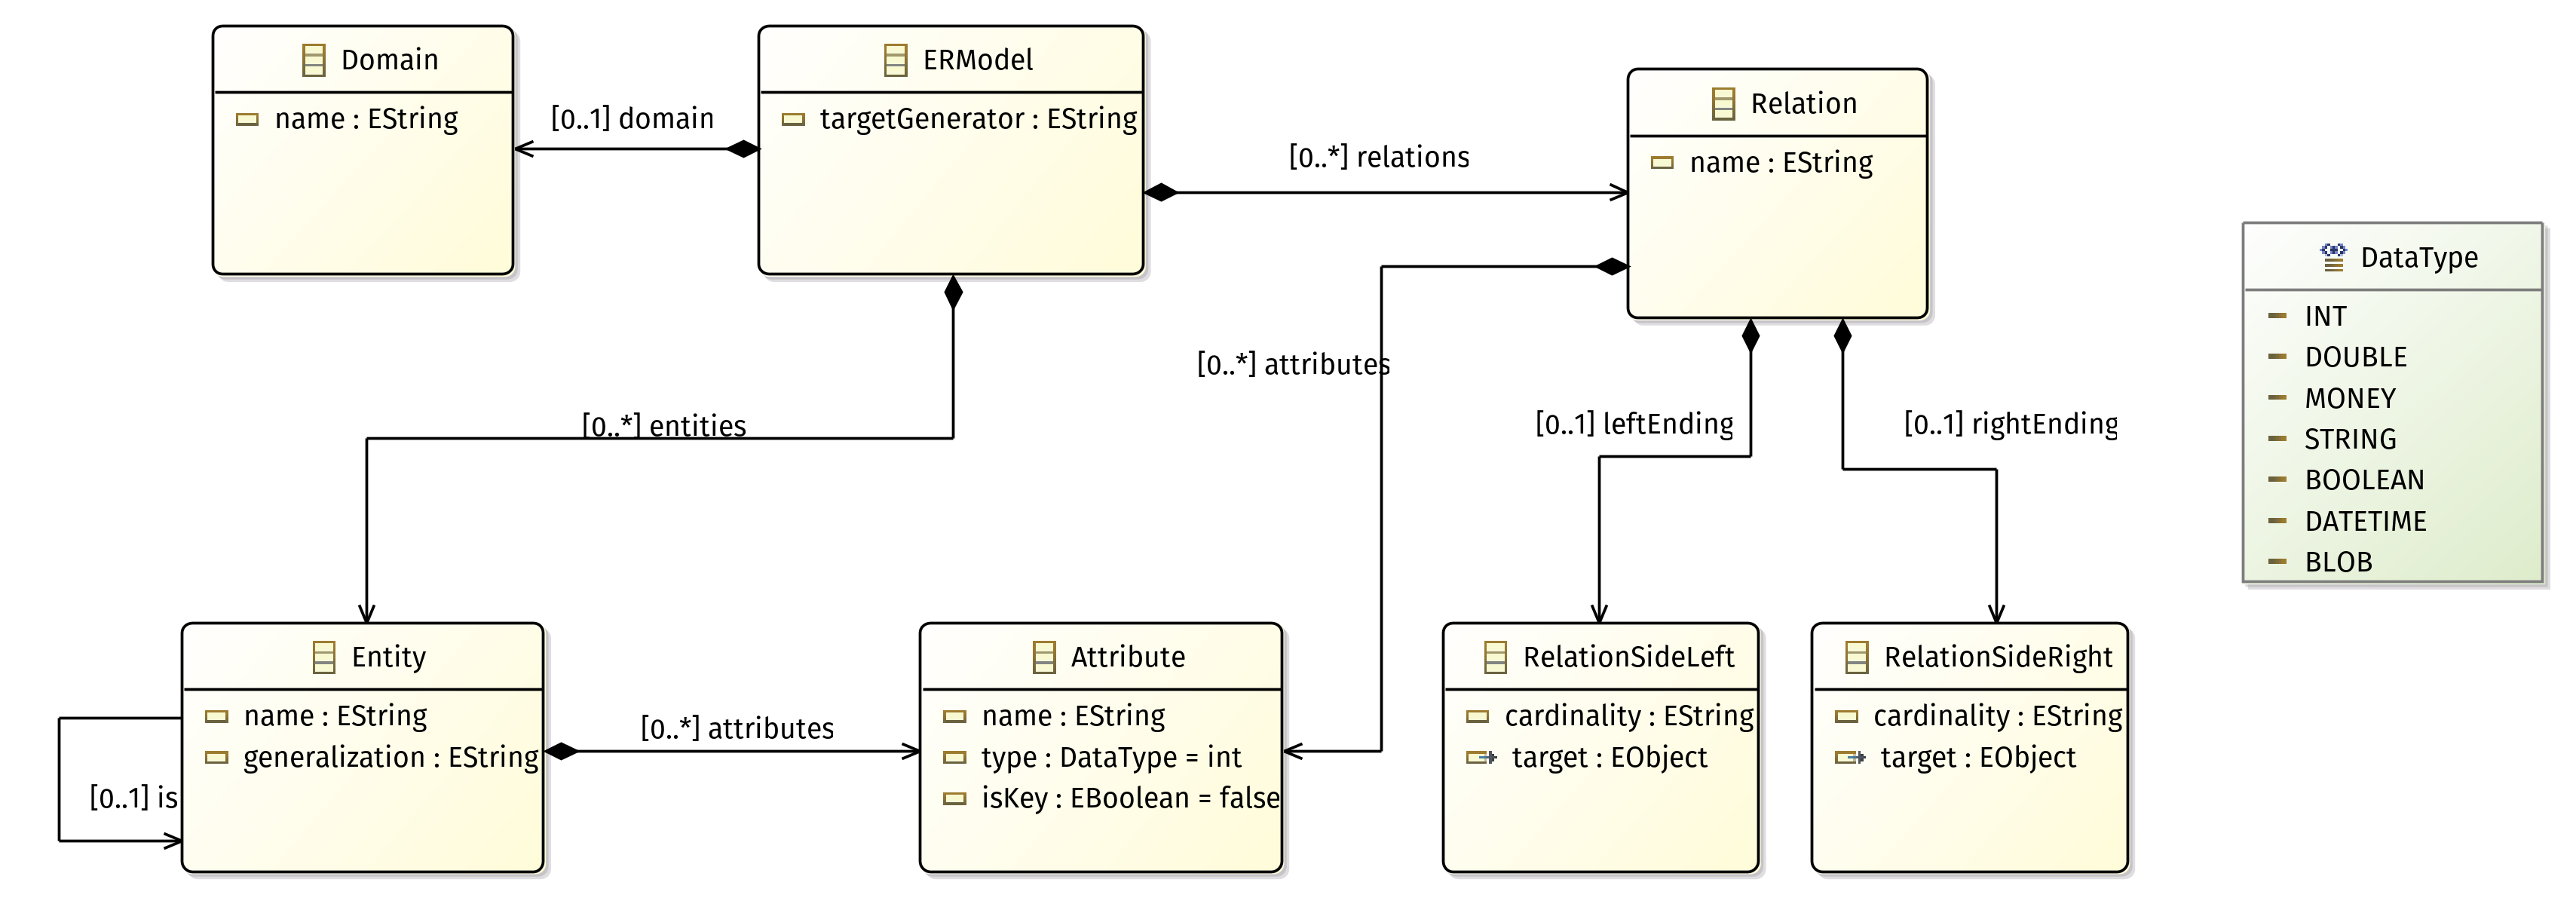
\includegraphics[width=\textwidth]{img/erDsl_class_diagram.png}
    \fonte{Author.}
\end{figure}

% O metamodelo da linguagem é importante na abordagem utilizada no Xtext pois permitiu que a DSL e os geradores sejam construídos separadamente. 
The language metamodel is relevant in the approach used in Xtext as it allowed the DSL and generators to be built separately.

%------------------------------------------------------------------------------
\subsection{Tool Architecture}
%------------------------------------------------------------------------------

% O framework Xtext gera grande parte da infraestrutura para linguagens com base fundamentalmente nas gramáticas definidas. 
% A Figura \ref{fig:arqXtext} fornece uma visão geral em um nível abstrato da arquitetura final da ERtext, arquitetura esta modificada com adição dos geradores SQL e gerador de diagramas com a PlantUML.
The Xtext framework generates much of the infrastructure for languages based fundamentally on defined grammar.
% FALAR DA ENGINE MWE2 ?
Figure \ref{fig:arqERtext} provides an abstract level overview of the final ERtext architecture, which we have modified by adding the SQL generators and diagram generator with PlantUML.
% Figure \ref{fig:arqERtext} provides an abstract level overview of the final ERtext architecture, which has been modified with the addition of SQL generators and diagram generator with PlantUML.

\begin{figure}[!htb]
    \centering
    \caption{ERtext architecture.}
    \label{fig:arqERtext}
    

\tikzset{every picture/.style={line width=0.75pt}} %set default line width to 0.75pt        

\begin{tikzpicture}[x=0.75pt,y=0.75pt,yscale=-1,xscale=1]
%uncomment if require: \path (0,465); %set diagram left start at 0, and has height of 465


%Rounded Rect [id:dp8080613887465731] 
\draw  [fill={rgb, 255:red, 255; green, 255; blue, 255 }  ,fill opacity=1 ] (268.24,22.37) .. controls (268.24,18.97) and (271,16.21) .. (274.4,16.21) -- (365.96,16.21) .. controls (369.36,16.21) and (372.11,18.97) .. (372.11,22.37) -- (372.11,40.84) .. controls (372.11,44.24) and (369.36,47) .. (365.96,47) -- (274.4,47) .. controls (271,47) and (268.24,44.24) .. (268.24,40.84) -- cycle ;
%Rounded Rect [id:dp23877247410758984] 
\draw  [fill={rgb, 255:red, 255; green, 255; blue, 255 }  ,fill opacity=1 ][line width=0.75]  (123.24,92.82) .. controls (123.24,89.42) and (126,86.66) .. (129.4,86.66) -- (220.95,86.66) .. controls (224.36,86.66) and (227.11,89.42) .. (227.11,92.82) -- (227.11,111.3) .. controls (227.11,114.7) and (224.36,117.46) .. (220.95,117.46) -- (129.4,117.46) .. controls (126,117.46) and (123.24,114.7) .. (123.24,111.3) -- cycle ;
%Flowchart: Multidocument [id:dp49717070559395604] 
\draw  [fill={rgb, 255:red, 255; green, 255; blue, 255 }  ,fill opacity=1 ] (158.88,152.12) -- (192.75,152.12) -- (192.75,175.89) .. controls (171.58,175.89) and (175.82,184.46) .. (158.88,178.91) -- cycle ; \draw  [fill={rgb, 255:red, 255; green, 255; blue, 255 }  ,fill opacity=1 ] (154.64,155.72) -- (188.52,155.72) -- (188.52,179.49) .. controls (167.35,179.49) and (171.58,188.06) .. (154.64,182.52) -- cycle ; \draw  [fill={rgb, 255:red, 255; green, 255; blue, 255 }  ,fill opacity=1 ] (150.41,159.32) -- (184.28,159.32) -- (184.28,183.09) .. controls (163.11,183.09) and (167.35,191.66) .. (150.41,186.12) -- cycle ;
%Straight Lines [id:da5642847406466045] 
\draw [fill={rgb, 255:red, 255; green, 255; blue, 255 }  ,fill opacity=1 ]   (153.63,166.47) -- (180.34,166.5) ;
%Straight Lines [id:da9779186616916171] 
\draw [fill={rgb, 255:red, 255; green, 255; blue, 255 }  ,fill opacity=1 ]   (153.63,171.26) -- (180.34,171.28) ;
%Straight Lines [id:da8217185402464098] 
\draw [fill={rgb, 255:red, 255; green, 255; blue, 255 }  ,fill opacity=1 ]   (153.63,176.04) -- (180.34,176.06) ;


%Straight Lines [id:da27204357118531197] 
\draw [fill={rgb, 255:red, 255; green, 255; blue, 255 }  ,fill opacity=1 ][line width=1.5]    (173.18,121.3) -- (173.18,144.06) ;
\draw [shift={(173.18,148.06)}, rotate = 270] [fill={rgb, 255:red, 0; green, 0; blue, 0 }  ][line width=0.08]  [draw opacity=0] (11.61,-5.58) -- (0,0) -- (11.61,5.58) -- cycle    ;
%Rounded Rect [id:dp014713549076222021] 
\draw  [fill={rgb, 255:red, 255; green, 255; blue, 255 }  ,fill opacity=1 ] (261.43,78.98) .. controls (261.43,75.3) and (264.41,72.31) .. (268.09,72.31) -- (371.45,72.31) .. controls (375.13,72.31) and (378.11,75.3) .. (378.11,78.98) -- (378.11,98.98) .. controls (378.11,102.66) and (375.13,105.65) .. (371.45,105.65) -- (268.09,105.65) .. controls (264.41,105.65) and (261.43,102.66) .. (261.43,98.98) -- cycle ;
%Rounded Rect [id:dp8159423215616721] 
\draw  [fill={rgb, 255:red, 255; green, 255; blue, 255 }  ,fill opacity=1 ] (417.72,92.82) .. controls (417.72,89.42) and (420.48,86.66) .. (423.88,86.66) -- (515.44,86.66) .. controls (518.84,86.66) and (521.59,89.42) .. (521.59,92.82) -- (521.59,111.3) .. controls (521.59,114.7) and (518.84,117.46) .. (515.44,117.46) -- (423.88,117.46) .. controls (420.48,117.46) and (417.72,114.7) .. (417.72,111.3) -- cycle ;
%Flowchart: Multidocument [id:dp814245162277164] 
\draw  [fill={rgb, 255:red, 255; green, 255; blue, 255 }  ,fill opacity=1 ] (454.96,152.12) -- (488.83,152.12) -- (488.83,175.89) .. controls (467.66,175.89) and (471.89,184.46) .. (454.96,178.91) -- cycle ; \draw  [fill={rgb, 255:red, 255; green, 255; blue, 255 }  ,fill opacity=1 ] (450.72,155.72) -- (484.6,155.72) -- (484.6,179.49) .. controls (463.43,179.49) and (467.66,188.06) .. (450.72,182.52) -- cycle ; \draw  [fill={rgb, 255:red, 255; green, 255; blue, 255 }  ,fill opacity=1 ] (446.49,159.32) -- (480.36,159.32) -- (480.36,183.09) .. controls (459.19,183.09) and (463.43,191.66) .. (446.49,186.12) -- cycle ;
%Straight Lines [id:da659202853659377] 
\draw [fill={rgb, 255:red, 255; green, 255; blue, 255 }  ,fill opacity=1 ]   (449.97,166.04) -- (476.69,166.06) ;
%Straight Lines [id:da8271632436642871] 
\draw [fill={rgb, 255:red, 255; green, 255; blue, 255 }  ,fill opacity=1 ]   (449.97,170.82) -- (476.69,170.85) ;
%Straight Lines [id:da22701123408508272] 
\draw [fill={rgb, 255:red, 255; green, 255; blue, 255 }  ,fill opacity=1 ]   (449.97,175.61) -- (476.69,175.63) ;


%Straight Lines [id:da6612735011438882] 
\draw [fill={rgb, 255:red, 255; green, 255; blue, 255 }  ,fill opacity=1 ][line width=1.5]    (470.86,124.65) -- (470.86,147.4) ;
\draw [shift={(470.86,120.65)}, rotate = 90] [fill={rgb, 255:red, 0; green, 0; blue, 0 }  ][line width=0.08]  [draw opacity=0] (11.61,-5.58) -- (0,0) -- (11.61,5.58) -- cycle    ;
%Rounded Rect [id:dp9641259565957541] 
\draw  [fill={rgb, 255:red, 255; green, 255; blue, 255 }  ,fill opacity=1 ] (268.24,145.89) .. controls (268.24,142.48) and (271,139.73) .. (274.4,139.73) -- (365.96,139.73) .. controls (369.36,139.73) and (372.11,142.48) .. (372.11,145.89) -- (372.11,164.36) .. controls (372.11,167.76) and (369.36,170.52) .. (365.96,170.52) -- (274.4,170.52) .. controls (271,170.52) and (268.24,167.76) .. (268.24,164.36) -- cycle ;
%Straight Lines [id:da4555835119587406] 
\draw [fill={rgb, 255:red, 255; green, 255; blue, 255 }  ,fill opacity=1 ][line width=1.5]    (320.18,48.89) -- (320.18,66.42) ;
\draw [shift={(320.18,70.42)}, rotate = 270] [fill={rgb, 255:red, 0; green, 0; blue, 0 }  ][line width=0.08]  [draw opacity=0] (11.61,-5.58) -- (0,0) -- (11.61,5.58) -- cycle    ;
%Straight Lines [id:da2586670416419199] 
\draw [fill={rgb, 255:red, 255; green, 255; blue, 255 }  ,fill opacity=1 ][line width=1.5]    (320.18,107.78) -- (320.18,131.88) ;
\draw [shift={(320.18,135.88)}, rotate = 270] [fill={rgb, 255:red, 0; green, 0; blue, 0 }  ][line width=0.08]  [draw opacity=0] (11.61,-5.58) -- (0,0) -- (11.61,5.58) -- cycle    ;
%Straight Lines [id:da2552674310073062] 
\draw [fill={rgb, 255:red, 255; green, 255; blue, 255 }  ,fill opacity=1 ][line width=1.5]    (259.32,90.59) -- (234.04,102.77) ;
\draw [shift={(230.43,104.51)}, rotate = 334.28] [fill={rgb, 255:red, 0; green, 0; blue, 0 }  ][line width=0.08]  [draw opacity=0] (11.61,-5.58) -- (0,0) -- (11.61,5.58) -- cycle    ;
%Straight Lines [id:da29550662771480396] 
\draw [fill={rgb, 255:red, 255; green, 255; blue, 255 }  ,fill opacity=1 ][line width=1.5]    (410.34,102.31) -- (380.52,90.81) ;
\draw [shift={(414.07,103.76)}, rotate = 201.11] [fill={rgb, 255:red, 0; green, 0; blue, 0 }  ][line width=0.08]  [draw opacity=0] (11.61,-5.58) -- (0,0) -- (11.61,5.58) -- cycle    ;
%Straight Lines [id:da3280771928101003] 
\draw [fill={rgb, 255:red, 255; green, 255; blue, 255 }  ,fill opacity=1 ][line width=1.5]    (199.15,166.77) -- (259.22,157.13) ;
\draw [shift={(263.17,156.5)}, rotate = 530.89] [fill={rgb, 255:red, 0; green, 0; blue, 0 }  ][line width=0.08]  [draw opacity=0] (11.61,-5.58) -- (0,0) -- (11.61,5.58) -- cycle    ;
%Straight Lines [id:da9478402467031726] 
\draw [fill={rgb, 255:red, 255; green, 255; blue, 255 }  ,fill opacity=1 ][line width=1.5]    (379.03,157.51) -- (436.63,170.02) ;
\draw [shift={(440.54,170.87)}, rotate = 192.26] [fill={rgb, 255:red, 0; green, 0; blue, 0 }  ][line width=0.08]  [draw opacity=0] (11.61,-5.58) -- (0,0) -- (11.61,5.58) -- cycle    ;
%Flowchart: Direct Access Storage [id:dp7657317583515377] 
\draw  [fill={rgb, 255:red, 255; green, 255; blue, 255 }  ,fill opacity=1 ] (331.43,264.99) -- (255.92,264.99) .. controls (244.69,264.99) and (235.59,257.2) .. (235.59,247.6) .. controls (235.59,238) and (244.69,230.21) .. (255.92,230.21) -- (331.43,230.21)(351.75,247.6) .. controls (351.75,257.2) and (342.65,264.99) .. (331.43,264.99) .. controls (320.2,264.99) and (311.1,257.2) .. (311.1,247.6) .. controls (311.1,238) and (320.2,230.21) .. (331.43,230.21) .. controls (342.65,230.21) and (351.75,238) .. (351.75,247.6) ;
%Straight Lines [id:da100480350897858] 
\draw [fill={rgb, 255:red, 255; green, 255; blue, 255 }  ,fill opacity=1 ][line width=1.5]    (437.65,178.79) -- (316.46,224.67) ;
\draw [shift={(312.72,226.08)}, rotate = 339.27] [fill={rgb, 255:red, 0; green, 0; blue, 0 }  ][line width=0.08]  [draw opacity=0] (11.61,-5.58) -- (0,0) -- (11.61,5.58) -- cycle    ;
%Flowchart: Multidocument [id:dp5253239734010293] 
\draw  [fill={rgb, 255:red, 255; green, 255; blue, 255 }  ,fill opacity=1 ] (297.41,339.12) -- (331.29,339.12) -- (331.29,362.88) .. controls (310.11,362.88) and (314.35,371.45) .. (297.41,365.91) -- cycle ; \draw  [fill={rgb, 255:red, 255; green, 255; blue, 255 }  ,fill opacity=1 ] (293.18,342.72) -- (327.05,342.72) -- (327.05,366.48) .. controls (305.88,366.48) and (310.11,375.05) .. (293.18,369.51) -- cycle ; \draw  [fill={rgb, 255:red, 255; green, 255; blue, 255 }  ,fill opacity=1 ] (288.94,346.32) -- (322.82,346.32) -- (322.82,370.08) .. controls (301.65,370.08) and (305.88,378.66) .. (288.94,373.11) -- cycle ;
%Straight Lines [id:da29635223798470123] 
\draw [fill={rgb, 255:red, 255; green, 255; blue, 255 }  ,fill opacity=1 ]   (292.43,353.03) -- (319.14,353.05) ;
%Straight Lines [id:da45709195099870326] 
\draw [fill={rgb, 255:red, 255; green, 255; blue, 255 }  ,fill opacity=1 ]   (292.43,357.82) -- (319.14,357.84) ;
%Straight Lines [id:da9397926099052756] 
\draw [fill={rgb, 255:red, 255; green, 255; blue, 255 }  ,fill opacity=1 ]   (292.43,362.6) -- (319.14,362.62) ;




%Straight Lines [id:da10826901476686546] 
\draw [fill={rgb, 255:red, 255; green, 255; blue, 255 }  ,fill opacity=1 ][line width=1.5]    (302.13,270.64) -- (307.34,331.21) ;
\draw [shift={(307.68,335.2)}, rotate = 265.08] [fill={rgb, 255:red, 0; green, 0; blue, 0 }  ][line width=0.08]  [draw opacity=0] (11.61,-5.58) -- (0,0) -- (11.61,5.58) -- cycle    ;
%Flowchart: Sequential Access Storage [id:dp3007368871754543] 
\draw  [fill={rgb, 255:red, 255; green, 255; blue, 255 }  ,fill opacity=1 ] (409.6,231.24) .. controls (409.6,220.96) and (396.69,212.63) .. (380.76,212.63) .. controls (364.84,212.63) and (351.93,220.96) .. (351.93,231.24) .. controls (351.93,236.31) and (355.07,240.9) .. (360.17,244.26) -- (351.93,244.26) -- (351.93,249.84) -- (380.76,249.84) .. controls (396.69,249.84) and (409.6,241.51) .. (409.6,231.24) -- cycle ;
%Shape: Rectangle [id:dp03278310257286665] 
\draw   (141.03,319.87) -- (215.03,319.87) -- (215.03,359.87) -- (141.03,359.87) -- cycle ;
%Shape: Rectangle [id:dp9445861445312367] 
\draw   (145.83,326.14) -- (163.55,326.14) -- (163.55,335.52) -- (145.83,335.52) -- cycle ;
%Shape: Rectangle [id:dp035309426832852875] 
\draw   (193.63,335.34) -- (211.34,335.34) -- (211.34,344.72) -- (193.63,344.72) -- cycle ;
%Shape: Rectangle [id:dp0682098761538128] 
\draw   (155.23,346.54) -- (172.94,346.54) -- (172.94,355.92) -- (155.23,355.92) -- cycle ;
%Straight Lines [id:da09626722375251995] 
\draw    (172.65,350.78) -- (193.32,342.78) ;
%Straight Lines [id:da41470258123307224] 
\draw    (163.65,330.44) -- (193.32,338.78) ;


%Straight Lines [id:da24414024149042923] 
\draw [fill={rgb, 255:red, 255; green, 255; blue, 255 }  ,fill opacity=1 ][line width=1.5]    (276.13,271.19) -- (207.1,313.12) ;
\draw [shift={(203.68,315.2)}, rotate = 328.72] [fill={rgb, 255:red, 0; green, 0; blue, 0 }  ][line width=0.08]  [draw opacity=0] (11.61,-5.58) -- (0,0) -- (11.61,5.58) -- cycle    ;
%Flowchart: Multidocument [id:dp9410827405643849] 
\draw  [fill={rgb, 255:red, 255; green, 255; blue, 255 }  ,fill opacity=1 ] (407.36,319.12) -- (441.24,319.12) -- (441.24,342.88) .. controls (420.07,342.88) and (424.3,351.45) .. (407.36,345.91) -- cycle ; \draw  [fill={rgb, 255:red, 255; green, 255; blue, 255 }  ,fill opacity=1 ] (403.13,322.72) -- (437.01,322.72) -- (437.01,346.48) .. controls (415.83,346.48) and (420.07,355.05) .. (403.13,349.51) -- cycle ; \draw  [fill={rgb, 255:red, 255; green, 255; blue, 255 }  ,fill opacity=1 ] (398.89,326.32) -- (432.77,326.32) -- (432.77,350.08) .. controls (411.6,350.08) and (415.83,358.66) .. (398.89,353.11) -- cycle ;
%Straight Lines [id:da31801059922861796] 
\draw [fill={rgb, 255:red, 255; green, 255; blue, 255 }  ,fill opacity=1 ]   (402.38,333.03) -- (429.1,333.05) ;
%Straight Lines [id:da19940799584772861] 
\draw [fill={rgb, 255:red, 255; green, 255; blue, 255 }  ,fill opacity=1 ]   (402.38,337.82) -- (429.1,337.84) ;
%Straight Lines [id:da720164043002747] 
\draw [fill={rgb, 255:red, 255; green, 255; blue, 255 }  ,fill opacity=1 ]   (402.38,342.6) -- (429.1,342.62) ;




%Straight Lines [id:da4341747356667731] 
\draw [fill={rgb, 255:red, 255; green, 255; blue, 255 }  ,fill opacity=1 ][line width=1.5]    (337.96,267.69) -- (391.64,313.6) ;
\draw [shift={(394.68,316.2)}, rotate = 220.53] [fill={rgb, 255:red, 0; green, 0; blue, 0 }  ][line width=0.08]  [draw opacity=0] (11.61,-5.58) -- (0,0) -- (11.61,5.58) -- cycle    ;



% Text Node
\draw (175.18,102.06) node   [align=left] {Editor};
% Text Node
\draw (469.66,102.06) node   [align=left] {Ecore};
% Text Node
\draw (320.18,155.12) node   [align=left] {Parser};
% Text Node
\draw (320.18,31.6) node  [font=\normalsize] [align=left] {Grammar};
% Text Node
\draw (168.54,201.99) node   [align=left] {{\scriptsize Conceptual Model}};
% Text Node
\draw (463.03,201.99) node   [align=left] {{\scriptsize EMF Model}};
% Text Node
\draw (275.76,247.14) node  [font=\footnotesize] [align=left] {\begin{minipage}[lt]{39.43pt}\setlength\topsep{0pt}
\begin{center}
Generator
\end{center}

\end{minipage}};
% Text Node
\draw (380.24,230.37) node  [font=\scriptsize] [align=left] {\begin{minipage}[lt]{20.96pt}\setlength\topsep{0pt}
\begin{center}
Rules
\end{center}

\end{minipage}};
% Text Node
\draw (136.8,126.16) node [anchor=north west][inner sep=0.75pt]  [font=\scriptsize,color={rgb, 255:red, 74; green, 74; blue, 74 }  ,opacity=1 ] [align=left] {edit};
% Text Node
\draw (207,146.18) node [anchor=north west][inner sep=0.75pt]  [font=\scriptsize,color={rgb, 255:red, 74; green, 74; blue, 74 }  ,opacity=1 ] [align=left] {parse};
% Text Node
\draw (397,146.18) node [anchor=north west][inner sep=0.75pt]  [font=\scriptsize,color={rgb, 255:red, 74; green, 74; blue, 74 }  ,opacity=1 ] [align=left] {create};
% Text Node
\draw (487.4,130.21) node [anchor=north west][inner sep=0.75pt]  [font=\scriptsize,color={rgb, 255:red, 74; green, 74; blue, 74 }  ,opacity=1 ] [align=left] {instance};
% Text Node
\draw (316,188.69) node [anchor=north west][inner sep=0.75pt]  [font=\scriptsize,color={rgb, 255:red, 74; green, 74; blue, 74 }  ,opacity=1 ] [align=left] {handled};
% Text Node
\draw (502.4,145.21) node [anchor=north west][inner sep=0.75pt]  [font=\scriptsize,color={rgb, 255:red, 74; green, 74; blue, 74 }  ,opacity=1 ] [align=left] {of};
% Text Node
\draw (319.77,88.98) node  [font=\footnotesize] [align=left] {Xtext Generator};
% Text Node
\draw (168.54,217.99) node   [align=left] {{\scriptsize (DSL Model)}};
% Text Node
\draw (204,268.3) node [anchor=north west][inner sep=0.75pt]  [font=\scriptsize,color={rgb, 255:red, 74; green, 74; blue, 74 }  ,opacity=1 ] [align=left] {convert};
% Text Node
\draw (213,282.3) node [anchor=north west][inner sep=0.75pt]  [font=\scriptsize,color={rgb, 255:red, 74; green, 74; blue, 74 }  ,opacity=1 ] [align=left] {into};
% Text Node
\draw (305.48,385.98) node   [align=left] {{\scriptsize Logical Model}};
% Text Node
\draw (415.43,365.98) node   [align=left] {{\scriptsize Physical Model}};
% Text Node
\draw (284.48,392.91) node [anchor=north west][inner sep=0.75pt]   [align=left] {{\tiny \textcolor[rgb]{0.5,0.5,0.5}{\textbf{(HTML)}}}};
% Text Node
\draw (360.43,372.91) node [anchor=north west][inner sep=0.75pt]   [align=left] {{\tiny \textcolor[rgb]{0.5,0.5,0.5}{\textbf{(PostgreSQL, MySQL)}}}};
% Text Node
\draw (147.53,380.15) node [anchor=north west][inner sep=0.75pt]   [align=left] {{\tiny \textcolor[rgb]{0.5,0.5,0.5}{\textbf{(PlantUML)}}}};
% Text Node
\draw (178.03,371.89) node   [align=left] {{\scriptsize Conceptual Diagram}};
% Text Node
\draw (269.5,303.8) node [anchor=north west][inner sep=0.75pt]  [font=\scriptsize,color={rgb, 255:red, 74; green, 74; blue, 74 }  ,opacity=1 ] [align=left] {into};
% Text Node
\draw (260.5,289.8) node [anchor=north west][inner sep=0.75pt]  [font=\scriptsize,color={rgb, 255:red, 74; green, 74; blue, 74 }  ,opacity=1 ] [align=left] {convert};
% Text Node
\draw (330,303.8) node [anchor=north west][inner sep=0.75pt]  [font=\scriptsize,color={rgb, 255:red, 74; green, 74; blue, 74 }  ,opacity=1 ] [align=left] {into};
% Text Node
\draw (321,289.8) node [anchor=north west][inner sep=0.75pt]  [font=\scriptsize,color={rgb, 255:red, 74; green, 74; blue, 74 }  ,opacity=1 ] [align=left] {convert};


\end{tikzpicture}

    \fonte{Author.}
\end{figure}

% Dizemos que o Xtext gera grande parte, e não completamente, pois existem diversos aspectos que devem ser implementados de acordo com os requisitos e objetivos da linguagem.
% Por exemplo, toda a parte de validação com com base no escopo, marcação e feedback de erros, sugestão de trechos de código, criação de templates, e wizards de criação de projetos e arquivos específicos para a linguagem precisam e foram implementados manualmente.
We say that Xtext generates a majority part, but not entirely, as several aspects must be implemented according to the requirements and objectives of the language.
% For example, all of the scope-based validation, bug marking and feedback, snippet suggestion, template creation, and language-specific project and file creation wizards need and have been implemented manually.
For example, we have manually needed and implemented the following aspects, all of the scope-based validation, bug marking and feedback, snippet suggestion, template creation, and language-specific project and file creation wizards.

%------------------------------------------------------------------------------
\subsection{Stable Version}
%------------------------------------------------------------------------------

% O código fonte da versão estável da ferramenta de modelagem produzida está disponível em um repositório público no GitHub\footnote{Repositório: \url{https://github.com/ProjetoDSL/ERDSL}}.
% Esta versão será irá para a última avaliação experimental que será planejada para avaliar não só a \ac{dsl} como também os artefatos que podem ser produzidos por ela, bem como sua usabilidade.
% A Figura \ref{fig:stableVersion} apresenta um fragmento visual da ferramenta em uso.
The source code of the stable version of the produced modeling tool is available in a public repository on GitHub\footnote{Repository: \url{https://github.com/ProjetoDSL/ERDSL}}.
This version will go to the last experimental evaluation which will be designed to evaluate not only the \ac{dsl} but also the artifacts that can be produced by it, as well as its usability.
Figure \ref{fig:stableVersion} presents a visual fragment of the tool in use.

\begin{figure} [!htb]
    \centering
    \caption{ERtext tool stable version.}
    \label{fig:stableVersion}
    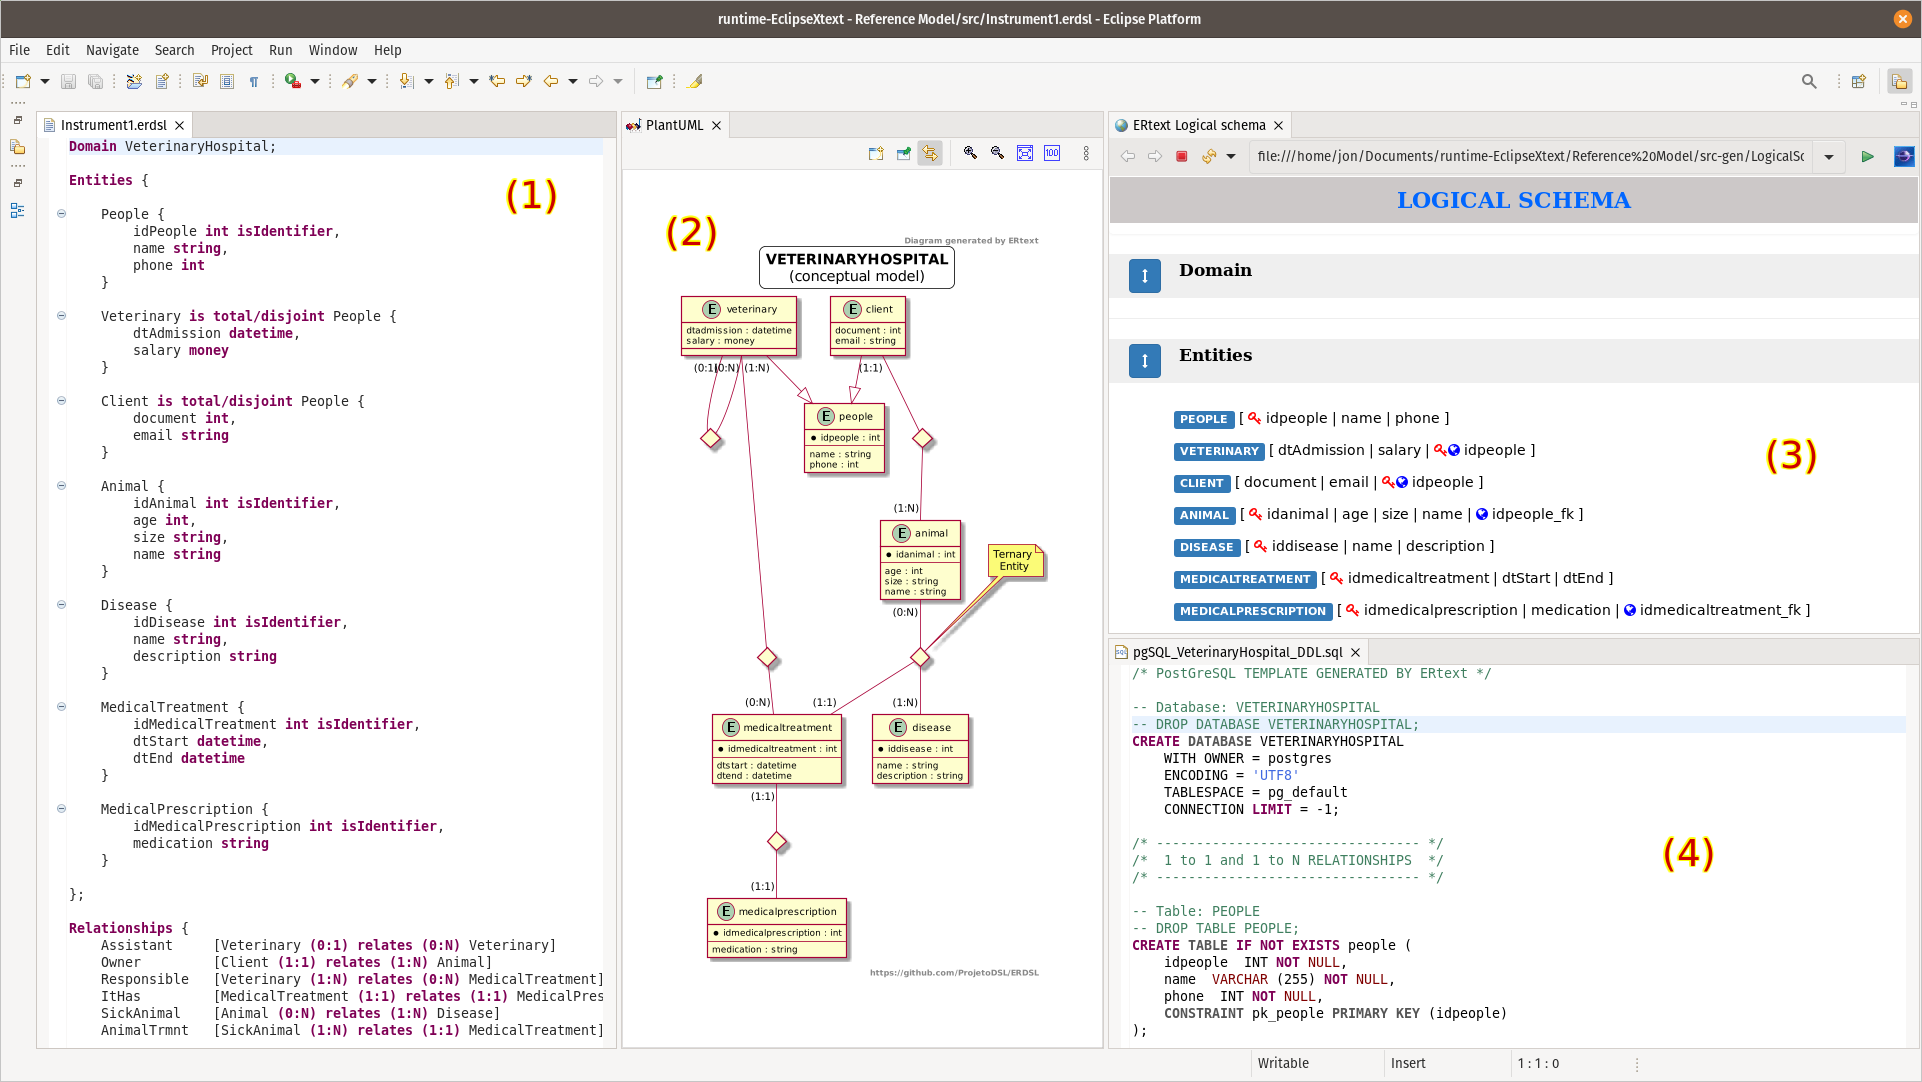
\includegraphics[width=1\textwidth]{img/ToolOverview2.png}
    \fonte{Author.}
\end{figure}

% A legenda (1) na figura demonstra o editor com um modelo descrito na DSL implementada. A legenda (2) apresenta uma representação gráfica (diagrama) utilizando a integração com PlantUML. 
% Para isto o modelo é transformado da nossa DSL para a notação necessária para o PlantUML gerar o diagrama utilizando bibliotecas do Graphviz.
% A legenda (3) mostra o modelo transformado para uma notação lógica, já resolvendo as relações, ou seja, as chaves primárias e estrangeiras.
% Finalmente, na legenda (4) apresentamos o código SQL DDL gerada para o \ac{dbms} PostgreSQL 
The caption (1) in the figure demonstrates the editor with a model described in the implemented \ac{dsl} notation.
Caption (2) presents a graphical representation (diagram) using the integration with PlantUML.
For this, the model is transformed from our \ac{dsl} to the necessary notation for PlantUML to generate the diagram using Graphviz libraries.
Caption (3) shows the model transformed to a logical notation, already solving the relations, \textit{i.e.} the primary and foreign keys.
Finally, in caption (4) we present the generated \ac{sql} \ac{ddl} code for \ac{dbms} PostgreSQL.

% Para as tranformações dos modelos foi avaliado as opções de regras de transformações descritas por~\cite{Heuser:2009}.
% Em relação aos relacionamentos do tipo 1:1 adotou-se a estratégia de adição de coluna para os três casos possíveis.
% Para os relacionamentos 1:N seguiu-se a mesma premissa de transformação para os quatro (4) casos possíveis.
% Já para a transformação de relacionamentos N:N optou-se pela única regra de transformação recomendada, ou seja, a regra de criação de tabelas próprias para os três (3) casos.
For the transformations of the models, we have evaluated the transformation rule options described by~\cite{Heuser:2009}.
Regarding 1:1 type relationships, we have adopted the column addition strategy for the three (3) possible cases.
For the 1:N relationships, we have followed the same transformation premise for the four (4) possible cases.
For the transformation of N:N relationships, we have chosen the only recommended transformation rule, \textit{i.e.} the rule for creating own tables for the three (3) cases.

% Basicamente durante a atividade de modelagem um arquivo de texto plano é criado com a extensão da linguagem (.erdsl) no sistema que está rodando a ferramenta.
% A cada vez que este arquivo é salvo um modelo Ecore é criado ou atualizado para então ser chamado aos geradores que lidam com os artefatos que devem ser criados.
% Isto acontece através da interface \ texttt {IFileSystemAccess2} que oferece o meio para percorrer o modelo criado e aplicar como regras de transformação em um cenário standalone.
% Esta interface oferece uma abstração para operações no sistema de arquivos, possibilitando o mapeamento de caminho lógico (artefato de saída). 
% Esta interface compõe todas as interfaces de extensão para \ texttt {IFileSystemAccess} com outras melhorias implementadas diretamente.
Basically, during the modeling activity a plain text file is created with the language extension (.erdsl) on the system running the tool.
Each time this file is saved, an Ecore model is created or updated and then called to the generators that handle the artifacts that must be created.
It happens through the \texttt {IFileSystemAccess2} interface that provides the means to iterate through the created model and apply as transformation rules in a standalone scenario.
This interface provides an abstraction for file system operations, enabling logical path mapping (output artifact).
This interface composes all the extension interfaces for \texttt {IFileSystemAccess} with other improvements implemented.



% \begin{figure}[!htb]
%     \centering
%     \caption{Transformation rules adopted.}
%     \label{fig:transformationRules}
%     

\tikzset{every picture/.style={line width=0.75pt}} %set default line width to 0.75pt        

\begin{tikzpicture}[x=0.75pt,y=0.75pt,yscale=-1,xscale=1]
%uncomment if require: \path (0,499); %set diagram left start at 0, and has height of 499

%Shape: Star [id:dp905069961258552] 
\draw   (18.05,469.49) -- (21.63,473.53) -- (29.64,474.18) -- (23.84,477.33) -- (25.21,481.76) -- (18.05,479.67) -- (10.88,481.76) -- (12.25,477.33) -- (6.46,474.18) -- (14.47,473.53) -- cycle ;
%Flowchart: Summing Junction [id:dp5670844386539957] 
\draw   (335.82,475.68) .. controls (335.82,471.6) and (339.21,468.29) .. (343.4,468.29) .. controls (347.59,468.29) and (350.98,471.6) .. (350.98,475.68) .. controls (350.98,479.75) and (347.59,483.06) .. (343.4,483.06) .. controls (339.21,483.06) and (335.82,479.75) .. (335.82,475.68) -- cycle ; \draw   (338.04,470.45) -- (348.76,480.9) ; \draw   (348.76,470.45) -- (338.04,480.9) ;
%Shape: Triangle [id:dp8755221528505448] 
\draw   (202.36,467.09) -- (214.95,481.1) -- (189.78,481.1) -- cycle ;
%Shape: Diamond [id:dp15610691613574645] 
\draw   (108.29,66.95) -- (144.12,76.62) -- (108.29,86.29) -- (72.46,76.62) -- cycle ;
%Straight Lines [id:da1548262316328981] 
\draw    (72.46,76.62) -- (45.55,76.61) ;
%Straight Lines [id:da34976069343568916] 
\draw    (171.03,76.63) -- (144.12,76.62) ;


%Shape: Rectangle [id:dp9438218872468358] 
\draw   (4.84,5.4) -- (213.33,5.4) -- (213.33,162.47) -- (4.84,162.47) -- cycle ;
%Shape: Diamond [id:dp2599956034792046] 
\draw   (108.29,102.1) -- (144.12,111.77) -- (108.29,121.43) -- (72.46,111.77) -- cycle ;
%Straight Lines [id:da5197763190540488] 
\draw    (72.46,111.77) -- (45.55,111.75) ;
%Straight Lines [id:da8940402532777019] 
\draw    (171.03,111.78) -- (144.12,111.77) ;


%Shape: Diamond [id:dp7953044653471437] 
\draw   (108.29,137.24) -- (144.12,146.91) -- (108.29,156.58) -- (72.46,146.91) -- cycle ;
%Straight Lines [id:da20949304709496497] 
\draw    (72.46,146.91) -- (45.55,146.9) ;
%Straight Lines [id:da34589572563098536] 
\draw    (171.03,146.92) -- (144.12,146.91) ;


%Straight Lines [id:da22563177204480978] 
\draw    (5.11,39.21) -- (212.78,39.79) ;
%Straight Lines [id:da6727878622034686] 
\draw    (5.38,56.79) -- (212.78,57.1) ;
%Straight Lines [id:da03418802907814289] 
\draw    (212.78,57.1) -- (448.88,57.4) ;
%Straight Lines [id:da9489243894366923] 
\draw    (212.78,39.79) -- (449.15,40.36) ;
%Shape: Rectangle [id:dp7744485792611493] 
\draw   (213.33,5.4) -- (449.14,5.4) -- (449.14,162.47) -- (213.33,162.47) -- cycle ;
%Straight Lines [id:da1104964129518442] 
\draw    (273.52,39.45) -- (273.52,162.59) ;
%Straight Lines [id:da5208240902682426] 
\draw    (368.51,39.09) -- (368.51,162.23) ;
%Shape: Star [id:dp5079293847310995] 
\draw   (319.96,192.53) -- (323.54,196.57) -- (331.55,197.22) -- (325.75,200.36) -- (327.12,204.8) -- (319.96,202.7) -- (312.8,204.8) -- (314.16,200.36) -- (308.37,197.22) -- (316.38,196.57) -- cycle ;
%Shape: Triangle [id:dp4199850954698714] 
\draw   (245.13,192.42) -- (257.72,206.43) -- (232.54,206.43) -- cycle ;
%Flowchart: Summing Junction [id:dp2114922561352448] 
\draw   (400.87,200.8) .. controls (400.87,196.72) and (404.27,193.42) .. (408.45,193.42) .. controls (412.64,193.42) and (416.04,196.72) .. (416.04,200.8) .. controls (416.04,204.88) and (412.64,208.19) .. (408.45,208.19) .. controls (404.27,208.19) and (400.87,204.88) .. (400.87,200.8) -- cycle ; \draw   (403.09,195.58) -- (413.82,206.02) ; \draw   (413.82,195.58) -- (403.09,206.02) ;
%Shape: Star [id:dp051836092901429875] 
\draw   (320.16,70.15) -- (323.74,74.19) -- (331.75,74.84) -- (325.95,77.98) -- (327.32,82.42) -- (320.16,80.32) -- (312.99,82.42) -- (314.36,77.98) -- (308.57,74.84) -- (316.58,74.19) -- cycle ;
%Shape: Triangle [id:dp16503862399573688] 
\draw   (320.16,105.65) -- (332.74,119.66) -- (307.57,119.66) -- cycle ;
%Shape: Triangle [id:dp2109056154155149] 
\draw   (320.16,140.26) -- (332.74,154.27) -- (307.57,154.27) -- cycle ;
%Shape: Triangle [id:dp6106295252529019] 
\draw   (243.42,69.71) -- (256.01,83.72) -- (230.84,83.72) -- cycle ;
%Flowchart: Summing Junction [id:dp7641214677961137] 
\draw   (235.84,112.27) .. controls (235.84,108.19) and (239.23,104.89) .. (243.42,104.89) .. controls (247.61,104.89) and (251,108.19) .. (251,112.27) .. controls (251,116.35) and (247.61,119.66) .. (243.42,119.66) .. controls (239.23,119.66) and (235.84,116.35) .. (235.84,112.27) -- cycle ; \draw   (238.06,107.05) -- (248.78,117.5) ; \draw   (248.78,107.05) -- (238.06,117.5) ;
%Flowchart: Summing Junction [id:dp22623131635410432] 
\draw   (235.84,146.89) .. controls (235.84,142.81) and (239.23,139.5) .. (243.42,139.5) .. controls (247.61,139.5) and (251,142.81) .. (251,146.89) .. controls (251,150.96) and (247.61,154.27) .. (243.42,154.27) .. controls (239.23,154.27) and (235.84,150.96) .. (235.84,146.89) -- cycle ; \draw   (238.06,141.66) -- (248.78,152.11) ; \draw   (248.78,141.66) -- (238.06,152.11) ;
%Flowchart: Summing Junction [id:dp8111950400823971] 
\draw   (402.24,76.33) .. controls (402.24,72.25) and (405.63,68.94) .. (409.82,68.94) .. controls (414.01,68.94) and (417.4,72.25) .. (417.4,76.33) .. controls (417.4,80.41) and (414.01,83.72) .. (409.82,83.72) .. controls (405.63,83.72) and (402.24,80.41) .. (402.24,76.33) -- cycle ; \draw   (404.46,71.11) -- (415.18,81.55) ; \draw   (415.18,71.11) -- (404.46,81.55) ;
%Shape: Star [id:dp8714716991158269] 
\draw   (409.82,106.09) -- (413.4,110.13) -- (421.41,110.78) -- (415.62,113.92) -- (416.98,118.36) -- (409.82,116.27) -- (402.66,118.36) -- (404.03,113.92) -- (398.23,110.78) -- (406.24,110.13) -- cycle ;
%Shape: Star [id:dp9624342328821995] 
\draw   (409.82,140.7) -- (413.4,144.74) -- (421.41,145.39) -- (415.62,148.54) -- (416.98,152.98) -- (409.82,150.88) -- (402.66,152.98) -- (404.03,148.54) -- (398.23,145.39) -- (406.24,144.74) -- cycle ;
%Shape: Rectangle [id:dp04619740593055166] 
\draw   (4.84,162.47) -- (213.33,162.47) -- (213.33,319.53) -- (4.84,319.53) -- cycle ;
%Shape: Diamond [id:dp27789691615521184] 
\draw   (108.57,190.76) -- (144.39,200.43) -- (108.57,210.09) -- (72.74,200.43) -- cycle ;
%Straight Lines [id:da6441724439769754] 
\draw    (72.74,200.43) -- (45.83,200.41) ;
%Straight Lines [id:da38653260527553623] 
\draw    (171.31,200.44) -- (144.39,200.43) ;


%Shape: Diamond [id:dp2739495911529186] 
\draw   (109.25,224.84) -- (145.08,234.51) -- (109.25,244.17) -- (73.42,234.51) -- cycle ;
%Straight Lines [id:da7680368197813587] 
\draw    (73.42,234.51) -- (46.51,234.49) ;
%Straight Lines [id:da16254742962238433] 
\draw    (171.99,234.52) -- (145.08,234.51) ;


%Shape: Diamond [id:dp37713417833040097] 
\draw   (109.25,258.92) -- (145.08,268.59) -- (109.25,278.25) -- (73.42,268.59) -- cycle ;
%Straight Lines [id:da7776121131254392] 
\draw    (73.42,268.59) -- (46.51,268.57) ;
%Straight Lines [id:da010163980070524659] 
\draw    (171.99,268.6) -- (145.08,268.59) ;


%Straight Lines [id:da17800868812349258] 
\draw    (5.38,182.59) -- (212.78,182.9) ;
%Shape: Diamond [id:dp5731700485298001] 
\draw   (108.57,293) -- (144.39,302.67) -- (108.57,312.33) -- (72.74,302.67) -- cycle ;
%Straight Lines [id:da44119921508225857] 
\draw    (72.74,302.67) -- (45.83,302.65) ;
%Straight Lines [id:da0629754002847982] 
\draw    (171.31,302.68) -- (144.39,302.67) ;


%Shape: Rectangle [id:dp3413363091389301] 
\draw   (213.33,162.47) -- (449.14,162.47) -- (449.14,319.53) -- (213.33,319.53) -- cycle ;
%Straight Lines [id:da5477970827043497] 
\draw    (273.52,162.59) -- (273.52,320.34) ;
%Straight Lines [id:da15000485884042614] 
\draw    (368.51,162.23) -- (368.51,319.98) ;
%Shape: Star [id:dp15239290622408008] 
\draw   (319.96,227.58) -- (323.54,231.62) -- (331.55,232.27) -- (325.75,235.41) -- (327.12,239.85) -- (319.96,237.76) -- (312.8,239.85) -- (314.16,235.41) -- (308.37,232.27) -- (316.38,231.62) -- cycle ;
%Shape: Star [id:dp8142342947816794] 
\draw   (319.96,262.63) -- (323.54,266.67) -- (331.55,267.32) -- (325.75,270.47) -- (327.12,274.91) -- (319.96,272.81) -- (312.8,274.91) -- (314.16,270.47) -- (308.37,267.32) -- (316.38,266.67) -- cycle ;
%Shape: Star [id:dp43440871274483883] 
\draw   (319.96,297.7) -- (323.54,301.74) -- (331.55,302.38) -- (325.75,305.53) -- (327.12,309.97) -- (319.96,307.87) -- (312.8,309.97) -- (314.16,305.53) -- (308.37,302.38) -- (316.38,301.74) -- cycle ;
%Flowchart: Summing Junction [id:dp4059088547123584] 
\draw   (400.87,235.19) .. controls (400.87,231.12) and (404.27,227.81) .. (408.45,227.81) .. controls (412.64,227.81) and (416.04,231.12) .. (416.04,235.19) .. controls (416.04,239.27) and (412.64,242.58) .. (408.45,242.58) .. controls (404.27,242.58) and (400.87,239.27) .. (400.87,235.19) -- cycle ; \draw   (403.09,229.97) -- (413.82,240.42) ; \draw   (413.82,229.97) -- (403.09,240.42) ;
%Flowchart: Summing Junction [id:dp2679751964085644] 
\draw   (400.87,269.59) .. controls (400.87,265.51) and (404.27,262.2) .. (408.45,262.2) .. controls (412.64,262.2) and (416.04,265.51) .. (416.04,269.59) .. controls (416.04,273.67) and (412.64,276.97) .. (408.45,276.97) .. controls (404.27,276.97) and (400.87,273.67) .. (400.87,269.59) -- cycle ; \draw   (403.09,264.37) -- (413.82,274.81) ; \draw   (413.82,264.37) -- (403.09,274.81) ;
%Flowchart: Summing Junction [id:dp5815428665200364] 
\draw   (400.87,303.97) .. controls (400.87,299.89) and (404.27,296.59) .. (408.45,296.59) .. controls (412.64,296.59) and (416.04,299.89) .. (416.04,303.97) .. controls (416.04,308.05) and (412.64,311.36) .. (408.45,311.36) .. controls (404.27,311.36) and (400.87,308.05) .. (400.87,303.97) -- cycle ; \draw   (403.09,298.75) -- (413.82,309.2) ; \draw   (413.82,298.75) -- (403.09,309.2) ;
%Shape: Triangle [id:dp9554083217657614] 
\draw   (245.13,227.33) -- (257.72,241.34) -- (232.54,241.34) -- cycle ;
%Flowchart: Summing Junction [id:dp4124907067312129] 
\draw   (237.55,269.62) .. controls (237.55,265.55) and (240.94,262.24) .. (245.13,262.24) .. controls (249.32,262.24) and (252.71,265.55) .. (252.71,269.62) .. controls (252.71,273.7) and (249.32,277.01) .. (245.13,277.01) .. controls (240.94,277.01) and (237.55,273.7) .. (237.55,269.62) -- cycle ; \draw   (239.77,264.4) -- (250.49,274.85) ; \draw   (250.49,264.4) -- (239.77,274.85) ;
%Flowchart: Summing Junction [id:dp612901249855418] 
\draw   (237.55,305.3) .. controls (237.55,301.23) and (240.94,297.92) .. (245.13,297.92) .. controls (249.32,297.92) and (252.71,301.23) .. (252.71,305.3) .. controls (252.71,309.38) and (249.32,312.69) .. (245.13,312.69) .. controls (240.94,312.69) and (237.55,309.38) .. (237.55,305.3) -- cycle ; \draw   (239.77,300.08) -- (250.49,310.53) ; \draw   (250.49,300.08) -- (239.77,310.53) ;
%Shape: Rectangle [id:dp32669625350767917] 
\draw   (4.84,319.53) -- (213.33,319.53) -- (213.33,455.78) -- (4.84,455.78) -- cycle ;
%Shape: Diamond [id:dp20596917390125458] 
\draw   (109.25,357.83) -- (145.08,367.5) -- (109.25,377.17) -- (73.42,367.5) -- cycle ;
%Straight Lines [id:da03323787976911241] 
\draw    (73.42,367.5) -- (46.51,367.48) ;
%Straight Lines [id:da7687597241989839] 
\draw    (171.99,367.51) -- (145.08,367.5) ;


%Shape: Diamond [id:dp558145964931877] 
\draw   (109.25,392.98) -- (145.08,402.64) -- (109.25,412.31) -- (73.42,402.64) -- cycle ;
%Straight Lines [id:da14291335719697562] 
\draw    (73.42,402.64) -- (46.51,402.63) ;
%Straight Lines [id:da5747196941372181] 
\draw    (171.99,402.66) -- (145.08,402.64) ;


%Shape: Diamond [id:dp25259472862155974] 
\draw   (109.25,428.12) -- (145.08,437.79) -- (109.25,447.46) -- (73.42,437.79) -- cycle ;
%Straight Lines [id:da8792630492134368] 
\draw    (73.42,437.79) -- (46.51,437.77) ;
%Straight Lines [id:da3884263945853317] 
\draw    (171.99,437.8) -- (145.08,437.79) ;


%Straight Lines [id:da3836024684844055] 
\draw    (4.7,343.67) -- (212.1,343.98) ;
%Shape: Rectangle [id:dp3070800758276928] 
\draw   (213.33,319.53) -- (449.14,319.53) -- (449.14,455.78) -- (213.33,455.78) -- cycle ;
%Straight Lines [id:da025275536193921866] 
\draw    (273.52,320.34) -- (273.52,456.79) ;
%Straight Lines [id:da049550149672674015] 
\draw    (368.51,319.98) -- (368.51,456.43) ;
%Shape: Star [id:dp4061507089850174] 
\draw   (243.69,359.73) -- (247.28,363.77) -- (255.29,364.42) -- (249.49,367.56) -- (250.86,372) -- (243.69,369.91) -- (236.53,372) -- (237.9,367.56) -- (232.1,364.42) -- (240.11,363.77) -- cycle ;
%Shape: Star [id:dp42523229896109216] 
\draw   (243.69,396.48) -- (247.28,400.52) -- (255.29,401.16) -- (249.49,404.31) -- (250.86,408.75) -- (243.69,406.65) -- (236.53,408.75) -- (237.9,404.31) -- (232.1,401.16) -- (240.11,400.52) -- cycle ;
%Shape: Star [id:dp8612421990235419] 
\draw   (243.69,433.22) -- (247.28,437.26) -- (255.29,437.9) -- (249.49,441.05) -- (250.86,445.49) -- (243.69,443.39) -- (236.53,445.49) -- (237.9,441.05) -- (232.1,437.9) -- (240.11,437.26) -- cycle ;
%Flowchart: Summing Junction [id:dp3453867790512575] 
\draw   (312.17,366.81) .. controls (312.17,362.73) and (315.57,359.42) .. (319.75,359.42) .. controls (323.94,359.42) and (327.34,362.73) .. (327.34,366.81) .. controls (327.34,370.89) and (323.94,374.19) .. (319.75,374.19) .. controls (315.57,374.19) and (312.17,370.89) .. (312.17,366.81) -- cycle ; \draw   (314.39,361.59) -- (325.12,372.03) ; \draw   (325.12,361.59) -- (314.39,372.03) ;
%Flowchart: Summing Junction [id:dp20260317281645635] 
\draw   (312.17,403.28) .. controls (312.17,399.2) and (315.57,395.89) .. (319.75,395.89) .. controls (323.94,395.89) and (327.34,399.2) .. (327.34,403.28) .. controls (327.34,407.36) and (323.94,410.66) .. (319.75,410.66) .. controls (315.57,410.66) and (312.17,407.36) .. (312.17,403.28) -- cycle ; \draw   (314.39,398.06) -- (325.12,408.5) ; \draw   (325.12,398.06) -- (314.39,408.5) ;
%Flowchart: Summing Junction [id:dp7825681720137707] 
\draw   (312.17,439.76) .. controls (312.17,435.68) and (315.57,432.37) .. (319.75,432.37) .. controls (323.94,432.37) and (327.34,435.68) .. (327.34,439.76) .. controls (327.34,443.84) and (323.94,447.15) .. (319.75,447.15) .. controls (315.57,447.15) and (312.17,443.84) .. (312.17,439.76) -- cycle ; \draw   (314.39,434.54) -- (325.12,444.98) ; \draw   (325.12,434.54) -- (314.39,444.98) ;
%Flowchart: Summing Junction [id:dp874090228616808] 
\draw   (400.74,366.27) .. controls (400.74,362.2) and (404.13,358.89) .. (408.32,358.89) .. controls (412.51,358.89) and (415.9,362.2) .. (415.9,366.27) .. controls (415.9,370.35) and (412.51,373.66) .. (408.32,373.66) .. controls (404.13,373.66) and (400.74,370.35) .. (400.74,366.27) -- cycle ; \draw   (402.96,361.05) -- (413.68,371.5) ; \draw   (413.68,361.05) -- (402.96,371.5) ;
%Flowchart: Summing Junction [id:dp8769096935537701] 
\draw   (400.74,402.75) .. controls (400.74,398.67) and (404.13,395.36) .. (408.32,395.36) .. controls (412.51,395.36) and (415.9,398.67) .. (415.9,402.75) .. controls (415.9,406.82) and (412.51,410.13) .. (408.32,410.13) .. controls (404.13,410.13) and (400.74,406.82) .. (400.74,402.75) -- cycle ; \draw   (402.96,397.52) -- (413.68,407.97) ; \draw   (413.68,397.52) -- (402.96,407.97) ;
%Flowchart: Summing Junction [id:dp9360018745729342] 
\draw   (400.74,439.23) .. controls (400.74,435.15) and (404.13,431.84) .. (408.32,431.84) .. controls (412.51,431.84) and (415.9,435.15) .. (415.9,439.23) .. controls (415.9,443.31) and (412.51,446.61) .. (408.32,446.61) .. controls (404.13,446.61) and (400.74,443.31) .. (400.74,439.23) -- cycle ; \draw   (402.96,434) -- (413.68,444.45) ; \draw   (413.68,434) -- (402.96,444.45) ;
%Shape: Ellipse [id:dp0784639523541788] 
\draw  [color={rgb, 255:red, 208; green, 2; blue, 27 }  ,draw opacity=1 ] (300.89,114.78) .. controls (307.43,106.55) and (322.58,99.87) .. (334.73,99.87) .. controls (346.89,99.87) and (351.43,106.55) .. (344.89,114.78) .. controls (338.35,123.02) and (323.2,129.69) .. (311.05,129.69) .. controls (298.9,129.69) and (294.35,123.02) .. (300.89,114.78) -- cycle ;
%Shape: Ellipse [id:dp608022494333105] 
\draw  [color={rgb, 255:red, 208; green, 2; blue, 27 }  ,draw opacity=1 ] (298.16,76.93) .. controls (304.7,68.7) and (319.85,62.02) .. (332,62.02) .. controls (344.15,62.02) and (348.7,68.7) .. (342.16,76.93) .. controls (335.62,85.17) and (320.47,91.84) .. (308.32,91.84) .. controls (296.16,91.84) and (291.62,85.17) .. (298.16,76.93) -- cycle ;
%Shape: Ellipse [id:dp878488885026153] 
\draw  [color={rgb, 255:red, 208; green, 2; blue, 27 }  ,draw opacity=1 ] (301.98,149.35) .. controls (308.52,141.12) and (323.68,134.44) .. (335.83,134.44) .. controls (347.98,134.44) and (352.53,141.12) .. (345.99,149.35) .. controls (339.45,157.59) and (324.29,164.26) .. (312.14,164.26) .. controls (299.99,164.26) and (295.44,157.59) .. (301.98,149.35) -- cycle ;
%Shape: Ellipse [id:dp4439799673924052] 
\draw  [color={rgb, 255:red, 208; green, 2; blue, 27 }  ,draw opacity=1 ] (297.96,199.31) .. controls (304.5,191.08) and (319.65,184.4) .. (331.8,184.4) .. controls (343.95,184.4) and (348.5,191.08) .. (341.96,199.31) .. controls (335.42,207.55) and (320.27,214.22) .. (308.12,214.22) .. controls (295.96,214.22) and (291.42,207.55) .. (297.96,199.31) -- cycle ;
%Shape: Ellipse [id:dp24488408510073034] 
\draw  [color={rgb, 255:red, 208; green, 2; blue, 27 }  ,draw opacity=1 ] (297.96,234.36) .. controls (304.5,226.13) and (319.65,219.45) .. (331.8,219.45) .. controls (343.95,219.45) and (348.5,226.13) .. (341.96,234.36) .. controls (335.42,242.6) and (320.27,249.27) .. (308.12,249.27) .. controls (295.96,249.27) and (291.42,242.6) .. (297.96,234.36) -- cycle ;
%Shape: Ellipse [id:dp889762739777259] 
\draw  [color={rgb, 255:red, 208; green, 2; blue, 27 }  ,draw opacity=1 ] (297.96,269.42) .. controls (304.5,261.18) and (319.65,254.51) .. (331.8,254.51) .. controls (343.95,254.51) and (348.5,261.18) .. (341.96,269.42) .. controls (335.42,277.65) and (320.27,284.33) .. (308.12,284.33) .. controls (295.96,284.33) and (291.42,277.65) .. (297.96,269.42) -- cycle ;
%Shape: Ellipse [id:dp054952981013693725] 
\draw  [color={rgb, 255:red, 208; green, 2; blue, 27 }  ,draw opacity=1 ] (297.96,304.48) .. controls (304.5,296.25) and (319.65,289.57) .. (331.8,289.57) .. controls (343.95,289.57) and (348.5,296.25) .. (341.96,304.48) .. controls (335.42,312.71) and (320.27,319.39) .. (308.12,319.39) .. controls (295.96,319.39) and (291.42,312.71) .. (297.96,304.48) -- cycle ;
%Shape: Ellipse [id:dp37120730382454226] 
\draw  [color={rgb, 255:red, 208; green, 2; blue, 27 }  ,draw opacity=1 ] (221.69,366.52) .. controls (228.23,358.28) and (243.39,351.61) .. (255.54,351.61) .. controls (267.69,351.61) and (272.24,358.28) .. (265.7,366.52) .. controls (259.16,374.75) and (244,381.43) .. (231.85,381.43) .. controls (219.7,381.43) and (215.15,374.75) .. (221.69,366.52) -- cycle ;
%Shape: Ellipse [id:dp8120536398131297] 
\draw  [color={rgb, 255:red, 208; green, 2; blue, 27 }  ,draw opacity=1 ] (221.69,403.26) .. controls (228.23,395.03) and (243.39,388.35) .. (255.54,388.35) .. controls (267.69,388.35) and (272.24,395.03) .. (265.7,403.26) .. controls (259.16,411.49) and (244,418.17) .. (231.85,418.17) .. controls (219.7,418.17) and (215.15,411.49) .. (221.69,403.26) -- cycle ;
%Shape: Ellipse [id:dp6358647919500966] 
\draw  [color={rgb, 255:red, 208; green, 2; blue, 27 }  ,draw opacity=1 ] (221.69,440) .. controls (228.23,431.77) and (243.39,425.09) .. (255.54,425.09) .. controls (267.69,425.09) and (272.24,431.77) .. (265.7,440) .. controls (259.16,448.24) and (244,454.91) .. (231.85,454.91) .. controls (219.7,454.91) and (215.15,448.24) .. (221.69,440) -- cycle ;

% Text Node
\draw (51.63,12.48) node [anchor=north west][inner sep=0.75pt]   [align=left] {\textbf{Relationship type}};
% Text Node
\draw (13.15,68.12) node [anchor=north west][inner sep=0.75pt]   [align=left] {{\scriptsize (0,1)}};
% Text Node
\draw (180.44,68.12) node [anchor=north west][inner sep=0.75pt]   [align=left] {{\scriptsize (0,1)}};
% Text Node
\draw (180.44,103.27) node [anchor=north west][inner sep=0.75pt]   [align=left] {{\scriptsize (1,1)}};
% Text Node
\draw (13.15,103.27) node [anchor=north west][inner sep=0.75pt]   [align=left] {{\scriptsize (0,1)}};
% Text Node
\draw (180.44,138.41) node [anchor=north west][inner sep=0.75pt]   [align=left] {{\scriptsize (1,1)}};
% Text Node
\draw (13.15,138.41) node [anchor=north west][inner sep=0.75pt]   [align=left] {{\scriptsize (1,1)}};
% Text Node
\draw (18.66,38.44) node [anchor=north west][inner sep=0.75pt]   [align=left] {{\tiny 1:1 Relationships}};
% Text Node
\draw (284.23,13.27) node [anchor=north west][inner sep=0.75pt]   [align=left] {{\scriptsize \textbf{Implementation rule}}};
% Text Node
\draw (181.77,260.09) node [anchor=north west][inner sep=0.75pt]   [align=left] {{\scriptsize (0,N)}};
% Text Node
\draw (14.11,260.09) node [anchor=north west][inner sep=0.75pt]   [align=left] {{\scriptsize (1,1)}};
% Text Node
\draw (181.77,226.01) node [anchor=north west][inner sep=0.75pt]   [align=left] {{\scriptsize (1,N)}};
% Text Node
\draw (14.11,226.01) node [anchor=north west][inner sep=0.75pt]   [align=left] {{\scriptsize (0,1)}};
% Text Node
\draw (181.08,191.93) node [anchor=north west][inner sep=0.75pt]   [align=left] {{\scriptsize (0,N)}};
% Text Node
\draw (13.43,191.93) node [anchor=north west][inner sep=0.75pt]   [align=left] {{\scriptsize (0,1)}};
% Text Node
\draw (18.16,162.91) node [anchor=north west][inner sep=0.75pt]   [align=left] {{\tiny 1:N Relationships}};
% Text Node
\draw (181.08,294.17) node [anchor=north west][inner sep=0.75pt]   [align=left] {{\scriptsize (1,N)}};
% Text Node
\draw (13.43,294.17) node [anchor=north west][inner sep=0.75pt]   [align=left] {{\scriptsize (1,1)}};
% Text Node
\draw (181.77,429.29) node [anchor=north west][inner sep=0.75pt]   [align=left] {{\scriptsize (1,N)}};
% Text Node
\draw (14.48,429.29) node [anchor=north west][inner sep=0.75pt]   [align=left] {{\scriptsize (1,N)}};
% Text Node
\draw (181.77,394.14) node [anchor=north west][inner sep=0.75pt]   [align=left] {{\scriptsize (1,N)}};
% Text Node
\draw (14.48,394.14) node [anchor=north west][inner sep=0.75pt]   [align=left] {{\scriptsize (0,N)}};
% Text Node
\draw (181.77,359) node [anchor=north west][inner sep=0.75pt]   [align=left] {{\scriptsize (0,N)}};
% Text Node
\draw (14.48,359) node [anchor=north west][inner sep=0.75pt]   [align=left] {{\scriptsize (0,N)}};
% Text Node
\draw (17.85,323.99) node [anchor=north west][inner sep=0.75pt]   [align=left] {{\tiny N:N Relationships}};
% Text Node
\draw (53.55,472.25) node [anchor=north west][inner sep=0.75pt]  [font=\tiny] [align=left] {\textbf{Preferred alternative}};
% Text Node
\draw (232.73,473.4) node [anchor=north west][inner sep=0.75pt]  [font=\tiny] [align=left] {\textbf{Can be used}};
% Text Node
\draw (376.34,472.39) node [anchor=north west][inner sep=0.75pt]  [font=\tiny] [align=left] {\textbf{Can not be used}};
% Text Node
\draw (292.39,45.96) node [anchor=north west][inner sep=0.75pt]  [font=\tiny] [align=left] {Column addition};
% Text Node
\draw (382.31,45.96) node [anchor=north west][inner sep=0.75pt]  [font=\tiny] [align=left] {Table merging};
% Text Node
\draw (225.83,45.96) node [anchor=north west][inner sep=0.75pt]  [font=\tiny] [align=left] {Own table};


\end{tikzpicture}
%     \fonte{Author.}
% \end{figure}

% Esta versão estável ainda conta com a implementação de outros recursos de usabilidade.
% Entre os que podemos destacar estão os wizards de criação de projetos e arquivos para a \ac{dsl} e as recomendações de templates de código durante o uso.
% Finalmente, mas não menos importante, essas funcionalidades não poderiam ter sido implementadas sem a ajuda da comunidade de desenvolvedores Xtext\footnote{Xtext community forum: \url{https://www.eclipse.org/forums/eclipse.modeling.tmf}}. 
This stable version also has the implementation of other usability features.
Among the highlights are the project and file creation wizards (Figure \ref{fig:wizard}) for \ac{dsl} and code template proposals (Figure \ref{fig:templateProposal}) during use.
Last but not least, we could not have been implemented these features without the help of the Xtext developer community\footnote{Xtext community forum: \url{https://www.eclipse.org/forums/eclipse.modeling.tmf}}.

\begin{figure}[!htb]
  \centering
  \begin{minipage}[b]{0.4\textwidth}
    \caption{Project wizard.}
    \label{fig:wizard}
    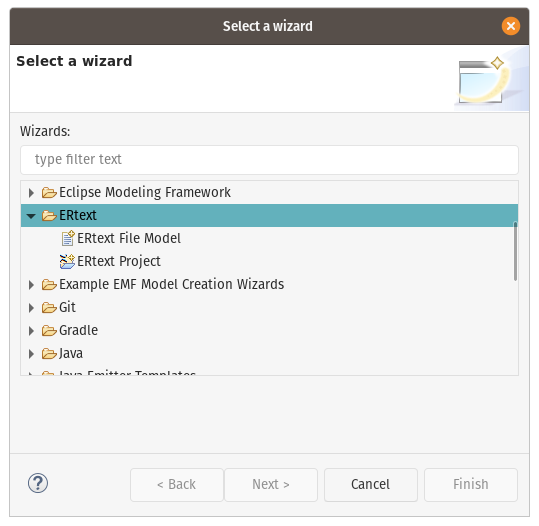
\includegraphics[width=\textwidth]{img/Wizard1.png}
    \fonte{Author.}
  \end{minipage}
  \hfill
  \begin{minipage}[b]{0.55\textwidth}
    \caption{Template proposals.}
    \label{fig:templateProposal}
    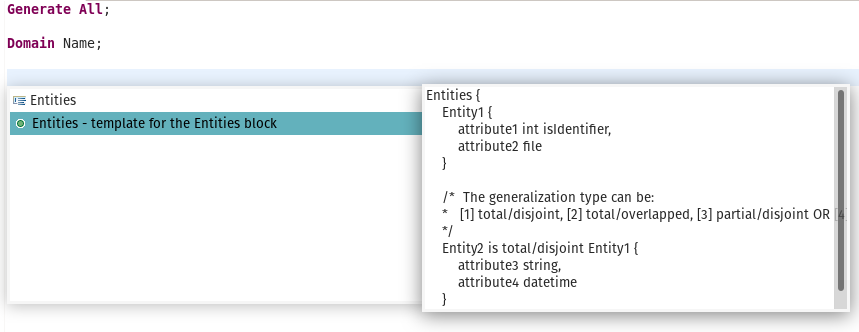
\includegraphics[width=\textwidth]{img/CodeSnippetRecomendation.png}
    \fonte{Author.}
  \end{minipage}
\end{figure}

%------------------------------------------------------------------------------
\subsection{Toy Example}
%------------------------------------------------------------------------------

% Para demonstrar um exemplo de uso vamos imaginar um modelo hipótico de uma rede social simples.
% Neste exemplo existem sete (7) entidades.
% Uma entidade Usuário, que é especializada em Pessoas e Organizações.
% Os Usuários podem compartilhar Postagens, que por sua vez podem conter Fotos associadas.
% Os usuários podem ter relacionamentos de amizade com outros usuários, bem como participar de Grupos.
% Finalmente, para cada relação de Usuários que pertencem a Grupos, nós modelamos um Papel (e.g. dono, moderador, participante, etc).
% Como a relação de Usuários pertencendo a Grupos é uma relação N:N, a adição do Papel gera uma relação ternária (associativa) entra a entidade derivada e as ocorrências de papéis.
% A descrição é exibida na Figura \ref{fig:toyExampleDSlDescription}.

To demonstrate a toy example, let's imagine a hypothetical model of a simple \texttt{social network}.
In this example, there are seven (7) entities.
A \texttt{User} entity, which specializes in the \texttt{People} and \texttt{Organization} entities.
Users can share \texttt{Posts} that may contain associated \texttt{Photos}.
Users can have friendly relationships with other users as well as participate in \texttt{Groups}.
Finally, for each relationship of Users that belong to Groups, we model \texttt{Roles} (\textit{e.g.} owner, moderator, participant, etc) entity.
As the relationship of Users belonging to Groups is an N:N relationship, the addition of Role generates a ternary (associative) relationship between the derived entity and role occurrences.
Figure \ref{fig:toyExampleDSlDescription} shows the description.

\begin{figure}[!htb]
    \centering
    \caption{Description of a social network example.}
    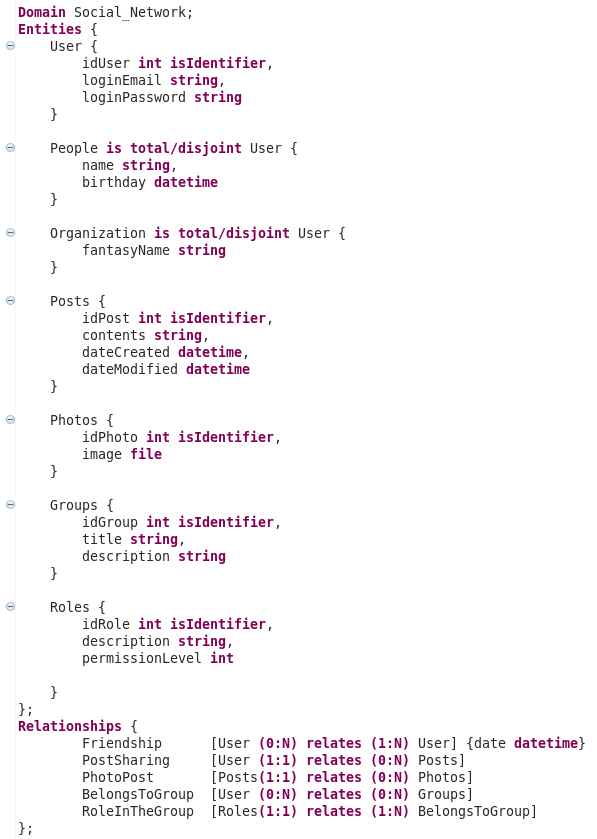
\includegraphics[width=0.5\textwidth]{img/toyExampleDSlDescription.png}
    \fonte{Author.}
    \label{fig:toyExampleDSlDescription}
\end{figure}

% Como dito anteriormente, os geradores são chamados cada vez que o modelo é salvo.
% Se o modelo for considerados válido conforme a sintaxe da \ac{dsl}, o modelo Ecore em memória é despachado para o gerador principal, que então faz um novo encaminhamento para os outros geradores especializados, gerando assim o diagrama, o modelo HTML e os arquivos SQLs.
% Nestes geradores os arquivos destino são gerados em uma pasta chamada src-gen na raiz do projeto.
As stated earlier, the tool calls the generators each time that saves the model.
% As stated earlier, the generators are called each time the model is saved.
If the tool considers the model valid according to the \ac{dsl} syntax, it dispatches the in-memory Ecore model to the main generator. Then forwards it to the other specialized generators, thus producing the diagram (conceptual model), \ac{html} (logical model), and the \ac{sql} files (physical model).
% If the model is considered valid according to the \ac{dsl} syntax, the in-memory Ecore model is dispatched to the main generator, which then forwards it to the other specialized generators, thus producing the diagram (conceptual model), \ac{html} (logical model) and the \ac{sql} files (physical model).
In these generators, the tool generates the target files in a folder called ``src-gen'' at the root of the project folder.

% A representação da herança entre a entidade User e as entidades People e Organization é apresentado na Figura \ref{fig:Diagram_Generalization}. 
% Ao utilizar a PlantUML a notação UML para diagramas de classe é usada.
% O equivalente gerado no modelo lógico é apresentado na Figura \ref{fig:Logical_Generalization}.
Figure \ref{fig:Diagram_Generalization} presents the representation of the inheritance between the \texttt{User} entity and the \texttt{People} and \texttt{Organization} entities.
The tool uses the UML notation for class diagrams when using PlantUML.
Figure \ref{fig:Logical_Generalization} shows the equivalent generated in the logical model.
% The representation of the inheritance among the \texttt{User} entity, the \texttt{People}, and \texttt{Organization} entities is presented in Figure \ref{fig:Diagram_Generalization}.
% When using PlantUML the UML notation for class diagrams is used.
% The equivalent generated in the logical model is shown in Figure \ref{fig:Logical_Generalization}.

\begin{figure}[!htb]
  \centering
  \begin{minipage}[b]{0.4\textwidth}
    \caption{Diagram snippet of a generalization.}
    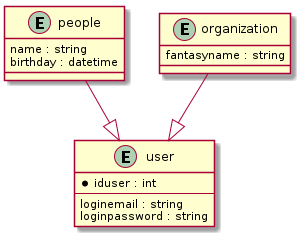
\includegraphics[width=\textwidth]{img/Diagram_Generalization.png}
    \label{fig:Diagram_Generalization}
    \fonte{Author.}
  \end{minipage}
  \hfill
  \begin{minipage}[b]{0.5\textwidth}
    \caption{Logical model snippet of a generalization.}
    \label{fig:Logical_Generalization}
    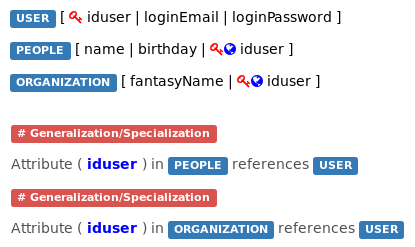
\includegraphics[width=\textwidth]{img/Logical_Generalization.png}
    \fonte{Author.}
  \end{minipage}
\end{figure}

% O modelo SQL gerado, para a plataforma PostgreSQL, também equivalente aos modelos anteriores é apresentado na Figura \ref{fig:SQL_Generalization}
Figure \ref{fig:SQL_Generalization} shows the generated SQL model for the PostgreSQL platform, also equivalent to the previous models.
% The generated SQL model, for the PostgreSQL platform, also equivalent to the previous models, is shown in Figure \ref{fig:SQL_Generalization}

\begin{figure}[!htb]
    \centering
    \caption{SQL model snippet for generalizations.}
    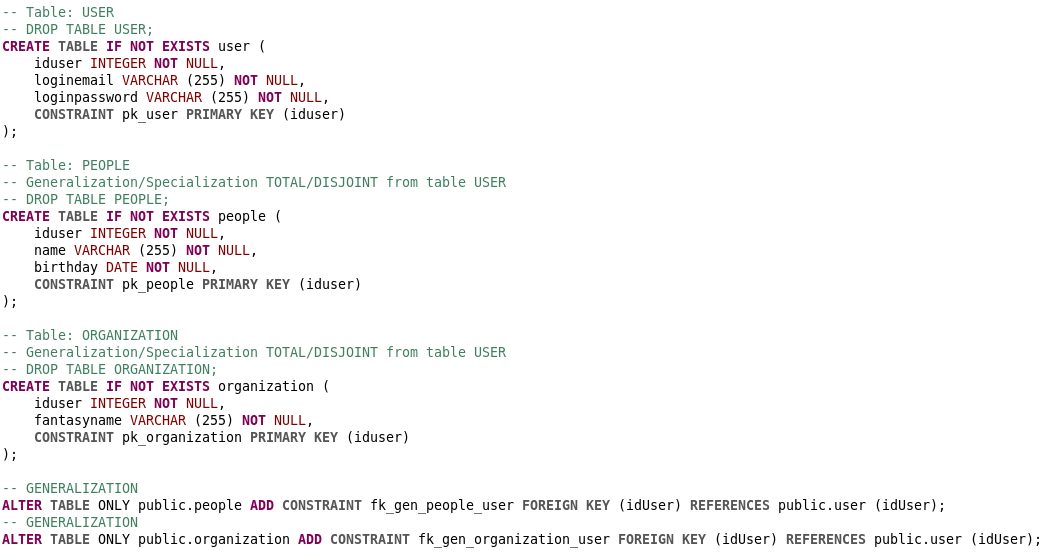
\includegraphics[width=0.9\textwidth]{img/SQL_Generalization.png}
    \fonte{Author.}
    \label{fig:SQL_Generalization}
\end{figure}

% A mesma lógica é usada para relações binárias e entidades tenárias nos modelos lógicos e físicos, ou seja, as entidades são criadas com as referências sendo resolvidas (chaves estrangeiras).
% As relações tem seus mapeamentos sendo indicados logo em seguida da estrutura das entidades.
% Nas Figuras a seguir (\ref{fig:Diagram_Binary} e \ref{fig:Logical_Binary}) os modelos são apresentados com três (3) relações binárias (PostSharing, PhotoPost e FriendShip).
% No modelo conceitual a autorelação N:N Friendship da entidade User é apresentada omitindo a entidade que é derivada.
% Entretanto, no modelo lógico ela é mostrada juntamente com as outras relações, tanto em estrutura quanto nos mapeamentos detectados.
% Para conhecimento, no modelo lógico os simbolos de chave em vermelho representam as chaves primárias.
% Os símbolos de globo em azul representam as chaves estrangeiras.
% Quando um atributo é ambos os tipos de chaves, ambos os símbolos são utilizados.
% A Figura \ref{fig:SQL_Binary} apresenta o modelo \ac{sql} equivalente gerado pela ferramenta.

The same logic is used for binary relationships and ternary entities in both logical and physical models, that is, entities are created with the references being resolved (foreign keys).
The relationships have their mappings being indicated right after the structure of the entities.
In Figures \ref{fig:Diagram_Binary} and \ref{fig:Logical_Binary}, the models are presented with three (3) binary relations (PostSharing, PhotoPost, and FriendShip).
In the conceptual model the N:N Friendship self-relation of the User entity is presented omitting the entity that is derived.
However, in the logical model, it is shown together with the other relationships, both in structure and in the detected mapping list.
For knowledge, the red key symbols represent the primary keys in the logic model.
Blue globe symbols represent foreign keys.
When an attribute is both key types, both symbols are used.
Figure \ref{fig:SQL_Binary} shows the equivalent \ac{sql} model generated by the tool.

\begin{figure}[!htb]
  \centering
  \begin{minipage}[b]{0.4\textwidth}
    \caption{Diagram snippet with binary relatioships.}
    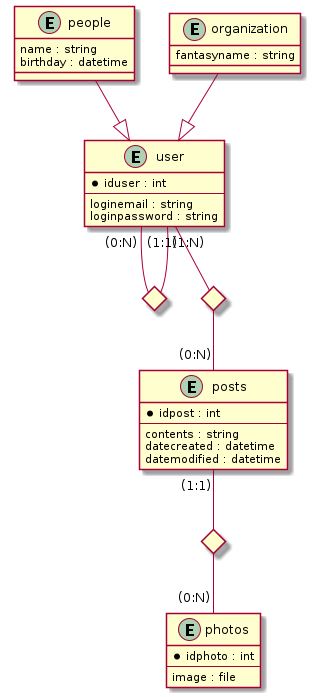
\includegraphics[width=0.8\textwidth]{img/Diagram_binary.png}
    \label{fig:Diagram_Binary}
    \fonte{Author.}
  \end{minipage}
  \hfill
  \begin{minipage}[b]{0.5\textwidth}
    \caption{Logical model snippet with binary relatioships.}
    \label{fig:Logical_Binary}
    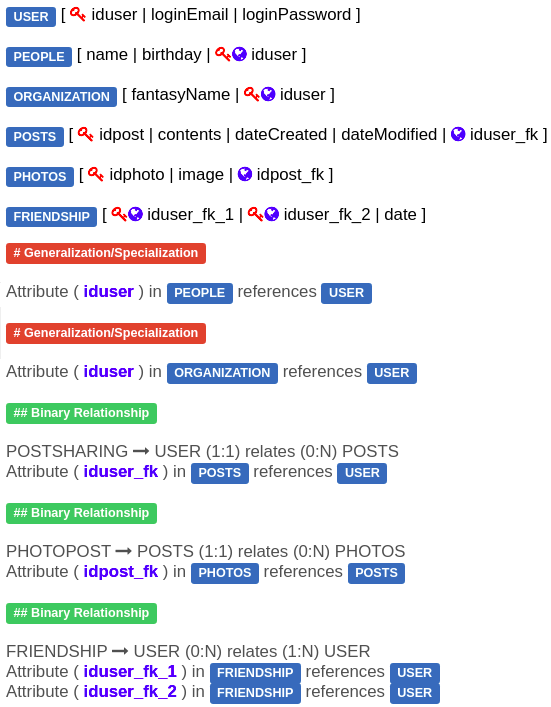
\includegraphics[width=0.8\textwidth]{img/Logical_binary.png}
    \fonte{Author.}
  \end{minipage}
\end{figure}

\begin{figure}[!htb]
    \centering
    \caption{SQL model snippet with binary relationships.}
    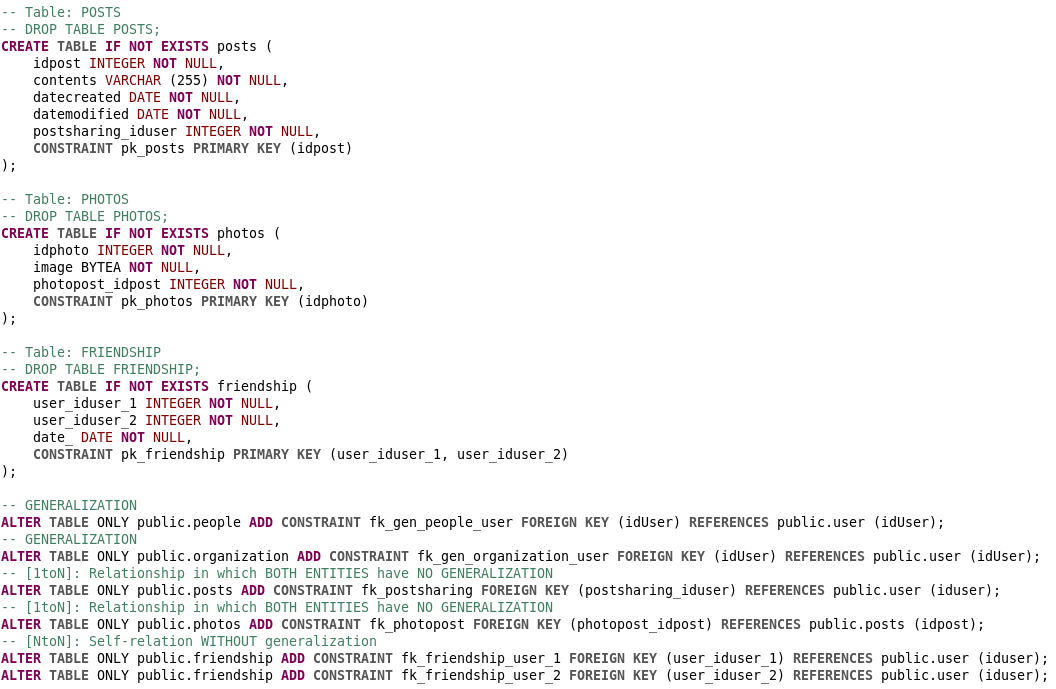
\includegraphics[width=0.8\textwidth]{img/SQL_Binary.png}
    \fonte{Author.}
    \label{fig:SQL_Binary}
\end{figure}

% No que diz respeito as relações ternárias (associativas) quando um diagrama é gerado há a indição onde elas ocorrem na imagem com a ajuda de uma anotação.
% No modelo lógico é exibida a entidade derivada deste tipo de relação.
% Basicamente, há a associação entre uma relação N:N com outra entidade.
% Para melhor compreensão do usuário, nós mantemos o mesmo padrão de apresentação, fazendo uso de rótulos coloridos indicando o tipo de mapeamento detectado.
% As Figuras \ref{fig:Diagram_Ternary} e \ref{fig:Logical_Ternary} mostram um fragmento deste tipo específico de relação sendo mapeada na nossa ferramenta, com base no modelo descrito no ínicio desta seção.
Concerning ternary (associative) relationships, when it generates a diagram, there is an indication of where they occur in the image with the help of an annotation.
% With respect to ternary (associative) relationships, when a diagram is generated there is an indication of where they occur in the image with the help of an annotation.
In the logical model, the entity derived from this type of relationship is displayed.
Basically, there is an association between an N:N relationship with another entity.
% For better user understanding, we keep the same presentation pattern, making use of colored labels indicating the type of mapping detected.
For better user understanding, we keep the same presentation pattern using colored labels that indicate the mapping detected type.
% Figures \ref{fig:Diagram_Ternary} and \ref{fig:Logical_Ternary} show a fragment of this specific type of relationship being mapped in our tool, based on the model described at the beginning of this section.
Figures \ref{fig:Diagram_Ternary} and \ref{fig:Logical_Ternary} show a fragment of this specific relationship type mapped in our tool based on the model described at the beginning of this section.

\begin{figure}[!htb]
  \centering
  \begin{minipage}[b]{0.4\textwidth}
    \caption{Diagram snippet with a ternary relationship.}
    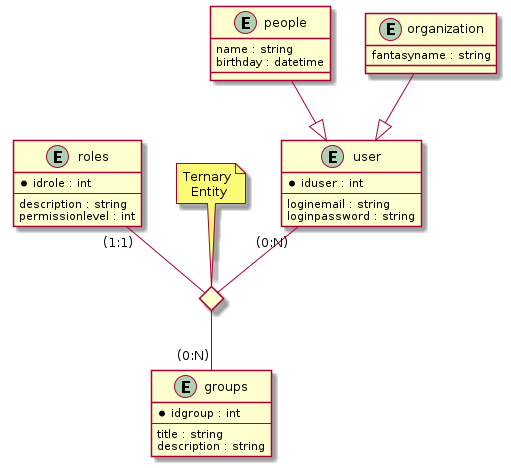
\includegraphics[width=\textwidth]{img/Diagram_Ternary.png}
    \label{fig:Diagram_Ternary}
    \fonte{Author.}
  \end{minipage}
  \hfill
  \begin{minipage}[b]{0.5\textwidth}
    \caption{Logical model snippet with a ternary relationship.}
    \label{fig:Logical_Ternary}
    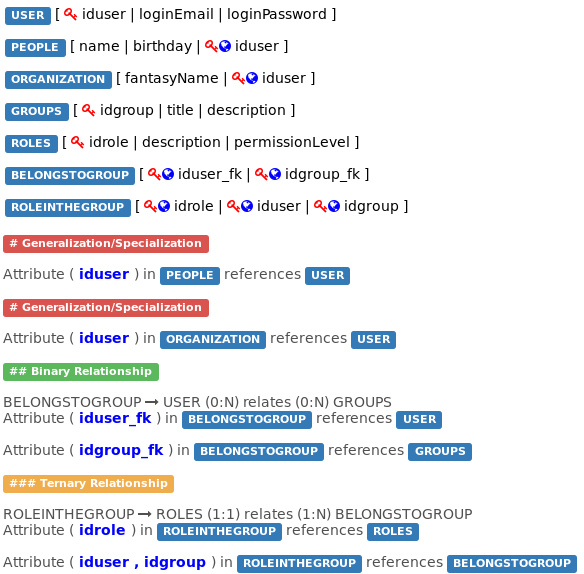
\includegraphics[width=0.8\textwidth]{img/Logical_Ternary.png}
    \fonte{Author.}
  \end{minipage}
\end{figure}

\begin{figure}[!htb]
    \centering
    \caption{SQL model snippet with a ternary relationship.}
    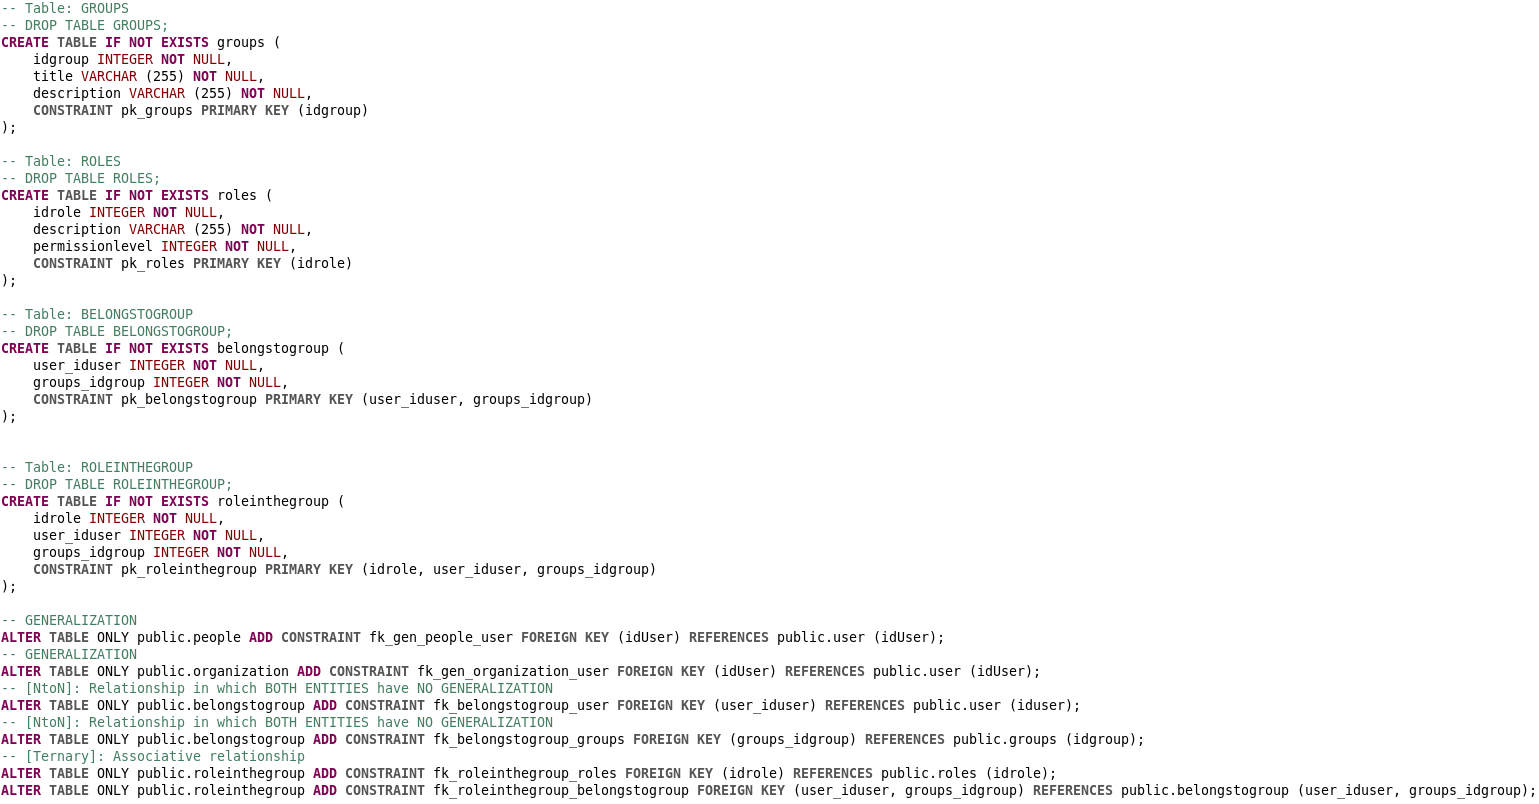
\includegraphics[width=\textwidth]{img/SQL_Ternary.png}
    \fonte{Author.}
    \label{fig:SQL_Ternary}
\end{figure}


% Finalmente, o mapeamento para o arquivo \ac{sql} apresentado na Figura \ref{fig:SQL_Ternary} segue também o mesmo padrão, gerando os comandos \texttt{Alter Table} após a definição da estrutura das entidades.
% Algo que é importante de se relatar é que inicialmente os modelos \ac{sql} estavam sendo criados com as restriçoes chaves estrangeiras sendo declaradas já no corpo das tabelas.
% Isso foi feito por acreditarmos que a legibilidade e compreensão das \ac{ddl} era facilitada.
% Contudo, foi necessário um reavaliação desta estratégia uma vez que os códigos \ac{sql} gerados não estavam sendo executados nas plataformas alvo.
% Isso acontecia pois se tornou díficil prever quando uma restrição indicava relação com algum atributo de entidade ainda não criada.
% Tentou-se implementar formas de se fazer a geração da ordem correta mas por conta da complexidade que se apresentou aderimos a criação das restrições via comandos \texttt{Alter Table} no final do arquivo, assim os tornando executáveis nos \ac{rdms}.
Finally, Figure \ref{fig:SQL_Ternary} shows the mapping to the \ac{sql} file also follows the same pattern, generating the \texttt{Alter Table} commands after defining the structure of the entities.
Something relevant to report is that firstly the \ac{sql} models were being created with the foreign key constraints being declared already in the bodies of the tables.
It was done because we believed that facilitates the readability and the understanding of \ac{ddl}.
% This was done because we believed that the readability and understanding of \ac{ddl} were facilitated.
However, it was necessary to re-evaluate this strategy since the generated \ac{sql} codes were not being executed successfully on the target platforms.
This happened because it became difficult to predict when a restriction indicated a relationship with some attribute of an entity not yet created.
We tried to implement ways to generate the correct order, despite due to the complexity that presented itself, we adhered to the creation of restrictions via \texttt{Alter Table} commands at the end of the file, thus making them executable in the \acp{dbms}.
% We tried to implement ways to generate the correct order, but due to the complexity that presented itself, we adhered to the creation of restrictions via \texttt{Alter Table} commands at the end of the file, thus making them executable in the \acp{dbms}.

%------------------------------------------------------------------------------
\section{Chapter Lessons}
%------------------------------------------------------------------------------
 
% Neste capítulo foram expostos os requisitos, as decisões de projeto e a arquitetura da \ac{dsl} proposta para a solução desenvolvida. 
% Também é apresentada uma visão geral da versão estável que será testada na última avaliação experimental, bem como um exemplo de uso foi descrito, com os respectivos artefatos produzidos pelos geradores sendo exibidos.
In this chapter, we have laid out the requirements, design decisions, and architecture for the developed solution.
We also have presented an overview of the stable version that will test in the next experimental evaluation. 
Furthermore, we described an example of use with the respective artifacts produced by the generators.
% In this chapter, the requirements, design decisions and architecture of the \ac{dsl} proposal for the developed solution were exposed.
% An overview of the stable version that will be tested in the last experimental evaluation is also presented, as well as an example of use was described, with the respective artifacts produced by the generators being displayed.

% Novamente reforçamos a importância da comunidade Xtext formada por um grupo de desenvolvedores que ajudaram direta e indiretamente na implementação de grande parte da ferramenta apresentada.
% Através das interações com estes desenvolvedores houve um amadurecimento da nossa proposta, bem como nós adquirimos uma gama de habilidades técnicas e pessoais (habilidades soft e hard) que auxiliaram decisivamente no processo de otimização da DSL e do código de infraestrutura fornecida pelo framework.
Again, we reinforce the importance of the Xtext community formed by a group of developers who helped, directly and indirectly, the implementation of a large part of the presented tool.
Through interactions with these developers, our proposal matured,  even as we acquired a range of technical and personal skills (soft and hard skills) that decisively helped in the optimization process of the \ac{dsl} and the infrastructure code provided by the framework.

% Esperamos que a ferramenta de modelagem desenvolvida possa colaborar com o processo de ensino-aprendizagem, fornecendo uma gramática de fácil compreensão e uma facilidade de uso facilitado pela integração com a IDE Eclipse. 
% Finalmente, para que este objetivo seja alcançado, é imprescindível que a avaliação experimental seja devidamente planeada, executada e analisada tendo em conta as funcionalidades que nos propomos oferecer.
We hope that the developed modeling tool can collaborate with the teaching-learning process, providing an easy-to-understand grammar and ease of use facilitated by the Eclipse \ac{ide} integration.
% We hope that the developed modeling tool can collaborate with the teaching-learning process, providing an easy-to-understand grammar and ease of use facilitated by the integration with the Eclipse \ac{ide}.
Finally, to achieve this goal, the experimental evaluation must be duly planned, executed, and analyzed, taking into account the features that we propose to offer.
% Finally, in order to achieve this goal, it is imperative that the experimental evaluation be properly planned, executed, and analyzed taking into account the features that we propose to offer.



%==============================================================================
\chapter{Experimental Evaluations}\label{chap:experiments}
% Avaliação preliminar para a qualificação
%==============================================================================

In this chapter, we present the research questions and hypotheses investigated during the evaluation of our proposal. 
In addition, we present the experimental design adopted and its conduction.
Section \ref{sec_experiments:preliminaryEval} presents the first evaluation of ERText, which focuses on the tool features assessment.
Section \ref{sec_experiments:finalEval} describes the execution of two other experiments carried out in December 2021 and February 2022, which also included the evaluation of artifacts generated by the tools and learning aspects.
In the end, Section \ref{sec_experiments:lessons} draws the chapter's lessons.

%------------------------------------------------------------------------------
\section{Tool Features - Experiment 1} 
\label{sec_experiments:preliminaryEval}
%------------------------------------------------------------------------------

This section presents all the planning, conduction, the results obtained discussion, threats to validity of the study, and the conclusions regarding the preliminary evaluation carried out to evaluate the first release of a stable prototype of the developed tool.

%######################################################
\subsection{Planning}
\label{ssec_experiments:preliminary_planning}
%######################################################

We carried out this preliminary evaluation from the replication of the experimental protocol performed in a previous study~\cite{Lopes:2019}, which aimed to obtain evidence of the comparison from two approaches for modeling relational databases, one graphical and the other textual.
% This preliminary evaluation was carried out from the replication of the experimental protocol performed in a previous study~\cite{Lopes:2019} and aims to obtain evidence from the comparison of two approaches for modeling relational databases, one graphical and the other textual.

We specified the following treatments:
\begin{enumerate} [label=\roman*.]
    \item Control treatment: the brModelo tool (graphical approach) and;
    \item Experimental treatment: the ERtext tool (textual approach).
\end{enumerate}
This replication goal is to evaluate the feasibility of using a textual approach to support the teaching-learning process of conceptual modeling relational databases.
% The purpose of this replication is to evaluate the feasibility of using a textual approach to support the teaching-learning process of conceptual modeling relational databases.

\textbf{Context:}
% The context of the experiment is characterized according to four dimensions:
We characterized the context of the experiment according to four dimensions:
\begin{enumerate}[label=\roman*.]
    \item Process: Process: it used an \textit{in-vitro} approach since we performed the tasks under controlled conditions;
    % Process: an \textit{in-vitro} approach was used, since the tasks were performed under controlled conditions.
    %In software engineering, most \textit{in-vitro} experiments are executed in universities or among selected groups of a software development organization~\cite{Travassos:2003}.
    \item Subjects: undergrad students in Computer Science (CS) and Software Engineering (SE) programs;
    \item. Reality: the experiment addressed a real problem, \textit{i.e.}, the difference in the effort spent by subjects in the conceptual modeling of relational databases; 
    %the artifacts quality produced and the subjects Perceived Usefulness (PU) using both approaches.
    \item Generality: we inserted this evaluation in a specific context involving database modeling students.
    However, we can replicate the general ideas of this experiment in another set of subjects, approaches, or DSLs that support database designing. 
    % However, the general ideas of this experiment can be replicated in another set of subjects, approaches or DSLs that support database designing.
\end{enumerate}

\textbf{Research Questions (RQs):}
Regards the discussion of controlled experiment results, we decided to formulate four RQs related to the activities performed in the protocol execution.
% For the controlled experiment results discussion, we decided to formulate four RQs related to the activities performed in the execution of the protocol.
\begin{itemize}
    \item \textbf{RQ1.} Which approach requires the most effort spent on average during the modeling activity?
    \item \textbf{RQ2.} What is the quality level of the models produced using the graphical and textual approaches?
    \item \textbf{RQ3.} What is the subject's perception regarding the Perceived Ease of Use (PEoU) and Perceived Usefulness (PU) of the proposed DSL?
    \item \textbf{RQ4.} What is the subject's assessment concerning the representation of the ER modeling builders supported in the proposed DSL?
\end{itemize}

\textbf{Hypotheses Formulation:} 
% The first two RQs were taken into account. 
We have taken into account the first two RQs. 
Regarding \textbf{RQ1.} the average effort spent required using each approach, our scientific hypotheses are as follows:
% we defined a two-sided hypotheses that measure the average effort spent between textual and graphical approaches during conceptual modeling. State the null (no difference) $H_0 : \mu Time_T = \mu Time_G$ and alternative (significant difference) $H_a : \mu Time_T \neq Time_G$ hypotheses.
\begin{itemize}
    \item \textbf{Null hypothesis:} $H_0 : \mu Time_T = \mu Time_G$: There is no difference in the measure of average effort spent between textual and graphical approaches during conceptual modeling.
    \item \textbf{Alternative hypothesis:} $H_{1} : \mu Time_T \neq \mu Time_G$: There is a significant difference in the measure of average effort spent between textual and graphical approaches during conceptual modeling.
\end{itemize}
Regarding \textbf{RQ2.} 
%the modeling effectiveness using each approach, our hypotheses are as follows:
in the same way, we stated two-sided hypotheses that measure the modeling effectiveness between textual and graphical approaches during conceptual modeling.
% The null (no difference) and alternative (significant difference) hypotheses are, respectively: 
% $H_0 : \mu Effectiveness_T = \mu Effectiveness_G$ and 
% $H_a : \mu Effectiveness_T \neq \mu Effectiveness_G$.
\begin{itemize}
    \item \textbf{Null hypothesis:} $H_0 : \mu Effectiveness_T = \mu Effectiveness_G$: There is no difference in effectiveness measures between textual and graphical approaches during conceptual modeling.
    \item \textbf{Alternative hypothesis:} $H_{1} : \mu Effectiveness_T \neq \mu Effectiveness_G$: There is a significant difference in effectiveness measures between textual and graphical approaches during conceptual modeling.
\end{itemize}

\textbf{Statistical Methods:} Unlike the first experiment, this replication included a change in the statistical methods adopted.
Previously, we have used the Shapiro-Wilk normality test and the paired T-test for dependent samples.
Hence, this happened because the sample was smaller (27) than 30 elements.
% This was because the sample was smaller (27) than 30 elements.
However, the literature recommends alternative tests for samples equal to or greater than this quantity~\cite{Triola:2018}.
% However, for samples equal to or greater than this quantity, alternative tests are recommended~\cite{Triola:2018}.

For the effort, we chose the Kolmogorov-Smirnov test to verify normality and the Wilcoxon Signed-Rank test for paired samples to investigate the hypotheses using the time spent metric.
In short, the Kolmogorov-Smirnov two-sample test is used to test the agreement between two cumulative distributions.
The null hypothesis in this method states that there is no difference between the two distributions.
A simplified version of the method is given in the Equation \ref{eq:KS}:

\begin{equation}
\label{eq:KS}
    %\[ 
    D = Max|F_{n1}(X) - F_{n2}(X)|
    %\]
\end{equation}

Where \textit{n1} and \textit{n2} are the values observed in the distributions, respectively, and the \textbf{\textit{D}} represents the large maximum deviation indicating towards a difference between the two sample distributions. 

Furthermore, the Wilcoxon Signed-Rank test for dependent samples compares a sample median against a hypothetical median.
Initially, the hypothetical mean, $\mu_0$ , is subtracted from each data value. 
Then, we classified the values according to their absolute values.
% Then, the values are classified according to their absolute values.
Next, we calculated the sum of the positive ranks $Sp$ and the sum of the negative ranks $Sn$. 
In the statistical test, $W_R$ is the minimum of $Sp$ and $Sn$. 
With this, it is possible to calculate the mean and standard deviation of $W_R$ using the simplified version of the formulas shown below in Equations \ref{eq:WSR1} and \ref{eq:WSR2}, where $t$ represents the number of times the $i^th$ value occurs.
Then, we finally calculated the \textit{z-value} using Equation \ref{eq:WSR3}.
% Then, the \textit{z-value} is finally calculated using the Equation \ref{eq:WSR3}.

\begin{equation}
\label{eq:WSR1}
   ^\mu W_R~=~\frac{n(n+1)}{4}
\end{equation}

\begin{equation}
\label{eq:WSR2}
    ^\sigma W_R~=~\frac{n(n+1)(2n+1)}{24}-\frac{\Sigma~t^3~-~\Sigma~t}{48}
\end{equation}

\begin{equation}
\label{eq:WSR3}
    Z_W~=~\frac{W_R~-~^\mu W_R}{^\sigma W_R}
\end{equation}

For the effectiveness tests, we have adopted the same statistical methods despite instead of using the time spent metric, another measure was necessary.
Thus, we have performed the F1 calculations, deriving from the harmonic mean of precision and recall metrics, for each model produced in both approaches.
% Thus, we have performed the F1 calculations, which is derived from the harmonic mean of \textit{Precision} and \textit{Recall} metrics, for each of the models produced in both approaches.
The F1 calculation~\cite{Derczynski:2016} takes into account variables known as \textit{True Positives}, \textit{False Positives}, and \textit{False Negatives}.
\begin{description}
% \begin{inparadesc}
    \item \textbf{\textit{True Positives (TP)}}: Number of elements correctly modeled using the approach.
    \item \textbf{\textit{False Positives (FP)}}: Number of elements incorrectly modeled using the approach. 
    \item \textbf{\textit{False Negatives (FN)}}: Number of elements not modeled using the approach.
% \end{inparadesc}
\end{description}
From the identification of the variables, it is then possible to calculate the \textit{Precision}, \textit{Recall}, and \textit{F1} of each model according to these formulas:
% From the variables identification it is then possible to calculate the \textit{Precision}, \textit{Recall}, and \textit{F1} of each model according to these formulas:
\begin{description}
    \item \textbf{\textit{Precision (PR)}}: $\frac{TP}{TP~+~FP}$ 
    \hfill 
    \textbf{\textit{Recall (RE)}}:$\frac{TP}{TP~+~FN}$
    \hfill
    \textbf{\textit{F1-Score (F1)}}: $\frac{2~*~(PR~*~ RE)}{PR~+~RE}$
\end{description}

\textbf{Experiment Design:} Finally, Figure \ref{fig:designExp} presents the design of the controlled experiment performed. 
We followed the design of one factor with two treatments, where we blocked, balanced, and randomized the subjects, which carried out both treatments, featuring a paired comparison design.

\begin{figure}[!htb]
    \centering
    \caption{Experiment design.}
    \label{fig:designExp}
    

\tikzset{every picture/.style={line width=0.75pt}} %set default line width to 0.75pt        

\begin{tikzpicture}[x=0.9pt,y=0.9pt,yscale=-1,xscale=1]
%uncomment if require: \path (0,327); %set diagram left start at 0, and has height of 327


%Shape: Ellipse [id:dp633810982278807] 
\draw  [line width=1.5]  (84.73,72.26) .. controls (84.73,55.52) and (102.16,41.96) .. (123.66,41.96) .. controls (145.16,41.96) and (162.59,55.52) .. (162.59,72.26) .. controls (162.59,88.99) and (145.16,102.56) .. (123.66,102.56) .. controls (102.16,102.56) and (84.73,88.99) .. (84.73,72.26) -- cycle ;



%Shape: Ellipse [id:dp7904221795411808] 
\draw  [line width=1.5]  (378.89,75.63) .. controls (378.89,62.05) and (394.88,51.04) .. (414.61,51.04) .. controls (434.33,51.04) and (450.32,62.05) .. (450.32,75.63) .. controls (450.32,89.21) and (434.33,100.22) .. (414.61,100.22) .. controls (394.88,100.22) and (378.89,89.21) .. (378.89,75.63) -- cycle ;

%Rounded Rect [id:dp5302697683495847] 
\draw  [line width=1.5]  (180.95,87.75) .. controls (180.95,85.09) and (183.11,82.93) .. (185.77,82.93) -- (200.23,82.93) .. controls (202.9,82.93) and (205.06,85.09) .. (205.06,87.75) -- (205.06,140.25) .. controls (205.06,142.91) and (202.9,145.07) .. (200.23,145.07) -- (185.77,145.07) .. controls (183.11,145.07) and (180.95,142.91) .. (180.95,140.25) -- cycle ;
%Rounded Rect [id:dp9616486966995694] 
\draw  [line width=1.5]  (180.95,14.03) .. controls (180.95,11.37) and (183.11,9.21) .. (185.77,9.21) -- (200.23,9.21) .. controls (202.9,9.21) and (205.06,11.37) .. (205.06,14.03) -- (205.06,66.52) .. controls (205.06,69.19) and (202.9,71.35) .. (200.23,71.35) -- (185.77,71.35) .. controls (183.11,71.35) and (180.95,69.19) .. (180.95,66.52) -- cycle ;

%Shape: Rectangle [id:dp03801896284105699] 
\draw  [line width=1.5]  (222.23,24.87) -- (277.28,24.87) -- (277.28,58.21) -- (222.23,58.21) -- cycle ;
%Straight Lines [id:da1799424135415575] 
\draw    (163.93,73.09) -- (177.61,61.43) ;
\draw [shift={(179.89,59.48)}, rotate = 499.54] [fill={rgb, 255:red, 0; green, 0; blue, 0 }  ][line width=0.08]  [draw opacity=0] (8.93,-4.29) -- (0,0) -- (8.93,4.29) -- cycle    ;
%Straight Lines [id:da17029537209985257] 
\draw    (163.93,73.09) -- (177.81,87.53) ;
\draw [shift={(179.89,89.69)}, rotate = 226.13] [fill={rgb, 255:red, 0; green, 0; blue, 0 }  ][line width=0.08]  [draw opacity=0] (8.93,-4.29) -- (0,0) -- (8.93,4.29) -- cycle    ;
%Straight Lines [id:da39402523544663426] 
\draw  [dash pattern={on 4.5pt off 4.5pt}]  (277.5,92.15) -- (307.06,61.21) ;
\draw [shift={(309.13,59.04)}, rotate = 493.69] [fill={rgb, 255:red, 0; green, 0; blue, 0 }  ][line width=0.08]  [draw opacity=0] (8.93,-4.29) -- (0,0) -- (8.93,4.29) -- cycle    ;
%Straight Lines [id:da7992081880522388] 
\draw  [dash pattern={on 4.5pt off 4.5pt}]  (277.28,58.21) -- (307.27,89.16) ;
\draw [shift={(309.35,91.31)}, rotate = 225.9] [fill={rgb, 255:red, 0; green, 0; blue, 0 }  ][line width=0.08]  [draw opacity=0] (8.93,-4.29) -- (0,0) -- (8.93,4.29) -- cycle    ;
%Right Arrow [id:dp3913444800583221] 
\draw  [line width=1.5]  (11.57,42.74) -- (55.14,42.74) -- (55.14,31.99) -- (82.78,73.11) -- (55.14,114.23) -- (55.14,103.49) -- (11.57,103.49) -- cycle ;
%Shape: Rectangle [id:dp003852149638719382] 
\draw  [line width=1.5]  (310.31,24.87) -- (365.36,24.87) -- (365.36,58.21) -- (310.31,58.21) -- cycle ;
%Shape: Rectangle [id:dp0126542660109914] 
\draw  [line width=1.5]  (310.31,92.18) -- (365.36,92.18) -- (365.36,125.52) -- (310.31,125.52) -- cycle ;
%Shape: Rectangle [id:dp4954877903085966] 
\draw  [line width=1.5]  (222.23,92.18) -- (277.28,92.18) -- (277.28,125.52) -- (222.23,125.52) -- cycle ;
%Straight Lines [id:da3442884963113835] 
\draw    (365.36,58.21) -- (377.4,64.63) ;
\draw [shift={(380.04,66.05)}, rotate = 208.07999999999998] [fill={rgb, 255:red, 0; green, 0; blue, 0 }  ][line width=0.08]  [draw opacity=0] (8.93,-4.29) -- (0,0) -- (8.93,4.29) -- cycle    ;
%Straight Lines [id:da6883068419855551] 
\draw    (365.36,92.18) -- (377.84,86.46) ;
\draw [shift={(380.57,85.22)}, rotate = 515.4100000000001] [fill={rgb, 255:red, 0; green, 0; blue, 0 }  ][line width=0.08]  [draw opacity=0] (8.93,-4.29) -- (0,0) -- (8.93,4.29) -- cycle    ;
%Rounded Rect [id:dp5928061300931144] 
\draw  [line width=1.5]  (478.27,37.32) .. controls (478.27,34.68) and (480.41,32.55) .. (483.04,32.55) -- (497.34,32.55) .. controls (499.97,32.55) and (502.1,34.68) .. (502.1,37.32) -- (502.1,112.96) .. controls (502.1,115.59) and (499.97,117.72) .. (497.34,117.72) -- (483.04,117.72) .. controls (480.41,117.72) and (478.27,115.59) .. (478.27,112.96) -- cycle ;

%Straight Lines [id:da6932528701926595] 
\draw    (450.32,75.46) -- (472.85,75.45) ;
\draw [shift={(475.85,75.45)}, rotate = 539.96] [fill={rgb, 255:red, 0; green, 0; blue, 0 }  ][line width=0.08]  [draw opacity=0] (8.93,-4.29) -- (0,0) -- (8.93,4.29) -- cycle    ;
%Straight Lines [id:da7950818392289087] 
\draw    (40.46,131.56) -- (40.46,109.39) ;
\draw [shift={(40.46,107.39)}, rotate = 450] [color={rgb, 255:red, 0; green, 0; blue, 0 }  ][line width=0.75]    (10.93,-4.9) .. controls (6.95,-2.3) and (3.31,-0.67) .. (0,0) .. controls (3.31,0.67) and (6.95,2.3) .. (10.93,4.9)   ;
%Straight Lines [id:da5784112946450906] 
\draw    (414.54,135.73) -- (414.54,107.33) ;
\draw [shift={(414.54,105.33)}, rotate = 450] [color={rgb, 255:red, 0; green, 0; blue, 0 }  ][line width=0.75]    (10.93,-4.9) .. controls (6.95,-2.3) and (3.31,-0.67) .. (0,0) .. controls (3.31,0.67) and (6.95,2.3) .. (10.93,4.9)   ;
%Straight Lines [id:da04489153588175898] 
\draw    (206.5,42.65) -- (218.97,42.92) ;
\draw [shift={(221.97,42.99)}, rotate = 181.23] [fill={rgb, 255:red, 0; green, 0; blue, 0 }  ][line width=0.08]  [draw opacity=0] (8.93,-4.29) -- (0,0) -- (8.93,4.29) -- cycle    ;
%Straight Lines [id:da30869554668079413] 
\draw    (205.97,109.89) -- (218.45,110.16) ;
\draw [shift={(221.44,110.22)}, rotate = 181.23] [fill={rgb, 255:red, 0; green, 0; blue, 0 }  ][line width=0.08]  [draw opacity=0] (8.93,-4.29) -- (0,0) -- (8.93,4.29) -- cycle    ;




% Text Node
\draw (249.75,48.63) node  [font=\scriptsize] [align=left] {Approach};
% Text Node
\draw (249.75,34.46) node  [font=\scriptsize] [align=left] {Graphical};
% Text Node
\draw (490.19,75.14) node  [font=\footnotesize,rotate=-270] [align=left] {Analisys};
% Text Node
\draw (414.31,168.64) node  [font=\footnotesize] [align=left] {Qualitative Evaluation};
% Text Node
\draw (414.31,155.81) node  [font=\footnotesize] [align=left] {and};
% Text Node
\draw (414.31,143.84) node  [font=\footnotesize] [align=left] {Produced Models};
% Text Node
\draw (187.85,136.5) node [anchor=north west][inner sep=0.75pt]  [font=\footnotesize,rotate=-270] [align=left] {Group 2};
% Text Node
\draw (337.84,34.46) node  [font=\scriptsize] [align=left] {Graphical};
% Text Node
\draw (337.84,48.63) node  [font=\scriptsize] [align=left] {Approach};
% Text Node
\draw (249.75,101.76) node  [font=\scriptsize] [align=left] {Textual};
% Text Node
\draw (249.75,115.93) node  [font=\scriptsize] [align=left] {Approach};
% Text Node
\draw (337.84,101.76) node  [font=\scriptsize] [align=left] {Textual};
% Text Node
\draw (337.84,115.93) node  [font=\scriptsize] [align=left] {Approach};
% Text Node
\draw (414.61,66.67) node  [font=\footnotesize] [align=left] {Data};
% Text Node
\draw (414.61,81.26) node  [font=\footnotesize] [align=left] {Gathering};
% Text Node
\draw (40.22,138.89) node  [font=\footnotesize] [align=left] {Background};
% Text Node
\draw (40.22,152.23) node  [font=\footnotesize] [align=left] {Survey};
% Text Node
\draw (123.66,64.96) node  [font=\scriptsize] [align=left] {Balancing};
% Text Node
\draw (123.66,79.56) node  [font=\scriptsize] [align=left] {Randomization};
% Text Node
\draw (186.5,62.78) node [anchor=north west][inner sep=0.75pt]  [font=\footnotesize,rotate=-270] [align=left] {Group 1};
% Text Node
\draw (45.21,73.11) node  [font=\footnotesize] [align=left] {33 Subjects};


\end{tikzpicture}

    % \includegraphics[width=\columnwidth]{images/DesignExperimento.png}
    \fonte{Author.}
\end{figure}

%###########################################################
\subsection{Conduction}
\label{ssec_experiments:preliminary_conduction}
%###########################################################

\textbf{Preparation:} 
Initially, we held remote meetings between the researchers involved to define the planning and the adopted operation mode in response to the current exception scenario due to the worldwide pandemic.
% Initially, remote meetings were held between the researchers involved to define the planning and the mode of operation that should be adopted, in response to the current scenario of exception due to the worldwide pandemic.
As a result, we defined activities adapted from the first experiment conducted in person.
% As a result, activities were defined that should be adapted in relation to the first experiment, which was conducted in person.
Hence, to capture a significant sample for the object of study, we decided to contact the professors responsible for teaching, in the first half of 2021, two courses of different undergraduate courses: Database (SE) and Database I (CS).
% In order to capture a significant sample for the object of study, it was decided to contact the professors responsible for teaching two courses of different undergraduate courses: Database (SE) and Database I (CS) in the first half of 2021.
% With the initial objectives aligned, the collaborating teachers made the disclosure of profile questionnaires (Google Forms) to the subjects.
Once the initial objectives aligned, the collaborating teachers disclosed the profile questionnaires (Google Forms) to the subjects.

We reused the four (4) instruments from the original experiment. 
% The four (4) instruments from the original experiment were reused. 
The first two were modeling problems with similar levels of complexity, while the last two were qualitative assessments.
% The first two were modeling problems with similar levels of complexity, while the last two were of qualitative assessment.
For respecting the health security protocols required (social distancing), we decided to carry out the activities remotely.
% We decided that the activities would carry out remotely, respecting the health security protocols required (social distancing). 
% It was decided that the activities would be carried out remotely, respecting the health security protocols required (social distancing). 
For this purpose, we prepared a virtual machine with the tools installed, even as the instruments and supporting materials. 
% For this purpose, a virtual machine was prepared with the tools installed, as well as the instruments and supporting materials. 
This virtual machine had accessed on the university's computers by the subjects using their institutional credentials.
% This virtual machine should be accessed on the university's computers by the subjects using their institutional credentials.

\textbf{Execution:} 
The profile form also served as a term of participation since the presence in the experiment was voluntary.
With this information, we have randomized the subjects to define the groups.
% With this information, the subjects were then randomized to define the groups.
We did not find wide discrepancies among the subjects' knowledge levels, demonstrating a homogeneous sample in general.
% We found that there were no major discrepancies between the levels of knowledge of the subjects, demonstrating that there was a homogeneous sample in general.
On the experiment day, the first activity that we performed was a brief initial presentation.
% On the experiment day, the first activity carried out was a brief initial presentation.
Then, the training phase for the participants began.
During this phase, we have presented the two database modeling tools used in the experiment, providing an overview of the operation and answering possible questions that arose.
% During this phase, the two database modeling tools that would be used were presented, providing an overview of the operation and answering possible questions that arose.
The training phase included watching videos to demonstrate both tools: brModelo, and our proposal, respectively.

Then, we start the modeling phase of the proposed problems.
All subjects accessed the virtual machines with the problems provided in PDF documents.
% When starting Instrument 1, all participants were informed with which tool they should develop the solution, thus respecting the groups to which they were part.
When starting Instrument 1, we informed which tool each participant should develop the solution, thus respecting the group of which one was part.
We asked the subjects to write down the start and end times of the tasks for each instrument they performed.
We stipulated no time limit for completion according to the subjects who completed the modeling task. 
We asked them to comply with the guidelines included in the support material for saving the generated artifacts.
% We stipulated no time limit for completion and, according to the subjects completed the modeling task, they were asked to comply with the guidelines included in the support material for saving the generated artifacts.
With the models saved, we informed the subjects that they should move on to the next task described in Instrument 2, although it was necessary to use the reverse approach to the one they had initially used.

Since the subjects concluded the instruments of the data modeling problems, we delivered the qualitative assessment instruments.
% At the end of the instruments that contained the modeling problems, we delivered the qualitative assessment instruments.
As the subjects had completed the tasks, we had thanked and released them.
With the conclusion of the experiment by 33 subjects, we closed the evaluation and performed the stage of result analysis.

%###########################################################
\subsection{Results Analysis}
\label{ssec_experiments:preliminary_resultAnalysis}
%###########################################################

We have performed all Kolmogorov-Smirnov and Wilcoxon Signed-Rank calculations with the support of the R language and the Gnumeric software. In parallel with the validation of a specialist in the statistics field and the aid of literature~\cite{Triola:2018}.
% All Kolmogorov-Smirnov and Wilcoxon Signed-Rank calculations were performed with the support of the R language and the Gnumeric software, in parallel with the validation of a specialist in the field of statistics and the aid of literature~\cite{Triola:2018}.

\textbf{Effort:} 
To answer \textbf{RQ1.},  
%regarding the effort to use the approaches, 
% the execution times were extracted from the instruments.
we have extracted the execution times from the instruments.
From the gross amount of the execution times, we have calculated the difference to perform the Kolmogorov-Smirnov normality test.
Because it is a statistical test, this technique has the product of measuring the $p$-value.
For this test, we adopted a significance level of $\alpha$~=~5\%.
It means that the p-value is less than 5\%, then we rejected the hypothesis that the distribution is normal.
% This means that the $p$-value is less than 5\% ($p$ < 0.05), a hypothesis that the distribution is normal should be rejected.

After calculations with the set of time differences, we reached a $p$-value of 0.26218.
As $p$-value > $\alpha$, we do not reject the null hypothesis, thus concluding that the data are normally distributed.
%\textit{i.e.}, 
In other words, the difference between the data sample and the normal distribution is not large enough to be statistically significant.
It is important to note that the higher the $p$-value, the more it supports a null hypothesis.
% In the case of the result obtained, the chance of type 1 error (rejecting a null hypothesis that is correct) is very high, and can be translated into 26.21\% (0.26218).
In the case of the result obtained, the chance of type 1 error (rejecting a correct null hypothesis) is very high and translates into 26.21\% (0.26218).
Once we performed the normality tests on the sample, we carried out the hypothesis test of the average effort regarding \textbf{RQ1.}
In the Wilcoxon Signed-Rank test for dependent samples, we used a significance level of $\alpha$~=~5\%, with which we reached a measure of 0.77948 for the $p$-value.
Because it is a two-tailed test, \textit{i.e.}, it includes equality in its null hypothesis, this $p$-value shows not enough evidence to guarantee the rejection of the statement of $H_0: \mu Time_G = \mu Time_T$.
Therefore, we do not reject the null hypothesis that the approaches have no difference in average efforts since, according to the test, this difference is not statistically significant. 
Figure \ref{fig:boxplotTempo1} displays a box plot with the variation of data observed through these data.

% \begin{figure}[!htb]
%     \centering
%     % \includegraphics[width=.9\columnwidth]{experimentResults/EsforcoBoxplot.pdf}
%     % \begin{tikzpicture}
%   \begin{axis}
%     [
    % boxplot/draw direction=y,
    % xtick={1, 2},
    % ylabel={\footnotesize Time (minutes)},
    % xticklabels={{\footnotesize Graphical Treatment}, {\footnotesize Textual Treatment}},
    % height= 5cm
%     ]
%     \addplot+[fill=olive, fill opacity=0.7, draw=black,
%     boxplot prepared={
%       median=25.00,
%       upper quartile=28.00,
%       lower quartile=21.00,
%       upper whisker=60.00,
%       lower whisker=12.00
%     },
%     ] coordinates {};
%     \addplot+[fill=teal, fill opacity=0.7, draw=black,
%     boxplot prepared={
%       median=33.00,
%       upper quartile=43.00,
%       lower quartile=27.00,
%       upper whisker=60.00,
%       lower whisker=15.00
%     },
%     ] coordinates {};
%   \end{axis}
% \end{tikzpicture}

\begin{filecontents*}{data.csv}
11,12,14,15,17,17,19,19,20,21,30,30,32,32,32,33,35,35,35,37,39,42,43,45,45,46,48,50,51,51,51,60,60
17,20,21,21,23,23,24,26,26,26,27,27,30,31,31,34,36,38,38,38,39,40,40,40,40,44,46,47,48,49,50,52,60
\end{filecontents*}

\begin{tikzpicture}
    \pgfplotstableread[col sep=comma]{data.csv}\csvdata
    % Boxplot groups columns, but we want rows
    \pgfplotstabletranspose\datatransposed{\csvdata} 
    \begin{axis}[
        boxplot/draw direction=y,
        xtick={1, 2},
        ylabel={\scriptsize Time (minutes)},
        xticklabels={{\scriptsize Graphical Treatment}, {\scriptsize Textual Treatment}},
        height=7cm,
        width=10cm,
        % boxplot/draw direction = y,
        % axis x line* = bottom,
        % axis y line = left,
        % enlarge y limits,
        ymajorgrids,
        % xtick = {1, 2},
        % xticklabel style = {align=center, font=\small},
        % xticklabels = {Graphical Treatment, Textual Treatment},
        % ylabel = {Time (minutes)},
        ytick = {15, 30, 45, 60},
        yticklabel style = {font=\scriptsize}
    ]
        \foreach \n in {1,...,2} {
            \addplot+[boxplot, fill, fill opacity=0.4, draw=black] table[y index=\n] {\datatransposed};
        }
    \end{axis}
\end{tikzpicture}


%     % \includesvg[width=.7\columnwidth]{figures/Effort}
%     \caption{Box-plot - Effort per treatments.}
%     \label{fig:boxplotTempo1}
% \end{figure}

\textbf{Effectiveness:} 
% To answer \textbf{RQ2.} regarding the effectiveness of the use of approaches
To answer \textbf{RQ2.}, regarding the approaches' use effectiveness, we evaluated the artifacts produced by the subjects according to the established reference models\footnote{Available at: \url{https://doi.org/10.5281/zenodo.5454378}}.
The indicated repository contains all reference models and models produced by the subjects.
In any case, in Appendix \ref{ap:referenceModels} of this study, the instruments, reference models used, and two examples modeled by a participant are shown as an example.
In this evaluation, we used the F1 applied to the pattern recognition and the information retrieval areas.
% In this evaluation, we used F1 from the area of pattern recognition and information retrieval. 
F1 represents the combination of the observed accuracy and the recallability of a result concerning a reference.
By definition, this combination refers to Precision and Recall metrics. On the one hand, Precision is the ratio of the recovered instances by relevance. On the other hand, Recall is the ratio of the relevant instances to the recovered.
% By definition, this combination refers to Precision and Recall metrics, where Precision is the proportion of recovered instances that are relevant and Recall is the proportion of relevant instances that are recovered.

In addition, we performed the Kolmogorov-Smirnov normality test to F1 for each model. 
After calculations with the set of differences in F1 for each model, we reached a $p$-value of 0.45459.
With this test result, the chance of type 1 error (rejecting a correct null hypothesis) can be very high, and hence we can translate it into 45.45\% (0.45459).
%With this test result, the chance of type 1 error (rejecting a correct null hypothesis) can be very high, and can be translated into 45.45\% (0.45459).
As the $p$-value > $\alpha$, we do not reject the null hypothesis, thus realizing that the data are a normal distribution.
%As the $p$-value > $\alpha$, we do not reject the null hypothesis, thus realizing that the data is normally distributed.
%, \textit{i.e.} the difference between the data sample and the normal distribution is not large enough to be statistically significant.
After we tested the sample for normality, we tested the second hypothesis defined in this experiment.

%After the sample was tested for normality, we tested the second hypothesis defined in this experiment.
This time, in the Wilcoxon Signed-Rank test for dependent samples, we used again a significance level of $\alpha$~=~5\%, with which we reached a measure of 0.00197 for the $p$-value.
% By the original statement including an equality, also characterizing this test as two-tailed, it was concluded that the calculated $p$-value demonstrates that there is enough evidence to guarantee the rejection of the statement of the original null hypothesis, denoted as $H_0: \mu Effectiveness_G = \mu Effectiveness_T$.
By the original statement including equality, also characterizing this test as two-tailed, we concluded that the calculated $p$-value demonstrated enough evidence to guarantee the statement rejection of the primary null hypothesis, denoted as $H_0: \mu Effectiveness_G = \mu Effectiveness_T$.
% Therefore, we reject the null hypothesis that the approaches have equal effectiveness, because according to the statistical test, the average difference of F1 among treatments is statistically significant.
Therefore, we rejected the null hypothesis that the approaches have equal effectiveness since, according to the statistical test, the average difference of F1 among treatments is statistically significant.
Table \ref{tab:ResultsModelosGeral} shows average measures of the evaluated values and also provides the possibility to carry out a dispersion analysis.
Based on these data, it was possible to verify that the textual approach has an advantage on average.

\rowcolors{1}{gray!15}{white}
\begin{table}[!htb]
    \caption{Measures of the conceptual data models produced in the experiment.}
    \label{tab:ResultsModelosGeral}
    \centering
    % \scriptsize
    \tiny
    \begin{tabular}{l|ccccc|ccccc}%{l|ccccc|ccccc}
    \bottomrule
    \rowcolor[HTML]{C0C0C0}
    \multicolumn{1}{l}{} &
    \multicolumn{5}{c|}{\textbf{Graphical Treatment}} &
    \multicolumn{5}{c}{\textbf{Textual Treatment}}
    \\ 
    \hline
    \rowcolor[HTML]{C0C0C0}
    \textbf{Measure} & \textbf{MI} & \textbf{RI} & \textbf{P(\%)} & \textbf{R(\%)} & \textbf{F1(\%)} &
    \textbf{MI} & \textbf{RI} & \textbf{P(\%)} & \textbf{R(\%)} & \textbf{F1(\%)}
    \\
    \hline
Maximum	&	47.00	&	36.00	&	96.67	&	92.31	&	88.00	&	56.00	&	46.00	&	97.22	&	97.87	&	91.36	\\
3\textdegree Quartile	&	31.00	&	28.00	&	92.31	&	63.04	&	76.32	&	34.00	&	31.00	&	94.74	&	75.00	&	82.86	\\
Median	&	26.00	&	24.00	&	88.89	&	56.41	&	68.85	&	30.00	&	29.00	&	90.63	&	65.96	&	74.63	\\
Average	&	27.52	&	24.12	&	87.69	&	57.96	&	69.13	&	30.88	&	27.45	&	89.49	&	63.65	&	73.16	\\
1\textdegree Quartile	&	23.00	&	20.00	&	84.21	&	50.00	&	62.50	&	26.00	&	23.00	&	87.88	&	51.06	&	63.01	\\
Minimum	&	18.00	&	16.00	&	72.73	&	41.03	&	52.46	&	19.00	&	15.00	&	72.73	&	31.91	&	45.45	\\
Variance	&	35.58	&	28.65	&	42.87	&	143.35	&	78.93	&	63.32	&	39.76	&	42.59	&	259.85	&	133.58	\\
SD &	5.97	&	5.35	&	6.55	&	11.97	&	8.88	&	7.96	&	6.31	&	6.53	&	16.12	&	11.56	\\
    \toprule
\end{tabular}
\begin{tablenotes}
    \scriptsize
    \centering
    \item \textit{Legend: MI = Modeled Items; RI = Relevant Items; P = Precision; R = Recall; F1 = F1-Score; SD = Standard Deviation.}
\end{tablenotes}
\fonte{Author.}
\end{table}

Figure \ref{fig:boxplotMedidaF1} box plot graph displays the F1-Score for each treatment applied. 
Based on this graph, it is possible to verify the result obtained in the hypothesis test because the data dispersion does present a significant difference between the approaches.

\begin{figure}[!htb]
        \centering
        \caption{Box-plot - Effort per treatments.}
        \label{fig:boxplotTempo1}
        % \begin{tikzpicture}
%   \begin{axis}
%     [
    % boxplot/draw direction=y,
    % xtick={1, 2},
    % ylabel={\footnotesize Time (minutes)},
    % xticklabels={{\footnotesize Graphical Treatment}, {\footnotesize Textual Treatment}},
    % height= 5cm
%     ]
%     \addplot+[fill=olive, fill opacity=0.7, draw=black,
%     boxplot prepared={
%       median=25.00,
%       upper quartile=28.00,
%       lower quartile=21.00,
%       upper whisker=60.00,
%       lower whisker=12.00
%     },
%     ] coordinates {};
%     \addplot+[fill=teal, fill opacity=0.7, draw=black,
%     boxplot prepared={
%       median=33.00,
%       upper quartile=43.00,
%       lower quartile=27.00,
%       upper whisker=60.00,
%       lower whisker=15.00
%     },
%     ] coordinates {};
%   \end{axis}
% \end{tikzpicture}

\begin{filecontents*}{data.csv}
11,12,14,15,17,17,19,19,20,21,30,30,32,32,32,33,35,35,35,37,39,42,43,45,45,46,48,50,51,51,51,60,60
17,20,21,21,23,23,24,26,26,26,27,27,30,31,31,34,36,38,38,38,39,40,40,40,40,44,46,47,48,49,50,52,60
\end{filecontents*}

\begin{tikzpicture}
    \pgfplotstableread[col sep=comma]{data.csv}\csvdata
    % Boxplot groups columns, but we want rows
    \pgfplotstabletranspose\datatransposed{\csvdata} 
    \begin{axis}[
        boxplot/draw direction=y,
        xtick={1, 2},
        ylabel={\scriptsize Time (minutes)},
        xticklabels={{\scriptsize Graphical Treatment}, {\scriptsize Textual Treatment}},
        height=7cm,
        width=10cm,
        % boxplot/draw direction = y,
        % axis x line* = bottom,
        % axis y line = left,
        % enlarge y limits,
        ymajorgrids,
        % xtick = {1, 2},
        % xticklabel style = {align=center, font=\small},
        % xticklabels = {Graphical Treatment, Textual Treatment},
        % ylabel = {Time (minutes)},
        ytick = {15, 30, 45, 60},
        yticklabel style = {font=\scriptsize}
    ]
        \foreach \n in {1,...,2} {
            \addplot+[boxplot, fill, fill opacity=0.4, draw=black] table[y index=\n] {\datatransposed};
        }
    \end{axis}
\end{tikzpicture}


        \fonte{Author.}
\end{figure}

\begin{figure}[!htb]
        \centering
        \caption{Box-plot - F1 per treatments.}
        \label{fig:boxplotMedidaF1}
        \include{img/boxplotMedidaF1}
        \fonte{Author.}
\end{figure}

% \begin{figure}[!htb]
%     \centering
%     % \includegraphics[width=.9\columnwidth]{experimentResults/EfetividadeBoxplot.pdf}
%     \include{figures/boxplotMedidaF1}
%     % \includesvg[width=.7\columnwidth]{figures/F-Score}
%     \caption{Box-plot - F1 per treatments.}
%     \label{fig:boxplotMedidaF1}
% \end{figure}

\textbf{Qualitative Evaluation:} 
We took place with the analysis of the two instruments applied after the modeling tasks.
We have used the first instrument according to the TAM model~\cite{Davis:1989,Persico:2014} to answer the \textbf{RQ3.} regarding the PEoU and PU.
% The first was used to respond to \textbf{RQ3.} regarding the PEoU and PU of treatments, according to the TAM model~\cite{Davis:1989,Persico:2014}. 
It occurred through the quality attributes selection described in ISO/IEC 25010.
For this to happen, we established a Likert~\cite{Likert} scale from one to six points to measure the subjects' agreement level in the face of the statements exposed in the form.
% For this, we established a Likert scale from one to six points to measure the level of agreement of the subjects in the face of the statements exposed in the form.
We have chosen an even number of alternatives to avoid possible neutral responses.
% This scale served to measure the level of agreement of the subjects in the face of the statements exposed in the form.
Thus, we grouped the seven (7) quality attributes into three (3) defined categories as follows:
% Thus, the 7 quality attributes are grouped into three (3) categories being defined as follows:

\begin{itemize}
% \begin{inparaenum}
    \item \textbf{Functionality} 
        \begin{itemize}
            \item \textit{Conformity}: ability level to which the software achieves specified goals with functional completeness, correctness, and appropriateness related to their functionalities.
        \end{itemize}
    \item \textbf{Usability}
        \begin{itemize}
            %Appropriateness recognisability
            \item \textit{Understandability}: ability level to which users can recognize whether the software is appropriate for their needs; 
            \item \textit{Learnability}: ability level to which the software enables the user to learn how to use it with effectiveness, efficiency in emergencies;
            \item \textit{Operability}: ability level to which the software is easy to operate and control, being also appropriate to use.
            %\item \textit{Operability}: ability level to which the software is easy to operate, control, and appropriate to use.
        \end{itemize}
    \item \textbf{Quality in Use}
        \begin{itemize}
            \item \textit{Quality in Use}: ability level to which the software achieves specified goals with effectiveness and efficiency with their users when used in specified contexts;
            % Performance Efficiency
            \item \textit{Productivity}: ability level to which the software to achieve specified goals with time-behavior, resources utilization, and capacity when performing its functions to meet requirements;
            \item \textit{Satisfaction}: ability level to which the software achieves specified goals with usefulness, trust, pleasure, and comfort with their users when used in specified contexts.
        \end{itemize}
        % \end{inparadesc}
% \end{inparaenum}
\end{itemize}

After summarizing the results, we observed a good acceptance by the subjects for the ERtext tool developed in this work.
Figure \ref{fig:inst3GERALExp} synthesizes the responses received for each quality attribute, showing a certain degree of similarity in the subjects' perception during the application of the treatments.
% A point that can be emphasized is the set of positive responses concerning the \textit{Productivity} and \textit{Operability} since in the hypothesis test related to the effort, the treatments demonstrated a similar need for execution time.
It is worth emphasizing a point that is the positive responses set concerning the \textit{Productivity} and \textit{Operability} since the hypothesis test related to the effort the treatments demonstrated a similar need for execution time.
According to the evaluations received, the most evidence about disadvantages of ERtext was mainly concerning the quality attributes of \textit{Understandability} and \textit{Learnability}.
%According to the evaluations received, the most evident disadvantages of ERtext are manifested mainly concerning \textit{Understandability} and \textit{Learnability} quality attributes.

\begin{figure}[!htb]
    \centering
    \caption{Quality attributes per treatments.}
    \label{fig:inst3GERALExp}
    % \includegraphics[width=.9\columnwidth]{experimentResults/Inst3.png}
    \pgfplotsset{testbar/.style={
        xbar stacked,
        legend cell align=left,
        legend style={
            legend columns=8,
            font=\scriptsize,
            at={(xticklabel cs:1.0)},
            anchor=north east,
            draw=none,
            nodes={scale=1}
            },
        width=10cm,
        axis y line*= none, 
        axis x line*= bottom,
        xmajorgrids = false,
        xmin=0,xmax=33,
        ytick = data,
        yticklabels = {
            {\scriptsize Conformity-ERtext},
            {\scriptsize Conformity-brModelo},
            {\scriptsize Understandability-ERtext}, %Intelligibility
            {\scriptsize Understandability-brModelo},
            {\scriptsize Learnability-ERtext}, %Apprehensibility
            {\scriptsize Learnability-brModelo}, 
            {\scriptsize Operability-ERtext},
            {\scriptsize Operability-brModelo},
            {\scriptsize Quality in Use-ERtext},
            {\scriptsize Quality in Use-brModelo},
            {\scriptsize Productivity-ERtext}, %Performance Efficiency
            {\scriptsize Productivity-brModelo},
            {\scriptsize Satisfaction-ERtext},
            {\scriptsize Satisfaction-brModelo}
        },
        tick align = outside, 
        xtick pos = left,
        xticklabel style = {font=\scriptsize},
        bar width=3.5mm, 
        y=6.5mm,
        enlarge y limits={abs=0.450},% 0.5 + 0.5*(y - bar width)/y [TeX.sx #47995]
        nodes near coords,
        nodes near coords align=center,%Move values in bar
        every node near coord/.append style={
            black,
            font=\scriptsize,
            text opacity=1,
            fill=white,
            fill opacity=0.5,
            outer sep=\pgflinewidth
        }
    }}
    \begin{tikzpicture}
    \begin{axis}[testbar] 
    \addplot[pattern color=red,pattern=north east lines] coordinates
        {(0,14)(1,13)(1,12)(1,11)(2,10)(1,9)(1,8)(1,7)(0,6)(1,5)(2,4)(2,3)(0,2)(1,1)};
    \addplot[pattern color=teal,pattern=vertical lines] coordinates
        {(2,14)(0,13)(0,12)(0,11)(0,10)(0,9)(0,8)(1,7)(0,6)(0,5)(0,4)(0,3)(2,2)(2,1)};
    \addplot[pattern color=gray, pattern=grid] coordinates
       {(0,14)(1,13)(2,12)(0,11)(3,10)(1,9)(0,8)(3,7)(2,6)(2,5)(1,4)(5,3)(1,2)(1,1)};
    \addplot[pattern color=magenta, pattern=north west lines] coordinates
       {(4,14)(2,13)(3,12)(1,11)(10,10)(5,9)(7,8)(9,7)(2,6)(2,5)(7,4)(4,3)(4,2)(6,1)};
    \addplot[pattern color=blue, pattern=horizontal lines] coordinates
       {(11,14)(11,13)(10,12)(7,11)(11,10)(11,9)(12,8)(9,7)(11,6)(10,5)(11,4)(13,3)(10,2)(9,1)};
    \addplot[pattern color=green, pattern=crosshatch dots] coordinates
       {(16,14)(18,13)(17,12)(24,11)(7,10)(15,9)(13,8)(10,7)(18,6)(18,5)(12,4)(9,3)(16,2)(14,1)};
    \legend{1-Disagree, 2, 3, 4, 5, 6-Agree}
    \end{axis}
    \end{tikzpicture}
    
% \begin{tikzpicture}
% \begin{axis}[
%     xbar stacked,
%     legend cell align=center,
%     legend style={
%     legend columns=5,
%         at={(xticklabel cs:1.0)},
%         anchor=north east,
%         draw=none
%     },
%     ytick=data,
%     axis y line*=none,
%     axis x line*=bottom,
%     tick label style={font=\small},
%     legend style={font=\small},
%     label style={font=\small},
%     xtick={0,3,6},
%     xticklabel= {},
%     bar width=5mm,
%     ylabel={Questions},
%     yticklabels={P-Q1, T-Q1, P-Q2, T-Q2, P-Q3, T-Q3, P-Q4, T-Q4,P-Q5, T-Q5,P-Q6, T-Q6, P-Q7, T-Q7},
%     xmin=0,
%     xmax=6,
%     area legend,
%     y=6.5mm,
%     enlarge y limits={abs=0.625},
%     nodes near coords,
%     nodes near coords align=center,
%     every node near coord/.append style={
%         black,
%         font=\small,
%         text opacity=.65,
%         fill=white,
%         fill opacity=0.75,
%         outer sep=\pgflinewidth
%     }
% ]
% \addplot[pattern color=red,pattern=horizontal lines] coordinates
% {(0,14)(0,13)(0,12)(0,11) (3,10)(0,9)(0,8) (0,7) (0,6)(0,5)(0,4) (0,3) (0,2) (0,1)};   
% \addplot[pattern color=orange,pattern=grid] coordinates
% {(3,14) (0,13)(0,12)(0,11)(2,10) (1,9)(1,8)(0,7)(3,6)(0,5)(0,4)(3,3) (4,2) (0,1) };  
% \addplot[pattern color = green, pattern=crosshatch dots] coordinates
% {(0,14) (0,13) (3,12)(2,11)(1,10) (3,9)(4,8)(1,7)(3,6)(1,5)(3,4)(2,3)(2,2) (2,1) };   
% \addplot[pattern color=blue, pattern =vertical lines ] coordinates
% {(2,14) (3,13) (2,12)(3,11)(0,10)(2,9)(1,8)(4,7)(0,6)(3,5) (3,4)(1,3)(0,2)(4,1)};   
% \addplot[pattern color=gray, pattern = dots] coordinates
% {(1,14)(3,13)(1,12)(1,11)(0,10)(0,9)(0,8)(1,7) (0,6)(2,5) (0,4)(0,3)(0,2)(0,1) };   
% \legend{1-Disagree, 2, 3, 4, 5-Agree}

% \end{axis}
% \end{tikzpicture}
% \footnotesize
% T-Thoth answers; P-Parsifal answers;






% \begin{tikzpicture}
% \begin{axis}[
%     xbar stacked,
%     legend cell align=left,
%     legend style={
%     legend columns=2,
%         at={(xticklabel cs:1.0)},
%         anchor=north east,
%         draw=none
%     },
%     ytick=data,
%     axis y line*=none,
%     axis x line*=bottom,
%     tick label style={font=\scriptsize},
%     legend style={font=\scriptsize},
%     %legend style={font=\scriptsize,row sep=-0.1cm,/tikz/every odd column/.append style={column sep=0.01cm}},
%     label style={font=\scriptsize},
%     xtick={0,10,...,100},
%     width=\columnwidth,
%     bar width=3.5mm,
%     % xlabel={Frequencia em \%},
%     yticklabels={
%     {Q1 - OC},
%     {Q2 - TD},
%     {Q3 - OC},
%     {Q4 - TD},
%     {Q5 - OC},
%     {Q6 - TD},
%     {Q7 - OC},
%     {Q8 - TD},
%     {Q9 - OC},
%     {Q10 - TD},
%     {Q11 - OC},
%     {Q12 - TD}},
%     xmin=0,
%     xmax=100,
%     area legend,
%     y=5mm,
%     enlarge y limits={abs=0.625},
%     nodes near coords,
%     nodes near coords={\pgfmathprintnumber\pgfplotspointmeta\%},
%     nodes near coords align=center,%Move values in bar
%     every node near coord/.append style={
%         black,
%         font=\footnotesize,
%         text opacity=1,
%         fill=white,
%         fill opacity=0.7,
%         outer sep=\pgflinewidth
%     }
% ]
% \addplot[pattern color=blue,pattern=dots] coordinates
% {(0,0)(0,1)(0,2)(0,3)(0,4)(0,5)(0,6)(0,7)(0,8)(0,9)(0,10)(0,11)};
% \addplot[pattern color=red, pattern=vertical lines] coordinates
% {(4,0)(32,1)(0,2)(9,3)(13,4)(18,5)(0,6)(9,7)(5,8)(5,9)(0,10)(14,11)};
% \addplot[pattern color=cyan, pattern=grid] coordinates
% {(27,0)(9,1)(4,2)(5,3)(23,4)(27,5)(36,6)(23,7)(27,8)(41,9)(46,10)(45,11)};
% \addplot[pattern color=green, pattern=horizontal lines] coordinates
% {(55,0)(32,1)(55,2)(68,3)(41,4)(50,5)(46,6)(64,7)(64,8)(45,9)(36,10)(27,11)};
% \addplot[pattern color=orange, pattern=crosshatch dots] coordinates
% {(14,0)(27,1)(41,2)(18,3)(23,4)(5,5)(18,6)(4,7)(4,8)(9,9)(18,10)(14,11)};
% \legend{Strongly disagree,Disagree,Neither agree nor disagree,Agree,Strongly agree}; 

% \end{axis}  
% \end{tikzpicture}d
    \fonte{Author.}
\end{figure}

Concerning \textbf{RQ4.} on the assessment of DSL designers, we analyzed the artifacts of the 2nd qualitative assessment instrument.
This instrument listed the 8 ER modeling builders covered by DSL, arranged with a Likert~\cite{Likert} scale from one to six points.
% Again, an even number was chosen on the scale to avoid neutral responses that could lead to a more subjective bias.
Again, we have chosen an even number on the scale to avoid neutral responses that could lead to a more subjective bias.
Figure \ref{fig:inst4GERALExp} compiles all the responses received. 
The builders related to Entities, Referential Attributes, Descriptive Attributes, and Cardinality were the best evaluated.
In contrast, all builders obtained at least one disagreement, in which we can highlight the most disagreeing evaluations related to the current representations of ternary relationship and self-relationship, unfortunately.
%In contrast, all builders obtained at least one disagreement, highlighting the most disagreeing evaluations related with the current representations of Ternary Relationship and Self-relationship, unfortunately.

\begin{figure}[!htb]
    \centering
    \caption{Evaluation of DSL designers.}
    \label{fig:inst4GERALExp}
    % \includegraphics[width=0.9\columnwidth]{experimentResults/Inst4.png}
    \pgfplotsset{testbar/.style={
            xbar stacked,
            legend cell align=left,
            legend style={
                legend columns=6,
                font=\scriptsize,
                at={(xticklabel cs:1.0)},
                anchor=north east,
                draw=none
                },
            width=10cm,
            axis y line*= none, 
            axis x line*= bottom,
            xmajorgrids = false,
            xmin=0,xmax=33,
            ytick = data,
            yticklabels = {
            {\scriptsize Entity}, 
            {\scriptsize Referential Attribute},
            {\scriptsize Descriptive Attribute},
            {\scriptsize Binary Relationship},
            {\scriptsize Ternary Relationship}, 
            {\scriptsize Self-relationship},
            {\scriptsize Cardinality},
            {\scriptsize Generalization}
            },
            tick align = outside, 
            xticklabel style = {font=\scriptsize},
            xtick pos = left,
             bar width=3.5mm, 
             y=6.5mm,
             enlarge y limits={abs=0.450},% 0.5 + 0.5*(y - bar width)/y [TeX.sx #47995] #47995]
            nodes near coords,
            nodes near coords align=center,%Move values in bar
            every node near coord/.append style={
                black,
                font=\scriptsize,
                text opacity=1,
                fill=white,
                fill opacity=0.5,
                outer sep=\pgflinewidth
            }
        }}
    \begin{tikzpicture}
    \begin{axis}[testbar] 
    \addplot[pattern color=red,pattern=north east lines] coordinates
        {(0,8) (0,7) (0,6) (1,5) (1,4) (0,3) (1,2) (0,1)};
    \addplot[pattern color=teal,pattern=vertical lines] coordinates
        {(0,8) (0,7) (1,6) (0,5) (0,4) (0,3) (0,2) (0,1)};   
    \addplot[pattern color=gray, pattern=grid] coordinates
        {(1,8) (3,7) (3,6) (3,5) (5,4) (6,3) (3,2) (5,1)};   
    \addplot[pattern color=magenta, pattern=north west lines] coordinates
        {(0,8) (3,7) (4,6) (4,5) (4,4) (5,3) (3,2) (4,1)};   
    \addplot[pattern color=blue, pattern=horizontal lines] coordinates
        {(10,8) (6,7) (4,6) (5,5) (10,4) (7,3) (3,2) (6,1)};   
    \addplot[pattern color=green, pattern=crosshatch dots] coordinates
        {(22,8) (21,7) (21,6) (20,5) (13,4) (15,3) (23,2) (18,1)};  
    \legend{1-Disagree, 2, 3, 4, 5, 6-Agree}
    \end{axis}
    \end{tikzpicture}

% \begin{figure}[!ht]
% \centering
% \caption{Resultados do formulários de avaliação.}
% \begin{tikzpicture}
% \begin{axis}[
%     xbar stacked,
%     legend cell align=center,
%     legend style={
%     legend columns=5,
%         at={(xticklabel cs:1.0)},
%         anchor=north east,
%         draw=none
%     },
%     ytick=data,
%     axis y line*=none,
%     axis x line*=bottom,
%     tick label style={font=\small},
%     legend style={font=\small},
%     label style={font=\small},
%     xtick={0,5,10},
%     xticklabel= {},
%     bar width=7mm,
%     ylabel={Formulário/Grupo},
%     yticklabels={F1-C, F1-E, F2-C, F2-E, F3-C, F3-E},
%     xmin=0,
%     xmax=10,
%     area legend,
%     y=9mm,
%     enlarge y limits={abs=0.825},
%     nodes near coords,
%     nodes near coords align=center,
%     every node near coord/.append style={
%         black,
%         font=\small,
%         text opacity=.65,
%         fill=white,
%         fill opacity=0.6,
%         outer sep=\pgflinewidth
%     }
% ]
% %NOTA 1
% \addplot[pattern color=red,pattern=horizontal lines] coordinates
% {(0,6)(0,5)(0,4)(0,3)(0,2)(0,1)};
% %NOTA 2
% \addplot[pattern color=orange,pattern=grid] coordinates
% {(1,6)(1,5)(1,4)(0,3)(1,2)(0,1)};   
% \addplot[pattern color = green, pattern=crosshatch dots] coordinates
% % NOTA 3
% {(3,6)(3,5)(5,4)(2,3)(5,2)(1,1)};   
% \addplot[pattern color=blue, pattern =vertical lines ] coordinates
% %NOTA 4
% {(2,6)(3,5)(1,4)(4,3)(3,2)(3,1)};   
% \addplot[pattern color=gray, pattern = dots] coordinates
% %NOTA 5
% {(3,6)(3,5)(2,4)(4,3)(0,2)(6,1)};   
% \legend{1-Disagree, 2, 3, 4, 5-Agree}

% \end{axis}
% \end{tikzpicture}
% \footnotesize
% \label{img:respostas1}
% 	\fonte{O autor.}
% \end{figure}
    \fonte{Author.}
\end{figure}

All data collected and used for statistical tests can be accessed in a public repository available on the Zenodo\footnote{Available at: \url{https://doi.org/10.5281/zenodo.5454378}} platform.

%#######################################################
%#######################################################
\subsection{Threats to Validity}
\label{ssec_experiments:preliminary_threats}
%#######################################################
%#######################################################

In empirical studies, it is necessary to analyze and discuss the threats to validity also the strategies used to mitigate them.
For this list of possible threats, we adopted the classification schema proposed by Cook and Campbell~\cite{Cook:1979}.
%For the list of possible threats, we adopted the classification scheme published by Cook and Campbell~\cite{Cook:1979}. 
These threats followed the proposed pattern, and we divided them into four (4) categories: construct validity, internal validity, external validity, and conclusion validity.
% These threats followed the proposed pattern and were divided into four (4) categories, namely: construct validity, internal validity, external validity and conclusion validity.

\textbf{Construct Validity}: 
Threats to construct validity concerns the experiment design and social factors.
\begin{enumerate}[label=\roman*.]
    \item \textit{Inappropriate Pre-operational Explanation}: is related to the fact that the experiment did not have the objective of the artifacts sufficiently defined before translation into measures or treatments. To mitigate this threat, we compared the effort of each approach as well as their effectiveness carried out according to the Precision and Recall metrics; 
    %\item The fact that the experiment did not have the objective of the artifacts sufficiently defined before translation into measures or treatments becomes a threat. To mitigate this threat, we compared the effort of each approach as well as their effectiveness carried out according to the Precision and Recall metrics; 
   
    \item \textit{Interaction of Different Treatments}: 
    if the subjects are involved in one more study, the controls of the different studies can change and reverberate in the final results.
    To avoid this, we followed a paired design and, therefore, all subjects performed both treatments.
    However, we have not observed learning issues during the execution of activities.
    %However, learning issues during the execution of activities were not observed.
    We can verify this through the normality of the analyzed distributions of both samples: effort and effectiveness, demonstrating that the results remained similar as a whole with a low variation; 
    %\textit{i.e.} low standard deviation indicates that the data points tend to be very close to the mean. 
    
    % \item If the subjects are involved in one more study, the controls of the different studies, can change and reverberate in the final results. 
    % To avoid this, we followed a paired design, and therefore, all subjects performed both treatments. 
    % However, we do not observe learning issues among the execution of activities. 
    % This can be verified through the normality of the analyzed distributions of both samples: effort and effectiveness, demonstrating that the results remained similar as a whole with a low variation.
    
    \item \textit{Hypothesis Prediction}: 
    when subjects participate in an experiment, they may try to find out what the objective or intended experiment result is. 
    This threat can bias the behavior, positively or negatively, depending on the anticipated hypothesis.
    To mitigate this threat, we do not inform the subjects about further details of the experiment; 
    
    \item We do not inform the subjects about further details of the experiment to mitigate the bias of the behavior, which can affect positively or negatively, depending on the anticipated hypothesis.
\end{enumerate}

\textbf{Internal Validity}: 
Threats to internal validity are the influences that can affect independent variables in correlation to causality without the researcher's knowledge.
\begin{enumerate} [label=\roman*.]
    \item \textit{History}: there is a risk when a specific period influences the experiment's performance. Due to the coronavirus pandemic, we conducted the entire evaluation in a controlled environment providing remote access for the subjects. 
    In addition, to soothe this threat, we carried out the entire process in March when, in general, students are not necessarily overwhelmed with academic activities;
    %\item There is a risk when a specific period influences the experiment's performance. Due to the coronavirus pandemic, we conducted the entire evaluation in a controlled environment providing remote access for the subjects.
    
    \item \textit{Maturation}: occurs concerning the subjects react in different ways over time. 
    Examples are when subjects are affected negatively (tiredness or boredom) or positively (learning) during the experiment execution.
    To alleviate this threat, we informed subjects from the beginning that they could terminate their participation at any time, without any penalty;
    %\item Sometimes the subjects could be affected negatively (tiredness or boredom) or positively (learning) during the experiment execution.
    %To alleviate this threat, we informed subjects from the beginning that they could terminate their participation at any time, without any penalty;
    
    \item \textit{Tests}: 
    if we have repeated the tests, the subjects can respond differently at other times, \textit{i.e.}, they know how to perform the test. 
    If there is a need to become familiar with the tests, we do not return the test results to the participant to not subsidize intentional learning. 
    %If the tests are repeated, the subjects may respond differently at different times, as they know how the test is performed. 
    There was no need for repetition of activities since they were performed once per participant in each treatment;
    %If there is a need to familiarize yourself with the tests, the test results must not be returned to the subject, so as not to support unintentional learning. 
    
    \item \textit{Instrumentation}: 
    is related to the artifacts used to carry out the experiment study, such as data collection forms. 
    %is related to the artifacts used to perform experiment, such as data collection forms. 
    If the design of instruments is poor, then it negatively affects the experience.
    %If these are poorly designed, the experience is negatively affected.
    To combat this threat, we minimally adapted all artifacts due to the design of the experiment (remote) and previously verified and validated in meetings between the researchers involved in this work.
    %To combat this threat, all artifacts were minimally adapted due to the design of the experiment (remote), and previously verified and validated in meetings between the researchers involved in this work.
    In addition, we already had the first study with results counting 27 participants to validate the planned protocol for this experiment replication;
    
    \item We adapted all artifacts due to the design of the experiment (remote), which we verified and validated previously in meetings among the researchers involved in this work to avoid the instrumentation of artifacts that can affect the execution.
    %All artifacts were minimally adapted due to the design of the experiment (remote), and previously verified and validated in meetings between the researchers involved in this work to avoid that the instrumentation of artifacts can be affect the execution.
    In addition, we already had the first study with results counting 27 participants to validate the planned protocol for this experiment replication.
\end{enumerate}

\textbf{External Validity}: 
% Threats to external validity are conditions related to experiment replication.
\begin{enumerate}[label=\roman*.]
    % \item \textit{Experiment Subjects}: the subjects selected for the experiment may not include a significant group for an study area.
    % Seeking to mitigate this threat, the experiment was carried out with undergrad students of SE and CS programs, and soon, inserted in the context of using the conceptual modeling of relational databases. 
    % In addition, the fact that the sample has more than 30 subjects is also a way of mitigating greater statistical threats in the analyzed area.
    \item We carried out the experimental study with undergrad students of SE and CS programs and soon inserted in the context of using the conceptual database modeling seeking to mitigate the selection of subjects from a significant group for a study area; 
    %In addition, the fact that the sample has more than 30 subjects is also a way of mitigating greater statistical threats in the analyzed area.
    %\item \textit{Subjects Interaction with the Evaluation Artifacts}: is related to the application of the evaluation artifacts of the experiment with the subjects.
    %Depending on the moment, this can affect the experimental results.
    %For example, if a questionnaire is answered a few days after the execution experiment, people tend to respond differently than they would do moments after the activities.
    %To mitigate this threat, participants were asked to answer the questionnaires and, before thanking them, we checked the submission of the instruments.
    \item We asked the participants to answer the questionnaires post-experiment and, before thanking them, we checked the submission of the instruments to avoid the subjects' interaction with the evaluation artifacts can be affected the preliminary experimental results; 
    % \item \textit{Configuration and Treatment Interaction}: is related to the use of an unrepresentative configuration or material. 
    % To soften this threat, documentation was used based on templates and traditional models found in database teaching material. 
    % In addition, the artifacts were validated with two specialists in the field of SE.
    \item We used the documentation based on templates and traditional models found in database teaching material to soften an unrepresentative configuration and material.
\end{enumerate}

\textbf{Conclusion Validity}: 
% Threats to the validity of the conclusion are related to questions that affect the ability to infer a correct conclusion about the relationship between treatments and the result of an experiment.
\begin{enumerate} [label=\roman*.]
    % \item \textit{Low Statistical Power}:
    % To try mitigating this threat, some statistical methods were adopted, such as the Kolmogorov-Smirnov normality test, the Wilcoxon Signed-Rank Test as a hypothesis test for dependent samples. 
    % In addition, the tests were reviewed by an expert in the statistics field.
    \item We adopted some statistical methods such as the Kolmogorov-Smirnov normality test and the Wilcoxon Signed-Rank Test as a hypothesis test for dependent samples. We use them to try to mitigate the low statistical power of our preliminary experimental results;
    % \item \textit{Reliability of Measurements}:
    % The reliability of the measurements used has a direct impact on the validity of the experiment as a whole. 
    % To mitigate this threat, it was adopted objective measurements that did not depend on subjective judgment (effort spent, measured in time, and F1).
    % On the other hand, the metrics used for the qualitative evaluation still served as a complementary input in the discussion of the results obtained, alongside with the indication of possible points of improvement in our proposal.
    \item We adopted objective measurements that did not depend on subjective judgment (effort spent, measured in time, and F1) to mitigate the measurement reliability threat.
    On the other hand, the metrics used for the qualitative evaluation still served as a complementary input in the results obtained discussion, alongside the indication of possible points of improvement in our proposal;
    % \textit{Experimental Environment}:
    % The experiment must be carried out in a controlled environment.
    % In order to mitigate this possible threat, we created copies of a virtual machine that were accessed by all subjects. 
    % We also instructed subjects that conversations could not take place during the entire execution of activities, in addition to not leaving the remote environment or access other electronic devices before the end of the tasks.
    \item We created copies of a virtual machine that all subjects accessed to guarantee that we experimented in a controlled environment.
    %We created copies of a virtual machine that were accessed by all subjects to guarantee that the experiment was carried out in a controlled environment.
    %Also, we instructed subjects that conversations could not take place during the entire execution of activities, in addition to not leaving the remote environment or access other electronic devices before the end of the tasks.
\end{enumerate}

%------------------------------------------------------------------------------
\section{Learning and Tool Features - Experiment 2 and 3}
\label{sec_experiments:finalEval}
%------------------------------------------------------------------------------

% A meta das avaliações experimentais finais foi realizar dinâmicas similares com a descrita na Seção \ref{sec_experiments:preliminaryEval}. 
% Contudo, desta vez o objetivo foi avaliar, além da linguagem, também a qualidade dos artefatos produzidos, a usabilidade e experiência dos participantes.
% Sendo assim, a pretensão foi comparar as abordagens (textual vs gráfica) em avaliações mais profundas para as novas funcionalidades desenvolvidas da nossa ferramenta.
% Isso implicou na criação e inclusão de novos instrumentos para a verificação dos artefatos gerados.
The goal of the final empirical evaluations was to perform dynamics similar to those described in Section \ref{sec_experiments:preliminaryEval}.
However, this time the goal was to evaluate beyond the language, the quality of artifacts produced, the usability, and the subjects' experience.
%However, this time the objective was to evaluate, in addition to the language, also the quality of the artifacts produced, the usability and experience of the participants.
Therefore, the intention was to compare the approaches (textual vs graphical) in deeper evaluations of the new features developed in our tool.
Hence, this implied the creation and inclusion of new instruments to verify the generated artifacts.

% Houve um planejamento prévio para a utilização de um grupo composto por acadêmicos de uma classe de projeto e modelagem de banco de dados na UNIPAMPA.
% Esta turma começou as aulas em novembro de 2021 e chegou ao término em março de 2022, possuindo inicialmente cinquenta (50) alunos matriculados.
% Esta Seção descreve uma visão geral dos dois experimentos executados (\ac{ex2} e \ac{ex3}), suas execuções, resultados obtidos e sua discussão.
There was prior planning for using a group composed of academics from a database design and modeling class at UNIPAMPA.
%There was a prior planning for the use of a group composed of academics from a database design and modeling class at UNIPAMPA.
This group started classes in November 2021 and ended in March 2022, initially having fifty (50) students enrolled.
This section describes the highlight of the two experiments performed - \ac{ex2} and \ac{ex3} - their execution, results obtained, and discussion.
%This section describes an overview of the two experiments performed - \ac{ex2} and \ac{ex3} - their execution, results obtained, and their discussion.

%######################################################
\subsection{Experiment 2}
\label{ssec_experiments:Experiment2}
%######################################################

% Em geral, o \ac{ex2} realizado replicou novamente o protocolo descrito anteriormente, ou seja, a condução passou por uma preparação quase \textit{ipsis litteris} ao descrito na Seção \ref{ssec_experiments:preliminary_conduction}.
% Utilizamos os mesmos tratamentos, as mesmas perguntas de pesquisa e hipóteses.
% Contudo, foi necessário que adotássemos métodos estatísticos diferentes em razão do tamanho das amostras.
In general, the performed \ac{ex2} replicated the previously described protocol again, that is, the conduction underwent a preparation almost \textit{ipsis litteris} as described in Section \ref{ssec_experiments:preliminary_conduction}.
We used the same treatments, and the same research questions and hypotheses.
However, it was necessary to adopt different statistical methods due to the size of the samples.

% Os convites foram feitos para uma turma de Engenharia de software e, mediante a oportunidade, foi extendida a outra turma, esta do curso de Ciência da Computação, totalizando cinquenta e quatro (54) respondentes.
% Exposto isto, nesta nova execução obtivemos um total de vinte e cinco (25) sujeitos que aceitaram participar, ou seja, menos da metade dos respondentes.
% Estes sujeitos realizaram as tarefas de forma remota em um ambiente previamente preparado pelos pesquisadores envolvidos.
We made the invitations to a Software Engineering class and, given the opportunity, it was extended to another, this one from the Computer Science course, totaling fifty-four (54) respondents.
%The invitations were made to a Software Engineering class and, given the opportunity, it was extended to another class, this one from the Computer Science course, totaling fifty-four (54) respondents.
Hence, in this new execution, we obtained less than half of the subjects who agreed to participate, i.e., totaling twenty-five (25) respondents.
%Having said that, in this new execution we obtained a total of twenty-five (25) subjects who agreed to participate, that is, less than half of the respondents.
These subjects performed the tasks remotely in an environment previously prepared by the researchers involved.

% Além de reusarmos os quatro (4) instrumentos de avaliação anteriores, ainda adicionamos um novo instrumento contendo um método não verbal para que os participantes relatassem suas emoções. 
% Este método, chamado de Emocards, tem como base o conceito de Circumplexo de Afeto de Russell~\cite{desmet:2001}.
% Enquanto o Circumplexo de Russel divide as emoções humanas em quadrantes diferentes, o método Emocards o extende adicionando dezesseis (16) representações gráficas de faces humanas.
% Estas representações são pares masculino/feminino, que são então associados a cada um dos octantes contidos nos quadrantes do circumplexo. 
In addition to reusing the four (4) previous assessment instruments, we added a new fifth instrument containing a non-verbal method for participants to report their emotions.
%In addition to reusing the four (4) previous assessment instruments, we also added a new instrument containing a non-verbal method for participants to report their emotions.
This method, called Emocards, is based on the concept of Russell's Circumplex of Affection~\cite{desmet:2001}.
While Russell's Circumplex divides human emotions into different quadrants, the Emocards method extends it by adding sixteen (16) graphical representations of human faces.
These representations are male/female pairs, which are then associated with each of the octants contained in Russell's Circumplex quadrants.
%These representations are male/female pairs, which are then associated with each of the octants contained in the quadrants of the circumplex.

% O conceito do circumplexo e suas divisões é de que a cada dois (2) octantes se forme um quadrante que defina um estado de espírito. 
% Os conjunto dos octantes 1 e 2 formam um quadrante que diz respeito as sensações de felicidade.
% O conjunto dos octantes 3 e 4 definem um quadrante relacionado as sensações de relaxamento.
% O conjunto de octantes 5 e 6 formam o quadrante onde a sensações de tristeza estão contidas.
% Finalmentem, os octantes 7 e 8 constituem o quadrante que abrange sensações de irritabilidade.
% A Figura \ref{fig:Octantes} mostra os quatro (4) estados de espírito que são previstos no circumplexo.
The concept of the circumplex and its divisions is that every two (2) octants form a quadrant that defines a state of mind.
The set of octants 1 and 2 forms a quadrant that concerns feelings of happiness.
The set of octants 3 and 4 defines a quadrant related to feelings of relaxation.
The set of octants 5 and 6 forms a quadrant that contains feelings of sadness.
%The set of octants 5 and 6 forms the quadrant where feelings of sadness are contained.
Finally, octants 7 and 8 constitute the quadrant that encompasses feelings of irritability.
Figure \ref{fig:Octantes} shows the four (4) states of mind predicted in Russel's Circumplex.
%Figure \ref{fig:Octantes} shows the four (4) states of mind that are predicted in the circumplex.

\begin{figure}[!htb]
        \centering
        \caption{The four (4) quadrants with the states of mind of Russell's Circumplex.}
        \label{fig:Octantes}
        

\tikzset{every picture/.style={line width=0.75pt}} %set default line width to 0.75pt        

\begin{tikzpicture}[x=0.75pt,y=0.75pt,yscale=-1,xscale=1]
%uncomment if require: \path (0,300); %set diagram left start at 0, and has height of 300


%Shape: Rectangle [id:dp11534307415903555] 
\draw   (148.93,21.48) -- (332.92,21.48) -- (332.92,205.47) -- (148.93,205.47) -- cycle ;
%Straight Lines [id:da7440202322498375] 
\draw  [dash pattern={on 4.5pt off 4.5pt}]  (244.26,21.2) -- (244.82,205.76) ;
%Straight Lines [id:da9738201325291478] 
\draw  [dash pattern={on 4.5pt off 4.5pt}]  (148.75,113.27) -- (332.79,113.69) ;

% Text Node
\draw (169.67,64.48) node [anchor=north west][inner sep=0.75pt]  [font=\footnotesize] [align=left] {\textcolor[rgb]{0.82,0.01,0.11}{\textbf{ANGRY}}};
% Text Node
\draw (262.5,64.48) node [anchor=north west][inner sep=0.75pt]  [font=\footnotesize] [align=left] {\textcolor[rgb]{0.29,0.56,0.89}{\textbf{HAPPY}}};
% Text Node
\draw (180.17,150.48) node [anchor=north west][inner sep=0.75pt]  [font=\footnotesize] [align=left] {\textbf{\textcolor[rgb]{0.56,0.07,1}{SAD}}};
% Text Node
\draw (250,150.48) node [anchor=north west][inner sep=0.75pt]  [font=\footnotesize,color={rgb, 255:red, 65; green, 117; blue, 5 }  ,opacity=1 ] [align=left] {\textbf{RELAXED}};


\end{tikzpicture}

        \fonte{Author.}
\end{figure}

% A Figura \ref{fig:EmocardsMethod} apresenta o método Emocards inserido no Circumplexo de Afeto de Russel, mostrando os oito (8) octantes distribuídos nos quatro (4) estados de espírito, e com as dezesseis (16) representações gráficas associadas a eles. 
Figure \ref{fig:EmocardsMethod} presents the Emocards method inserted in Russell's Circumplex of Affection, showing the eight (8) octants distributed in the four (4) states of mind and with the sixteen (16) graphic representations associated with them.

\begin{figure}[!htb]
        \centering
        \caption{Emocards method and its eight categories within Russell's Circumplex.}
        \label{fig:EmocardsMethod}
        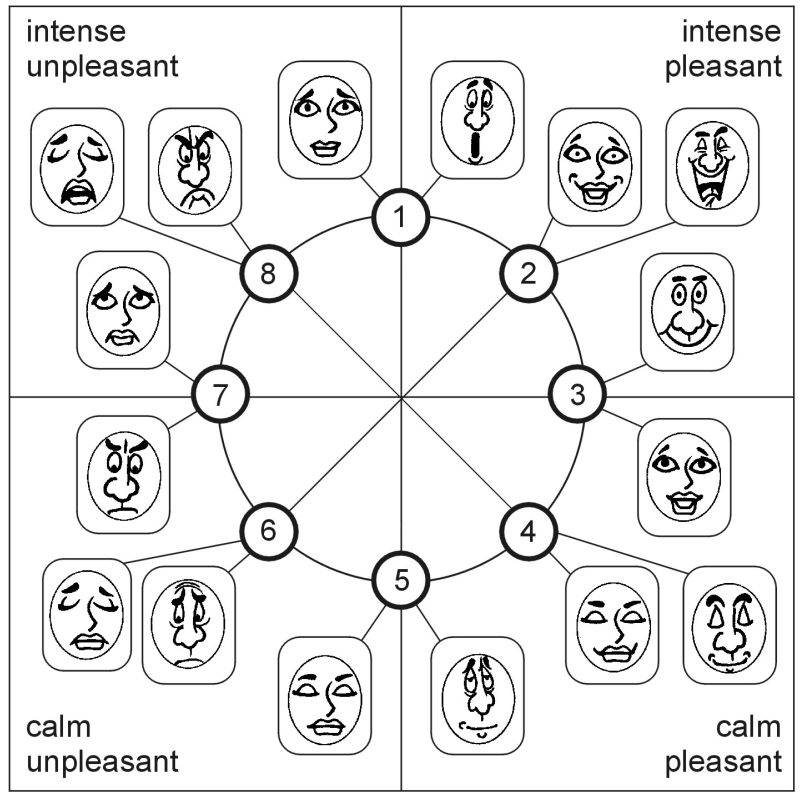
\includegraphics[width=0.5\textwidth]{img/Emocards.png}
        \fonte{\cite{Reijneveld:2003}.}
\end{figure}

% A execução se deu em dezembro de 2021, ainda sem oferecer acesso aos participantes para que eles avaliassem os artefados produzidos pelos geradores implementados em ambas as ferramentas.
% Em relação aos geradores da ERtext, os mesmos foram desativados dentro do ambiente controlado que distribuído.
% Para os geradores da brModelo foi apenas orientado que não era necessário fazer a transformação do modelo conceitual para o lógico ou físico. 
% Isso se deu em razão de tentarmos replicar o experimento anterior visando comparar resultados e, por conta do tempo disponível ser limitado, isso poderia tornar somar mais uma ameaça aos resultados, já que demandaria mais esforço para realizar as tarefas adicionais.
The execution took place in December 2021, still without offering access to the participants so that they could evaluate the artifacts produced by the generators implemented in both tools.
On the one hand, regarding the ERtext generators, we deactivated them within the controlled environment that we distributed.
%Regarding the ERtext generators, they were deactivated within the controlled environment that was distributed.
On the other hand, for the brModelo generators, we only advised that it was not required to transform the conceptual model into a logical or physical one.
%For the brModelo generators, it was only advised that it was not necessary to transform the conceptual model into a logical or physical one.
Hence, this has happened because we tried to replicate the previous experiment to compare the results. 
Also, given the limited time available, this could add another threat to the results, as it would require more effort to perform the additional tasks.
%This was due to the fact that we tried to replicate the previous experiment in order to compare results and, due to the limited time available, this could add another threat to the results, as it would require more effort to perform the additional tasks.

%###########################################################
\subsubsection{Results Analysis}
%###########################################################

% Esta seção apresenta os resultados obtidos da execução do \ac{ex2}.
% Os dados utilizados estão disponíveis em um repositório\footnote{: link do repositório ex2 no Zenodo.} público na plataforma Zenodo.
% Todos os testes estatísticos foram realizados com apoio da linguagem R em conjunto com a IDE RStudio. 
% Os scripts para este experimento estão disponíveis de forma pública em um repositório\footnote{\url{https://github.com/JonnathanRiquelmo/misc/blob/main/some-scripts.r}}, portanto desta forma qualquer pessoa pode, além de consultar todos os dados brutos, executá-los localmente e verificar os resultados.
This section presents the results obtained from the execution of \ac{ex2}.
The data used is available in a public repository\footnote{Available at: \url{https://doi.org/10.5281/zenodo.6416356}.} on the Zenodo platform.
All statistical tests were performed with the support of the R language with the IDE RStudio.
The scripts for this experiment are publicly available in a repository\footnote{Example available at: \url{https://github.com/JonnathanRiquelmo/SE-Masters-Thesis/blob/main/hypothesis-tests.r}.}. 
Hence, anyone can run it locally and verify their results beyond also querying all the raw data.
%so this way anyone can, in addition to querying all the raw data, running it locally, and verifying the results.

% Levamos em consideração as mesmas hipóteses anteriores, relacionadas ao esforço (tempo) necessário e efetividade (qualidade) alcançada pelos modelos feitos.
% Para a avaliação referente ao esforço foram utilizados o teste de normalidade Shapiro-Wilk, em razão da amostra ter menos de trinta (30) elementos, e o Teste T pareado para amostras dependentes, em que foi levado em consideração os tempos coletados durante a execução das atividades de modelagem do experimento.
We bore in mind the same previous hypotheses related to the effort (time) needed and effectiveness (quality) achieved by the models created.
%We took into account the same previous hypotheses, related to the effort (time) needed and effectiveness (quality) achieved by the models made.
For the evaluation regarding the effort, once the sample had less than thirty (30) elements, we used the Shapiro-Wilk normality test.
Otherside the paired T-Test for dependent samples, when we considered the effort spent collected during the execution of the modeling activities.
%For the evaluation regarding the effort, the Shapiro-Wilk normality test was used, due to the sample having less than thirty (30) elements, and the paired T Test for dependent samples, in which the times collected during the execution of the modeling activities were taken into account.

% O método Shapiro-Wilk testa a hipótese nula de que uma distribuição é normal, mediante o cálculo do valor $W$, onde após é então verificado na tabela do teste\footnote{\url{ http://www.uel.br/projetos/experimental/pages/arquivos/Probabilidades\_Shapiro.pdf }} se ocorre a rejeição ou aceitação da hipótese. 
% O cálculo do método Shapiro-Wilk é dado conforme a fórmula da Equação \ref{eq:Shapiro}: 
The Shapiro-Wilk method tests the null hypothesis by calculating whether is a normal distribution revealed by the value $W$.
Then we can verify in the test table\footnote{Available at: \url{ http://www.uel.br/ projects/experimental/pages/arquivos/probabilities\_Shapiro.pdf }} whether the hypothesis is rejected or accepted.
%The Shapiro-Wilk method tests the null hypothesis that a distribution is normal, by calculating the value $W$, after which it is then verified in the test table\footnote{\url{ http://www.uel.br/ projects/experimental/pages/arquivos/probabilities\_Shapiro.pdf }} if the hypothesis is rejected or accepted.
The calculation of the Shapiro-Wilk method is given according to the formula of Equation \ref{eq:Shapiro}:

\begin{equation}
\label{eq:Shapiro}
%\[ 
W = \frac{\left(\sum_{i=1}^{n} a_ix_{(i)}\right)^2}{\sum_{i=1}^{n}\left(x_i -\overline{x}\right)} 
%\]
\end{equation}

% Uma forma simplificada do Teste T pareado para amostras dependentes
% se dá conforme a fórmula da Equação \ref{eq:TestT}:
A simplified form of the Paired T-Test for dependent samples
is given according to the formula of Equation \ref{eq:TestT}:

\begin{equation}
\label{eq:TestT}
%\[ 
t = \frac{m}{s/\sqrt{n}} 
%\]
\end{equation}

% Nesta fórmula o \textit{\textbf{m}} e o \textit{\textbf{s}} são a média e o desvio padrão da diferença (\textbf{\textit{d}}), respectivamente. 
% O \textit{\textbf{n}} corresponde ao tamanho de \textit{\textbf{d}}, ou seja, o tamanho da amostra.
% Este teste de hipótese é usado para comparar as médias de duas amostras relacionadas, ou seja, quando se possui dois valores (ou pares de valores) para uma mesma amostra. 
% Contudo, para comparar as médias dos dois conjuntos de dados emparelhados, as diferenças entre todos os pares precisaram ser calculadas primeiro.
% O nível de significância alfa ($\alpha$) utilizado foi de cinco por cento (5\%).
In this formula, \textit{\textbf{m}} and \textit{\textbf{s}} are the mean and standard deviation of the difference (\textbf{\textit{d}}), respectively.
The \textit{\textbf{n}} corresponds to the size of \textit{\textbf{d}}, that is, the size of the sample.
We used this hypothesis test to compare the means of two related samples, \textit{i.e.}, when you have two values (or pairs of values) for the same sample.
%This hypothesis test is used to compare the means of two related samples, that is, when you have two values (or pairs of values) for the same sample.
However, to compare the means of the two paired data sets, the differences between all pairs had to be calculated first.
The alpha significance level ($\alpha$) used was five percent (5\%).

% Para os testes da efetividade foram adotados os mesmos métodos estatísticos, porém ao invés do uso da métrica de tempo gasto nas atividades, foi necessário outra grandeza.
% Sendo assim, foram realizados novamente cálculos para uma medida F1, conforme também descrito anteriormente na Seção \ref{ssec_experiments:preliminary_planning}.
We adopted the same statistical methods for the effectiveness tests, but instead of using the effort spent (time) measure on activities, we used another magnitude.
%For the effectiveness tests, the same statistical methods were adopted, but instead of using the metric of time spent on activities, another magnitude was needed.
Therefore, we performed calculations again for an F1 measure, as described previously in Section \ref{ssec_experiments:preliminary_planning}.
%Therefore, calculations were performed again for an F1 measure, as also described previously in Section \ref{ssec_experiments:preliminary_planning}.


% A partir dos valores brutos dos tempos foi calculada a diferença para ser possível realizar o teste de normalidade Shapiro-Wilk.
% Por ser um teste estatístico, esta técnica tem como produto a medida do valor-$p$.
% Para este teste foi adotado um nível de significância $\alpha$~=~5\%. 
% Isso significa que se o valor-$p$ for menor que 5\% ($p$ < 0.05), a hipótese nula de que a distribuição é normal deve ser rejeitada.
From the raw time values, the difference was calculated to be able to perform the Shapiro-Wilk normality test.
As it is a statistical test, this technique has as its product the measure of the $p$-value.
A significance level of $\alpha$~=~5\% was adopted for this test.
Hence, through this, if the $p$-value is less than 5\% ($p$ < 0.05), we must reject the null hypothesis since the distribution is not normal.
%This means that if the $p$-value is less than 5\% ($p$ < 0.05), the null hypothesis that the distribution is normal must be rejected.

% Após os cálculos com o conjunto das diferenças dos tempos chegou-se a um valor-$p$ de 0.5991.
% Como valor-$p$ \textgreater $\alpha$, a hipótese nula foi aceita, concluindo assim que os dados são normalmente distribuídos.
% Em outras palavras, a diferença entre a amostra de dados e a distribuição normal não é grande o suficiente para ser estatisticamente significativa.
After the calculations with the set of time differences, we reached a $p$-value of 0.5991.
As $p$-value \textgreater $\alpha$, we accepted the null hypothesis, thus concluding that the data are a normal distribution.
%As $p$-value \textgreater $\alpha$, the null hypothesis was accepted, thus concluding that the data are normally distributed.
In other words, the difference between the sample data and the normal distribution is not large enough to be statistically significant.

% É importante ressaltar que quanto maior o valor-$p$, mais ele suporta uma hipótese nula. 
% No caso do resultado obtido a chance de erro do tipo 1 (rejeitar uma hipótese nula que é correta) é muito alta, podendo ser traduzida em 59,91\% (0.5991).
% Ainda em relação ao teste de normalidade, o valor de \textit{W} calculado foi de 0.968, estando dentro do intervalo aceito do valor crítico de 95\%. 
% Isto significa que existe 95\% de chances da amostra ter origem em uma população normal.
It is important to note that the higher the $p$-value, the more it supports a null hypothesis.
In the case of the result obtained, the chance of a type 1 error (rejecting a correct null hypothesis) is very high, which we can translate into 59.91\% (0.5991).
%In the case of the result obtained, the chance of a type 1 error (rejecting a null hypothesis that is correct) is very high, which can be translated into 59.91\% (0.5991).
Still, about the normality test, we calculated the value of \textit{W} resulting 0.968, being within the range of the critical value accepted of 95\%.
%Still in relation to the normality test, the value of \textit{W} calculated was 0.968, being within the accepted range of the critical value of 95\%.
So this means that there is a 95\% chance that the sample comes from a  population considered normal.
%This means that there is a 95\% chance that the sample comes from a normal population.

% Tendo sido a amostra testada quanto à sua normalidade, foi possível realizar o teste da primeira hipótese estabelecida neste experimento. 
% No teste T pareado para amostras dependentes foi utilizado um nível de significância $\alpha$~=~5\%, com o qual se chegou a uma medida de 0.3492 para o valor-$p$. 
Once we tested the sample for normality, it was possible to test the first hypothesis established in this experiment.
In the paired T-test for dependent samples, we used a significance level of $\alpha$~=~5\%, which reached a measure of 0.3492 for the $p$-value.

% Por ser um teste bicaudal, ou seja, que inclui uma igualdade na sua hipótese nula, esse valor-$p$ não mostra evidências suficientes para garantir a rejeição da afirmativa de $H_0 : \mu Time_G = \mu Time_T$.
% Em resumo, a média dos valores da abordagem gráfica (brModelo) é considerada similar à média da população da abordagem textual (ERtext).
% Em outras palavras, a diferença entre as médias da brModelo e da ERtext não é grande o suficiente para ser estatisticamente significativa.
% A Figura \ref{fig:boxplotTempo2} exibe um gráfico boxplot com a variação observada dos dados obtidos. 
As it is a two-tailed test, that is, it includes an equality in its null hypothesis, this $p$-value does not show enough evidence to guarantee the rejection of the statement of $H_0 : \mu Time_G = \mu Time_T$.
In short, we considered the average of the values of the graphical approach (brModelo) similar to the textual one (ERtext).
%In short, the average of the values of the graphical approach (brModelo) is considered similar to the average of the population of the textual approach (ERtext).
In other words, the difference between the brModelo and ERtext means is not large enough to be statistically significant.
Figure \ref{fig:boxplotTempo2} shows a box-plot with the observed variation of the data obtained.
%Figure \ref{fig:boxplotTime2} displays a box-plot plot with the observed variation of the data obtained.

\begin{figure}[!htb]
        \centering
        \caption{Box-plot - Effort per treatments in EX2.}
        \label{fig:boxplotTempo2}
        \begin{filecontents*}{data2.csv}
24,24,28,28,29,30,30,30,31,33,35,38,38,44,45,46,46,46,53,58,61,70,74,90,102
21,23,25,29,30,30,31,32,35,36,40,40,43,44,47,50,50,55,55,55,67,74,93,93,171
\end{filecontents*}

\makeatletter
\pgfplotsset{
    boxplot/hide outliers/.code={
        \def\pgfplotsplothandlerboxplot@outlier{}%
    }
}
\makeatother

\begin{tikzpicture}
    \pgfplotstableread[col sep=comma]{data2.csv}\csvdata
    % Boxplot groups columns, but we want rows
    \pgfplotstabletranspose\datatransposed{\csvdata} 
    \begin{axis}[
        boxplot/draw direction=y,
        xtick={1, 2},
        ylabel={\scriptsize Time (minutes)},
        xticklabels={{\scriptsize Graphical Treatment}, {\scriptsize Textual Treatment}},
        height=7cm,
        width=10cm,
        % boxplot/draw direction = y,
        % axis x line* = bottom,
        % axis y line = left,
        % enlarge y limits,
        ymajorgrids,
        % xtick = {1, 2},
        % xticklabel style = {align=center, font=\small},
        % xticklabels = {Graphical Treatment, Textual Treatment},
        % ylabel = {Time (minutes)},
        ytick = {15, 30, 45, 60, 75, 90,  105, 120, 135, 150, 165, 180},
        yticklabel style = {font=\scriptsize}
    ]
        \foreach \n in {1,...,2} {
            \addplot+[boxplot, /pgfplots/boxplot/hide outliers, fill, fill opacity=0.4, draw=black] table[y index=\n] {\datatransposed};
        }
    \end{axis}
\end{tikzpicture}


        \fonte{Author.}
\end{figure}

% Para avaliar a hipotése referente a efetividade do uso das abordagens, os artefatos produzidos pelos sujeitos foram avaliados conforme os modelos de referência previamente estabelecidos.
% Como dito, nesta avaliação foi utilizada a medida F1, uma medida proveniente da área de reconhecimento de padrões e recuperação de informação. 
% Essa medida representa a combinação da precisão e revocabilidade observada de um resultado em relação à uma referência.
To assess the hypothesis regarding the effectiveness of using the approaches, we analyzed the artifacts produced by the subjects according to the previously established reference models.
As mentioned, we used in this evaluation the F1 measure, this measure from the area of pattern recognition and information retrieval.
This measure represents the combination of the accuracy observed and the recallability of a result against a reference.

% Após a obtenção dos valores F1 de cada modelo, foi realizado o teste de normalidade Shapiro-Wilk.
% Após os cálculos com o conjunto das diferenças da medida F1 de cada modelo, chegou-se a um valor-$p$ de 0.5166.
% Com este resultado obtido a chance de erro do tipo 1 (rejeitar uma hipótese nula que é correta) pode ser muito alta, podendo ser traduzida em 51,66\% (0.5166).
After obtaining the F1 values of each model, we performed the Shapiro-Wilk normality test.
After the calculations with the set of differences of the F1 measure of each model, we reached a $p$-value of 0.5166.
With this result obtained, the chance of a type 1 error (rejecting a correct null hypothesis) can be very high, which we can translate into 51.66\% (0.5166).

% Como o valor-$p$ \textgreater $\alpha$, a hipótese nula foi aceita, constatando assim que os dados são normalmente distribuídos, isto é, a diferença entre a amostra de dados e uma distribuição normal não é grande o suficiente para ser estatisticamente significativa.
As the value-$p$ \textgreater $\alpha$, we accepted the null hypothesis, thus noting that the data are a normal distribution, \textit{i.e.}, the difference between the sample of data and normal distribution is not large enough to be statistically significant.
%As the value-$p$ \textgreater $\alpha$, the null hypothesis was accepted, thus noting that the data are normally distributed, that is, the difference between the sample of data and a normal distribution is not large enough to be statistically significant.

% Após a amostra ser testada quanto à sua normalidade, foi realizado o teste da segunda hipótese definida, relativa a efetividade (qualidade) das abordagens. 
% Desta vez, no teste T pareado para amostra dependentes, novamente foi utilizado um nível de significância $\alpha$~=~5\%, com o qual se chegou a uma medida de 0.2147 para o valor-$p$. 
After we tested the sample for normality, we performed the test of the second hypothesis defined concerning the effectiveness (quality) of the approaches.
%After the sample was tested for normality, the test of the second defined hypothesis was performed, concerning the effectiveness (quality) of the approaches.
This time, in the paired T-test for dependent samples, we used a significance level $\alpha$~=~5\% again, with which we reached a measure of 0.2147 for the $p$-value.
%This time, in the paired T-test for dependent samples, a significance level $\alpha$~=~5\% was used again, with which a measure of 0.2147 was reached for the $p$-value.

% Pela afirmativa original incluir uma igualdade, caracterizando também este teste como bicaudal, chegou-se a conclusão que o valor-$p$ calculado demonstra que não há evidências suficientes para garantir a rejeição da afirmativa da hipótese nula original, denotada como $H_0 : \mu Effectiveness_G = \mu Effectiveness_T$.
% Logo, a hipótese nula de que as abordagens possuem efetividades iguais é aceita, pois segundo o teste a diferença média da medida F1 entre os tratamentos não é estatisticamente significativa.
% A Figura \ref{tab:ResultsModelosGeral2} apresenta as medidas médias dos valores avaliados, e também fornecem a possibilidade para a realização de uma análise de dispersão.
By the original statement including equality, also characterizing this test as two-tailed, we concluded that the calculated $p$-value demonstrates that there is not enough evidence to guarantee the rejection of the statement of the original null hypothesis, denoted as $H_0 : \mu Effectiveness_G = \mu Effectiveness_T$.
%By the original statement including an equality, also characterizing this test as two-tailed, it was concluded that the calculated value-$p$ demonstrates that there is not enough evidence to guarantee the rejection of the statement of the original null hypothesis, denoted as $H_0 : \mu Effectiveness_G = \mu Effectiveness_T$.
Therefore, we accepted the null hypothesis that the approaches have equal effectiveness because, in accord with the test, the mean difference of the F1 measure between the treatments is not statistically significant.
%Therefore, the null hypothesis that the approaches have equal effectiveness is accepted, because according to the test, the mean difference of the F1 measure between the treatments is not statistically significant.
Table \ref{tab:ResultsModelosGeral2} presents the basic statistical measures of the values evaluated, providing means for dispersion analysis.
%Table \ref{tab:ResultsModelosGeral2} presents the average measures of the evaluated values, and also provides the possibility to carry out a dispersion analysis.

\rowcolors{1}{gray!15}{white}
\begin{table}[!htb]
    \caption{Measures of the conceptual data models produced in EX2.}
    \label{tab:ResultsModelosGeral2}
    \centering
    % \scriptsize
    \tiny
    \begin{tabular}{l|ccccc|ccccc}%{l|ccccc|ccccc}
    \bottomrule
    \rowcolor[HTML]{C0C0C0}
    \multicolumn{1}{l}{} &
    \multicolumn{5}{c|}{\textbf{Graphical Treatment}} &
    \multicolumn{5}{c}{\textbf{Textual Treatment}}
    \\ 
    \hline
    \rowcolor[HTML]{C0C0C0}
    \textbf{Measure} & \textbf{MI} & \textbf{RI} & \textbf{P(\%)} & \textbf{R(\%)} & \textbf{F1(\%)} &
    \textbf{MI} & \textbf{RI} & \textbf{P(\%)} & \textbf{R(\%)} & \textbf{F1(\%)}
    \\
    \hline
Maximum	&	49.00	&	44.00	&	93.75	&	92.50	&	91.67	&	65.00	&	45.00	&	94.74	&	92.68	&	91.14	\\
3\textdegree Quartile	&	46.00	&	39.00	&	88.89	&	85.42	&	86.02	&	47.00	&	38.00	&	89.19	&	87.80	&	87.06	\\
Average	&	41.08	&	35.20	&	85.88	&	78.57	&	81.74	&	44.64	&	36.48	&	83.24	&	83.35	&	82.81	\\
Median	&	43.00	&	36.00	&	86.05	&	77.50	&	81.32	&	44.00	&	36.00	&	85.37	&	83.67	&	84.71	\\
1\textdegree Quartile	&	36.00	&	31.00	&	84.78	&	75.00	&	79.12	&	40.00	&	34.00	&	81.82	&	79.59	&	78.72	\\
Minimum	&	27.00	&	23.00	&	71.43	&	57.50	&	68.66	&	34.00	&	32.00	&	58.46	&	69.39	&	69.47	\\
Variance	&	34.63	&	23.84	&	20.21	&	72.57	&	26.91	&	59.59	&	10.25	&	102.43	&	34.72	&	37.18	\\
SD	&	5.89	&	4.88	&	4.50	&	8.52	&	5.19	&	7.72	&	3.20	&	10.12	&	5.89	&	6.10	\\
    \toprule
\end{tabular}
\begin{tablenotes}
    \scriptsize
    \centering
    \item \textit{Legend: MI = Modeled Items; RI = Relevant Items; P = Precision; \\R = Recall; F1 = F1-Score; SD = Standard Deviation.}
\end{tablenotes}
\fonte{Author.}
\end{table}

% O gráfico boxplot da Figura \ref{fig:boxplotMedidaF2} exibe uma representação visual da medida F1 dos tratamentos aplicados.
% Com base neste gráfico é possível verificar o resultado obtido no teste de hipótese pois a dispersão dos dados não apresenta grande diferença entre as abordagens. 
The box-plot in Figure \ref{fig:boxplotMeasureF2} shows a visual representation of the F1 measurement of the treatments applied.
Based on this graph, it is possible to verify the result obtained in the hypothesis test, as the data dispersion does not present a high difference between the approaches.

\begin{figure}[!htb]
        \centering
        \caption{Box-plot - F1 per treatments in EX2.}
        \label{fig:boxplotMeasureF2}
        \include{img/boxplotMedidaF2}
        \fonte{Author.}
\end{figure}

% A avaliação referente aos atributos de qualidade para as ferramentas é apresentado na Figura \ref{fig:inst3GERALExp2}.
% No geral, o resultado da avaliação feita pelos participantes foi proporcionalmente similar a obtida no experimento anterior. 
% Os destaques desta vez ficaram por conta do atributo de satisfação para a abordagem textual, enquanto os atributos de conformidade e compreensão se sairam melhores na abordagem gráfica. 
% Outro ponto a ser ressaltado é a diferença levemente menor no atributo de produtividade, mas ainda se mantendo em favor da abordagem textual.
Figure~\ref{fig:inst3GERALExp2} shows the evaluation regarding the quality attributes of the tools.
%The evaluation regarding the quality attributes for the tools is shown in Figure~\ref{fig:inst3GERALExp2}.
In general, the evaluation results made by the participants were proportionally similar to that obtained in the previous experiment.
%In general, the result of the evaluation made by the participants was proportionally similar to that obtained in the previous experiment.
The highlights this time was the Satisfaction attribute for the textual approach, while the Conformity and Understanding attributes performed better in the graphical one.
%The highlights this time was the satisfaction attribute for the textual approach, while the conformity and understanding attributes performed better in the graphical approach.
Another point to highlight is the slightly smaller difference in the Productivity attribute, but still in favor of the textual approach.
%Another point to be highlighted is the slightly smaller difference in the productivity attribute, but still in favor of the textual approach.

\begin{figure}[!htb]
    \centering
    \caption{Quality attributes per treatments in EX2.}
    \label{fig:inst3GERALExp2}
    \pgfplotsset{testbar/.style={
        xbar stacked,
        legend cell align=left,
        legend style={
            legend columns=8,
            font=\scriptsize,
            at={(xticklabel cs:1.0)},
            anchor=north east,
            draw=none,
            nodes={scale=1}
            },
        width=10cm,
        axis y line*= none, 
        axis x line*= bottom,
        xmajorgrids = false,
        xmin=0,xmax=25,
        ytick = data,
        yticklabels = {
            {\scriptsize Conformity-ERtext},
            {\scriptsize Conformity-brModelo},
            {\scriptsize Understandability-ERtext}, %Intelligibility
            {\scriptsize Understandability-brModelo},
            {\scriptsize Learnability-ERtext}, %Apprehensibility
            {\scriptsize Learnability-brModelo}, 
            {\scriptsize Operability-ERtext},
            {\scriptsize Operability-brModelo},
            {\scriptsize Quality in Use-ERtext},
            {\scriptsize Quality in Use-brModelo},
            {\scriptsize Productivity-ERtext}, %Performance Efficiency
            {\scriptsize Productivity-brModelo},
            {\scriptsize Satisfaction-ERtext},
            {\scriptsize Satisfaction-brModelo}
        },
        tick align = outside, 
        xtick pos = left,
        xticklabel style = {font=\scriptsize},
        bar width=5mm, 
        y=7mm,
        enlarge y limits={abs=0.450},% 0.5 + 0.5*(y - bar width)/y [TeX.sx #47995]
        nodes near coords,
        nodes near coords align=center,%Move values in bar
        every node near coord/.append style={
            black,
            font=\scriptsize,
            text opacity=1,
            fill=white,
            fill opacity=0.5,
            outer sep=\pgflinewidth
        }
    }}
    \begin{tikzpicture}
    \begin{axis}[testbar] 
    \addplot[pattern color=red,pattern=north east lines] coordinates
        {(0,14)(0,13)(0,12)(0,11)(0,10)(0,9)(0,8)(1,7)(0,6)(0,5)(0,4)(1,3)(0,2)(1,1)};
    \addplot[pattern color=teal,pattern=vertical lines] coordinates
        {(0,14)(0,13)(0,12)(0,11)(2,10)(1,9)(1,8)(2,7)(0,6)(1,5)(1,4)(2,3)(0,2)(1,1)};
    \addplot[pattern color=gray, pattern=grid] coordinates
       {(0,14)(1,13)(1,12)(0,11)(3,10)(3,9)(2,8)(4,7)(2,6)(1,5)(2,4)(2,3)(2,2)(4,1)};
    \addplot[pattern color=magenta, pattern=north west lines] coordinates
       {(6,14)(4,13)(5,12)(5,11)(8,10)(6,9)(6,8)(7,7)(5,6)(2,5)(5,4)(5,3)(4,2)(3,1)};
    \addplot[pattern color=blue, pattern=horizontal lines] coordinates
       {(10,14)(5,13)(8,12)(7,11)(7,10)(9,9)(10,8)(6,7)(11,6)(9,5)(9,4)(9,3)(4,2)(7,1)};
    \addplot[pattern color=green, pattern=crosshatch dots] coordinates
       {(9,14)(15,13)(11,12)(13,11)(5,10)(6,9)(6,8)(5,7)(7,6)(12,5)(8,4)(6,3)(15,2)(9,1)};
    \legend{1-Disagree, 2, 3, 4, 5, 6-Agree}
    \end{axis}
    \end{tikzpicture}
    
% \begin{tikzpicture}
% \begin{axis}[
%     xbar stacked,
%     legend cell align=center,
%     legend style={
%     legend columns=5,
%         at={(xticklabel cs:1.0)},
%         anchor=north east,
%         draw=none
%     },
%     ytick=data,
%     axis y line*=none,
%     axis x line*=bottom,
%     tick label style={font=\small},
%     legend style={font=\small},
%     label style={font=\small},
%     xtick={0,3,6},
%     xticklabel= {},
%     bar width=5mm,
%     ylabel={Questions},
%     yticklabels={P-Q1, T-Q1, P-Q2, T-Q2, P-Q3, T-Q3, P-Q4, T-Q4,P-Q5, T-Q5,P-Q6, T-Q6, P-Q7, T-Q7},
%     xmin=0,
%     xmax=6,
%     area legend,
%     y=6.5mm,
%     enlarge y limits={abs=0.625},
%     nodes near coords,
%     nodes near coords align=center,
%     every node near coord/.append style={
%         black,
%         font=\small,
%         text opacity=.65,
%         fill=white,
%         fill opacity=0.75,
%         outer sep=\pgflinewidth
%     }
% ]
% \addplot[pattern color=red,pattern=horizontal lines] coordinates
% {(0,14)(0,13)(0,12)(0,11) (3,10)(0,9)(0,8) (0,7) (0,6)(0,5)(0,4) (0,3) (0,2) (0,1)};   
% \addplot[pattern color=orange,pattern=grid] coordinates
% {(3,14) (0,13)(0,12)(0,11)(2,10) (1,9)(1,8)(0,7)(3,6)(0,5)(0,4)(3,3) (4,2) (0,1) };  
% \addplot[pattern color = green, pattern=crosshatch dots] coordinates
% {(0,14) (0,13) (3,12)(2,11)(1,10) (3,9)(4,8)(1,7)(3,6)(1,5)(3,4)(2,3)(2,2) (2,1) };   
% \addplot[pattern color=blue, pattern =vertical lines ] coordinates
% {(2,14) (3,13) (2,12)(3,11)(0,10)(2,9)(1,8)(4,7)(0,6)(3,5) (3,4)(1,3)(0,2)(4,1)};   
% \addplot[pattern color=gray, pattern = dots] coordinates
% {(1,14)(3,13)(1,12)(1,11)(0,10)(0,9)(0,8)(1,7) (0,6)(2,5) (0,4)(0,3)(0,2)(0,1) };   
% \legend{1-Disagree, 2, 3, 4, 5-Agree}

% \end{axis}
% \end{tikzpicture}
% \footnotesize
% T-Thoth answers; P-Parsifal answers;






% \begin{tikzpicture}
% \begin{axis}[
%     xbar stacked,
%     legend cell align=left,
%     legend style={
%     legend columns=2,
%         at={(xticklabel cs:1.0)},
%         anchor=north east,
%         draw=none
%     },
%     ytick=data,
%     axis y line*=none,
%     axis x line*=bottom,
%     tick label style={font=\scriptsize},
%     legend style={font=\scriptsize},
%     %legend style={font=\scriptsize,row sep=-0.1cm,/tikz/every odd column/.append style={column sep=0.01cm}},
%     label style={font=\scriptsize},
%     xtick={0,10,...,100},
%     width=\columnwidth,
%     bar width=3.5mm,
%     % xlabel={Frequencia em \%},
%     yticklabels={
%     {Q1 - OC},
%     {Q2 - TD},
%     {Q3 - OC},
%     {Q4 - TD},
%     {Q5 - OC},
%     {Q6 - TD},
%     {Q7 - OC},
%     {Q8 - TD},
%     {Q9 - OC},
%     {Q10 - TD},
%     {Q11 - OC},
%     {Q12 - TD}},
%     xmin=0,
%     xmax=100,
%     area legend,
%     y=5mm,
%     enlarge y limits={abs=0.625},
%     nodes near coords,
%     nodes near coords={\pgfmathprintnumber\pgfplotspointmeta\%},
%     nodes near coords align=center,%Move values in bar
%     every node near coord/.append style={
%         black,
%         font=\footnotesize,
%         text opacity=1,
%         fill=white,
%         fill opacity=0.7,
%         outer sep=\pgflinewidth
%     }
% ]
% \addplot[pattern color=blue,pattern=dots] coordinates
% {(0,0)(0,1)(0,2)(0,3)(0,4)(0,5)(0,6)(0,7)(0,8)(0,9)(0,10)(0,11)};
% \addplot[pattern color=red, pattern=vertical lines] coordinates
% {(4,0)(32,1)(0,2)(9,3)(13,4)(18,5)(0,6)(9,7)(5,8)(5,9)(0,10)(14,11)};
% \addplot[pattern color=cyan, pattern=grid] coordinates
% {(27,0)(9,1)(4,2)(5,3)(23,4)(27,5)(36,6)(23,7)(27,8)(41,9)(46,10)(45,11)};
% \addplot[pattern color=green, pattern=horizontal lines] coordinates
% {(55,0)(32,1)(55,2)(68,3)(41,4)(50,5)(46,6)(64,7)(64,8)(45,9)(36,10)(27,11)};
% \addplot[pattern color=orange, pattern=crosshatch dots] coordinates
% {(14,0)(27,1)(41,2)(18,3)(23,4)(5,5)(18,6)(4,7)(4,8)(9,9)(18,10)(14,11)};
% \legend{Strongly disagree,Disagree,Neither agree nor disagree,Agree,Strongly agree}; 

% \end{axis}  
% \end{tikzpicture}d
    \fonte{Author.}
\end{figure}

% A avaliação referente aos construtores da DSL da abordagem textual, os resultados também seguiram a mesma proporção observada no primeiro experimento.
% Isso nos leva a concluir que de fato é necessário, principalmente, uma reavaliação da representação dos relacionamentos ternários para torná-los mais fáceis de aprender, interpretar e utilizar.
The evaluation results referring to the DSL builders of the textual approach also followed the same proportion observed in the first experiment.
%The evaluation referring to the DSL builders of the textual approach, the results also followed the same proportion observed in the first experiment.
Then leads us to conclude that it is necessary, mainly, to re-execute an evaluation of the representation of the ternary relationships to make them easier to learn, interpret, and use.
%This leads us to conclude that, in fact, it is necessary, mainly, a reassessment of the representation of ternary relationships to make them easier to learn, interpret and use.

\begin{figure}[!htb]
    \centering
    \caption{Evaluation of DSL designers in EX2.}
    \label{fig:inst4GERALExp2}
    \pgfplotsset{testbar/.style={
            xbar stacked,
            legend cell align=left,
            legend style={
                legend columns=6,
                font=\scriptsize,
                at={(xticklabel cs:1.0)},
                anchor=north east,
                draw=none
                },
            width=10cm,
            axis y line*= none, 
            axis x line*= bottom,
            xmajorgrids = false,
            xmin=0,xmax=25,
            ytick = data,
            yticklabels = {
            {\scriptsize Entity}, 
            {\scriptsize Referential Attribute},
            {\scriptsize Descriptive Attribute},
            {\scriptsize Binary Relationship},
            {\scriptsize Ternary Relationship}, 
            {\scriptsize Self-relationship},
            {\scriptsize Cardinality},
            {\scriptsize Generalization}
            },
            tick align = outside, 
            xticklabel style = {font=\scriptsize},
            xtick pos = left,
             bar width=3.5mm, 
             y=6.5mm,
             enlarge y limits={abs=0.450},% 0.5 + 0.5*(y - bar width)/y [TeX.sx #47995] #47995]
            nodes near coords,
            nodes near coords align=center,%Move values in bar
            every node near coord/.append style={
                black,
                font=\scriptsize,
                text opacity=1,
                fill=white,
                fill opacity=0.5,
                outer sep=\pgflinewidth
            }
        }}
    \begin{tikzpicture}
    \begin{axis}[testbar] 
    \addplot[pattern color=red,pattern=north east lines] coordinates
        {(0,8)(0,7)(0,6)(0,5)(0,4)(0,3)(0,2)(0,1)};
    \addplot[pattern color=teal,pattern=vertical lines] coordinates
        {(0,8)(0,7)(0,6)(1,5)(2,4)(1,3)(0,2)(0,1)};   
    \addplot[pattern color=gray, pattern=grid] coordinates
        {(0,8)(0,7)(2,6)(2,5)(5,4)(0,3)(0,2)(3,1)};   
    \addplot[pattern color=magenta, pattern=north west lines] coordinates
        {(3,8)(4,7)(2,6)(0,5)(6,4)(3,3)(0,2)(3,1)};   
    \addplot[pattern color=blue, pattern=horizontal lines] coordinates
        {(4,8)(4,7)(6,6)(11,5)(7,4)(5,3)(5,2)(6,1)}; 
    \addplot[pattern color=green, pattern=crosshatch dots] coordinates
        {(18,8)(17,7)(15,6)(11,5)(5,4)(16,3)(20,2)(13,1)};
    \legend{1-Disagree, 2, 3, 4, 5, 6-Agree}
    \end{axis}
    \end{tikzpicture}

% \begin{figure}[!ht]
% \centering
% \caption{Resultados do formulários de avaliação.}
% \begin{tikzpicture}
% \begin{axis}[
%     xbar stacked,
%     legend cell align=center,
%     legend style={
%     legend columns=5,
%         at={(xticklabel cs:1.0)},
%         anchor=north east,
%         draw=none
%     },
%     ytick=data,
%     axis y line*=none,
%     axis x line*=bottom,
%     tick label style={font=\small},
%     legend style={font=\small},
%     label style={font=\small},
%     xtick={0,5,10},
%     xticklabel= {},
%     bar width=7mm,
%     ylabel={Formulário/Grupo},
%     yticklabels={F1-C, F1-E, F2-C, F2-E, F3-C, F3-E},
%     xmin=0,
%     xmax=10,
%     area legend,
%     y=9mm,
%     enlarge y limits={abs=0.825},
%     nodes near coords,
%     nodes near coords align=center,
%     every node near coord/.append style={
%         black,
%         font=\small,
%         text opacity=.65,
%         fill=white,
%         fill opacity=0.6,
%         outer sep=\pgflinewidth
%     }
% ]
% %NOTA 1
% \addplot[pattern color=red,pattern=horizontal lines] coordinates
% {(0,6)(0,5)(0,4)(0,3)(0,2)(0,1)};
% %NOTA 2
% \addplot[pattern color=orange,pattern=grid] coordinates
% {(1,6)(1,5)(1,4)(0,3)(1,2)(0,1)};   
% \addplot[pattern color = green, pattern=crosshatch dots] coordinates
% % NOTA 3
% {(3,6)(3,5)(5,4)(2,3)(5,2)(1,1)};   
% \addplot[pattern color=blue, pattern =vertical lines ] coordinates
% %NOTA 4
% {(2,6)(3,5)(1,4)(4,3)(3,2)(3,1)};   
% \addplot[pattern color=gray, pattern = dots] coordinates
% %NOTA 5
% {(3,6)(3,5)(2,4)(4,3)(0,2)(6,1)};   
% \legend{1-Disagree, 2, 3, 4, 5-Agree}

% \end{axis}
% \end{tikzpicture}
% \footnotesize
% \label{img:respostas1}
% 	\fonte{O autor.}
% \end{figure}
    \fonte{Author.}
\end{figure}

% Finalmente, chegamos aos instrumentos adicionados para tentar verificar o estado de espírito, ou as emoções causadas, pela execução das atividades com cada abordagem.
% Os resultados das avaliações são dispostas em um circumplexo de Russell.
% É possível observar que em relação ao uso da abordagem textual com a ferramenta ERtext houve uma concentração maior nos quadrantes que dizem respeito aos sentimento de alegria (octantes 1 e 2) e relaxamento (octantes 3 e 4).
Finally, we come to the added instruments trying to verify the state of mind or the emotions caused by the execution of the activities with each approach.
%Finally, we come to the added instruments to try to verify the state of mind, or the emotions caused, by the execution of the activities with each approach.
We arranged the results of the evaluations in Russell's Circumplex. 
%The results of the evaluations are arranged in a Russell circumplex. 
It is possible to observe that regarding the use of the textual approach with the ERtext tool, there was a greater concentration in the quadrants that concern feelings of happiness (Octants 1 and 2) and relaxation (Octants 3 and 4).

% Esses dois quadrantes concentraram um total de vinte (20) respondentes.
% Ainda, houve a distribuição de três (3) partipantes que expressaram sentimentos relacionados a tristeza (octantes 5 e 6), e dois (2) sujeitos que demonstraram se identificarem com os Emocards relacionados ao quadrante que diz respeito a emoções de irritabilidade (octantes 7 e 8).
% A Figura \ref{fig:Emocards1_alt} apresenta a distribuição dos sujeitos por cada octante previsto no método Emocards, e que utilizaram a abordagem textual.
These two quadrants concentrated a total of twenty (20) respondents.
Also, there were a distribution of three (3) participants who expressed feelings related to sadness (Octants 5 and 6) and two (2) subjects who demonstrated identification with the Emocards related to the quadrant that concerns emotions of irritability (Octants 7 and 8).
Figure \ref{fig:Emocards1_alt} presents the distribution of subjects for each octant predicted in the Emocards method, which used the textual approach.

\begin{figure}[!htb]
    \centering
    \caption{EX2 Emocards - ERtext.}
    \label{fig:Emocards1_alt}
    

\tikzset{every picture/.style={line width=0.75pt}} %set default line width to 0.75pt        

\begin{tikzpicture}[x=0.75pt,y=0.75pt,yscale=-1,xscale=1]
%uncomment if require: \path (0,389); %set diagram left start at 0, and has height of 389

%Flowchart: Or [id:dp3592995680476845] 
\draw  [color={rgb, 255:red, 74; green, 74; blue, 74 }  ,draw opacity=1 ] (182.64,181.1) .. controls (182.64,116.34) and (252,63.84) .. (337.55,63.84) .. controls (423.11,63.84) and (492.46,116.34) .. (492.46,181.1) .. controls (492.46,245.86) and (423.11,298.36) .. (337.55,298.36) .. controls (252,298.36) and (182.64,245.86) .. (182.64,181.1) -- cycle ; \draw  [color={rgb, 255:red, 74; green, 74; blue, 74 }  ,draw opacity=1 ] (182.64,181.1) -- (492.46,181.1) ; \draw  [color={rgb, 255:red, 74; green, 74; blue, 74 }  ,draw opacity=1 ] (337.55,63.84) -- (337.55,298.36) ;
%Straight Lines [id:da30798451784186187] 
\draw [color={rgb, 255:red, 74; green, 74; blue, 74 }  ,draw opacity=1 ] [dash pattern={on 3.75pt off 3pt on 2.25pt off 1.5pt}]  (188.22,68.06) -- (486.88,294.14) ;
%Straight Lines [id:da7804870395610348] 
\draw [color={rgb, 255:red, 74; green, 74; blue, 74 }  ,draw opacity=1 ] [dash pattern={on 3.75pt off 3pt on 2.25pt off 1.5pt}]  (486.88,68.06) -- (188.22,294.14) ;
%Shape: Rectangle [id:dp23344423808181314] 
\draw  [color={rgb, 255:red, 128; green, 128; blue, 128 }  ,draw opacity=1 ] (133.68,26.77) -- (541.42,26.77) -- (541.42,335.43) -- (133.68,335.43) -- cycle ;

% Text Node
\draw  [color={rgb, 255:red, 0; green, 0; blue, 0 }  ,draw opacity=1 ][fill={rgb, 255:red, 100; green, 12; blue, 176 }  ,fill opacity=1 ]  (400.79,192.22) -- (421.79,192.22) -- (421.79,206.22) -- (400.79,206.22) -- cycle  ;
\draw (411.29,199.22) node  [font=\tiny,color={rgb, 255:red, 255; green, 255; blue, 255 }  ,opacity=1 ] [align=left] {S02};
% Text Node
\draw  [color={rgb, 255:red, 0; green, 0; blue, 0 }  ,draw opacity=1 ][fill={rgb, 255:red, 55; green, 100; blue, 4 }  ,fill opacity=1 ]  (342.09,203.64) -- (362.09,203.64) -- (362.09,217.64) -- (342.09,217.64) -- cycle  ;
\draw (352.09,210.64) node  [font=\tiny,color={rgb, 255:red, 255; green, 255; blue, 255 }  ,opacity=1 ] [align=left] {S11};
% Text Node
\draw  [color={rgb, 255:red, 0; green, 0; blue, 0 }  ,draw opacity=1 ][fill={rgb, 255:red, 176; green, 132; blue, 58 }  ,fill opacity=1 ]  (366.87,163.61) -- (387.87,163.61) -- (387.87,177.61) -- (366.87,177.61) -- cycle  ;
\draw (377.37,170.61) node  [font=\tiny,color={rgb, 255:red, 255; green, 255; blue, 255 }  ,opacity=1 ] [align=left] {S03};
% Text Node
\draw  [color={rgb, 255:red, 0; green, 0; blue, 0 }  ,draw opacity=1 ][fill={rgb, 255:red, 100; green, 12; blue, 176 }  ,fill opacity=1 ]  (461.95,197.33) -- (482.95,197.33) -- (482.95,211.33) -- (461.95,211.33) -- cycle  ;
\draw (472.45,204.33) node  [font=\tiny,color={rgb, 255:red, 255; green, 255; blue, 255 }  ,opacity=1 ] [align=left] {S13};
% Text Node
\draw  [color={rgb, 255:red, 0; green, 0; blue, 0 }  ,draw opacity=1 ][fill={rgb, 255:red, 183; green, 0; blue, 0 }  ,fill opacity=0.9 ]  (294.12,96.99) -- (315.12,96.99) -- (315.12,110.99) -- (294.12,110.99) -- cycle  ;
\draw (304.62,103.99) node  [font=\tiny,color={rgb, 255:red, 255; green, 255; blue, 255 }  ,opacity=1 ] [align=left] {S09};
% Text Node
\draw  [color={rgb, 255:red, 0; green, 0; blue, 0 }  ,draw opacity=1 ][fill={rgb, 255:red, 100; green, 12; blue, 176 }  ,fill opacity=1 ]  (371.22,187.92) -- (392.22,187.92) -- (392.22,201.92) -- (371.22,201.92) -- cycle  ;
\draw (381.72,194.92) node  [font=\tiny,color={rgb, 255:red, 255; green, 255; blue, 255 }  ,opacity=1 ] [align=left] {S01};
% Text Node
\draw  [color={rgb, 255:red, 0; green, 0; blue, 0 }  ,draw opacity=1 ][fill={rgb, 255:red, 100; green, 12; blue, 176 }  ,fill opacity=1 ]  (405.75,214.64) -- (426.75,214.64) -- (426.75,228.64) -- (405.75,228.64) -- cycle  ;
\draw (416.25,221.64) node  [font=\tiny,color={rgb, 255:red, 255; green, 255; blue, 255 }  ,opacity=1 ] [align=left] {S05};
% Text Node
\draw  [color={rgb, 255:red, 0; green, 0; blue, 0 }  ,draw opacity=1 ][fill={rgb, 255:red, 17; green, 0; blue, 185 }  ,fill opacity=1 ]  (305.76,216.61) -- (326.76,216.61) -- (326.76,230.61) -- (305.76,230.61) -- cycle  ;
\draw (316.26,223.61) node  [font=\tiny,color={rgb, 255:red, 255; green, 255; blue, 255 }  ,opacity=1 ] [align=left] {S04};
% Text Node
\draw  [color={rgb, 255:red, 0; green, 0; blue, 0 }  ,draw opacity=1 ][fill={rgb, 255:red, 176; green, 132; blue, 58 }  ,fill opacity=1 ]  (424.83,159.33) -- (445.83,159.33) -- (445.83,173.33) -- (424.83,173.33) -- cycle  ;
\draw (435.33,166.33) node  [font=\tiny,color={rgb, 255:red, 255; green, 255; blue, 255 }  ,opacity=1 ] [align=left] {S15};
% Text Node
\draw  [color={rgb, 255:red, 0; green, 0; blue, 0 }  ,draw opacity=1 ][fill={rgb, 255:red, 100; green, 12; blue, 176 }  ,fill opacity=1 ]  (435.18,206.39) -- (456.18,206.39) -- (456.18,220.39) -- (435.18,220.39) -- cycle  ;
\draw (445.68,213.39) node  [font=\tiny,color={rgb, 255:red, 255; green, 255; blue, 255 }  ,opacity=1 ] [align=left] {S06};
% Text Node
\draw  [color={rgb, 255:red, 0; green, 0; blue, 0 }  ,draw opacity=1 ][fill={rgb, 255:red, 100; green, 12; blue, 176 }  ,fill opacity=1 ]  (439.6,230.11) -- (460.6,230.11) -- (460.6,244.11) -- (439.6,244.11) -- cycle  ;
\draw (450.1,237.11) node  [font=\tiny,color={rgb, 255:red, 255; green, 255; blue, 255 }  ,opacity=1 ] [align=left] {S08};
% Text Node
\draw  [color={rgb, 255:red, 0; green, 0; blue, 0 }  ,draw opacity=1 ][fill={rgb, 255:red, 176; green, 132; blue, 58 }  ,fill opacity=1 ]  (394.61,157.99) -- (415.61,157.99) -- (415.61,171.99) -- (394.61,171.99) -- cycle  ;
\draw (405.11,164.99) node  [font=\tiny,color={rgb, 255:red, 255; green, 255; blue, 255 }  ,opacity=1 ] [align=left] {S10};
% Text Node
\draw  [color={rgb, 255:red, 0; green, 0; blue, 0 }  ,draw opacity=1 ][fill={rgb, 255:red, 207; green, 0; blue, 118 }  ,fill opacity=0.81 ]  (366.18,93.21) -- (387.18,93.21) -- (387.18,107.21) -- (366.18,107.21) -- cycle  ;
\draw (376.68,100.21) node  [font=\tiny,color={rgb, 255:red, 255; green, 255; blue, 255 }  ,opacity=1 ] [align=left] {S14};
% Text Node
\draw  [color={rgb, 255:red, 0; green, 0; blue, 0 }  ,draw opacity=1 ][fill={rgb, 255:red, 176; green, 132; blue, 58 }  ,fill opacity=1 ]  (406.53,137.78) -- (427.53,137.78) -- (427.53,151.78) -- (406.53,151.78) -- cycle  ;
\draw (417.03,144.78) node  [font=\tiny,color={rgb, 255:red, 255; green, 255; blue, 255 }  ,opacity=1 ] [align=left] {S12};
% Text Node
\draw  [color={rgb, 255:red, 0; green, 0; blue, 0 }  ,draw opacity=1 ][fill={rgb, 255:red, 100; green, 12; blue, 176 }  ,fill opacity=1 ]  (429.94,184.66) -- (450.94,184.66) -- (450.94,198.66) -- (429.94,198.66) -- cycle  ;
\draw (440.44,191.66) node  [font=\tiny,color={rgb, 255:red, 255; green, 255; blue, 255 }  ,opacity=1 ] [align=left] {S07};
% Text Node
\draw  [color={rgb, 255:red, 255; green, 255; blue, 255 }  ,draw opacity=1 ][fill={rgb, 255:red, 0; green, 0; blue, 0 }  ,fill opacity=1 ]  (337.55, 63.84) circle [x radius= 13.73, y radius= 13.73]   ;
\draw (337.55,63.84) node  [font=\normalsize,color={rgb, 255:red, 255; green, 255; blue, 255 }  ,opacity=1 ] [align=left] {\textbf{1}};
% Text Node
\draw  [color={rgb, 255:red, 255; green, 255; blue, 255 }  ,draw opacity=1 ][fill={rgb, 255:red, 0; green, 0; blue, 0 }  ,fill opacity=1 ]  (447.88, 96.18) circle [x radius= 13.73, y radius= 13.73]   ;
\draw (447.88,96.18) node  [font=\normalsize,color={rgb, 255:red, 255; green, 255; blue, 255 }  ,opacity=1 ] [align=left] {\textbf{2}};
% Text Node
\draw  [color={rgb, 255:red, 255; green, 255; blue, 255 }  ,draw opacity=1 ][fill={rgb, 255:red, 0; green, 0; blue, 0 }  ,fill opacity=1 ]  (492.46, 181.1) circle [x radius= 13.73, y radius= 13.73]   ;
\draw (492.46,181.1) node  [font=\normalsize,color={rgb, 255:red, 255; green, 255; blue, 255 }  ,opacity=1 ] [align=left] {\textbf{3}};
% Text Node
\draw  [color={rgb, 255:red, 255; green, 255; blue, 255 }  ,draw opacity=1 ][fill={rgb, 255:red, 0; green, 0; blue, 0 }  ,fill opacity=1 ]  (447.05, 262.88) circle [x radius= 13.73, y radius= 13.73]   ;
\draw (447.05,262.88) node  [font=\normalsize,color={rgb, 255:red, 255; green, 255; blue, 255 }  ,opacity=1 ] [align=left] {\textbf{4}};
% Text Node
\draw  [color={rgb, 255:red, 255; green, 255; blue, 255 }  ,draw opacity=1 ][fill={rgb, 255:red, 0; green, 0; blue, 0 }  ,fill opacity=1 ]  (337.55, 298.36) circle [x radius= 13.73, y radius= 13.73]   ;
\draw (337.55,298.36) node  [font=\normalsize,color={rgb, 255:red, 255; green, 255; blue, 255 }  ,opacity=1 ] [align=left] {\textbf{5}};
% Text Node
\draw  [color={rgb, 255:red, 255; green, 255; blue, 255 }  ,draw opacity=1 ][fill={rgb, 255:red, 0; green, 0; blue, 0 }  ,fill opacity=1 ]  (228.16, 263.49) circle [x radius= 13.73, y radius= 13.73]   ;
\draw (228.16,263.49) node  [font=\normalsize,color={rgb, 255:red, 255; green, 255; blue, 255 }  ,opacity=1 ] [align=left] {\textbf{6}};
% Text Node
\draw  [color={rgb, 255:red, 255; green, 255; blue, 255 }  ,draw opacity=1 ][fill={rgb, 255:red, 0; green, 0; blue, 0 }  ,fill opacity=1 ]  (182.64, 181.1) circle [x radius= 13.73, y radius= 13.73]   ;
\draw (182.64,181.1) node  [font=\normalsize,color={rgb, 255:red, 255; green, 255; blue, 255 }  ,opacity=1 ] [align=left] {\textbf{7}};
% Text Node
\draw  [color={rgb, 255:red, 255; green, 255; blue, 255 }  ,draw opacity=1 ][fill={rgb, 255:red, 0; green, 0; blue, 0 }  ,fill opacity=1 ]  (229.45, 95.43) circle [x radius= 13.73, y radius= 13.73]   ;
\draw (229.45,95.43) node  [font=\normalsize,color={rgb, 255:red, 255; green, 255; blue, 255 }  ,opacity=1 ] [align=left] {\textbf{8}};
% Text Node
\draw (112.89,231.39) node [anchor=north west][inner sep=0.75pt]  [rotate=-270] [align=left] {DISPLEASURE};
% Text Node
\draw (292.08,5.96) node [anchor=north west][inner sep=0.75pt]   [align=left] {ACTIVATION};
% Text Node
\draw (281.58,342.71) node [anchor=north west][inner sep=0.75pt]   [align=left] {DEACTIVATION};
% Text Node
\draw (562.94,136.89) node [anchor=north west][inner sep=0.75pt]  [rotate=-90] [align=left] {PLEASURE};
% Text Node
\draw (150.9,160.23) node [anchor=north west][inner sep=0.75pt]  [font=\scriptsize,rotate=-301.49] [align=left] {upset distressed};
% Text Node
\draw (247.79,60.45) node [anchor=north west][inner sep=0.75pt]  [font=\scriptsize,rotate=-341.6] [align=left] {tense jittery};
% Text Node
\draw (359.94,41.46) node [anchor=north west][inner sep=0.75pt]  [font=\scriptsize,rotate=-17.34] [align=left] {excited ebullient};
% Text Node
\draw (485.75,96.5) node [anchor=north west][inner sep=0.75pt]  [font=\scriptsize,rotate=-59.2] [align=left] {elated happy};
% Text Node
\draw (470.66,265.95) node [anchor=north west][inner sep=0.75pt]  [font=\scriptsize,rotate=-301.93] [align=left] {serene contented};
% Text Node
\draw (373.68,306.2) node [anchor=north west][inner sep=0.75pt]  [font=\scriptsize,rotate=-343.65] [align=left] {placid calm};
% Text Node
\draw (241.21,287.33) node [anchor=north west][inner sep=0.75pt]  [font=\scriptsize,rotate=-18.04] [align=left] {tired lethargic};
% Text Node
\draw (169.56,210.51) node [anchor=north west][inner sep=0.75pt]  [font=\scriptsize,rotate=-56.13] [align=left] {sad gloomy};
% Text Node
\draw (455,317) node [anchor=north west][inner sep=0.75pt]  [font=\footnotesize] [align=left] {calm pleasant};
% Text Node
\draw (136.67,317) node [anchor=north west][inner sep=0.75pt]  [font=\footnotesize] [align=left] {calm unpleasant};
% Text Node
\draw (136.67,32.78) node [anchor=north west][inner sep=0.75pt]  [font=\footnotesize] [align=left] {intense unpleasant};
% Text Node
\draw (442,32.78) node [anchor=north west][inner sep=0.75pt]  [font=\footnotesize] [align=left] {intense pleasant};
% Text Node
\draw  [color={rgb, 255:red, 0; green, 0; blue, 0 }  ,draw opacity=1 ][fill={rgb, 255:red, 55; green, 100; blue, 4 }  ,fill opacity=1 ]  (366.83,226.83) -- (387.83,226.83) -- (387.83,240.83) -- (366.83,240.83) -- cycle  ;
\draw (377.33,233.83) node  [font=\tiny,color={rgb, 255:red, 255; green, 255; blue, 255 }  ,opacity=1 ] [align=left] {S16};
% Text Node
\draw  [color={rgb, 255:red, 0; green, 0; blue, 0 }  ,draw opacity=1 ][fill={rgb, 255:red, 11; green, 142; blue, 113 }  ,fill opacity=1 ]  (226.83,204.33) -- (247.83,204.33) -- (247.83,218.33) -- (226.83,218.33) -- cycle  ;
\draw (237.33,211.33) node  [font=\tiny,color={rgb, 255:red, 255; green, 255; blue, 255 }  ,opacity=1 ] [align=left] {S17};
% Text Node
\draw  [color={rgb, 255:red, 0; green, 0; blue, 0 }  ,draw opacity=1 ][fill={rgb, 255:red, 176; green, 132; blue, 58 }  ,fill opacity=1 ]  (422.33,117.33) -- (443.33,117.33) -- (443.33,131.33) -- (422.33,131.33) -- cycle  ;
\draw (432.83,124.33) node  [font=\tiny,color={rgb, 255:red, 255; green, 255; blue, 255 }  ,opacity=1 ] [align=left] {S18};
% Text Node
\draw  [color={rgb, 255:red, 0; green, 0; blue, 0 }  ,draw opacity=1 ][fill={rgb, 255:red, 176; green, 132; blue, 58 }  ,fill opacity=1 ]  (458.83,154.83) -- (479.83,154.83) -- (479.83,168.83) -- (458.83,168.83) -- cycle  ;
\draw (469.33,161.83) node  [font=\tiny,color={rgb, 255:red, 255; green, 255; blue, 255 }  ,opacity=1 ] [align=left] {S19};
% Text Node
\draw  [color={rgb, 255:red, 0; green, 0; blue, 0 }  ,draw opacity=1 ][fill={rgb, 255:red, 55; green, 100; blue, 4 }  ,fill opacity=1 ]  (343.83,244.33) -- (364.83,244.33) -- (364.83,258.33) -- (343.83,258.33) -- cycle  ;
\draw (354.33,251.33) node  [font=\tiny,color={rgb, 255:red, 255; green, 255; blue, 255 }  ,opacity=1 ] [align=left] {S20};
% Text Node
\draw  [color={rgb, 255:red, 0; green, 0; blue, 0 }  ,draw opacity=1 ][fill={rgb, 255:red, 176; green, 132; blue, 58 }  ,fill opacity=1 ]  (440.83,135.33) -- (461.83,135.33) -- (461.83,149.33) -- (440.83,149.33) -- cycle  ;
\draw (451.33,142.33) node  [font=\tiny,color={rgb, 255:red, 255; green, 255; blue, 255 }  ,opacity=1 ] [align=left] {S21};
% Text Node
\draw  [color={rgb, 255:red, 0; green, 0; blue, 0 }  ,draw opacity=1 ][fill={rgb, 255:red, 17; green, 0; blue, 185 }  ,fill opacity=1 ]  (285.83,250.83) -- (306.83,250.83) -- (306.83,264.83) -- (285.83,264.83) -- cycle  ;
\draw (296.33,257.83) node  [font=\tiny,color={rgb, 255:red, 255; green, 255; blue, 255 }  ,opacity=1 ] [align=left] {S22};
% Text Node
\draw  [color={rgb, 255:red, 0; green, 0; blue, 0 }  ,draw opacity=1 ][fill={rgb, 255:red, 239; green, 113; blue, 3 }  ,fill opacity=1 ]  (237.83,145.33) -- (258.83,145.33) -- (258.83,159.33) -- (237.83,159.33) -- cycle  ;
\draw (248.33,152.33) node  [font=\tiny,color={rgb, 255:red, 255; green, 255; blue, 255 }  ,opacity=1 ] [align=left] {S23};
% Text Node
\draw  [color={rgb, 255:red, 0; green, 0; blue, 0 }  ,draw opacity=1 ][fill={rgb, 255:red, 55; green, 100; blue, 4 }  ,fill opacity=1 ]  (386.83,248.83) -- (407.83,248.83) -- (407.83,262.83) -- (386.83,262.83) -- cycle  ;
\draw (397.33,255.83) node  [font=\tiny,color={rgb, 255:red, 255; green, 255; blue, 255 }  ,opacity=1 ] [align=left] {S24};
% Text Node
\draw  [color={rgb, 255:red, 0; green, 0; blue, 0 }  ,draw opacity=1 ][fill={rgb, 255:red, 55; green, 100; blue, 4 }  ,fill opacity=1 ]  (349.83,271.33) -- (370.83,271.33) -- (370.83,285.33) -- (349.83,285.33) -- cycle  ;
\draw (360.33,278.33) node  [font=\tiny,color={rgb, 255:red, 255; green, 255; blue, 255 }  ,opacity=1 ] [align=left] {S25};


\end{tikzpicture}

    \fonte{Author.}
\end{figure}

% A avaliação da abordagem gráfica, utilizando a ferramenta brModelo, apresentou uma distribuição semelhante.
% Para os quadrantes que englobam sentimentos de alegria e relaxamento, foram dezenove (19) sujeitos.
% O quadrante que representa sentimentos relacionados a triteza, foram quatro (4) sujeitos, enquanto que no quadrante respectivo a sensações de irritabilidade foram apenas dois (2) participantes.
% A Figura \ref{fig:Emocards2_alt} apresenta a distribuição dos sujeitos por cada octante previsto no método Emocards, e que utilizaram a abordagem gráfica.
The evaluation of the graphical approach, using the brModelo tool, showed a similar distribution.
For the quadrants that encompass feelings of happiness and relaxation, there were nineteen (19) subjects.
In the quadrant that represents feelings related to sadness, there were four (4) subjects, while in the quadrant corresponding to feelings of irritability, there were only two (2) participants.
Figure \ref{fig:Emocards2_alt} shows the distribution of subjects for each octant predicted in the Emocards method, which used the graphical approach.

\begin{figure}[!htb]
    \centering
    \caption{EX2 Emocards - brModelo.}
    \label{fig:Emocards2_alt}
    

\tikzset{every picture/.style={line width=0.75pt}} %set default line width to 0.75pt        

\begin{tikzpicture}[x=0.75pt,y=0.75pt,yscale=-1,xscale=1]
%uncomment if require: \path (0,389); %set diagram left start at 0, and has height of 389

%Flowchart: Or [id:dp3592995680476845] 
\draw  [color={rgb, 255:red, 74; green, 74; blue, 74 }  ,draw opacity=1 ] (182.64,181.1) .. controls (182.64,116.34) and (252,63.84) .. (337.55,63.84) .. controls (423.11,63.84) and (492.46,116.34) .. (492.46,181.1) .. controls (492.46,245.86) and (423.11,298.36) .. (337.55,298.36) .. controls (252,298.36) and (182.64,245.86) .. (182.64,181.1) -- cycle ; \draw  [color={rgb, 255:red, 74; green, 74; blue, 74 }  ,draw opacity=1 ] (182.64,181.1) -- (492.46,181.1) ; \draw  [color={rgb, 255:red, 74; green, 74; blue, 74 }  ,draw opacity=1 ] (337.55,63.84) -- (337.55,298.36) ;
%Straight Lines [id:da30798451784186187] 
\draw [color={rgb, 255:red, 74; green, 74; blue, 74 }  ,draw opacity=1 ] [dash pattern={on 3.75pt off 3pt on 2.25pt off 1.5pt}]  (188.22,68.06) -- (486.88,294.14) ;
%Straight Lines [id:da7804870395610348] 
\draw [color={rgb, 255:red, 74; green, 74; blue, 74 }  ,draw opacity=1 ] [dash pattern={on 3.75pt off 3pt on 2.25pt off 1.5pt}]  (486.88,68.06) -- (188.22,294.14) ;
%Shape: Rectangle [id:dp23344423808181314] 
\draw  [color={rgb, 255:red, 128; green, 128; blue, 128 }  ,draw opacity=1 ] (133.68,26.77) -- (541.42,26.77) -- (541.42,335.43) -- (133.68,335.43) -- cycle ;

% Text Node
\draw  [color={rgb, 255:red, 0; green, 0; blue, 0 }  ,draw opacity=1 ][fill={rgb, 255:red, 176; green, 11; blue, 31 }  ,fill opacity=1 ]  (282.29,86.22) -- (303.29,86.22) -- (303.29,100.22) -- (282.29,100.22) -- cycle  ;
\draw (292.79,93.22) node  [font=\tiny,color={rgb, 255:red, 255; green, 255; blue, 255 }  ,opacity=1 ] [align=left] {S02};
% Text Node
\draw  [color={rgb, 255:red, 0; green, 0; blue, 0 }  ,draw opacity=1 ][fill={rgb, 255:red, 17; green, 0; blue, 185 }  ,fill opacity=1 ]  (279.09,231.64) -- (299.09,231.64) -- (299.09,245.64) -- (279.09,245.64) -- cycle  ;
\draw (289.09,238.64) node  [font=\tiny,color={rgb, 255:red, 255; green, 255; blue, 255 }  ,opacity=1 ] [align=left] {S11};
% Text Node
\draw  [color={rgb, 255:red, 0; green, 0; blue, 0 }  ,draw opacity=1 ][fill={rgb, 255:red, 100; green, 12; blue, 176 }  ,fill opacity=1 ]  (364.87,184.61) -- (385.87,184.61) -- (385.87,198.61) -- (364.87,198.61) -- cycle  ;
\draw (375.37,191.61) node  [font=\tiny,color={rgb, 255:red, 255; green, 255; blue, 255 }  ,opacity=1 ] [align=left] {S03};
% Text Node
\draw  [color={rgb, 255:red, 0; green, 0; blue, 0 }  ,draw opacity=1 ][fill={rgb, 255:red, 176; green, 132; blue, 58 }  ,fill opacity=1 ]  (407.45,149.33) -- (428.45,149.33) -- (428.45,163.33) -- (407.45,163.33) -- cycle  ;
\draw (417.95,156.33) node  [font=\tiny,color={rgb, 255:red, 255; green, 255; blue, 255 }  ,opacity=1 ] [align=left] {S13};
% Text Node
\draw  [color={rgb, 255:red, 0; green, 0; blue, 0 }  ,draw opacity=1 ][fill={rgb, 255:red, 100; green, 12; blue, 176 }  ,fill opacity=1 ]  (440.62,185.49) -- (461.62,185.49) -- (461.62,199.49) -- (440.62,199.49) -- cycle  ;
\draw (451.12,192.49) node  [font=\tiny,color={rgb, 255:red, 255; green, 255; blue, 255 }  ,opacity=1 ] [align=left] {S09};
% Text Node
\draw  [color={rgb, 255:red, 0; green, 0; blue, 0 }  ,draw opacity=1 ][fill={rgb, 255:red, 55; green, 100; blue, 4 }  ,fill opacity=1 ]  (344.22,208.42) -- (365.22,208.42) -- (365.22,222.42) -- (344.22,222.42) -- cycle  ;
\draw (354.72,215.42) node  [font=\tiny,color={rgb, 255:red, 255; green, 255; blue, 255 }  ,opacity=1 ] [align=left] {S01};
% Text Node
\draw  [color={rgb, 255:red, 0; green, 0; blue, 0 }  ,draw opacity=1 ][fill={rgb, 255:red, 176; green, 11; blue, 31 }  ,fill opacity=1 ]  (301.25,119.14) -- (322.25,119.14) -- (322.25,133.14) -- (301.25,133.14) -- cycle  ;
\draw (311.75,126.14) node  [font=\tiny,color={rgb, 255:red, 255; green, 255; blue, 255 }  ,opacity=1 ] [align=left] {S05};
% Text Node
\draw  [color={rgb, 255:red, 0; green, 0; blue, 0 }  ,draw opacity=1 ][fill={rgb, 255:red, 17; green, 0; blue, 185 }  ,fill opacity=1 ]  (312.26,204.61) -- (333.26,204.61) -- (333.26,218.61) -- (312.26,218.61) -- cycle  ;
\draw (322.76,211.61) node  [font=\tiny,color={rgb, 255:red, 255; green, 255; blue, 255 }  ,opacity=1 ] [align=left] {S04};
% Text Node
\draw  [color={rgb, 255:red, 0; green, 0; blue, 0 }  ,draw opacity=1 ][fill={rgb, 255:red, 100; green, 12; blue, 176 }  ,fill opacity=1 ]  (419.83,205.83) -- (440.83,205.83) -- (440.83,219.83) -- (419.83,219.83) -- cycle  ;
\draw (430.33,212.83) node  [font=\tiny,color={rgb, 255:red, 255; green, 255; blue, 255 }  ,opacity=1 ] [align=left] {S15};
% Text Node
\draw  [color={rgb, 255:red, 0; green, 0; blue, 0 }  ,draw opacity=1 ][fill={rgb, 255:red, 100; green, 12; blue, 176 }  ,fill opacity=1 ]  (390.18,186.39) -- (411.18,186.39) -- (411.18,200.39) -- (390.18,200.39) -- cycle  ;
\draw (400.68,193.39) node  [font=\tiny,color={rgb, 255:red, 255; green, 255; blue, 255 }  ,opacity=1 ] [align=left] {S06};
% Text Node
\draw  [color={rgb, 255:red, 0; green, 0; blue, 0 }  ,draw opacity=1 ][fill={rgb, 255:red, 176; green, 132; blue, 58 }  ,fill opacity=1 ]  (372.1,159.61) -- (393.1,159.61) -- (393.1,173.61) -- (372.1,173.61) -- cycle  ;
\draw (382.6,166.61) node  [font=\tiny,color={rgb, 255:red, 255; green, 255; blue, 255 }  ,opacity=1 ] [align=left] {S08};
% Text Node
\draw  [color={rgb, 255:red, 0; green, 0; blue, 0 }  ,draw opacity=1 ][fill={rgb, 255:red, 100; green, 12; blue, 176 }  ,fill opacity=1 ]  (464.11,195.49) -- (485.11,195.49) -- (485.11,209.49) -- (464.11,209.49) -- cycle  ;
\draw (474.61,202.49) node  [font=\tiny,color={rgb, 255:red, 255; green, 255; blue, 255 }  ,opacity=1 ] [align=left] {S10};
% Text Node
\draw  [color={rgb, 255:red, 0; green, 0; blue, 0 }  ,draw opacity=1 ][fill={rgb, 255:red, 100; green, 12; blue, 176 }  ,fill opacity=1 ]  (393.68,205.71) -- (414.68,205.71) -- (414.68,219.71) -- (393.68,219.71) -- cycle  ;
\draw (404.18,212.71) node  [font=\tiny,color={rgb, 255:red, 255; green, 255; blue, 255 }  ,opacity=1 ] [align=left] {S14};
% Text Node
\draw  [color={rgb, 255:red, 0; green, 0; blue, 0 }  ,draw opacity=1 ][fill={rgb, 255:red, 55; green, 100; blue, 4 }  ,fill opacity=1 ]  (345.53,250.28) -- (366.53,250.28) -- (366.53,264.28) -- (345.53,264.28) -- cycle  ;
\draw (356.03,257.28) node  [font=\tiny,color={rgb, 255:red, 255; green, 255; blue, 255 }  ,opacity=1 ] [align=left] {S12};
% Text Node
\draw  [color={rgb, 255:red, 0; green, 0; blue, 0 }  ,draw opacity=1 ][fill={rgb, 255:red, 100; green, 12; blue, 176 }  ,fill opacity=1 ]  (415.44,184.66) -- (436.44,184.66) -- (436.44,198.66) -- (415.44,198.66) -- cycle  ;
\draw (425.94,191.66) node  [font=\tiny,color={rgb, 255:red, 255; green, 255; blue, 255 }  ,opacity=1 ] [align=left] {S07};
% Text Node
\draw  [color={rgb, 255:red, 255; green, 255; blue, 255 }  ,draw opacity=1 ][fill={rgb, 255:red, 0; green, 0; blue, 0 }  ,fill opacity=1 ]  (337.55, 63.84) circle [x radius= 13.73, y radius= 13.73]   ;
\draw (337.55,63.84) node  [font=\normalsize,color={rgb, 255:red, 255; green, 255; blue, 255 }  ,opacity=1 ] [align=left] {\textbf{1}};
% Text Node
\draw  [color={rgb, 255:red, 255; green, 255; blue, 255 }  ,draw opacity=1 ][fill={rgb, 255:red, 0; green, 0; blue, 0 }  ,fill opacity=1 ]  (447.88, 96.18) circle [x radius= 13.73, y radius= 13.73]   ;
\draw (447.88,96.18) node  [font=\normalsize,color={rgb, 255:red, 255; green, 255; blue, 255 }  ,opacity=1 ] [align=left] {\textbf{2}};
% Text Node
\draw  [color={rgb, 255:red, 255; green, 255; blue, 255 }  ,draw opacity=1 ][fill={rgb, 255:red, 0; green, 0; blue, 0 }  ,fill opacity=1 ]  (492.46, 181.1) circle [x radius= 13.73, y radius= 13.73]   ;
\draw (492.46,181.1) node  [font=\normalsize,color={rgb, 255:red, 255; green, 255; blue, 255 }  ,opacity=1 ] [align=left] {\textbf{3}};
% Text Node
\draw  [color={rgb, 255:red, 255; green, 255; blue, 255 }  ,draw opacity=1 ][fill={rgb, 255:red, 0; green, 0; blue, 0 }  ,fill opacity=1 ]  (447.05, 262.88) circle [x radius= 13.73, y radius= 13.73]   ;
\draw (447.05,262.88) node  [font=\normalsize,color={rgb, 255:red, 255; green, 255; blue, 255 }  ,opacity=1 ] [align=left] {\textbf{4}};
% Text Node
\draw  [color={rgb, 255:red, 255; green, 255; blue, 255 }  ,draw opacity=1 ][fill={rgb, 255:red, 0; green, 0; blue, 0 }  ,fill opacity=1 ]  (337.55, 298.36) circle [x radius= 13.73, y radius= 13.73]   ;
\draw (337.55,298.36) node  [font=\normalsize,color={rgb, 255:red, 255; green, 255; blue, 255 }  ,opacity=1 ] [align=left] {\textbf{5}};
% Text Node
\draw  [color={rgb, 255:red, 255; green, 255; blue, 255 }  ,draw opacity=1 ][fill={rgb, 255:red, 0; green, 0; blue, 0 }  ,fill opacity=1 ]  (228.16, 263.49) circle [x radius= 13.73, y radius= 13.73]   ;
\draw (228.16,263.49) node  [font=\normalsize,color={rgb, 255:red, 255; green, 255; blue, 255 }  ,opacity=1 ] [align=left] {\textbf{6}};
% Text Node
\draw  [color={rgb, 255:red, 255; green, 255; blue, 255 }  ,draw opacity=1 ][fill={rgb, 255:red, 0; green, 0; blue, 0 }  ,fill opacity=1 ]  (182.64, 181.1) circle [x radius= 13.73, y radius= 13.73]   ;
\draw (182.64,181.1) node  [font=\normalsize,color={rgb, 255:red, 255; green, 255; blue, 255 }  ,opacity=1 ] [align=left] {\textbf{7}};
% Text Node
\draw  [color={rgb, 255:red, 255; green, 255; blue, 255 }  ,draw opacity=1 ][fill={rgb, 255:red, 0; green, 0; blue, 0 }  ,fill opacity=1 ]  (229.45, 95.43) circle [x radius= 13.73, y radius= 13.73]   ;
\draw (229.45,95.43) node  [font=\normalsize,color={rgb, 255:red, 255; green, 255; blue, 255 }  ,opacity=1 ] [align=left] {\textbf{8}};
% Text Node
\draw (112.89,231.39) node [anchor=north west][inner sep=0.75pt]  [rotate=-270] [align=left] {DISPLEASURE};
% Text Node
\draw (292.08,5.96) node [anchor=north west][inner sep=0.75pt]   [align=left] {ACTIVATION};
% Text Node
\draw (281.58,342.71) node [anchor=north west][inner sep=0.75pt]   [align=left] {DEACTIVATION};
% Text Node
\draw (562.94,136.89) node [anchor=north west][inner sep=0.75pt]  [rotate=-90] [align=left] {PLEASURE};
% Text Node
\draw (150.9,160.23) node [anchor=north west][inner sep=0.75pt]  [font=\scriptsize,rotate=-301.49] [align=left] {upset distressed};
% Text Node
\draw (247.79,60.45) node [anchor=north west][inner sep=0.75pt]  [font=\scriptsize,rotate=-341.6] [align=left] {tense jittery};
% Text Node
\draw (359.94,41.46) node [anchor=north west][inner sep=0.75pt]  [font=\scriptsize,rotate=-17.34] [align=left] {excited ebullient};
% Text Node
\draw (485.75,96.5) node [anchor=north west][inner sep=0.75pt]  [font=\scriptsize,rotate=-59.2] [align=left] {elated happy};
% Text Node
\draw (470.66,265.95) node [anchor=north west][inner sep=0.75pt]  [font=\scriptsize,rotate=-301.93] [align=left] {serene contented};
% Text Node
\draw (373.68,306.2) node [anchor=north west][inner sep=0.75pt]  [font=\scriptsize,rotate=-343.65] [align=left] {placid calm};
% Text Node
\draw (241.21,287.33) node [anchor=north west][inner sep=0.75pt]  [font=\scriptsize,rotate=-18.04] [align=left] {tired lethargic};
% Text Node
\draw (169.56,210.51) node [anchor=north west][inner sep=0.75pt]  [font=\scriptsize,rotate=-56.13] [align=left] {sad gloomy};
% Text Node
\draw (455,317) node [anchor=north west][inner sep=0.75pt]  [font=\footnotesize] [align=left] {calm pleasant};
% Text Node
\draw (136.67,317) node [anchor=north west][inner sep=0.75pt]  [font=\footnotesize] [align=left] {calm unpleasant};
% Text Node
\draw (136.67,32.78) node [anchor=north west][inner sep=0.75pt]  [font=\footnotesize] [align=left] {intense unpleasant};
% Text Node
\draw (442,32.78) node [anchor=north west][inner sep=0.75pt]  [font=\footnotesize] [align=left] {intense pleasant};
% Text Node
\draw  [color={rgb, 255:red, 0; green, 0; blue, 0 }  ,draw opacity=1 ][fill={rgb, 255:red, 55; green, 100; blue, 4 }  ,fill opacity=1 ]  (375.33,232.83) -- (396.33,232.83) -- (396.33,246.83) -- (375.33,246.83) -- cycle  ;
\draw (385.83,239.83) node  [font=\tiny,color={rgb, 255:red, 255; green, 255; blue, 255 }  ,opacity=1 ] [align=left] {S16};
% Text Node
\draw  [color={rgb, 255:red, 0; green, 0; blue, 0 }  ,draw opacity=1 ][fill={rgb, 255:red, 176; green, 132; blue, 58 }  ,fill opacity=1 ]  (419.83,123.83) -- (440.83,123.83) -- (440.83,137.83) -- (419.83,137.83) -- cycle  ;
\draw (430.33,130.83) node  [font=\tiny,color={rgb, 255:red, 255; green, 255; blue, 255 }  ,opacity=1 ] [align=left] {S17};
% Text Node
\draw  [color={rgb, 255:red, 0; green, 0; blue, 0 }  ,draw opacity=1 ][fill={rgb, 255:red, 100; green, 12; blue, 176 }  ,fill opacity=1 ]  (453.33,212.83) -- (474.33,212.83) -- (474.33,226.83) -- (453.33,226.83) -- cycle  ;
\draw (463.83,219.83) node  [font=\tiny,color={rgb, 255:red, 255; green, 255; blue, 255 }  ,opacity=1 ] [align=left] {S18};
% Text Node
\draw  [color={rgb, 255:red, 0; green, 0; blue, 0 }  ,draw opacity=1 ][fill={rgb, 255:red, 100; green, 12; blue, 176 }  ,fill opacity=1 ]  (417.83,223.83) -- (438.83,223.83) -- (438.83,237.83) -- (417.83,237.83) -- cycle  ;
\draw (428.33,230.83) node  [font=\tiny,color={rgb, 255:red, 255; green, 255; blue, 255 }  ,opacity=1 ] [align=left] {S19};
% Text Node
\draw  [color={rgb, 255:red, 0; green, 0; blue, 0 }  ,draw opacity=1 ][fill={rgb, 255:red, 17; green, 0; blue, 185 }  ,fill opacity=1 ]  (310.83,244.83) -- (331.83,244.83) -- (331.83,258.83) -- (310.83,258.83) -- cycle  ;
\draw (321.33,251.83) node  [font=\tiny,color={rgb, 255:red, 255; green, 255; blue, 255 }  ,opacity=1 ] [align=left] {S20};
% Text Node
\draw  [color={rgb, 255:red, 0; green, 0; blue, 0 }  ,draw opacity=1 ][fill={rgb, 255:red, 176; green, 132; blue, 58 }  ,fill opacity=1 ]  (452.33,134.33) -- (473.33,134.33) -- (473.33,148.33) -- (452.33,148.33) -- cycle  ;
\draw (462.83,141.33) node  [font=\tiny,color={rgb, 255:red, 255; green, 255; blue, 255 }  ,opacity=1 ] [align=left] {S21};
% Text Node
\draw  [color={rgb, 255:red, 0; green, 0; blue, 0 }  ,draw opacity=1 ][fill={rgb, 255:red, 17; green, 0; blue, 185 }  ,fill opacity=1 ]  (278.83,263.83) -- (299.83,263.83) -- (299.83,277.83) -- (278.83,277.83) -- cycle  ;
\draw (289.33,270.83) node  [font=\tiny,color={rgb, 255:red, 255; green, 255; blue, 255 }  ,opacity=1 ] [align=left] {S22};
% Text Node
\draw  [color={rgb, 255:red, 0; green, 0; blue, 0 }  ,draw opacity=1 ][fill={rgb, 255:red, 55; green, 100; blue, 4 }  ,fill opacity=1 ]  (386.33,265.83) -- (407.33,265.83) -- (407.33,279.83) -- (386.33,279.83) -- cycle  ;
\draw (396.83,272.83) node  [font=\tiny,color={rgb, 255:red, 255; green, 255; blue, 255 }  ,opacity=1 ] [align=left] {S23};
% Text Node
\draw  [color={rgb, 255:red, 0; green, 0; blue, 0 }  ,draw opacity=1 ][fill={rgb, 255:red, 176; green, 132; blue, 58 }  ,fill opacity=1 ]  (442.33,159.33) -- (463.33,159.33) -- (463.33,173.33) -- (442.33,173.33) -- cycle  ;
\draw (452.83,166.33) node  [font=\tiny,color={rgb, 255:red, 255; green, 255; blue, 255 }  ,opacity=1 ] [align=left] {S24};
% Text Node
\draw  [color={rgb, 255:red, 0; green, 0; blue, 0 }  ,draw opacity=1 ][fill={rgb, 255:red, 100; green, 12; blue, 176 }  ,fill opacity=1 ]  (442.33,232.33) -- (463.33,232.33) -- (463.33,246.33) -- (442.33,246.33) -- cycle  ;
\draw (452.83,239.33) node  [font=\tiny,color={rgb, 255:red, 255; green, 255; blue, 255 }  ,opacity=1 ] [align=left] {S25};


\end{tikzpicture}

    \fonte{Author.}
\end{figure}

% Levando em consideração que são abordagens que em sua essência são diametralmente opostas, acreditamos que a similaridade dos resultados observados pode ser um bom sinal.
% Isso indica em um primeiro momento que nossa proposta alcança um nível similar de satisfação, semelhante ao de outra ferramenta já madura e amplamente estabelecida.
% Contudo, para verificarmos mais a fundo isto foi então feito um terceiro experimento visando avaliar os geradores implementados, de uma forma mais qualitativa, uma vez que já possuímos material estatísticamente relevante e que suporta nossas conclusões em relação as hipóteses tratadas.
Seeing that these are approaches that, in essence, are opposed, we believe that the similarity of the observed results may be a good sign.
%Taking into account that these are approaches that, in essence, are diametrically opposed, we believe that the similarity of the observed results may be a good sign.
Firstly, this indicates that our proposal achieves a similar level of satisfaction as the other mature and widely established tool.
%This indicates at first that our proposal achieves a similar level of satisfaction, similar to that of another mature and widely established tool.
However, further to check this better, we carried out a third experiment to evaluate the implemented generators, this time qualitatively, since we already have the statistically relevant material that supports our conclusions concerning the hypotheses treated.
%However, to further verify this, a third experiment was carried out to evaluate the implemented generators, in a more qualitative way, since we already have statistically relevant material that supports our conclusions in relation to the hypotheses treated.

%######################################################
\subsection{Experiment 3}
\label{ssec_experiments:Experiment3}
%######################################################

% O \ac{ex3} foi realizado na segunda metade de fevereiro de 2022.
% Os vinte e cinto (25) participantes do \ac{ex2} foram novamente convidados a participarem.
% Houve a aceitação de quinze (15) sujeitos.
We carried out \ac{ex3} in the second half of February 2022.
% \ac{ex3} was carried out in the second half of February 2022.
We again invited twenty-five (25) participants from \ac{ex2} to participate.
% The twenty-five (25) participants of \ac{ex2} were again invited to participate.
There were the acceptance of fifteen (15) subjects.
% There was the acceptance of fifteen (15) subjects.

% Desta vez o protocolo original foi novamente modificado.
% Nesta execução não procuramos realizar a medição do tempo ou da qualidade dos modelos produzidos.
% Da mesma maneira, os participantes precisavam realizar a modelagem de dois (2) problemas simples, um com cada abordagem.
This time, we modified the original protocol again.
% This time the original protocol was modified again.
In this execution, we do not seek to measure the time or quality of the models produced.
Likewise, we required the participants to model two (2) simple problems, one with each approach.
% Likewise, participants were required to model two (2) simple problems, one with each approach.

% O ambiente controlado deixou de ser uma máquina virtual, uma vez que houve a geração de um plugin completo para o Eclipse e disponibilizado publicamente .
% Este plugin tinha como dependência de funcionamento apenas a instalação de uma IDE Eclipse e do Java, independentemente do sistema operacional usado.
% De toda a forma as atividades ocorreram de forma remota, quando como nos outros experimentos os pesquisadores acompanharam de maneira online os sujeitos.
The controlled environment was no longer in a virtual machine since a complete plugin for Eclipse was generated and made publicly available.
This plugin only depended on the Eclipse IDE and Java installation, regardless of the operating system utilized.
%This plugin only depended on the installation of an Eclipse IDE and Java, regardless of the operating system used.
In any case, the activities took place remotely when as in the other experiments, the researchers followed the subjects online.

% Os instrumentos também foram diferentes, já que nesta execução os instrumentos de avaliação dos contrutores e atributos de qualidade foram omitidos.
% Nossa intenção era que os sujeitos avaliassem os artefatos gerados pelas ferramentas que suportavam as abordagens, nos diferentes níveis suportados.
% Para isto utilizou-se uma escala Likert para se obter a avaliação destes artefatos gerados em cada um dos níveis de modelagem (conceitual, lógico e físico).
The instruments were also different in this execution since we omitted the builders' assessment instruments and the quality attributes.
% The instruments were also different, since in this execution the builders' assessment instruments and quality attributes were omitted.
Our intention was for the subjects to evaluate the artifacts generated by the tools that supported the approaches at the different levels.
For this, we used a Likert~\cite{Likert} scale to obtain the evaluation of these artifacts generated in each of the modeling levels (conceptual, logical, and physical).
% For this, a Likert scale was used to obtain the evaluation of these artifacts generated in each of the modeling levels (conceptual, logical and physical).

% Foi ainda reutilizado o método Emocards descrito anteriormente, visando entender o estado de espírito que o uso das ferramentas por completo podiam causar.
% Nós também adicionamos uma série de perguntas abertas e, finalmente, um formulário com uma conhecida escala de usabilidade utilizada na engenharia de sistemas, nomeada \ac{sus}~\cite{sus:1995}.
The Emocards method described previously was also reused to understand the state of mind that utilization of the full features in the tools could cause.
%The Emocards method described previously was also reused, in order to understand the state of mind that the use of fully features in the tools could cause.
Beyond, we also added a series of open-ended questions and, finally, a form with a well-known usability scale utilized in systems engineering named \ac{sus}~\cite{sus:1995}.
%We also added a series of open-ended questions and, finally, a form with a well-known usability scale used in systems engineering, named \ac{sus}~\cite{sus:1995}.
 
%###########################################################
\subsubsection{Results Analysis}
%###########################################################

% No que diz respeito a avaliação dos artefatos relacionados aos níveis de modelagem, a Figura \ref{fig:ToolModelsEval} apresenta o resumo dos valores obtidos.
% Em relação a classificação os modelos conceituais produzidos, houve uma melhor aceitação por parte da abordagem gráfica, na ferramenta brModelo.
% Foram onze (11) avaliações com conceito máximo, em contraste a abordagem textual, utilizando a solução proposta ERtext.
% A abordagem textual, além de ter menos avaliações máximas, totalizando sete (7), ainda teve avaliações com score dois (2), ou seja, baixas.
% Para deixar registrado, a escala Likert usada ia de um (1 - a pior avaliação) até seis (6 - a melhor avaliação), e enquanto o modelo conceitual da abordagem gráfica era apenas o diagrama, a abordagem textual era representado pelo modelo escrito e acompanhado de um equivalente gráfico que utilizava elementos \ac{uml}.
Regarding the artifacts evaluation related to the modeling levels, Figure \ref{fig:ToolModelsEval}  presents a brief of the values obtained.
%Regarding the evaluation of artifacts related to the modeling levels, Figure \ref{fig:ToolModelsEval} presents a summary of the values obtained.
Concerning the classification of the conceptual models produced, there was a better acceptance of the graphical approach in the brModelo tool.
In contrast to the textual approach, the proposed ERtext solution received eleven (11) evaluations with a maximum score.
% There were eleven (11) evaluations with maximum concept, in contrast to the textual approach, using the proposed ERtext solution.
In addition to having fewer maximum scores, the textual approach, which totaled seven (7), still had evaluations with a score of two (2), \textit{i.e.}, low considerations.
% The textual approach, in addition to having fewer maximum ratings, totaling seven (7), still had ratings with a score of two (2), that is, low considerations.
We applied the Likert~\cite{Likert} scale ranging from one (1 - the worst rating) to six (6 - the best rating). It is worth noting that while the conceptual model of the graphical approach was just the diagram, the textual one has represented by the textual model and accompanied by a graphic equivalent that used UML elements.
% For the record, the Likert scale used ranged from one (1 - the worst rating) to six (6 - the best rating), and while the conceptual model of the graphical approach was just the diagram, the textual approach was represented by the textual model and accompanied by a graphical equivalent that used \ac{uml} elements.

\begin{figure}[!htb]
    \centering
    \caption{Evaluation of produced artifacts per treatments.}
    \label{fig:ToolModelsEval}
    \pgfplotsset{testbar/.style={
        xbar stacked,
        legend cell align=left,
        legend style={
            legend columns=8,
            font=\scriptsize,
            at={(xticklabel cs:1.0)},
            anchor=north east,
            draw=none,
            nodes={scale=1}
            },
        width=10cm,
        axis y line*= none, 
        axis x line*= bottom,
        xmajorgrids = false,
        xmin=0,xmax=15,
        ytick = data,
        yticklabels = {
            {\scriptsize Conceptual Model-ERtext},
            {\scriptsize Conceptual Model-brModelo},
            {\scriptsize Logical Model-ERtext},
            {\scriptsize Logical Model-brModelo},
            {\scriptsize Physical Model-ERtext},
            {\scriptsize Physical Model-brModelo}
        },
        tick align = outside, 
        xtick pos = left,
        xticklabel style = {font=\scriptsize},
        bar width=3.5mm, 
        y=6.5mm,
        enlarge y limits={abs=0.450},% 0.5 + 0.5*(y - bar width)/y [TeX.sx #47995]
        nodes near coords,
        nodes near coords align=center,%Move values in bar
        every node near coord/.append style={
            black,
            font=\scriptsize,
            text opacity=1,
            fill=white,
            fill opacity=0.5,
            outer sep=\pgflinewidth
        }
    }}
    \begin{tikzpicture}
    \begin{axis}[testbar] 
    \addplot[pattern color=red,pattern=north east lines] coordinates
        {(0,6)(0,5)(0,4)(0,3)(0,2)(0,1)};
    \addplot[pattern color=teal,pattern=vertical lines] coordinates
        {(0,6)(0,5)(0,4)(0,3)(0,2)(0,1)};
    \addplot[pattern color=gray, pattern=grid] coordinates
        {(2,6)(0,5)(2,4)(2,3)(0,2)(3,1)};
    \addplot[pattern color=magenta, pattern=north west lines] coordinates
        {(1,6)(0,5)(2,4)(1,3)(3,2)(3,1)};
    \addplot[pattern color=blue, pattern=horizontal lines] coordinates
        {(5,6)(4,5)(4,4)(7,3)(3,2)(4,1)};
    \addplot[pattern color=green, pattern=crosshatch dots] coordinates
        {(7,6)(11,5)(7,4)(5,3)(9,2)(5,1)};
    \legend{1-Strongly Bad, 2, 3, 4, 5, 6-Strongly Good}
    \end{axis}
    \end{tikzpicture}
    \fonte{Author.}
\end{figure}

% Quanto a avaliação dos modelos lógicos gerados a partir dos modelos conceituais, houve uma equivalência maior, mas com uma pequena vantagem para a abordagem textual.
% Em relação a avaliação dos modelos físicos, foi pedido que os códigos \ac{sql} fossem executados em um \ac{dbms}, especificamente o PostgreSQL uma vez que o mesmo era utilizado de forma recorrente na classe de projeto e modelagem de banco de dados.
Respecting the evaluation of the logical models generated from the conceptual models, we recognize the most equivalency but with fewer advantages for the textual approach.
%Regarding the evaluation of the logical models generated from the conceptual models, there was a greater equivalence, but with a small advantage for the textual approach.
Regarding the evaluation of the physical models, we requested that the subjects run the \ac{sql} codes generated in a \ac{dbms}, specifically PostgreSQL since it has been used recurrently in the Databases' classes.
%Regarding the evaluation of the physical models, it was requested that the \ac{sql} codes were executed in a \ac{dbms}, specifically PostgreSQL, since it was used in a recurrent way in the classes.

% Os resultados dos modelos físicos mostraram uma vantagem leve para a abordagem textual, tendo ainda abordagem gráfica recebido avaliações com score (2), ou seja, considerando os modelos com qualidade baixa.
The results of the physical models showed a slight advantage for the textual approach, and the graphical one also received evaluations with a score (2), that is, considering the models with low quality.

% É importante salientar que a cada avaliação dos artefatos ainda era perguntado, de forma aberta, se existia critícas, elogios, dúvidas ou sugestões de melhoria quanto a representações observadas.
% As respostas coletadas serviriam depois para uma análise qualitativa utilizando codificação qualitativa.
It is relevant to point out that at each evaluation of the artifacts, it was still openly asked if there were criticisms, compliments, doubts, or suggestions for improvement regarding the observed representations.
Then the collected responses would be used for a qualitative analysis using qualitative coding.

% Quanto a avaliação utilizando o método Emocards, os resultados são apresentados nas Figuras \ref{fig:Emocards4_alt} e \ref{fig:Emocards3_alt}.
% Novamente houveram resultados muito aproximados, demonstrando que ambas as ferramentas conseguem despertar sentimentos e estados de espírito similares.
As for the evaluation using the Emocards method, Figures show \ref{fig:Emocards4_alt} and \ref{fig:Emocards3_alt} the results.
Again, there were very similar results, demonstrating that both tools can arouse similar feelings and states of mind.
%Again, there were very similar results, demonstrating that both tools are able to arouse similar feelings and states of mind.

% Nos Emocards relativos a abordagem textual (Figura \ref{fig:Emocards4_alt}), utilizando a ERtext, houve cinco (5) sujeitos que expressaram estarem no quadrante que engloba sentimentos de felicidade.
% Outros nove (9) sujeitos demonstraram estarem no quadrante que envolve sentimentos relacionados a relaxamento, e apenas um (1) participante escolheu uma representação gráfica de face humana que era classificada no quadrante que compreende sentimentos de irritabilidade. 
In the Emocards related to the textual approach (Figure \ref{fig:Emocards4_alt}), using ERtext, we received five (5) responses from subjects who expressed being in the quadrant that encompasses feelings of happiness.
%In the Emocards related to the textual approach (Figure \ref{fig:Emocards4_alt}), using ERtext, there were five (5) subjects who expressed being in the quadrant that encompasses feelings of happiness.
From another point of view, another nine (9) responses from subjects showed being in the quadrant that involves feelings related to relaxation. 
Ending, only one (1) participant chose a graphic representation of the human face classified in the quadrant that comprises feelings of irritability.
%Another nine (9) subjects were shown to be in the quadrant that involves feelings related to relaxation, and only one (1) participant chose a graphic representation of the human face that was classified in the quadrant that comprises feelings of irritability.

\begin{figure}[!htb]
    \centering
    \caption{EX3 Emocards - ERtext.}
    \label{fig:Emocards4_alt}
    

\tikzset{every picture/.style={line width=0.75pt}} %set default line width to 0.75pt        

\begin{tikzpicture}[x=0.75pt,y=0.75pt,yscale=-1,xscale=1]
%uncomment if require: \path (0,389); %set diagram left start at 0, and has height of 389

%Flowchart: Or [id:dp3592995680476845] 
\draw  [color={rgb, 255:red, 74; green, 74; blue, 74 }  ,draw opacity=1 ] (182.64,181.1) .. controls (182.64,116.34) and (252,63.84) .. (337.55,63.84) .. controls (423.11,63.84) and (492.46,116.34) .. (492.46,181.1) .. controls (492.46,245.86) and (423.11,298.36) .. (337.55,298.36) .. controls (252,298.36) and (182.64,245.86) .. (182.64,181.1) -- cycle ; \draw  [color={rgb, 255:red, 74; green, 74; blue, 74 }  ,draw opacity=1 ] (182.64,181.1) -- (492.46,181.1) ; \draw  [color={rgb, 255:red, 74; green, 74; blue, 74 }  ,draw opacity=1 ] (337.55,63.84) -- (337.55,298.36) ;
%Straight Lines [id:da30798451784186187] 
\draw [color={rgb, 255:red, 74; green, 74; blue, 74 }  ,draw opacity=1 ] [dash pattern={on 3.75pt off 3pt on 2.25pt off 1.5pt}]  (188.22,68.06) -- (486.88,294.14) ;
%Straight Lines [id:da7804870395610348] 
\draw [color={rgb, 255:red, 74; green, 74; blue, 74 }  ,draw opacity=1 ] [dash pattern={on 3.75pt off 3pt on 2.25pt off 1.5pt}]  (486.88,68.06) -- (188.22,294.14) ;
%Shape: Rectangle [id:dp23344423808181314] 
\draw  [color={rgb, 255:red, 128; green, 128; blue, 128 }  ,draw opacity=1 ] (133.68,26.77) -- (541.42,26.77) -- (541.42,335.43) -- (133.68,335.43) -- cycle ;

% Text Node
\draw  [color={rgb, 255:red, 0; green, 0; blue, 0 }  ,draw opacity=1 ][fill={rgb, 255:red, 176; green, 132; blue, 58 }  ,fill opacity=1 ]  (385.29,158.22) -- (406.29,158.22) -- (406.29,172.22) -- (385.29,172.22) -- cycle  ;
\draw (395.79,165.22) node  [font=\tiny,color={rgb, 255:red, 255; green, 255; blue, 255 }  ,opacity=1 ] [align=left] {S02};
% Text Node
\draw  [color={rgb, 255:red, 0; green, 0; blue, 0 }  ,draw opacity=1 ][fill={rgb, 255:red, 176; green, 132; blue, 58 }  ,fill opacity=1 ]  (444.09,124.64) -- (465.09,124.64) -- (465.09,138.64) -- (444.09,138.64) -- cycle  ;
\draw (454.59,131.64) node  [font=\tiny,color={rgb, 255:red, 255; green, 255; blue, 255 }  ,opacity=1 ] [align=left] {S11};
% Text Node
\draw  [color={rgb, 255:red, 0; green, 0; blue, 0 }  ,draw opacity=1 ][fill={rgb, 255:red, 176; green, 132; blue, 58 }  ,fill opacity=1 ]  (410.87,134.11) -- (431.87,134.11) -- (431.87,148.11) -- (410.87,148.11) -- cycle  ;
\draw (421.37,141.11) node  [font=\tiny,color={rgb, 255:red, 255; green, 255; blue, 255 }  ,opacity=1 ] [align=left] {S03};
% Text Node
\draw  [color={rgb, 255:red, 0; green, 0; blue, 0 }  ,draw opacity=1 ][fill={rgb, 255:red, 176; green, 132; blue, 58 }  ,fill opacity=1 ]  (459.95,147.33) -- (480.95,147.33) -- (480.95,161.33) -- (459.95,161.33) -- cycle  ;
\draw (470.45,154.33) node  [font=\tiny,color={rgb, 255:red, 255; green, 255; blue, 255 }  ,opacity=1 ] [align=left] {S13};
% Text Node
\draw  [color={rgb, 255:red, 0; green, 0; blue, 0 }  ,draw opacity=1 ][fill={rgb, 255:red, 176; green, 132; blue, 58 }  ,fill opacity=1 ]  (430.12,157.99) -- (451.12,157.99) -- (451.12,171.99) -- (430.12,171.99) -- cycle  ;
\draw (440.62,164.99) node  [font=\tiny,color={rgb, 255:red, 255; green, 255; blue, 255 }  ,opacity=1 ] [align=left] {S09};
% Text Node
\draw  [color={rgb, 255:red, 0; green, 0; blue, 0 }  ,draw opacity=1 ][fill={rgb, 255:red, 100; green, 12; blue, 176 }  ,fill opacity=1 ]  (380.72,188.42) -- (401.72,188.42) -- (401.72,202.42) -- (380.72,202.42) -- cycle  ;
\draw (391.22,195.42) node  [font=\tiny,color={rgb, 255:red, 255; green, 255; blue, 255 }  ,opacity=1 ] [align=left] {S01};
% Text Node
\draw  [color={rgb, 255:red, 0; green, 0; blue, 0 }  ,draw opacity=1 ][fill={rgb, 255:red, 100; green, 12; blue, 176 }  ,fill opacity=1 ]  (443.25,189.14) -- (464.25,189.14) -- (464.25,203.14) -- (443.25,203.14) -- cycle  ;
\draw (453.75,196.14) node  [font=\tiny,color={rgb, 255:red, 255; green, 255; blue, 255 }  ,opacity=1 ] [align=left] {S05};
% Text Node
\draw  [color={rgb, 255:red, 0; green, 0; blue, 0 }  ,draw opacity=1 ][fill={rgb, 255:red, 100; green, 12; blue, 176 }  ,fill opacity=1 ]  (412.76,200.61) -- (433.76,200.61) -- (433.76,214.61) -- (412.76,214.61) -- cycle  ;
\draw (423.26,207.61) node  [font=\tiny,color={rgb, 255:red, 255; green, 255; blue, 255 }  ,opacity=1 ] [align=left] {S04};
% Text Node
\draw  [color={rgb, 255:red, 0; green, 0; blue, 0 }  ,draw opacity=1 ][fill={rgb, 255:red, 100; green, 12; blue, 176 }  ,fill opacity=1 ]  (453.83,211.83) -- (474.83,211.83) -- (474.83,225.83) -- (453.83,225.83) -- cycle  ;
\draw (464.33,218.83) node  [font=\tiny,color={rgb, 255:red, 255; green, 255; blue, 255 }  ,opacity=1 ] [align=left] {S15};
% Text Node
\draw  [color={rgb, 255:red, 0; green, 0; blue, 0 }  ,draw opacity=1 ][fill={rgb, 255:red, 100; green, 12; blue, 176 }  ,fill opacity=1 ]  (425.68,225.39) -- (446.68,225.39) -- (446.68,239.39) -- (425.68,239.39) -- cycle  ;
\draw (436.18,232.39) node  [font=\tiny,color={rgb, 255:red, 255; green, 255; blue, 255 }  ,opacity=1 ] [align=left] {S06};
% Text Node
\draw  [color={rgb, 255:red, 0; green, 0; blue, 0 }  ,draw opacity=1 ][fill={rgb, 255:red, 55; green, 100; blue, 4 }  ,fill opacity=1 ]  (344.1,208.52) -- (365.1,208.52) -- (365.1,222.52) -- (344.1,222.52) -- cycle  ;
\draw (354.6,215.52) node  [font=\tiny,color={rgb, 255:red, 255; green, 255; blue, 255 }  ,opacity=1 ] [align=left] {S08};
% Text Node
\draw  [color={rgb, 255:red, 0; green, 0; blue, 0 }  ,draw opacity=1 ][fill={rgb, 255:red, 55; green, 100; blue, 4 }  ,fill opacity=1 ]  (357.61,234.99) -- (378.61,234.99) -- (378.61,248.99) -- (357.61,248.99) -- cycle  ;
\draw (368.11,241.99) node  [font=\tiny,color={rgb, 255:red, 255; green, 255; blue, 255 }  ,opacity=1 ] [align=left] {S10};
% Text Node
\draw  [color={rgb, 255:red, 0; green, 0; blue, 0 }  ,draw opacity=1 ][fill={rgb, 255:red, 55; green, 100; blue, 4 }  ,fill opacity=1 ]  (385.68,253.21) -- (406.68,253.21) -- (406.68,267.21) -- (385.68,267.21) -- cycle  ;
\draw (396.18,260.21) node  [font=\tiny,color={rgb, 255:red, 255; green, 255; blue, 255 }  ,opacity=1 ] [align=left] {S14};
% Text Node
\draw  [color={rgb, 255:red, 0; green, 0; blue, 0 }  ,draw opacity=1 ][fill={rgb, 255:red, 55; green, 100; blue, 4 }  ,fill opacity=1 ]  (350.53,263.78) -- (371.53,263.78) -- (371.53,277.78) -- (350.53,277.78) -- cycle  ;
\draw (361.03,270.78) node  [font=\tiny,color={rgb, 255:red, 255; green, 255; blue, 255 }  ,opacity=1 ] [align=left] {S12};
% Text Node
\draw  [color={rgb, 255:red, 0; green, 0; blue, 0 }  ,draw opacity=1 ][fill={rgb, 255:red, 176; green, 11; blue, 31 }  ,fill opacity=1 ]  (296.94,111.16) -- (317.94,111.16) -- (317.94,125.16) -- (296.94,125.16) -- cycle  ;
\draw (307.44,118.16) node  [font=\tiny,color={rgb, 255:red, 255; green, 255; blue, 255 }  ,opacity=1 ] [align=left] {S07};
% Text Node
\draw  [color={rgb, 255:red, 255; green, 255; blue, 255 }  ,draw opacity=1 ][fill={rgb, 255:red, 0; green, 0; blue, 0 }  ,fill opacity=1 ]  (337.55, 63.84) circle [x radius= 13.73, y radius= 13.73]   ;
\draw (337.55,63.84) node  [font=\normalsize,color={rgb, 255:red, 255; green, 255; blue, 255 }  ,opacity=1 ] [align=left] {\textbf{1}};
% Text Node
\draw  [color={rgb, 255:red, 255; green, 255; blue, 255 }  ,draw opacity=1 ][fill={rgb, 255:red, 0; green, 0; blue, 0 }  ,fill opacity=1 ]  (447.88, 96.18) circle [x radius= 13.73, y radius= 13.73]   ;
\draw (447.88,96.18) node  [font=\normalsize,color={rgb, 255:red, 255; green, 255; blue, 255 }  ,opacity=1 ] [align=left] {\textbf{2}};
% Text Node
\draw  [color={rgb, 255:red, 255; green, 255; blue, 255 }  ,draw opacity=1 ][fill={rgb, 255:red, 0; green, 0; blue, 0 }  ,fill opacity=1 ]  (492.46, 181.1) circle [x radius= 13.73, y radius= 13.73]   ;
\draw (492.46,181.1) node  [font=\normalsize,color={rgb, 255:red, 255; green, 255; blue, 255 }  ,opacity=1 ] [align=left] {\textbf{3}};
% Text Node
\draw  [color={rgb, 255:red, 255; green, 255; blue, 255 }  ,draw opacity=1 ][fill={rgb, 255:red, 0; green, 0; blue, 0 }  ,fill opacity=1 ]  (447.05, 262.88) circle [x radius= 13.73, y radius= 13.73]   ;
\draw (447.05,262.88) node  [font=\normalsize,color={rgb, 255:red, 255; green, 255; blue, 255 }  ,opacity=1 ] [align=left] {\textbf{4}};
% Text Node
\draw  [color={rgb, 255:red, 255; green, 255; blue, 255 }  ,draw opacity=1 ][fill={rgb, 255:red, 0; green, 0; blue, 0 }  ,fill opacity=1 ]  (337.55, 298.36) circle [x radius= 13.73, y radius= 13.73]   ;
\draw (337.55,298.36) node  [font=\normalsize,color={rgb, 255:red, 255; green, 255; blue, 255 }  ,opacity=1 ] [align=left] {\textbf{5}};
% Text Node
\draw  [color={rgb, 255:red, 255; green, 255; blue, 255 }  ,draw opacity=1 ][fill={rgb, 255:red, 0; green, 0; blue, 0 }  ,fill opacity=1 ]  (228.16, 263.49) circle [x radius= 13.73, y radius= 13.73]   ;
\draw (228.16,263.49) node  [font=\normalsize,color={rgb, 255:red, 255; green, 255; blue, 255 }  ,opacity=1 ] [align=left] {\textbf{6}};
% Text Node
\draw  [color={rgb, 255:red, 255; green, 255; blue, 255 }  ,draw opacity=1 ][fill={rgb, 255:red, 0; green, 0; blue, 0 }  ,fill opacity=1 ]  (182.64, 181.1) circle [x radius= 13.73, y radius= 13.73]   ;
\draw (182.64,181.1) node  [font=\normalsize,color={rgb, 255:red, 255; green, 255; blue, 255 }  ,opacity=1 ] [align=left] {\textbf{7}};
% Text Node
\draw  [color={rgb, 255:red, 255; green, 255; blue, 255 }  ,draw opacity=1 ][fill={rgb, 255:red, 0; green, 0; blue, 0 }  ,fill opacity=1 ]  (229.45, 95.43) circle [x radius= 13.73, y radius= 13.73]   ;
\draw (229.45,95.43) node  [font=\normalsize,color={rgb, 255:red, 255; green, 255; blue, 255 }  ,opacity=1 ] [align=left] {\textbf{8}};
% Text Node
\draw (112.89,231.39) node [anchor=north west][inner sep=0.75pt]  [rotate=-270] [align=left] {DISPLEASURE};
% Text Node
\draw (292.08,5.96) node [anchor=north west][inner sep=0.75pt]   [align=left] {ACTIVATION};
% Text Node
\draw (281.58,342.71) node [anchor=north west][inner sep=0.75pt]   [align=left] {DEACTIVATION};
% Text Node
\draw (562.94,136.89) node [anchor=north west][inner sep=0.75pt]  [rotate=-90] [align=left] {PLEASURE};
% Text Node
\draw (150.9,160.23) node [anchor=north west][inner sep=0.75pt]  [font=\scriptsize,rotate=-301.49] [align=left] {upset distressed};
% Text Node
\draw (247.79,60.45) node [anchor=north west][inner sep=0.75pt]  [font=\scriptsize,rotate=-341.6] [align=left] {tense jittery};
% Text Node
\draw (359.94,41.46) node [anchor=north west][inner sep=0.75pt]  [font=\scriptsize,rotate=-17.34] [align=left] {excited ebullient};
% Text Node
\draw (485.75,96.5) node [anchor=north west][inner sep=0.75pt]  [font=\scriptsize,rotate=-59.2] [align=left] {elated happy};
% Text Node
\draw (470.66,265.95) node [anchor=north west][inner sep=0.75pt]  [font=\scriptsize,rotate=-301.93] [align=left] {serene contented};
% Text Node
\draw (373.68,306.2) node [anchor=north west][inner sep=0.75pt]  [font=\scriptsize,rotate=-343.65] [align=left] {placid calm};
% Text Node
\draw (241.21,287.33) node [anchor=north west][inner sep=0.75pt]  [font=\scriptsize,rotate=-18.04] [align=left] {tired lethargic};
% Text Node
\draw (169.56,210.51) node [anchor=north west][inner sep=0.75pt]  [font=\scriptsize,rotate=-56.13] [align=left] {sad gloomy};
% Text Node
\draw (455,317) node [anchor=north west][inner sep=0.75pt]  [font=\footnotesize] [align=left] {calm pleasant};
% Text Node
\draw (136.67,317) node [anchor=north west][inner sep=0.75pt]  [font=\footnotesize] [align=left] {calm unpleasant};
% Text Node
\draw (136.67,32.78) node [anchor=north west][inner sep=0.75pt]  [font=\footnotesize] [align=left] {intense unpleasant};
% Text Node
\draw (442,32.78) node [anchor=north west][inner sep=0.75pt]  [font=\footnotesize] [align=left] {intense pleasant};


\end{tikzpicture}

    \fonte{Author.}
\end{figure}

% Nos Emocards que dizem respeito a abordagem gráfica (Figura \ref{fig:Emocards3_alt}), utilizando a brModelo, houveram quatro (4) sujeitos que se declararam no quadrante que diz respeito a sentimentos de felicidade.
% Outros oito (8) sujeitos demonstraram estarem no quadrante que envolve sentimentos relacionados a relaxamento.
% Ainda, dois (2) participantes escolheram Emocards que são relacionados ao quadrante que expressa sentimentos de tristeza, e apenas um (1) ao quadrante que inclui os sentimentos de irritabilidade.
In the Emocards regarding the graphical approach (Figure \ref{fig:Emocards3_alt}), using the brModelo, we received four (4) responses from subjects who declared themselves in the quadrant regarding feelings of happiness.
%In the Emocards regarding the graphic approach (Figure \ref{fig:Emocards3_alt}), using the brModelo, there were four (4) subjects who declared themselves in the quadrant regarding feelings of happiness.
Another eight (8) subjects demonstrated to be in the quadrant that involves feelings related to relaxation.
Also, two (2) participants chose Emocards related to the quadrant that expresses feelings of sadness and only one (1) to the quadrant that includes feelings of irritability.
%Also, two (2) participants chose Emocards that are related to the quadrant that expresses feelings of sadness, and only one (1) to the quadrant that includes feelings of irritability.

\begin{figure}[!htb]
    \centering
    \caption{EX3 Emocards - brModelo.}
    \label{fig:Emocards3_alt}
    \tikzset{every picture/.style={line width=0.75pt}} %set default line width to 0.75pt        

\begin{tikzpicture}[x=0.75pt,y=0.75pt,yscale=-1,xscale=1]
%uncomment if require: \path (0,389); %set diagram left start at 0, and has height of 389

%Flowchart: Or [id:dp3592995680476845] 
\draw  [color={rgb, 255:red, 74; green, 74; blue, 74 }  ,draw opacity=1 ] (182.64,181.1) .. controls (182.64,116.34) and (252,63.84) .. (337.55,63.84) .. controls (423.11,63.84) and (492.46,116.34) .. (492.46,181.1) .. controls (492.46,245.86) and (423.11,298.36) .. (337.55,298.36) .. controls (252,298.36) and (182.64,245.86) .. (182.64,181.1) -- cycle ; \draw  [color={rgb, 255:red, 74; green, 74; blue, 74 }  ,draw opacity=1 ] (182.64,181.1) -- (492.46,181.1) ; \draw  [color={rgb, 255:red, 74; green, 74; blue, 74 }  ,draw opacity=1 ] (337.55,63.84) -- (337.55,298.36) ;
%Straight Lines [id:da30798451784186187] 
\draw [color={rgb, 255:red, 74; green, 74; blue, 74 }  ,draw opacity=1 ] [dash pattern={on 3.75pt off 3pt on 2.25pt off 1.5pt}]  (188.22,68.06) -- (486.88,294.14) ;
%Straight Lines [id:da7804870395610348] 
\draw [color={rgb, 255:red, 74; green, 74; blue, 74 }  ,draw opacity=1 ] [dash pattern={on 3.75pt off 3pt on 2.25pt off 1.5pt}]  (486.88,68.06) -- (188.22,294.14) ;
%Shape: Rectangle [id:dp23344423808181314] 
\draw  [color={rgb, 255:red, 128; green, 128; blue, 128 }  ,draw opacity=1 ] (133.68,26.77) -- (541.42,26.77) -- (541.42,335.43) -- (133.68,335.43) -- cycle ;

% Text Node
\draw  [color={rgb, 255:red, 0; green, 0; blue, 0 }  ,draw opacity=1 ][fill={rgb, 255:red, 100; green, 12; blue, 176 }  ,fill opacity=1 ]  (453.29,208.22) -- (474.29,208.22) -- (474.29,222.22) -- (453.29,222.22) -- cycle  ;
\draw (463.79,215.22) node  [font=\tiny,color={rgb, 255:red, 255; green, 255; blue, 255 }  ,opacity=1 ] [align=left] {S02};
% Text Node
\draw  [color={rgb, 255:red, 0; green, 0; blue, 0 }  ,draw opacity=1 ][fill={rgb, 255:red, 176; green, 132; blue, 58 }  ,fill opacity=1 ]  (447.59,151.64) -- (467.59,151.64) -- (467.59,165.64) -- (447.59,165.64) -- cycle  ;
\draw (457.59,158.64) node  [font=\tiny,color={rgb, 255:red, 255; green, 255; blue, 255 }  ,opacity=1 ] [align=left] {S11};
% Text Node
\draw  [color={rgb, 255:red, 0; green, 0; blue, 0 }  ,draw opacity=1 ][fill={rgb, 255:red, 176; green, 11; blue, 31 }  ,fill opacity=1 ]  (280.87,93.11) -- (301.87,93.11) -- (301.87,107.11) -- (280.87,107.11) -- cycle  ;
\draw (291.37,100.11) node  [font=\tiny,color={rgb, 255:red, 255; green, 255; blue, 255 }  ,opacity=1 ] [align=left] {S03};
% Text Node
\draw  [color={rgb, 255:red, 0; green, 0; blue, 0 }  ,draw opacity=1 ][fill={rgb, 255:red, 176; green, 132; blue, 58 }  ,fill opacity=1 ]  (389.95,150.83) -- (410.95,150.83) -- (410.95,164.83) -- (389.95,164.83) -- cycle  ;
\draw (400.45,157.83) node  [font=\tiny,color={rgb, 255:red, 255; green, 255; blue, 255 }  ,opacity=1 ] [align=left] {S13};
% Text Node
\draw  [color={rgb, 255:red, 0; green, 0; blue, 0 }  ,draw opacity=1 ][fill={rgb, 255:red, 55; green, 100; blue, 4 }  ,fill opacity=1 ]  (375.12,267.99) -- (396.12,267.99) -- (396.12,281.99) -- (375.12,281.99) -- cycle  ;
\draw (385.62,274.99) node  [font=\tiny,color={rgb, 255:red, 255; green, 255; blue, 255 }  ,opacity=1 ] [align=left] {S09};
% Text Node
\draw  [color={rgb, 255:red, 0; green, 0; blue, 0 }  ,draw opacity=1 ][fill={rgb, 255:red, 100; green, 12; blue, 176 }  ,fill opacity=1 ]  (422.22,191.92) -- (443.22,191.92) -- (443.22,205.92) -- (422.22,205.92) -- cycle  ;
\draw (432.72,198.92) node  [font=\tiny,color={rgb, 255:red, 255; green, 255; blue, 255 }  ,opacity=1 ] [align=left] {S01};
% Text Node
\draw  [color={rgb, 255:red, 0; green, 0; blue, 0 }  ,draw opacity=1 ][fill={rgb, 255:red, 17; green, 0; blue, 185 }  ,fill opacity=1 ]  (282.25,257.14) -- (303.25,257.14) -- (303.25,271.14) -- (282.25,271.14) -- cycle  ;
\draw (292.75,264.14) node  [font=\tiny,color={rgb, 255:red, 255; green, 255; blue, 255 }  ,opacity=1 ] [align=left] {S05};
% Text Node
\draw  [color={rgb, 255:red, 0; green, 0; blue, 0 }  ,draw opacity=1 ][fill={rgb, 255:red, 55; green, 100; blue, 4 }  ,fill opacity=1 ]  (380.76,239.11) -- (401.76,239.11) -- (401.76,253.11) -- (380.76,253.11) -- cycle  ;
\draw (391.26,246.11) node  [font=\tiny,color={rgb, 255:red, 255; green, 255; blue, 255 }  ,opacity=1 ] [align=left] {S04};
% Text Node
\draw  [color={rgb, 255:red, 0; green, 0; blue, 0 }  ,draw opacity=1 ][fill={rgb, 255:red, 17; green, 0; blue, 185 }  ,fill opacity=1 ]  (304.83,220.33) -- (325.83,220.33) -- (325.83,234.33) -- (304.83,234.33) -- cycle  ;
\draw (315.33,227.33) node  [font=\tiny,color={rgb, 255:red, 255; green, 255; blue, 255 }  ,opacity=1 ] [align=left] {S15};
% Text Node
\draw  [color={rgb, 255:red, 0; green, 0; blue, 0 }  ,draw opacity=1 ][fill={rgb, 255:red, 100; green, 12; blue, 176 }  ,fill opacity=1 ]  (420.18,216.39) -- (441.18,216.39) -- (441.18,230.39) -- (420.18,230.39) -- cycle  ;
\draw (430.68,223.39) node  [font=\tiny,color={rgb, 255:red, 255; green, 255; blue, 255 }  ,opacity=1 ] [align=left] {S06};
% Text Node
\draw  [color={rgb, 255:red, 0; green, 0; blue, 0 }  ,draw opacity=1 ][fill={rgb, 255:red, 212; green, 44; blue, 136 }  ,fill opacity=1 ]  (371.1,93.11) -- (392.1,93.11) -- (392.1,107.11) -- (371.1,107.11) -- cycle  ;
\draw (381.6,100.11) node  [font=\tiny,color={rgb, 255:red, 255; green, 255; blue, 255 }  ,opacity=1 ] [align=left] {S08};
% Text Node
\draw  [color={rgb, 255:red, 0; green, 0; blue, 0 }  ,draw opacity=1 ][fill={rgb, 255:red, 55; green, 100; blue, 4 }  ,fill opacity=1 ]  (348.11,212.99) -- (369.11,212.99) -- (369.11,226.99) -- (348.11,226.99) -- cycle  ;
\draw (358.61,219.99) node  [font=\tiny,color={rgb, 255:red, 255; green, 255; blue, 255 }  ,opacity=1 ] [align=left] {S10};
% Text Node
\draw  [color={rgb, 255:red, 0; green, 0; blue, 0 }  ,draw opacity=1 ][fill={rgb, 255:red, 100; green, 12; blue, 176 }  ,fill opacity=1 ]  (384.68,190.21) -- (405.68,190.21) -- (405.68,204.21) -- (384.68,204.21) -- cycle  ;
\draw (395.18,197.21) node  [font=\tiny,color={rgb, 255:red, 255; green, 255; blue, 255 }  ,opacity=1 ] [align=left] {S14};
% Text Node
\draw  [color={rgb, 255:red, 0; green, 0; blue, 0 }  ,draw opacity=1 ][fill={rgb, 255:red, 55; green, 100; blue, 4 }  ,fill opacity=1 ]  (344.03,251.28) -- (365.03,251.28) -- (365.03,265.28) -- (344.03,265.28) -- cycle  ;
\draw (354.53,258.28) node  [font=\tiny,color={rgb, 255:red, 255; green, 255; blue, 255 }  ,opacity=1 ] [align=left] {S12};
% Text Node
\draw  [color={rgb, 255:red, 0; green, 0; blue, 0 }  ,draw opacity=1 ][fill={rgb, 255:red, 176; green, 132; blue, 58 }  ,fill opacity=1 ]  (425.94,121.16) -- (446.94,121.16) -- (446.94,135.16) -- (425.94,135.16) -- cycle  ;
\draw (436.44,128.16) node  [font=\tiny,color={rgb, 255:red, 255; green, 255; blue, 255 }  ,opacity=1 ] [align=left] {S07};
% Text Node
\draw  [color={rgb, 255:red, 255; green, 255; blue, 255 }  ,draw opacity=1 ][fill={rgb, 255:red, 0; green, 0; blue, 0 }  ,fill opacity=1 ]  (337.55, 63.84) circle [x radius= 13.73, y radius= 13.73]   ;
\draw (337.55,63.84) node  [font=\normalsize,color={rgb, 255:red, 255; green, 255; blue, 255 }  ,opacity=1 ] [align=left] {\textbf{1}};
% Text Node
\draw  [color={rgb, 255:red, 255; green, 255; blue, 255 }  ,draw opacity=1 ][fill={rgb, 255:red, 0; green, 0; blue, 0 }  ,fill opacity=1 ]  (447.88, 96.18) circle [x radius= 13.73, y radius= 13.73]   ;
\draw (447.88,96.18) node  [font=\normalsize,color={rgb, 255:red, 255; green, 255; blue, 255 }  ,opacity=1 ] [align=left] {\textbf{2}};
% Text Node
\draw  [color={rgb, 255:red, 255; green, 255; blue, 255 }  ,draw opacity=1 ][fill={rgb, 255:red, 0; green, 0; blue, 0 }  ,fill opacity=1 ]  (492.46, 181.1) circle [x radius= 13.73, y radius= 13.73]   ;
\draw (492.46,181.1) node  [font=\normalsize,color={rgb, 255:red, 255; green, 255; blue, 255 }  ,opacity=1 ] [align=left] {\textbf{3}};
% Text Node
\draw  [color={rgb, 255:red, 255; green, 255; blue, 255 }  ,draw opacity=1 ][fill={rgb, 255:red, 0; green, 0; blue, 0 }  ,fill opacity=1 ]  (447.05, 262.88) circle [x radius= 13.73, y radius= 13.73]   ;
\draw (447.05,262.88) node  [font=\normalsize,color={rgb, 255:red, 255; green, 255; blue, 255 }  ,opacity=1 ] [align=left] {\textbf{4}};
% Text Node
\draw  [color={rgb, 255:red, 255; green, 255; blue, 255 }  ,draw opacity=1 ][fill={rgb, 255:red, 0; green, 0; blue, 0 }  ,fill opacity=1 ]  (337.55, 298.36) circle [x radius= 13.73, y radius= 13.73]   ;
\draw (337.55,298.36) node  [font=\normalsize,color={rgb, 255:red, 255; green, 255; blue, 255 }  ,opacity=1 ] [align=left] {\textbf{5}};
% Text Node
\draw  [color={rgb, 255:red, 255; green, 255; blue, 255 }  ,draw opacity=1 ][fill={rgb, 255:red, 0; green, 0; blue, 0 }  ,fill opacity=1 ]  (228.16, 263.49) circle [x radius= 13.73, y radius= 13.73]   ;
\draw (228.16,263.49) node  [font=\normalsize,color={rgb, 255:red, 255; green, 255; blue, 255 }  ,opacity=1 ] [align=left] {\textbf{6}};
% Text Node
\draw  [color={rgb, 255:red, 255; green, 255; blue, 255 }  ,draw opacity=1 ][fill={rgb, 255:red, 0; green, 0; blue, 0 }  ,fill opacity=1 ]  (182.64, 181.1) circle [x radius= 13.73, y radius= 13.73]   ;
\draw (182.64,181.1) node  [font=\normalsize,color={rgb, 255:red, 255; green, 255; blue, 255 }  ,opacity=1 ] [align=left] {\textbf{7}};
% Text Node
\draw  [color={rgb, 255:red, 255; green, 255; blue, 255 }  ,draw opacity=1 ][fill={rgb, 255:red, 0; green, 0; blue, 0 }  ,fill opacity=1 ]  (229.45, 95.43) circle [x radius= 13.73, y radius= 13.73]   ;
\draw (229.45,95.43) node  [font=\normalsize,color={rgb, 255:red, 255; green, 255; blue, 255 }  ,opacity=1 ] [align=left] {\textbf{8}};
% Text Node
\draw (112.89,231.39) node [anchor=north west][inner sep=0.75pt]  [rotate=-270] [align=left] {DISPLEASURE};
% Text Node
\draw (292.08,5.96) node [anchor=north west][inner sep=0.75pt]   [align=left] {ACTIVATION};
% Text Node
\draw (281.58,342.71) node [anchor=north west][inner sep=0.75pt]   [align=left] {DEACTIVATION};
% Text Node
\draw (562.94,136.89) node [anchor=north west][inner sep=0.75pt]  [rotate=-90] [align=left] {PLEASURE};
% Text Node
\draw (150.9,160.23) node [anchor=north west][inner sep=0.75pt]  [font=\scriptsize,rotate=-301.49] [align=left] {upset distressed};
% Text Node
\draw (247.79,60.45) node [anchor=north west][inner sep=0.75pt]  [font=\scriptsize,rotate=-341.6] [align=left] {tense jittery};
% Text Node
\draw (359.94,41.46) node [anchor=north west][inner sep=0.75pt]  [font=\scriptsize,rotate=-17.34] [align=left] {excited ebullient};
% Text Node
\draw (485.75,96.5) node [anchor=north west][inner sep=0.75pt]  [font=\scriptsize,rotate=-59.2] [align=left] {elated happy};
% Text Node
\draw (470.66,265.95) node [anchor=north west][inner sep=0.75pt]  [font=\scriptsize,rotate=-301.93] [align=left] {serene contented};
% Text Node
\draw (373.68,306.2) node [anchor=north west][inner sep=0.75pt]  [font=\scriptsize,rotate=-343.65] [align=left] {placid calm};
% Text Node
\draw (241.21,287.33) node [anchor=north west][inner sep=0.75pt]  [font=\scriptsize,rotate=-18.04] [align=left] {tired lethargic};
% Text Node
\draw (169.56,210.51) node [anchor=north west][inner sep=0.75pt]  [font=\scriptsize,rotate=-56.13] [align=left] {sad gloomy};
% Text Node
\draw (455,317) node [anchor=north west][inner sep=0.75pt]  [font=\footnotesize] [align=left] {calm pleasant};
% Text Node
\draw (136.67,317) node [anchor=north west][inner sep=0.75pt]  [font=\footnotesize] [align=left] {calm unpleasant};
% Text Node
\draw (136.67,32.78) node [anchor=north west][inner sep=0.75pt]  [font=\footnotesize] [align=left] {intense unpleasant};
% Text Node
\draw (442,32.78) node [anchor=north west][inner sep=0.75pt]  [font=\footnotesize] [align=left] {intense pleasant};

\end{tikzpicture}

    \fonte{Author.}
\end{figure}

% O formulário \ac{sus} aplicado baseou-se no seu formato clássico, com dez (10) afirmações com uma escala Likert associada.
% Esta escala vai de um (1) até cinco (5).
% As dez (10) afirmações que os sujeitos avaliaram eram as seguintes:
The \ac{sus} form was applied based on its classic format, with ten (10) statements with an associated Likert~\cite{Likert} scale.
This scale goes from one (1) to five (5).
The ten (10) statements that the subjects rated were as follows:

% !!!!!!!!!!!!!!!!!!!!!!!!!!!!!!!!!!!!!!!!!!!!!!!!!!!!!!!!!!!!!!!!!
% !! Fazer tabela para condensar invformações, deixar \scriptsize!!
% !!!!!!!!!!!!!!!!!!!!!!!!!!!!!!!!!!!!!!!!!!!!!!!!!!!!!!!!!!!!!!!!!
% \begin{enumerate}
%     \item {\scriptsize \textit{I think that I would like to use this solution frequently.}}
%     \item {\scriptsize \textit{I found the solution unnecessarily complex.}}
%     \item {\scriptsize \textit{I thought the solution was easy to use.}}
%     \item {\scriptsize \textit{I think that I would need the support of a technical person to be able to use this solution.}}
%     \item {\scriptsize \textit{I found the various functions in this solution were well integrated.}}
%     \item {\scriptsize \textit{I thought there was too much inconsistency in this solution.}}
%     \item {\scriptsize \textit{I would imagine that most people would learn to use this solution very quickly.}}
%     \item {\scriptsize \textit{I found the solution very cumbersome to use.}}
%     \item {\scriptsize \textit{I felt very confident using the solution.}}
%     \item {\scriptsize \textit{I needed to learn a lot of things before I could get going with this solution.}}
% \end{enumerate}

\rowcolors{1}{gray!15}{white}
\begin{table}[!htb]
    \caption{SUS statements.}
    \label{tab:SUSstatements}
    \centering
    \scriptsize
    \begin{tabular}{ll}
    \rowcolor[HTML]{C0C0C0}
    \bottomrule
    \textbf{\#} & \textbf{SUS STATEMENTS} \\ \hline
    01 & I think that I would like to use this solution frequently. \\
    02 & I found the solution unnecessarily complex. \\
    03 & I thought the solution was easy to use. \\
    04 & I think that I would need the support of a technical person to be able to use this solution. \\
    05 & I found that the various functions in this solution were well integrated. \\
    06 & I thought there was too much inconsistency in this solution. \\
    07 & I would imagine that most people would learn to use this solution very quickly. \\
    08 & I found the solution very cumbersome to use. \\
    09 & I felt very confident using the solution. \\
    10 & I needed to learn a lot of things before I could get going with this solution. \\ \toprule
    \end{tabular}
    \fonte{\cite{sus:1995}.}
\end{table}

% Este método pode ser usado para avaliar produtos, serviços, hardware, software, websites, aplicações e qualquer outro tipo de interface. 
% Os critérios este método ajuda a availar abrangem:
We can use this method to evaluate products, services, hardware, software, websites, applications, and any other type of interface.
%This method can be used to evaluate products, services, hardware, software, websites, applications and any other type of interface.
The criteria this method helps to assess cover are: (i) Effectiveness (can users complete their objectives?); (ii) Efficiency (how much effort and resources are needed for this?); and (iii) Satisfaction (was the experience satisfactory?).

% \begin{enumerate} [label=\roman*.]
    % \item Efetividade (os usuários conseguem completar seus objetivos?);
    % \item Effectiveness (can users complete their objectives?);
    % \item Eficiência (quanto esforço e recursos são necessários para isso?);
    % \item Efficiency (how much effort and resources are needed for this?);
    % \item Satisfação (a experiência foi satisfatória?).
    % \item Satisfaction (was the experience satisfactory?).
% \end{enumerate}

% O cálculo do score para cada afirmação se dá através de uma equação simples.
% As afirmações que são ímpares (1, 3, 5, 7, 9) é necessário se subtrair 1 do valor da escala Likert escolhida pelo participante. 
% Por exemplo, a afirmação 5 foi avaliada como 4, logo 4 \textminus~1 = 3.
We calculated the score for each statement using a simple equation.
%The score for each statement is calculated using a simple equation.
The odd statements (1, 3, 5, 7, 9) need to be subtracted 1 (one) from the Likert~\cite{Likert} scale value chosen by the participant.
%The statements that are odd (1, 3, 5, 7, 9) need to be subtracted 1 from the Likert scale value chosen by the participant.
For example, statement 5 evaluated as 4, so 4\textminus1=3.

% Para as afirmações pares (2, 4, 6, 8, 10) é necessário que o valor escolhido na escala Likert seja subtraído de 5.
% Por exemplo, digamos que na afirmação 4 o valor escolhido é 3. 
% Então, se tem 5 \textminus~3 = 2. 
% Com os valores individuais de cada afirmação calculados, deve-se somar tudo e multiplicar por 2,5.
% Os valores obtidos devem então ser somados e divididos por 10, chegando-se assim no valor final geral correspondente.
For even statements (2, 4, 6, 8, 10), the value must choose on the Likert scale subtracted from 5.
%For even statements (2, 4, 6, 8, 10) it is necessary that the value chosen on the Likert scale be subtracted from 5.
For example, let's say that in statement 4, the value chosen is 3.
So if you have 5\textminus3=2.
With the individual values of each statement calculated, add them all together and multiply by 2.5.
The values obtained must then be added and divided by 10, thus arriving at the corresponding final general value.

% A Tabela \ref{tab:ResultsSUS} apresenta os valores finais obtidos.
% Pode-se obeservar que houve um máximo de 100 para ambas as abordagens, e um mínimo de 37,50 para a abordagem gráfica, enquanto a abordagem textual teve 50,00.
% Os valores médios totais ficaram muito parecidos, sendo 76,83 e 78,50 para as abordagens gráfica e textual, respectivamente. 
% A Figura \ref{fig:BoxPlotSUS_tools} apresenta o gráfico de dispersão dos resultados finais.
Table \ref{tab:ResultsSUS} presents the final values obtained.
It can see that both approaches reached a maximum of 100 and a minimum of 37.50 for the graphical, while the textual one had 50.00.
%It can be seen that there was a maximum of 100 for both approaches, and a minimum of 37.50 for the graphical approach, while the textual approach had 50.00.
The total average values were very similar, whose values are 76.83 and 78.50, respectively, for the graphical and textual approaches.
%The total average values were very similar, being 76.83 and 78.50 for the graphic and textual approaches, respectively.
Figure \ref{fig:BoxPlotSUS_tools} shows the box-plot of the final results.

\rowcolors{1}{gray!15}{white}
\begin{table}[!htb]
    \caption{Measures of the SUS values in EX3.}
    \label{tab:ResultsSUS}
    \centering
    \scriptsize
    % \tiny
    \begin{tabular}{l|ccccc|ccccc}%{l|ccccc|ccccc}
    \bottomrule
    \rowcolor[HTML]{C0C0C0}
    \multicolumn{1}{l}{} &
    \multicolumn{1}{c|}{\textbf{Graphical Treatment}} &
    \multicolumn{1}{c}{\textbf{Textual Treatment}}
    \\ 
    \hline
    \rowcolor[HTML]{C0C0C0}
    \textbf{Measure} & \textbf{SUS Final Score} & \textbf{SUS Final Score}
    \\
    \hline
Maximum	&	100.00	&	100.00		\\
3\textdegree Quartile	&	85.00	&	92.50	\\
Average	&	76.83	&	78.50	\\
Median	&	80.00	&	75.00	\\
1\textdegree Quartile	&	73.75	&	67.50	\\
Minimum	&	37.50	&	50.00	\\
Variance	&	248.63	&	241.79	\\
SD	&	15.77	&	15.55	\\
    \toprule
\end{tabular}
\begin{tablenotes}
    \scriptsize
    \centering
    \item \textit{Legend: SD = Standard Deviation.}
\end{tablenotes}
\fonte{Author.}
\end{table}

% Para comparação final, os resultados médios apresentados classificam as duas ferramentas dentro da faixa que diz respeito ao conceito de bom quanto a sua usabilidade.
% A Tabela \ref{tab:GradesSUS} apresenta a tabela com adjetivos que podem ser atribuídos aos artefatos avaliados utilizando o método \ac{sus}.
For a final comparison, the average results presented classify the two tools within the range that concerns the concept of good in terms of their usability.
Table \ref{tab:GradesSUS} presents the table with adjectives that can be assigned to the evaluated artifacts using the \ac{sus} method.

\rowcolors{1}{gray!15}{white}
\begin{table}[!htb]
\centering
\scriptsize
\caption{SUS classification.}
\label{tab:GradesSUS}
\begin{tabular}{ccc}
\bottomrule
\rowcolor[HTML]{C0C0C0}
\textbf{SUS Score} & \textbf{Grade} & \textbf{Adjective Rating} \\ \hline
\textgreater~80.3 & \cellcolor[HTML]{34A853}A & Excellent \\
68 - 80.3 & \cellcolor[HTML]{93C47D}B & Good \\
68 & \cellcolor[HTML]{FFFF00}C & Okay \\
51 - 68 & \cellcolor[HTML]{FBBC04}D & Poor \\
\textless~51 & \cellcolor[HTML]{EA4335}E & Awful \\
\toprule
\end{tabular}
\fonte{Adapted from~\cite{sus:1995}.}
\end{table}

\begin{figure}[!htb]
    \centering
    \caption{Box-plot - SUS score per treatments in EX3.}
    \label{fig:BoxPlotSUS_tools}
    \begin{filecontents*}{data5.csv}
37.5,50,72.5,72.5,75,75,75,80,80,82.5,85,85,87.5,95,100
50,60,67.5,67.5,67.5,70,70,75,80,90,92.5,92.5,97.5,97.5,100
\end{filecontents*}

\makeatletter
\pgfplotsset{
    boxplot/hide outliers/.code={
        \def\pgfplotsplothandlerboxplot@outlier{}%
    }
}
\makeatother

\begin{tikzpicture}
    \pgfplotstableread[col sep=comma]{data5.csv}\csvdata
    % Boxplot groups columns, but we want rows
    \pgfplotstabletranspose\datatransposed{\csvdata} 
    \begin{axis}[
         boxplot/draw direction=y,
        xtick={1, 2},
        ylabel={\scriptsize Percentage (\%)},
        xticklabels={{\scriptsize Graphical Treatment}, {\scriptsize Textual Treatment}},
        height=7cm,
        width=10cm,
        % boxplot/draw direction = y,
        % axis x line* = bottom,
        % axis y line = left,
        % enlarge y limits,
        ymajorgrids,
        % xtick = {1, 2},
        % xticklabel style = {align=center, font=\small},
        % xticklabels = {Graphical Treatment, Textual Treatment},
        % ylabel = {Percentage (\%)},
        ytick = {40, 50, 60, 70, 80, 90},
        yticklabel style = {font=\scriptsize}
    ]
        \foreach \n in {1,...,2} {
            \addplot+[boxplot, fill, fill opacity=0.4, draw=black] table[y index=\n] {\datatransposed};
        }
    \end{axis}
\end{tikzpicture}



    \fonte{Author.}
\end{figure}

% Um gráfico de barras agrupadas é apresentado na Figura \ref{fig:GroupedBarSUS_tools} apresenta os valores obtidos por cada um dos quinze (15) indivíduos para cada uma das abordagens.
% É díficil avaliar uma relação de causa e efeito que seja equivalente entre os valores obtidos no cálculo \ac{sus}, mas é possível fazer algumas inferências.
Figure \ref{fig:GroupedBarSUS_tools} shows a chart of grouped bars and presents the values obtained by each one of fifteen (15) individuals for both approaches.
%A chart of grouped bars is shown in Figure \ref{fig:GroupedBarSUS_tools}, and presents the values obtained by each of the fifteen (15) individuals for each of the approaches.
It is ambitious to evaluate a cause and effect relationship equivalent to the values obtained in the \ac{sus} calculation, but it is possible to make some inferences.
%It is difficult to evaluate a cause and effect relationship that is equivalent between the values obtained in the \ac{sus} calculation, but it is possible to make some inferences.

% Por exemplo, o Sujeito 03 demonstrou que se sentia com um sentimento de irritabilidade enquanto utilizava a ferramenta brModelo, enquanto estava em um aspecto de emoção ligada a felicidade no uso da ferramenta ERtext.
% Isso se traduziu na avaliação do \ac{sus}, uma vez que o sujeito avaliou de melhor forma a abordagem textual frente a abordagem gráfica.
For example, subject S03 demonstrated that he felt a feeling of irritability while using the brModelo tool, while he was in an aspect of emotion linked to happiness in the use of the ERtext tool. 
We translated this evidence in the \ac{sus} evaluation since the subject better evaluated the textual approach when compared to the graphical one.
%This resulted in the evaluation of \ac{sus}, since the subject better evaluated the textual approach compared to the graphic approach.

% Este padrão acontece mais vezes, mas em outras ocorrências não há essa equivalência.
% É o caso do Sujeito 07, que declarou estar sentindo emoções ligadas as irritabilidade durante o uso da abordagem textual, enquanto se sentia no espectro de emoções felizes na abordagem gráfica.
% De forma contraditória, na valor \ac{sus} calculado para este elemento há uma avaliação muito melhor para a abordagem gráfica utilizando a ferramenta brModelo, enquanto a abordagem textual utilizando a solução proposta ERtext recebeu um dos menores valores do \ac{sus}. 
% Contudo, de modo geral, os valores obtidos da maioria dos outros participantes correspondem a sensação relatada para o estado de espírito que eles sentiam no momento.
This pattern happens more often, but there is no such equivalence in other instances.
%This pattern happens at other times, but in other instances there is no such equivalence.
For instance, the case of subject S07, who declared that he was feeling emotions linked to irritability during the textual approach utilization while feeling on the spectrum of happy emotion in the graphical one.
%This is the case of Subject 07, who declared that he was feeling emotions linked to irritability during the use of the textual approach, while feeling on the spectrum of happy emotions in the graphic approach.
In a contradictory way, in the value \ac{sus} calculated for this subject, there is a much better evaluation for the graphical approach using the brModelo tool, while the textual one using the proposed solution ERtext received one of the lowest values of \ac{sus}.
However, in general, the values obtained from most other participants correspond to the sensation reported for the state of mind they were feeling at the time.

\begin{figure}[!htb]
    \centering
    \caption{Grouped Bar Chart - SUS score per subjects and treatments.}
    \label{fig:GroupedBarSUS_tools}
    \begin{tikzpicture}
    \begin{axis}[
        width  = 0.90\textwidth,
        height = 8cm,
        major x tick style = transparent,
        ybar=2.5*\pgflinewidth,
        bar width=7.5pt,
        ymajorgrids = true,
        ylabel = {Final Score (points)},
        symbolic x coords={
        S01, S02, S03, S04, S05, S06, S07, S08, S09, S10, S11, S12, S13, S14, S15
        },
        xtick = data,
        scaled y ticks = false,
        % enlarge x limits=0.20,
        ymin=0,
        label style={font=\scriptsize},
        tick label style={font=\scriptsize},
        legend cell align=left,
        legend style={
                at={(0.99,0.82)},
                anchor=south east,
                column sep=1ex,
                font = \scriptsize
        }
    ]
        \addplot[style={blue,fill=blue!50}]
            coordinates {
            (S01,72.5) (S02,100) (S03,72.5) (S04,75) (S05,80) (S06,85) (S07,87.5) (S08,50) (S09,85) (S10,82.5) (S11,75) (S12,95) (S13,80) (S14,75) (S15,37.5)
            };

        \addplot[style={red,fill=red!50}]
            coordinates {
            (S01,92.5) (S02,97.5) (S03,97.5) (S04,70) (S05,80) (S06,92.5) (S07,50) (S08,75) (S09,90) (S10,100) (S11,67.5) (S12,67.5) (S13,70) (S14,60) (S15,67.5)
            };
            
        \legend{Graphical,Textual}
    \end{axis}
\end{tikzpicture}
    \fonte{Author.}
\end{figure}

% Para a avaliação das questões abertas houve um processo de codificação das respostas dadas nos intrumentos de avaliação.
% Neste momento foi utilizada a ferramenta de análise qualitativa QAnubis\footnote{QAnubis tool: \url{http://168.138.132.249/}}.
% Esta ferramenta Web tem por objetivo apoiar o processo de análise qualitativa por meio da criação de códigos e anotações sobre arquivos PDF, gerando relatórios capazes de sumarizar os conceitos capturados.
For the evaluation of open-ended questions, there was a process of coding the answers given in the evaluation instruments.
At this moment, we used the qualitative analysis tool QAnubis\footnote{QAnubis tool: We received early access for testing only, public access link is unavailable currently.}.
This web tool aims to support the qualitative analysis process by creating codings and annotations directly on PDF files, generating reports capable of summarizing the captured concepts.

% Foram cerca de setenta (70) respostas curtas em formato aberto, uma vez que cada um dos quinze (15) participantes podiam dar suas impressões sobre os artefatos gerados nos três (3) níveis de modelagem, para cada uma das duas (2) abordagens.
There were about seventy (70) short answers in an open-ended format since each of the fifteen (15) participants could give their impressions about the artifacts generated in the three (3) modeling levels for each of the two (2) approaches.

% Os códigos definidos foram Positive Feedback, Negative Feedback, Neutral Feedback, Improvements e Feature Idea.
% Como mencionado anteriormente, estas perguntas abertas pediam critícas, elogios, dúvidas ou sugestões de melhoria quando os participantes achassem interessante realizar o relato.
The codes defined were Positive Feedback, Negative Feedback, Neutral Feedback, Improvements, and Feature Idea.
As aforementioned, when participants found it interesting to report for criticism, compliments, questions, or suggestions for improvement, they answered the open-ended questions.
%As mentioned earlier, these open-ended questions asked for criticism, compliments, questions, or suggestions for improvement when participants found it interesting to report.

% Os elogios e relatos de experiência satisfatória ficaram categorizados como Positive Feedback.
% Algumas críticas, quando não mencionassem melhorias ou apontassem problemas de funcionamento de alguma característica das ferramentas, eram categorizadas como Negative feedback.
% As respostas que indicassem que não havia sugestões, críticas ou elogios, apenas relatando opiniões vagas ou ambíguas, eram então classificadas como Neutral Feedback.
We categorized compliments and reports of satisfactory experience as Positive Feedback.
% Compliments and reports of satisfactory experience were categorized as Positive Feedback.
Further, we classified as Negative Feedback some criticisms when they did not mention improvements or pointed out malfunctions of some features of the tools.
% Some criticisms, when they did not mention improvements or pointed out malfunctions of some feature of the tools, were categorized as Negative feedback.
Furthermore, we grouped Neutral Feedback responses that indicated that there were no suggestions, criticisms, or compliments, only reporting vague or ambiguous opinions.
% Responses that indicated that there were no suggestions, criticisms or compliments, only reporting vague or ambiguous opinions, were then classified as Neutral Feedback.

% As respostas que indicassem problemas quanto a funcionalidades que não operavam corretamente, conforme o esperado pelo usuário, foram classificadas como Improvements.
% Finalmente, os relatos de possíveis funcionalidades não existentes e que poderiam ser implementadas foram categorizadas como Feature Idea.
Moreover, we classified as Improvements responses that indicated problems with functionality that did not operate correctly, as expected by the user.
%Responses that indicated problems with functionality that did not operate correctly, as expected by the user, were classified as Improvements.
Finally, we categorized as Feature Ideas reports of possible non-existent features that could implement.
%Finally, reports of possible non-existent features that could be implemented were categorized as Feature Idea.

% A Tabela \ref{tab:QAnubis} apresenta a quantidade de ocorrências de cada código nas respostas analisadas, conforme a abordagem a qual pertenciam.
Table \ref{tab:QAnubis} shows the number of occurrences of each coding in the analyzed responses, according to the approach to which they belonged.

\rowcolors{1}{gray!15}{white}
\begin{table}[!htb]
 \caption{Occurrences of codings per treatments in EX3.}
    \label{tab:QAnubis}
\scriptsize
\centering
\begin{tabular}{rccccc}
\bottomrule
\rowcolor[HTML]{C0C0C0}
\textbf{Approach} & \textbf{Positive F.} & \textbf{Neutral F.} & \textbf{Negative F.} & \textbf{Improvements} & \textbf{Feature Idea} \\ \hline
\textbf{Graphical} & 14 & 4 & 17 & 7 & 2 \\
\textbf{Textual} & 16 & 2 & 5 & 2 & 4 \\ \toprule
\end{tabular}
\begin{tablenotes}
    \scriptsize
    \centering
    \item \textit{Legend: F = Feedback.}
\end{tablenotes}
\fonte{Author.}
\end{table}

% Foi realizado o mapeamento dos respondentes conforme feito para as respostas referentes aos Emocards e formulário \ac{sus}.
% Dessa forma é possível citar, por exemplo, que o Sujeito 06 considerou a abordagem textual para modelagem conceitual eficiente e mais rápida que a abordagem gráfica.
% Este sujeito ainda cita ter achado um pouco confuso entender o modelo lógico textual gerado em um primeiro momento, mas ainda assim ter gostado do resultado final.
We mapped respondents as was done for the responses referring to Emocards and the SUS form.
%Respondents were mapped as was done for the responses referring to Emocards and the \ac{sus} form.
Therefore, for example, it is possible to mention that subject S06 considered the textual approach to conceptual modeling efficient and faster than the graphical one.
%Thus, it is possible to mention, for example, that Subject 06 considered the textual approach to conceptual modeling efficient and faster than the graphical approach.
This subject still mentions having found it a bit confusing to understand the logical textual model generated at first, but yet have liked the final result.
%This subject still mentions having found it a bit confusing to understand the logical textual model generated at first, but still having liked the final result.

% Outro exemplo é o Sujeito 12 que fornece a recomendação de que seria interessante uma funcionalidade que pudesse dar liberdade de escolher as cores do diagrama conceitual e modelo lógico textual na abordagem usada na ferramenta ERtext, algo que ele menciona estar presente na  brModelo.
Another example is subject S12, who recommends that it would be interesting to have a functionality that could offer customization of the colors of the conceptual diagram and textual logical model in the approach used in the ERtext tool, something he mentions being present in brModelo.

% O Sujeito 03 relata que a padronização utilizando elementos da \ac{uml} para o diagrama conceitual produzido pela ERtext era algo inesperado para ele, bem como a impossibilidade de reorganiza-lo.
% De outra forma, citou que o diagrama da brModelo, apesar de mais familiar com o aprendizado dele, apresentava alguns problemas para a organização automática dos elementos, o fazendo gastar mais tempo do que o esperado.
On the one hand, subject S03 reports that the standardization using elements from UML for the conceptual diagram produced by ERtext was anything unexpected for him as even the impossibility of reorganizing it.
%Subject S03 reports that the standardization using elements from \ac{uml} for the conceptual diagram produced by ERtext was something unexpected for him, as well as the impossibility of reorganizing it.
On the other hand, he mentioned that despite being more familiar with learning the brModelo diagram, he presented some problems with the automatic organization of the elements, making him spend more time than expected.
%On the other hand, he mentioned that the brModelo diagram, despite being more familiar with his learning, presented some problems for the automatic organization of the elements, making him spend more time than expected.

% As principais críticas, gerando classificações em Negative Feedacks, se deram em relação aos modelos físicos.
% O número maior foram a respeito do código \ac{sql} gerado pela ferramenta brModelo, que segundo muitos dos respondentes, precisou de pequenos ajustes para que fossem executados no \ac{dbms} exigido.
% Acreditamos que isso se deu em razão das instruções não serem focadas em uma plataforma \ac{dbms} específica, uma vez que no geral tem um teor mais genérico.
The main criticisms generating classifications in Negative Feedback were concerning the physical models.
%The main criticisms, generating classifications in Negative Feedacks, were in relation to the physical models.
We related the highest number to the \ac{sql} code generated by the brModelo tool. Many of the respondents needed minor adjustments to execute the required DBMS.
%The largest number was related to the \ac{sql} code generated by the brModelo tool, which, according to many of the respondents, needed small adjustments to be executed in the required \ac{dbms}.
We aim at obtaining enough shreds of evidence because the instructions are not focused on a specific \ac{dbms} platform since, in general, it has a more generic template.
%We believe that this is because the instructions are not focused on a specific \ac{dbms} platform, since in general it has a more generic template.

% Os Sujeitos 04, 07 e 14 ainda relataram haver problemas na geração das chaves estrangeiras, que precisaram ser analisadas e então modificadas para execução correta.
% Os mesmos problemas, entretanto, não foram relatados na abordagem textual utilizando a ERtext.
% Todos os dados brutos analisados no \ac{ex3} estão também disponíveis em um repositório\footnote{: link do repositório ex3 no Zenodo.} público na plataforma Zenodo.
Subjects S04, S07, and S14 still reported problems in the foreign keys generation, which had to be analyzed and then modified for correct execution.
However, we have not reported the same problems in the textual approach using ERtext.
%The same problems, however, were not reported in the textual approach using ERtext.
All raw data analyzed in \ac{ex3} is also available in a public repository\footnote{Available at: \url{https://doi.org/10.5281/zenodo.6416391}.} on the Zenodo platform.

%------------------------------------------------------------------------------
\section{Chapter Lessons}
\label{sec_experiments:lessons}
%------------------------------------------------------------------------------

% Este capítulo apresentou uma replicação preliminar de um experimento controlado, chamado \ac{ex1}, com uma amostra de 33 sujeitos avaliando a proposta ERtext, uma proposta de ferramenta textual utilizando uma \ac{dsl} para modelagem conceitual do \acp{db}.
% Comparamos a ERtext com a brModelo, uma ferramenta de abordagem gráfica bastante conhecida nas aulas de Computação.
This chapter presents the replication of a preliminary controlled experiment, called \ac{ex1}, with a sample of 33 subjects evaluating the ERtext proposal, a proposed textual tool using \ac{dsl} for conceptual modeling of \acp{db} .
We compared ERtext with brModelo, a graphical approach tool well known in Computing classes.

% Em seguida, foram realizados mais outros dois experimentos.
% O \ac{ex2} foi uma nova replicação com algumas modificações no protocolo, especificamente a adição de instrumentos novos, e tendo desta vez vinte e cinco (25) participantes.
% O objetivo foi realizar uma nova análise do esforço e eficácia das abordagens com cada ferramenta. 
% Ainda buscou-se fazer uma avaliação mais profunda da qualidade no uso utilizando conceitos como o de circumplexo de Russel combinado com o método Emocards.
Then, we carried out two more experiments.
%Then, two more experiments were carried out.
\ac{ex2} was a new replication with some modifications in the protocol, specifically the addition of new instruments, which has had twenty-five (25) participants this time.
%\ac{ex2} was a new replication with some modifications in the protocol, specifically the addition of new instruments, and this time having twenty-five (25) participants.
The objective was to carry out a new analysis of the effort and effectiveness of the approaches with each tool.
We also sought to make a deeper assessment of the quality of use by applying concepts of Russell's circumplex combined with the Emocards method.

% Finalmente, o \ac{ex3} foi outra nova execução do protocolo, agora com a adição do formulário \ac{sus} e de uma análise qualitativa por codificação.
% Este último experimento contou com quinze (15) participantes e objetivou avaliar os diversos artefatos (modelos conceituais, diagramas, modelos lógicos e instruções \ac{sql}) que podiam ser gerados por ambas as ferramentas.
Finally, \ac{ex3} was another new implementation of the protocol, now with the addition of the \ac{sus} form and a qualitative coding analysis.
This last experiment had fifteen (15) participants and aimed to evaluate the various artifacts (conceptual models, diagrams, logical models, and \ac{sql} instructions) that could generate by both tools.
%This last experiment had fifteen (15) participants and aimed to evaluate the various artifacts (conceptual models, diagrams, logical models and \ac{sql} instructions) that could be generated by both tools.

% Desta forma chegou-se a um conjunto de três (3) avaliações empíricas com um total combinado de setenta e três (73) participantes. 
% Com os resultados obtidos, foi possível responder aos quatro QRs do experimento, bem como às duas hipóteses associadas.
% Nesse sentido, podemos dizer que investigamos três aspectos principais do nosso \ac{dsl}: esforço, eficácia e qualidade no uso.
In this way, we reached a set of three (3) empirical evaluations with a combined total of seventy-three (73) participants.
%In this way, a set of three (3) empirical evaluations was reached with a combined total of seventy-three (73) participants.
With these results obtained, we could answer the four RQs of the experiment as many as their associated hypotheses.
%With the results obtained, it was possible to answer the four RQs of the experiment, as well as the two associated hypotheses.
In this sense, we can say that we investigated three main aspects of our \ac{dsl}: effort, effectiveness, and quality in use.

% A partir da análise de todos os conjuntos de dados obtidos, é possível destacar os seguintes aspectos:
From the analysis of all datasets obtained, we highlight the following aspects:
%From the analysis of all datasets obtained, it is possible to highlight the following aspects:
\begin{description}
    % \item \textbf{Esforço:} A diferença média calculada nos experimentos constata que não há diferenças entre as abordagens, \textit{ie}, uma abordagem não é mais rápida que a outra.
    \item \textbf{Effort:} The average difference calculated in the experiments concludes that there are no differences between the approaches, \textit{i.e.}, one is not faster than the other;
    
    % \item \textbf{Eficácia:} Através do teste estatístico rejeitamos a hipótese nula de que as abordagens são igualmente eficazes no \ac{ex1}.
    % Ao comparar os gráficos box-plot produzidos, é possível observar uma pequena vantagem para a abordagem textual de cerca de 5\% em média.
    % Contudo, no \ac{ex2} observou-se que não houve diferenças estatisticamente significativas quanto aos artefatos modelados.
    % Na realidade, o qualidade média teve uma diferença de cerca de pouco mais de 1\% no \ac{ex2}.
    % Isso demonstra que de certa forma é possível se sustentar que ambas as abordagens são similares quanto a qualidade dos modelos produzidos, haja visto a baixa diferença percentual apreciada.
    % Também não descartamos possíveis influências causadas pelo fato de os experimentos terem sido conduzidos remotamente por conta do contexto de pandemia.
    \item \textbf{Efficacy:} Through the statistical test analysis in \ac{ex1}, we have rejected the null hypothesis that the approaches are equally effective.
    %Through the statistical test we reject the null hypothesis that the approaches are equally effective in \ac{ex1}.
    When comparing the box-plot plots produced, we observed a fewer advantages for the textual approach of around 5\% on average.
    %When comparing the box-plot plots produced, it is possible to observe a small advantage for the textual approach of about 5\% on average.
    However, we observed there were no statistically significant differences concerning the artifacts modeled in \ac{ex2}.
    %However, in \ac{ex2} it was observed that there were no statistically significant differences regarding the modeled artifacts.
    Indeed, the average quality had a difference of about a little over 1\% on \ac{ex2}.
    Somehow, this demonstrates that it is possible to sustain that both approaches are similar in terms of the quality of the models produced, given the low percentage difference appreciated.
    %This demonstrates that in a way it is possible to sustain that both approaches are similar in terms of the quality of the models produced, given the low percentage difference appreciated.
    We also do not discard possible influences caused by the fact that the experiments were conducted remotely due to the pandemic context;
    %We also don’t discard possible influences caused by the fact that the experiments were conducted remotely due to the pandemic context.
    
    % \item \textbf{Comparação qualitativa entre tratamentos:} Observou-se certo equilíbrio entre os tratamentos, mas com avaliação positiva para ERtext quanto aos atributos ``Produtividade'' e ``Operabilidade'' no \ac{ex1}.
    % A principal vantagem observada quanto a brModelo se deu no \ac{ex2} em relação ao atributo de ``aprendizibilidade''.
    \item \textbf{Qualitative comparison between treatments:} There was a certain balance between treatments, but with a positive evaluation for ERtext regarding the attributes ``Productivity'' and ``Operability'' in \ac{ex1}.
    The main advantage observed for brModelo occurred in \ac{ex2} concerning the ``Learnability'' attribute;
    
    % \item Também coletamos \textbf{feedback qualitativo}, inclusive na forma de \textbf{respostas abertas} de indivíduos que participaram dos experimentos:
    % Como resultado, existem algumas melhorias em relação ao design da \ac{dsl} que precisam ser revisadas, em particular nos relacionamentos ternários (\ac{ex1} e \ac{ex2}) e autorrelações (\ac{ex1}).
    % Quanto a codificação de respostas abertas recebidas no \ac{ex3}, conseguimos mapear algumas críticas e sugestões interessantes para o planejamento de uma evolução da ERtext, sobretudo quanto a criação dinâmica e personalização de diagramas equivalentes as descrições textuais.
    \item We also collected \textbf{qualitative feedback}, including in the form of \textbf{open-ended responses} from subjects who participated in the experiments:
    (i) We need to review some improvements regarding the design of \ac{dsl}, in particular in the ternary relationships (\ac{ex1} and \ac{ex2}) and self-relationships (\ac{ex1}).
    %As a result, there are some improvements regarding the design of \ac{dsl} that need to be revised, in particular in the ternary relationships (\ac{ex1} and \ac{ex2}) and self-relationships (\ac{ex1}).
    (ii) Concerning the coding of the responses to open-ended questions received in \ac{ex3}, we were able to map some interesting criticisms and suggestions for planning the evolution of ERtext, especially regarding the dynamic creation and customization of diagrams equivalent to textual descriptions.
\end{description}

% Uma vez que está prevista a continuidade do desenvolvimento do \ac{dsl}, a execução de uma possível refatoração, e também a implementação de novos construtores de ER, é um passo natural para a evolução do solução.
% A partir dos resultados experimentais obtidos, concluímos que há viabilidade e boas perspectivas para nossa solução proposta como uma alternativa de ferramenta de apoio ao processo de ensino-aprendizagem.
Since we expect to continue the development of \ac{dsl}, the execution of a possible refactoring, as many as the implementation of new \ac{er} builders, is a natural step towards the evolution of the solution.
%Since the development of \ac{dsl} is expected to continue, the execution of a possible refactoring, as well as the implementation of new \ac{er} builders, is a natural step towards the evolution of the solution.
From the experimental results obtained, we conclude that there is feasibility and good prospects for our solution proposed as an alternative tool to support the teaching-learning process.

% RESULTADOS DO EXPERIMENTO 2

% \textbf{NORMALIDADE DAS AMOSTRAS}\\
% Método: \textbf{Shapiro-Wilk} (amostra com menos de 30 elementos)\\~\\

% \textbf{TEMPO}\\
% \textbf{P-value	= 0.5991} com com $\alpha$~=~5\%  (Significance level)\\
% Sample size (n)	25\\
% Os testes de Shapiro-Wilk não mostraram um desvio significativo da normalidade, W(25) = 0,968, p = 0,5991\\
% Ou seja, o conjunto da diferença entre os valores dos tempos de execução de cada tratamento (textual X gráfico) pode ser cosiderado uma \textbf{distribuição normal}.
% \\~\\ 
% \textbf{MEDIDA-F}\\
% \textbf{P-value = 0.5166} com $\alpha$~=~5\% (Significance level)\\
% Sample size (n)	25\\
% Os testes de Shapiro-Wilk não mostraram um desvio significativo da normalidade, W(25) = 0,965, p = 0,5166\\
% Ou seja, o conjunto da diferença entre os valores das medidas-F de cada tratamento (textual X gráfico) pode ser cosiderado uma \textbf{distribuição normal}.


% \\~\\

% \textbf{TESTE DE HIPÓTESE}\\
% Método: \textbf{Teste T pareado (amostras dependentes, com menos de 30 elementos)}\\~\\
% \textbf{MEDIDA-F}\\
% P-value	= 0.2147 com $\alpha$~=~5\% (Significance level)\\ 
% Sample size (n)	25\\
% Como o valor de P \textgreater $\alpha$, \textbf{H0 não pode ser rejeitada}.
% A média dos valores da brModelo é considerada igual à média da população da ERtext.
% Em outras palavras, a \textbf{diferença} entre as médias d brModelo e da ERtext \textbf{não é grande o suficiente para ser estatisticamente significativa}.\\
% \textbf{Lembrete: Um resultado de não significância não pode provar que H0 está correta, apenas que a suposição nula não pode ser rejeitada, ou seja, não se aceita H0 mas sim deixa-se de rejeitar H0.}
% \\~\\ 
% \textbf{TEMPO}\\
% P-value = 0.3492 com $\alpha$~=~5\% (Significance level)\\
% Sample size (n)	25\\
% Como o valor de P \textgreater $\alpha$, \textbf{H0 não pode ser rejeitada}.
% A média dos valores da brModelo é considerada igual à média da população da ERtext.
% Em outras palavras, a \textbf{diferença} entre as médias d brModelo e da ERtext \textbf{não é grande o suficiente para ser estatisticamente significativa}.
%=========================================================
\chapter{Final Remarks}
\label{chap:conclusion}
%=========================================================

% Esta dissertação se propôs até o momento a realizar um estudo que aborda a área de projeto e modelagem conceitual de \acp{db} relacionais.
% Para tanto, foi necessário realizar um desenho de pesquisa que orientou toda a execução das atividades necessárias para atingir os objetivos específicos.
% O projeto envolve ainda uma pesquisa bibliográfica para o embasamento teórico, a condução de um mapeamento sistemático, encontrar estudos relacionados, o desenvolvimento da solução proposta e ao menos duas avaliações empíricas para sua avaliação.
This master's thesis has proposed to execute a study that addresses the area of design and conceptual modeling of relational \acp{db}.
Therefore, it was necessary to carry out a research design that guided all the activities necessary to achieve the specific objectives.
The project also involved a bibliographical research for the theoretical basis, conducting a systematic mapping, finding related studies, developing the proposed solution and three (3) empirical evaluations for its evaluation.

% Sabemos que o conjunto de ferramentas que apoiam o projeto e modelagem de bancos de dados relacionais é relativamente amplo.
% Não esperamos reinventar a roda ou apenas aumentar essa fragmentação composta por diversas soluções em uma área já madura. 
% Em geral, este trabalho trata de uma experimentação.
% Estamos procurando verificar suposições e explorando uma alternativa em relação a abordagem mais utilizada neste meio, e portanto de certa forma desafiando o \textit{status quo} estabelecido.
% Como resultado esperamos contribuir com uma ferramenta que seja potencialmente útil para o processo de ensino-aprendizagem.
We know that the set of tools that support the design and modeling of relational \acp{db} is relatively wide.
We do not expect to reinvent the wheel or just increase this fragmentation made up of several solutions in an already mature area.
In general, this work is about an experimentation.
We are looking to verify assumptions and exploring an alternative to the most used approach in this area, and therefore somewhat challenging the established \textit{status quo}.
As a result we hope to contribute with a tool that is potentially useful for the teaching-learning process.

% Nessa tentativa de expandir os limites e explorar um caminho alternativo, que acreditamos que deva ser encorajado dentro da academia, nós propomos uma \ac{dsl} e implementamos uma ferramenta completa de modelagem.
% Isso só foi possível através do framework Xtext, um conhecido \ac{lw} para criação de linguagens de abordagem textual.
In this attempt to push the boundaries and explore an alternative path, which we believe should be encouraged within academia, we propose a \ac{dsl} and implement a complete modeling tool.
This was only possible through the Xtext framework, a known \ac{lw} for creating textual approach languages.

% Executamos a replicação de um experimento empírico com um conjunto de 33 sujeitos para verificar a viabilidade da proposta e os resultados preliminares indicam que pode haver relevância no projeto construído em nosso estudo.
% Estamos cientes que mesmo que os resultados, após o último experimento planejado a ser realizado, mostrem em última análise que não há diferença significativa da nossa proposta para as ferramentas já existente, ainda assim o nosso conjunto coletivo de conhecimento permanecerá relevante no que diz respeito ao desenvolvimento e evolução de linguagens de modelagem para domínios específicos.
We performed the replication of an empirical experiment with a set of 33 subjects to verify the feasibility of the proposal and the preliminary results indicate that there may be relevance in the project built in our study.
% We are aware that even if the results, after the last planned experiment to be carried out, ultimately show that there is no significant difference from our proposal for the existing tools, still our collective body of knowledge will remain relevant with regard to development and evolution of modeling languages for specific domains.
We are aware that even if the results ended up ultimately showing that, after the last planned experiment, there was no significant difference from our proposal for the existing tools, still our collective body of knowledge will remain relevant with regard to development and evolution of modeling languages for specific domains.

% Isto se confirmou na execução dos outros dois (2) experimentos empíricos.
% Ao final, os três (3) experimentos combinados obtiveram setenta e três (73) participações.
% Conseguimos então avaliar de forma quantitativa e qualitativa uma série suposições.
% Nossa vontade principal era avaliar se nossa abordagem textual poderia ter um desempenho e aceitação de usuário tão efetiva, ou ao menos semelhante, a abordagem gráfica.
% Chegamos a conclusão que ambas as são similares, sem uma diferença estatística ou de qualidade de uso que se mostre verdadeiramente significativa dentre o conjunto de sujeitos participantes dos experimentos controlados. 
We confirmed this in the other two (2) empirical experiment executions.
%This was confirmed in the execution of the other two (2) empirical experiments.
In the end, the three (3) combined experiments had seventy-three (73) subjects.
We were then able to quantitatively and qualitatively evaluate a series of assumptions.
Our main goal was to assess whether our textual approach could perform the user acceptance as effectively or at least very close to the graphical one.
We concluded that both approaches are similar, without a statistical difference or quality of use that proves significant among the subjects participating in the controlled experiments.
%We came to the conclusion that both are similar, without a statistical difference or quality of use that proves to be truly significant among the set of subjects participating in controlled experiments.

% Temos ainda outras expectativas em relação a ferramenta desenvolvida que vão além de verificar se é uma alternativa viável  e promover colaboração, em razão de ser código aberto, bem como atender às necessidades dos usuários.
% Isto diz respeito a nossa vontade de avaliar se a abordagem textual pode ser de fato tão efetiva quanto a abordagem gráfica. 
% Pretendemos realizar uma melhor análise a partir de uma possível futura inclusão da solução nas atividades realizadas durante a condução de uma classe de banco de dados, assim performando as atividades continuamente da mesma forma com que ferramentas gráficas são utilizadas.
% !!!! We also have other expectations for the developed tool, which goes beyond checking whether it is a viable alternative and promoting collaboration since it is open-source, as far as to meet the users' needs.
% We also have other expectations to the developed tool that goes beyond checking if it is a viable alternative and promoting collaboration, since it is open-source, as well as meeting the needs of users.
% !!!! Hence, this concerns our willingness to assess whether the textual approach can be as efficacious as the graphical approach.
% We intend to carry out a better analysis based on a possible future inclusion of the solution in the activities performed while conducting a \ac{db} lessons, thus performing the activities continuously in the same way that graphical tools are used.
We still intend to conduct a better analysis based on the possible inclusion of the future solution in the activities carried out while teaching database lessons, thus performing the activities continuously in the same way used in the graphical tools.

% Desta forma será possível reverificar algumas vantagens que observamos inicialmente (Seção \ref{sec:intro_rationale}), e ainda avaliar se outras vantagens não descritas anteriormente podem ser adicionadas neste conjunto de benefícios.
% Entre as suposições iniciais que temos estão a de que a abordagem textual pode trazer grandes vantagem na velocidade de modelagem quando os usuários estão mais acostumados com a linguagem,  pode promever uma integração facilitada com outras linguagens, oferece qualidade superior de formatação, melhor controle de versão e indepêndencia de plataforma (no que diz respeito a sistemas operacionais).

% In this way, it will be possible to recheck some advantages that we observed initially (Section \ref{sec:intro_rationale}), and also to assess whether other advantages not previously described can be added to this set of benefits.
In this way, as we initially observed (Section \ref{sec:intro_rationale}), it will be possible to recheck some advantages and assess whether others not previously described could be added to this benefits set.
% Among the initial assumptions we have are that the textual approach can bring great advantages in modeling speed when users are more familiar with the language, can provide easier integration with other languages, offer superior formatting quality, better version control and platform independence (concerning operating systems).
Among the initial assumptions, we can assert that the textual approach can: bring good advantages in modeling speed when users are more familiar with the language; provide easier integration with other languages; offer superior formatting quality; better version control, and; platform independence (concerning operating systems).

% Por que usar Desktop e não Web? Incluir e responder esse questionamento. (JULIANO)
% Sabemos que a solução proposta utiliza uma perspectiva de plugin no momento.
% Isso se dá pela necessidade da construção ágil de uma infraestrutura completa que contemple desde parser, linker, typechecker até mesmo o compilador completo da linguagem criada.
% Não existe na atualidade frameworks como o Xtext que disponibilizem isso diretamente, de forma especializada, em um contexto web.
% Contudo, apesar da limitação imposta por um plugin Eclipse, i.e. funciona apenas localmente, o Xtext fornece suporte completo a LSP (Language Server Protocol), o que abre a possibilidade concreta da migração futura da nossa solução para uma plataforma web, capaz de ser executada diretamente em um navegador. 
We know that the proposed solution uses a plugin perspective at the moment.
This is due to the need for the agile construction of a complete infrastructure that includes from parser, linker, and type-checker to the compiler of the created language.
There is currently no Xtext-like framework that makes this available directly in a specialized web context.
However, despite the limitation imposed by an Eclipse plugin,\textit{ i.e.} works only locally, Xtext provides full \ac{lsp} support, which opens up the real possibility of the future migration of our solution to a web platform able to run directly in a browser.

%--------------------------------------------------------------------
\section{Publications}
%--------------------------------------------------------------------

% Além disso, destacamos que durante o período de realização deste estudo os resultados parciais foram submetidos a diversos eventos visando uma avaliação de nossos pares acerca do nosso trabalho.
Furthermore, we emphasize that during the period study, we have submitted the partial results to several events aiming at evaluations of expert peers about our work.
As follows, we list some publications that originated in the context of our research.
% Furthermore, we emphasize that during the period of this study, the partial results were submitted to several events aiming at an evaluation of our peers about our work.
% Below we list some publications that originated in the context of our research.
\linebreak 
\linebreak
\textbf{Published} 
    \begin{enumerate}[label=\roman*.]
        \item Lopes, J., Bernardino, M., Basso, F., Rodrigues. Avaliação preliminar de uma linguagem para a representação textual de modelos conceituais de bancos de dados. In \textit{Anais da IV Escola Regional de Engenharia de Software.} Porto Alegre, RS, Brasil: SBC, 2020. p. 306–315.~\cite{eres}. 
        \item Lopes, J., Bernardino, M., Basso, F., Rodrigues. Multivocal Literature Mapping on DSLs and Tools for Entity-Relationship Modeling. In \textit{Anais da V Escola Regional de Engenharia de Software.} Porto Alegre, RS, Brasil: SBC, 2021.~\cite{eres:2021}
        \item Lopes, J., Bernardino, M., Basso, F., Rodrigues, E. Textual approach for designing database conceptual models: A focus group. In \textit{Proceedings of the 9th International Conference on Model-Driven Engineering and Software Development - MODELSWARD},. [S.l.]: SciTePress, 2021. p. 171–178.~\cite{modelsward21}. 
        \item Lopes, J., Bernardino, M., Basso, F., Rodrigues, E. Empirical evaluation of a textual approach to database design in a modeling tool. In \textit{Proceedings of the 23th International Conference on Enterprise Information Systems (ICEIS)}. [S.l.]: SciTePress, 2021. p. 8.~\cite{iceis21}. 
        \item Lopes, J., Bernardino, M., Basso, F., Rodrigues, E. Textual-based DSL for Conceptual Database Modeling: A Controlled Experiment. In \textit{Anais do XXXVI Simpósio Brasileiro de Bancos de Dados (SBBD)} [S.l.]: SBC, 2021.~\cite{sbbd:2021}
    \end{enumerate} 

% \linebreak
\\~\\
\textbf{Accepted to be Published} 

    \begin{enumerate}[label=\roman*.]
        \item Lopes, J., Bernardino, M., Basso, F., Rodrigues, E. Entity-Relationship Modeling Tools and DSLs: is it still possible to advance the state of the art from observations in practice? In \textit{Proceedings of the 24th International Conference on Enterprise Information Systems (ICEIS)}. [S.l.]: SciTePress, 2022.
    \end{enumerate} 

% \linebreak
\\~\\
\textbf{Under Review}  

\begin{enumerate}[label=\roman*.]
    \item Journal of Information Data Management (JIDM), 2022.
\end{enumerate} 

\linebreak
\\~\\
\textbf{To be Submitted} 
    \begin{enumerate}[label=\roman*.]
        \item We intend to write a complete paper and submit it to \textbf{SSM - Software and System Modeling}.
        The general idea will condense all previously published works reporting the research story and comparing the results, including the last controlled experiment.
        % The general idea will be to condense all previous works already published, reporting the research story and comparing the results including the last controlled experiment.
    \end{enumerate} 
% Resgatando trabalhos prévios publicados, contando história da pesquisa, ao mesmo tempo mencionando os resultados do ultimo experimento em comparação com os experimentos anteriores.

%--------------------------------------------------------------------
\section{Future Work}
%--------------------------------------------------------------------

% Existem outras melhorias que estamos desenvolvendo. 
% Pretendemos implementá-las com a continuidade do projeto, tornando-as públicas no repositório do projeto.
% Estes recursos buscam melhorar a experiência de uso e aumentar o espectro de artefatos que podem ser gerados.
% Entre os principais recursos que pretendemos adcionar, estão:
There are other improvements that we are developing.
We intend to implement them as the project continues, making them public in the repository.
These resources seek to improve the user experience and increase the spectrum of artifacts generated by the solution.
%These resources seek to improve the user experience and increase the spectrum of artifacts that can be generated.
Among the main features we intend to add are:

% \begin{itemize}
%     \item mais templates proposals, especialmente para modelos completos (atualmente existe apenas um disponível);
%     \item melhorar a validação com base em escopo, em especial para entidades ternárias (atualmente esta validação se dá de forma parcial);
%     \item criar geradores de DDLs para procedimentos armazenados cobrindo operações CRUD;
%     \item continuar a implementação do suporte de mineração de código\footnote {Code Mining: \url{https://www.eclipse.org/eclipse/news/4.8/platform_isv.php}} usando os recursos lançados no projeto Eclipse Photon (atualmente esta funcionalidade está parcialmente implementada, mas carece de mais testes de software para ser disponibilizada no plugin).
%     O objetivo será mostrar resumos ao usuário do número de entidades, incluindo aquelas derivadas de relacionamentos N:N, bem como o total de relacionamentos.
%     \item criar mais geradores \ac{sql}, aumentando assim o conjunto de plataformas que podem ser alvo (atualmente existe suporte a PostgreSQL e MySQL).
%     \item implementar meios de personalização de coloração dos modelos conceitual (diagrama com a PlantUML), lógico (.html) e físico (\ac{sql}) gerados automaticamente. Atualmente a coloração é definida estaticamente nos geradores desenvolvidos, mas essa opção é algo que percebido como sugestão direta dos sujeitos dos experimentos.
%     \item Disponibilizar a geração automática de diagramas de ocorrência para relacionamentos indicados na gramática.
%     \item A geração de diagramas dinâmicos, possibilitando a modelagem de forma gráfica que gere nossa \ac{dsl} automaticamente, tornando assim nossa solução uma ferramenta de modelagem bidirecional.
%     Atualmente temos como decisão de projeto utilizar o Sprotty\footnote{\url{https://github.com/eclipse/sprotty}} como framework para diagramação, substituindo a PlantUML Nos projetos relacionados que pretendemos dar continuidade. Isso acontece pelo Sprotty ter suporte total ao Xtext, possibilitando seu uso como backend (com requisições via Language Server Protocol - LSP) e Typescript  (um superset do Javascript com suporte a tipagem estática e OO) no frontend.
    % \item Implementar técnicas de \ac{rte}, ou seja, métodos de engenharia reversa buscando maneiras de gerar os artefatos (modelos conceituais, lógicos e físicos) a partir de instruções \ac{sql}.
    % \item Investigar uma possível integrações com frameworks \ac{orm} e linguagens de programação compatíveis.
% \end{itemize}

\begin{enumerate} [label=\roman*.]
    \item more \textbf{templates proposals}, especially for full templates (currently, there is only one available);
    \item \textbf{improve scope-based validation}, especially for ternary entities (currently, this validation is partial);
    \item create DDL \textbf{generators} for \textbf{stored procedures} covering CRUD operations;
    \item carry on implementing  \textbf{code mining support}\footnote {Code Mining: \url{https://www.eclipse.org/eclipse/news/4.8/platform_isv.php}} using features released in the Eclipse Photon project (currently, this functionality is partially implemented but needs more software testing to be made available in the plugin).
    The objective will be to show the user summaries of the number of entities, including those derived from N:N relationships, as well as the total of relationships;
    \item create \textbf{more \ac{sql} generators}, thus increasing the set of platforms that can target (currently, we support PostgreSQL and MySQL);
    \item implement \textbf{customized coloring features} of the automatically generated conceptual (diagram with PlantUML), logical (.html), and physical (\ac{sql}) models. 
    Currently, the coloring is defined statically in the developed generators, but we perceived that this option is something as a direct suggestion of the subjects of the experiments;
    % Currently, the coloring is defined statically in the developed generators, but this option is something that is perceived as a direct suggestion of the subjects of the experiments;
    \item provide automatic generation of \textbf{occurrence diagrams} for indicated relationships in the models;
    \item the generation of \textbf{dynamic diagrams} enables the modeling in a graphical way that generates our \ac{dsl} automatically, thus making our solution a \textbf{bidirectional modeling tool}. We currently have the design decision to use Sprotty\footnote{Sprotty Framework: \url{https://github.com/eclipse/sprotty}} as a diagramming framework, replacing PlantUML in related projects that we intend to continue. It happens because Sprotty has full support for Xtext, allowing its use as a backend (with requests via \ac{lsp}) and Typescript (a Javascript superset with support for static typing and OO) on the frontend;
    \item implement \ac{rte} techniques, \textit{i.e.}, \textbf{reverse engineering} methods looking to generate artifacts (conceptual, logical, and physical models) from \ac{sql} instructions;
     \item investigate the possible \textbf{integration} with \textbf{\ac{orm} frameworks} and compatible programming languages.
\end{enumerate}

% Colocar como trabalho futuro
% Ideia de fazer a enganharia reversa, recebendo um SQL para gerar a DSL (passando pelo lógico e diagrama conceitual) - Round-tripping engineering!
% parser a partir de um SQL, ou conexão direta com o banco de dados e partindo desse usuário (eg dbAdmin) com acesso a tabelas de sistema (de repente puxando uma AST da estrutura do banco)
% Também serve para migração e melhoria 


% Colocar como trabalho futuro
% Integração com ORMS (gerador? Quais as linguagens de programação seriam target?) 


%  Não colocar como trabalho Futuro
% Annotations em JAVA - Como usar no Xtext
% Como tratar dados sensíveis? (lei de proteção de dados)
% Usar anotações para estratégia de criação de banco de dados de teste 




 % [OBRIGATORIO]

% +++++++++++++++++++++++++++++++++++++++++++++++++++++++++++++++++++++++++++++++++++++++++++++++++
% ELEMENTOS PÓS-TEXTUAIS
% +++++++++++++++++++++++++++++++++++++++++++++++++++++++++++++++++++++++++++++++++++++++++++++++++
\postextual

% -----------------------------------------------
% Bibliografia [OBRIGATORIO]
% -----------------------------------------------
% Nome(s) do(s) arquivo(s) .bib (sem a extensão)
\renewcommand{\bibname}{References}
\bibliography{bibliografia,abntex2-modelo-references}

% -----------------------------------------------
% Apêndices [OPCIONAL]
% -----------------------------------------------
\begin{apendicesenv}

% Imprime uma página indicando o início dos apêndices
\partapendices

% Para cada apêndice, um \chapter


% ==============================================================================
\chapter{Experiment 1 (EX1)}
% ==============================================================================

\section{F-score - EX1}

\begin{figure}[!htb]
    \centering
    % 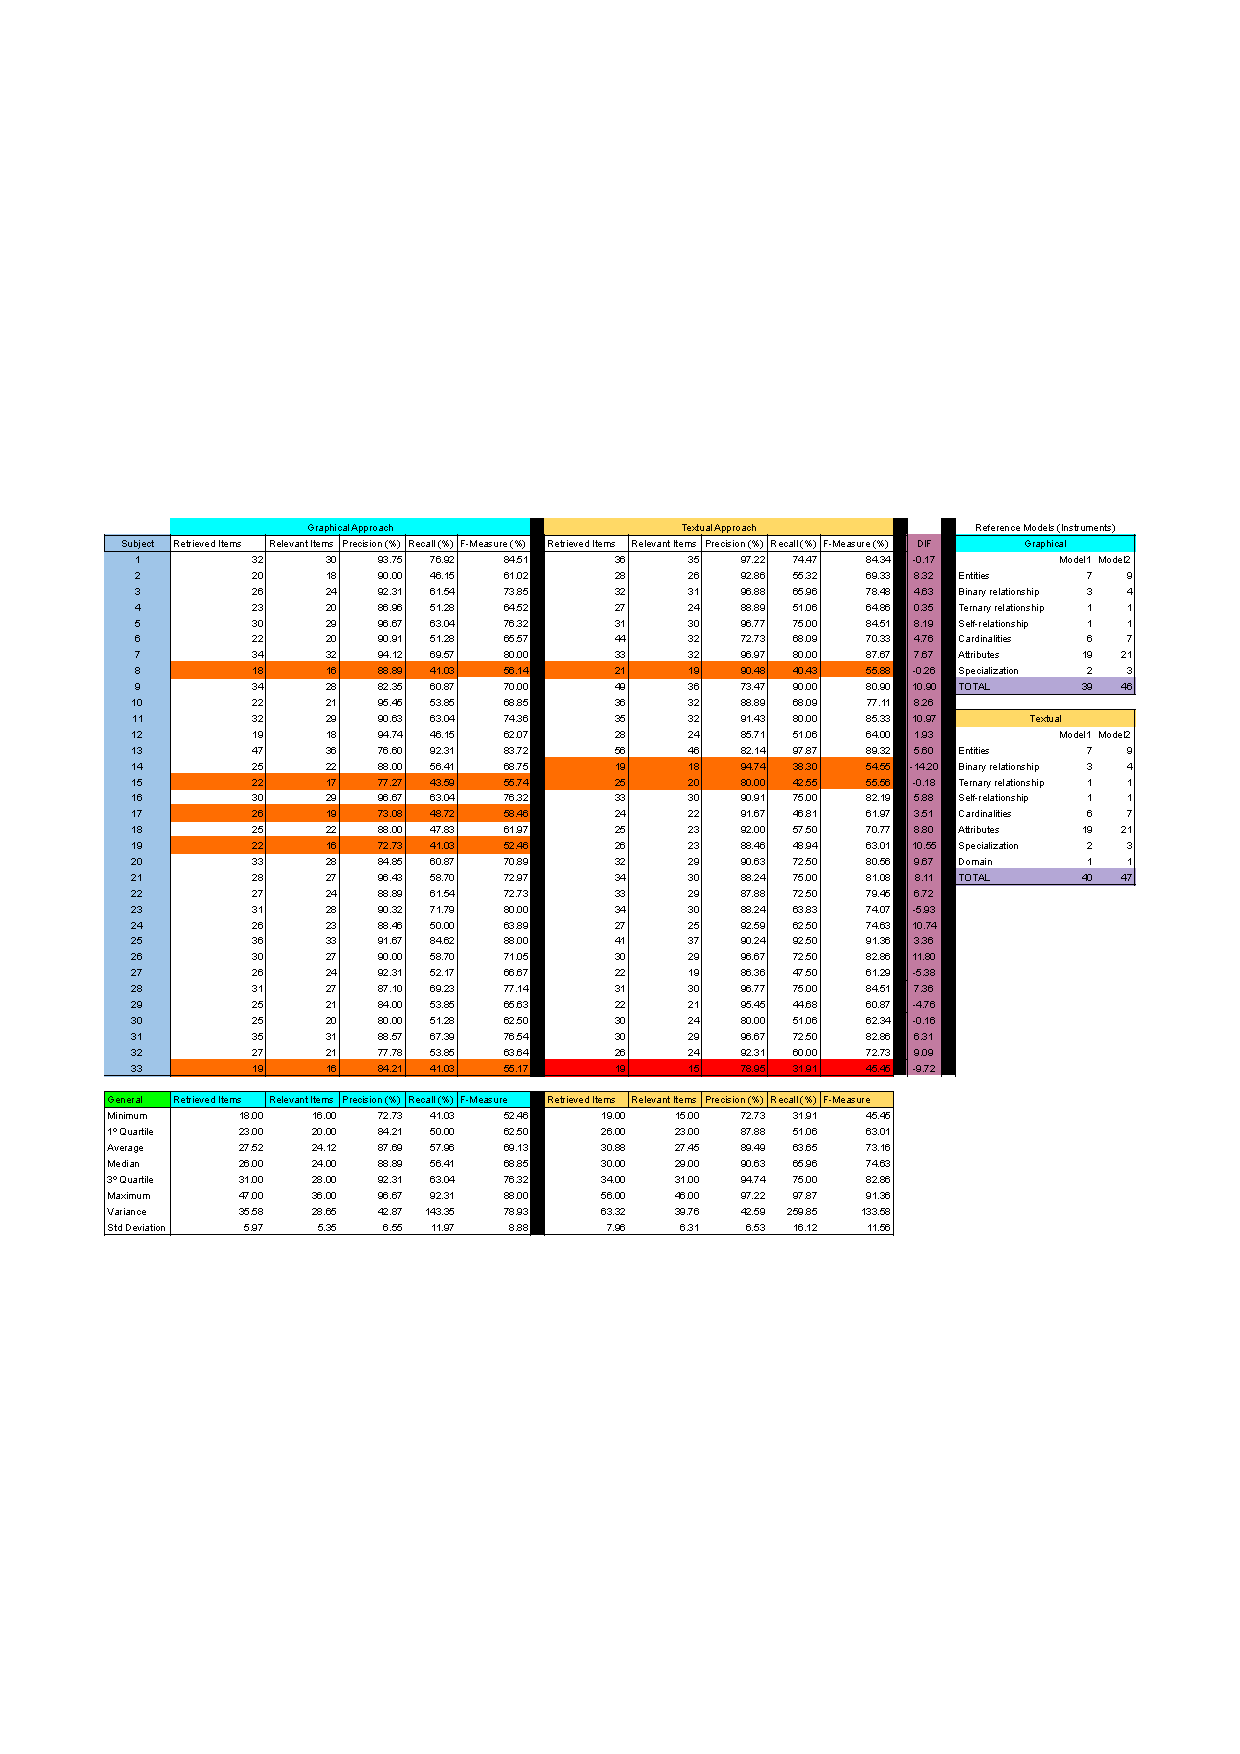
\includegraphics[]{postextuais/appendix/EX1-Results.pdf}
    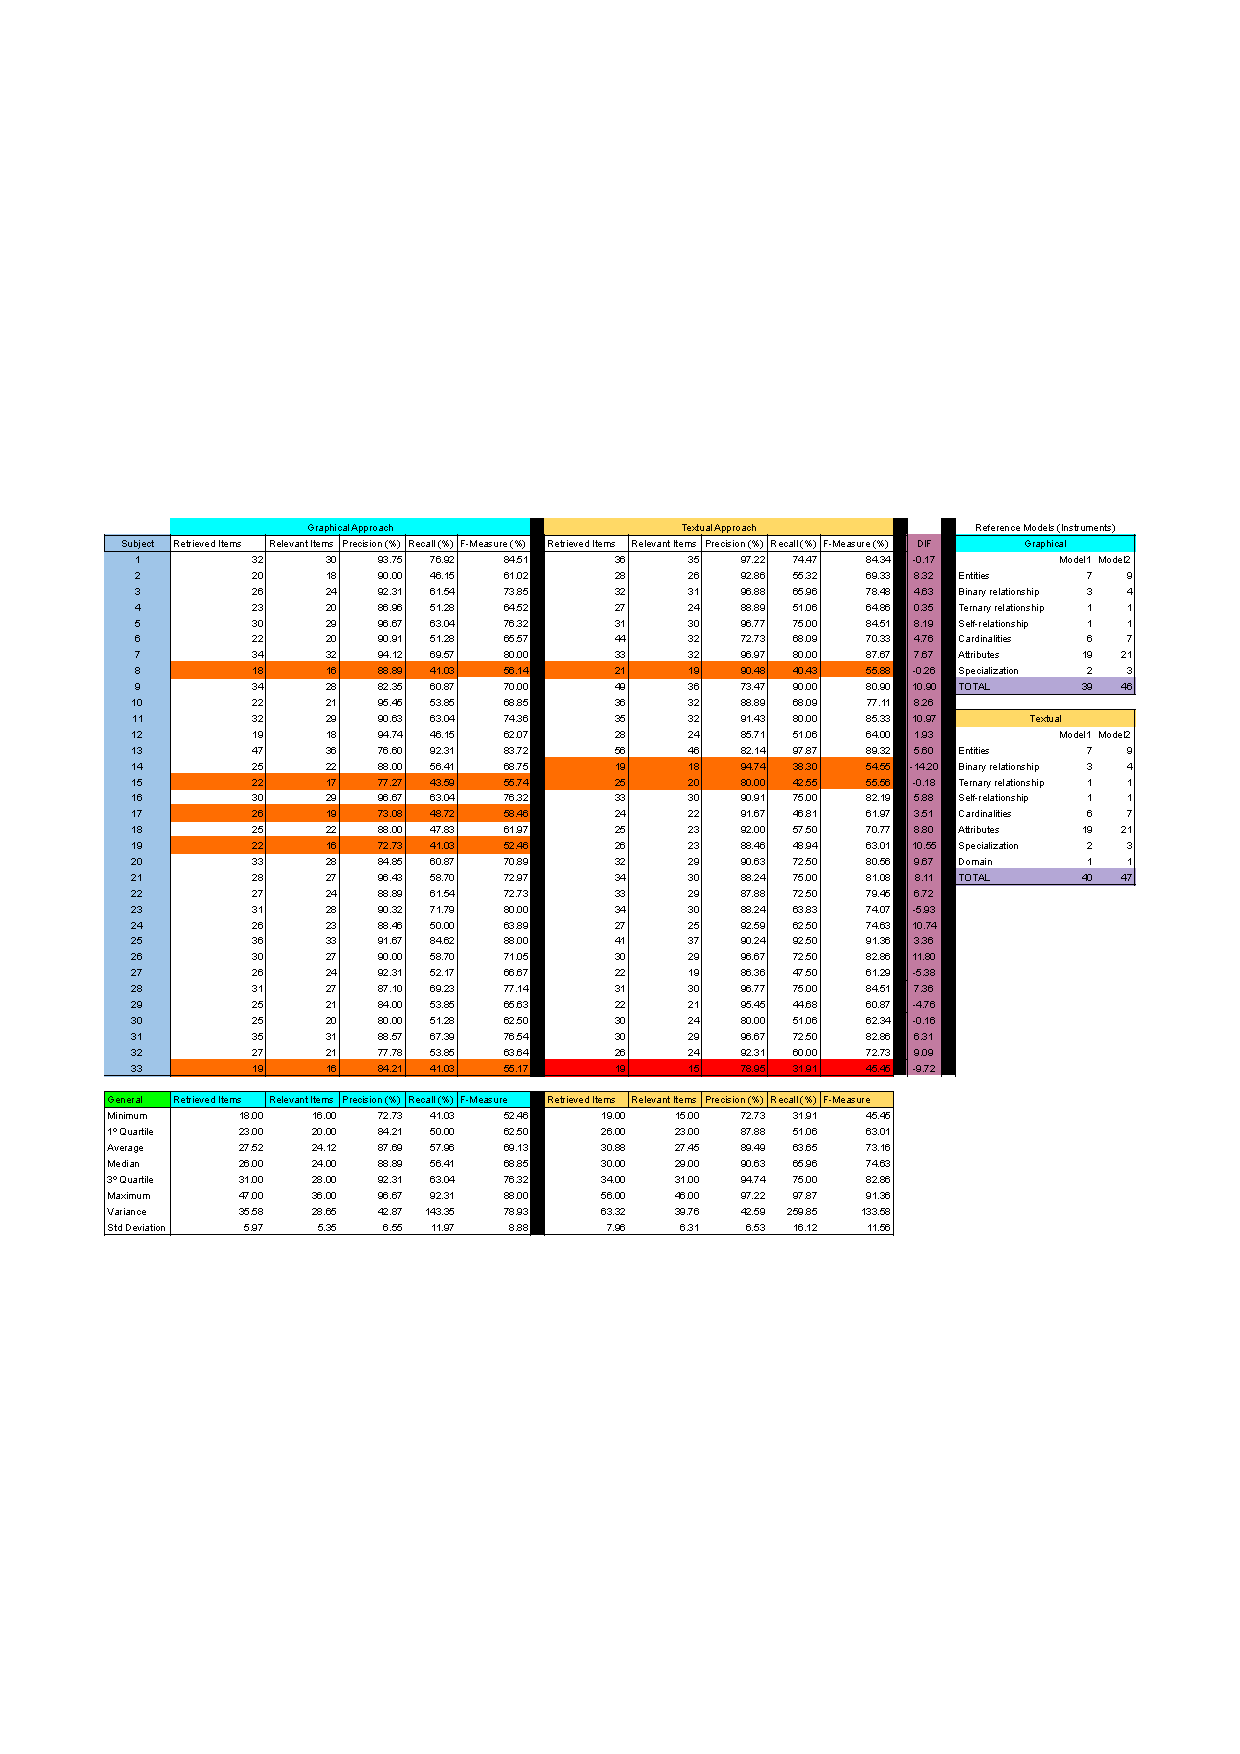
\includepdf[pages=-, frame=false, scale=0.90]{postextuais/appendix/EX1-Results.pdf}
    % \caption{EX1 - F-Score.}
    \label{fig:ex1FScore}
\end{figure}

\newpage

\section{Times - EX1}

\begin{figure}[!htb]
    \centering
    % 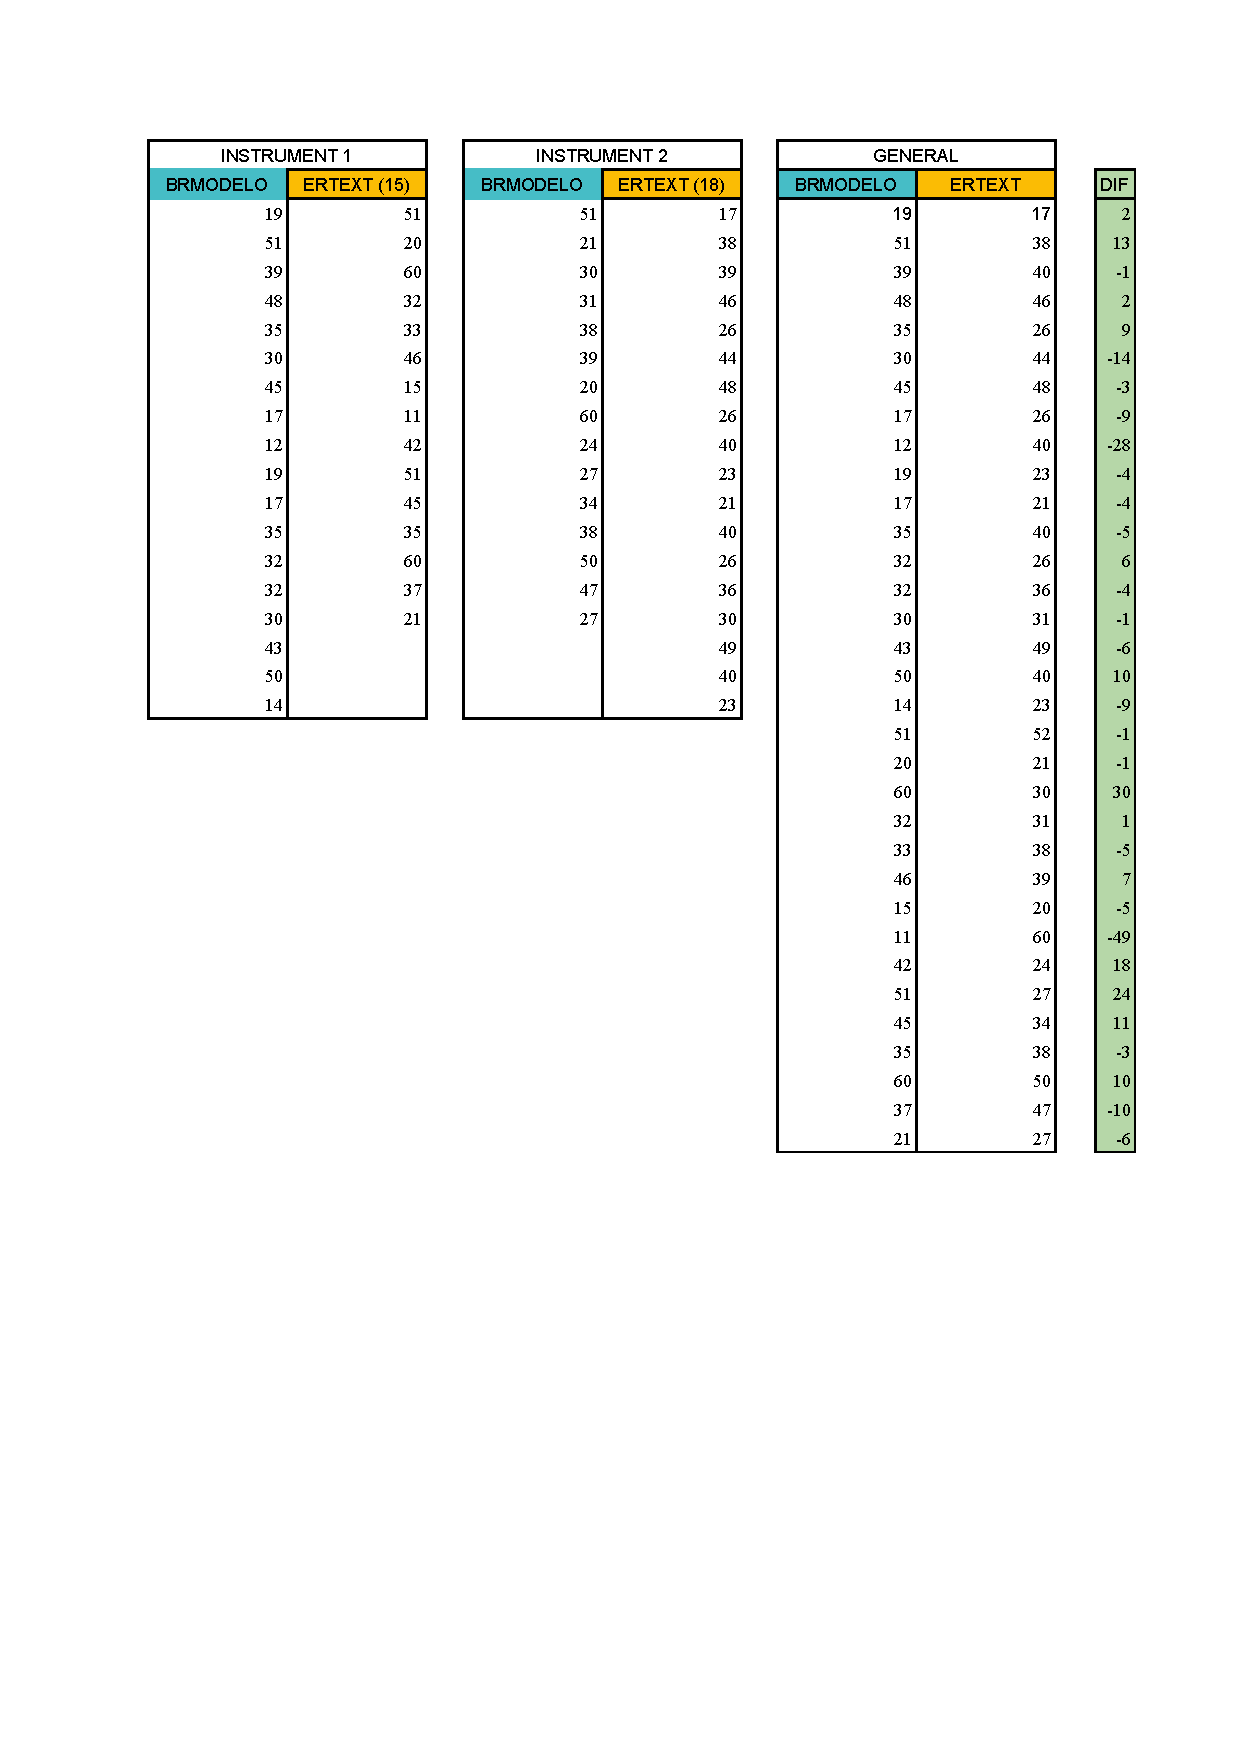
\includegraphics[]{postextuais/appendix/EX1-Results-Times.pdf}
    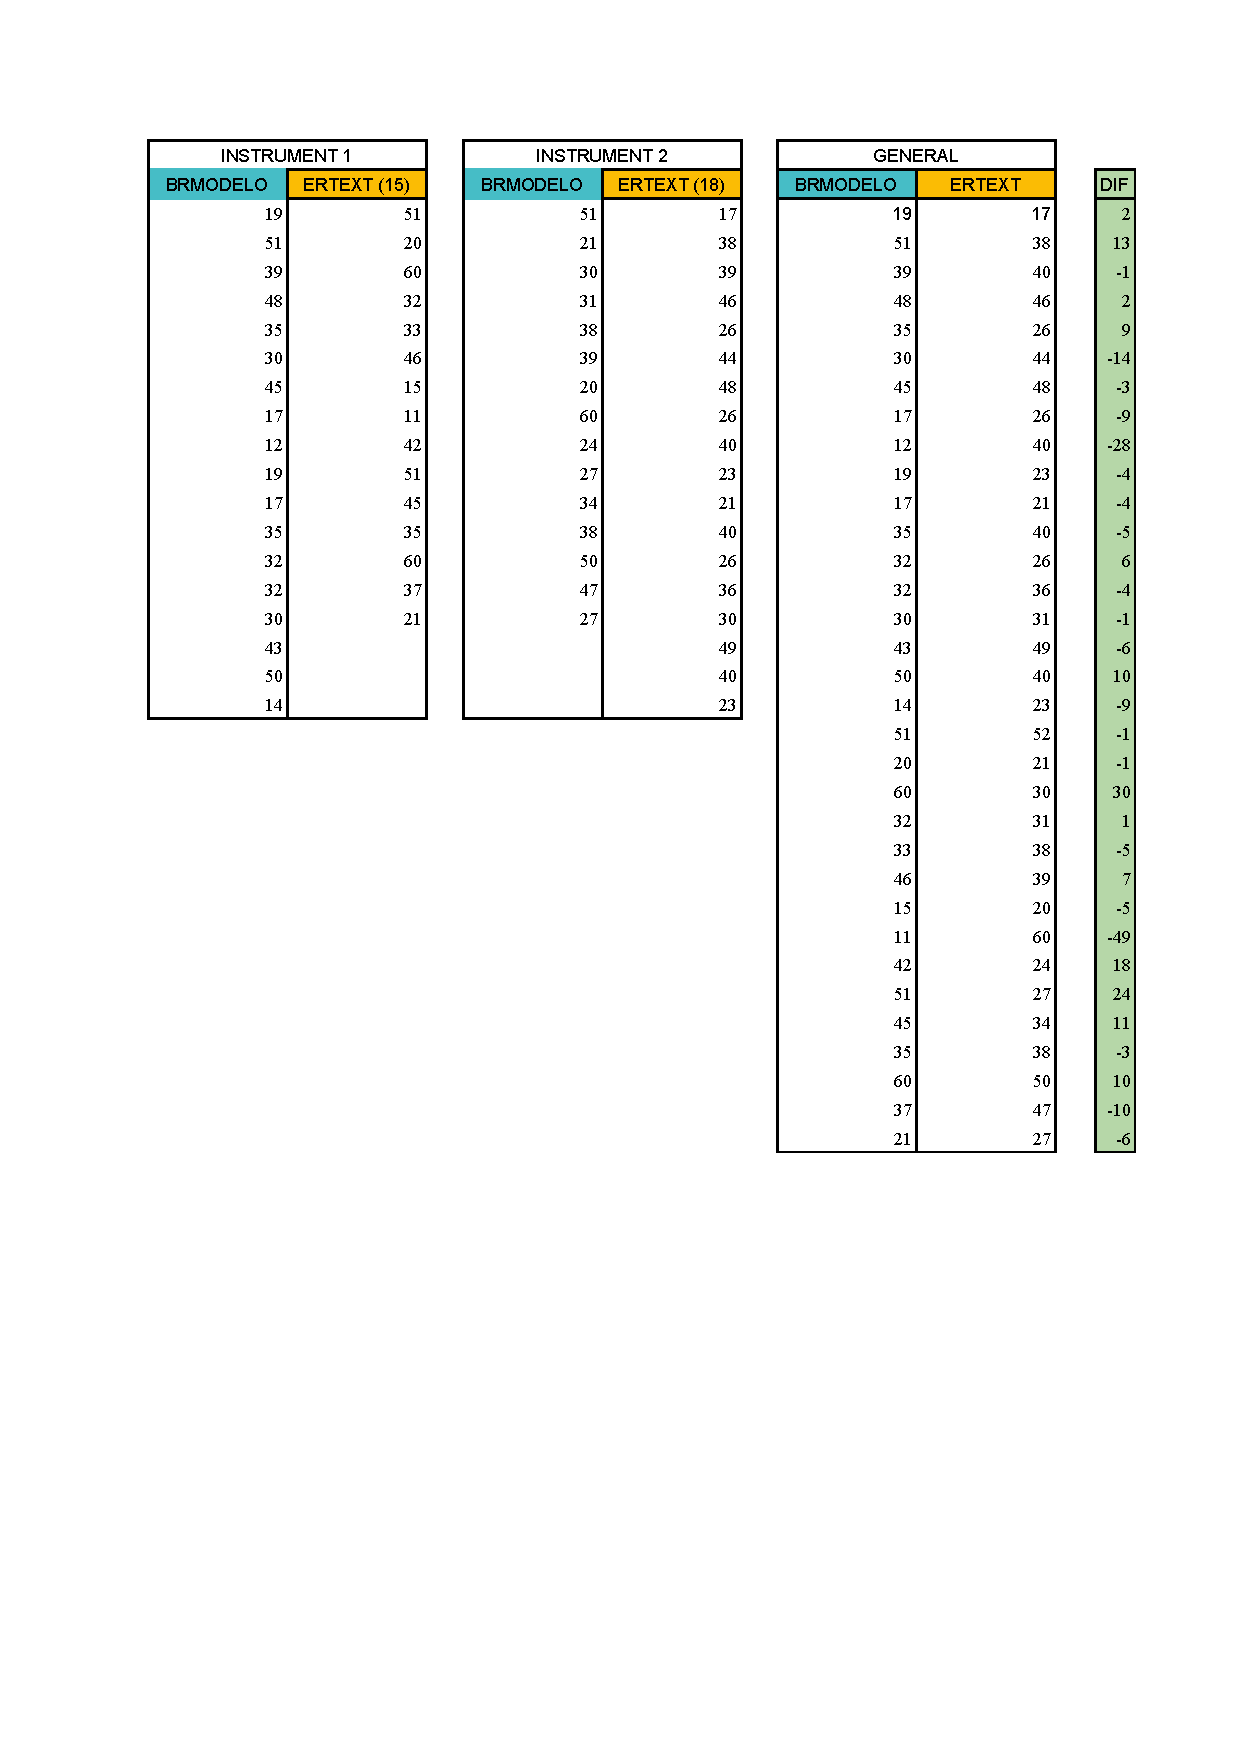
\includepdf[pages=-, frame=false, scale=0.80]{postextuais/appendix/EX1-Results-Times.pdf}
    % \caption{EX1 - times.}
    \label{fig:ex1Times}
\end{figure}

% ==============================================================================
\chapter{Experiment 2 (EX2)}
% ==============================================================================

\section{F-score - EX2}

\begin{figure}[!htb]
    \centering
    % 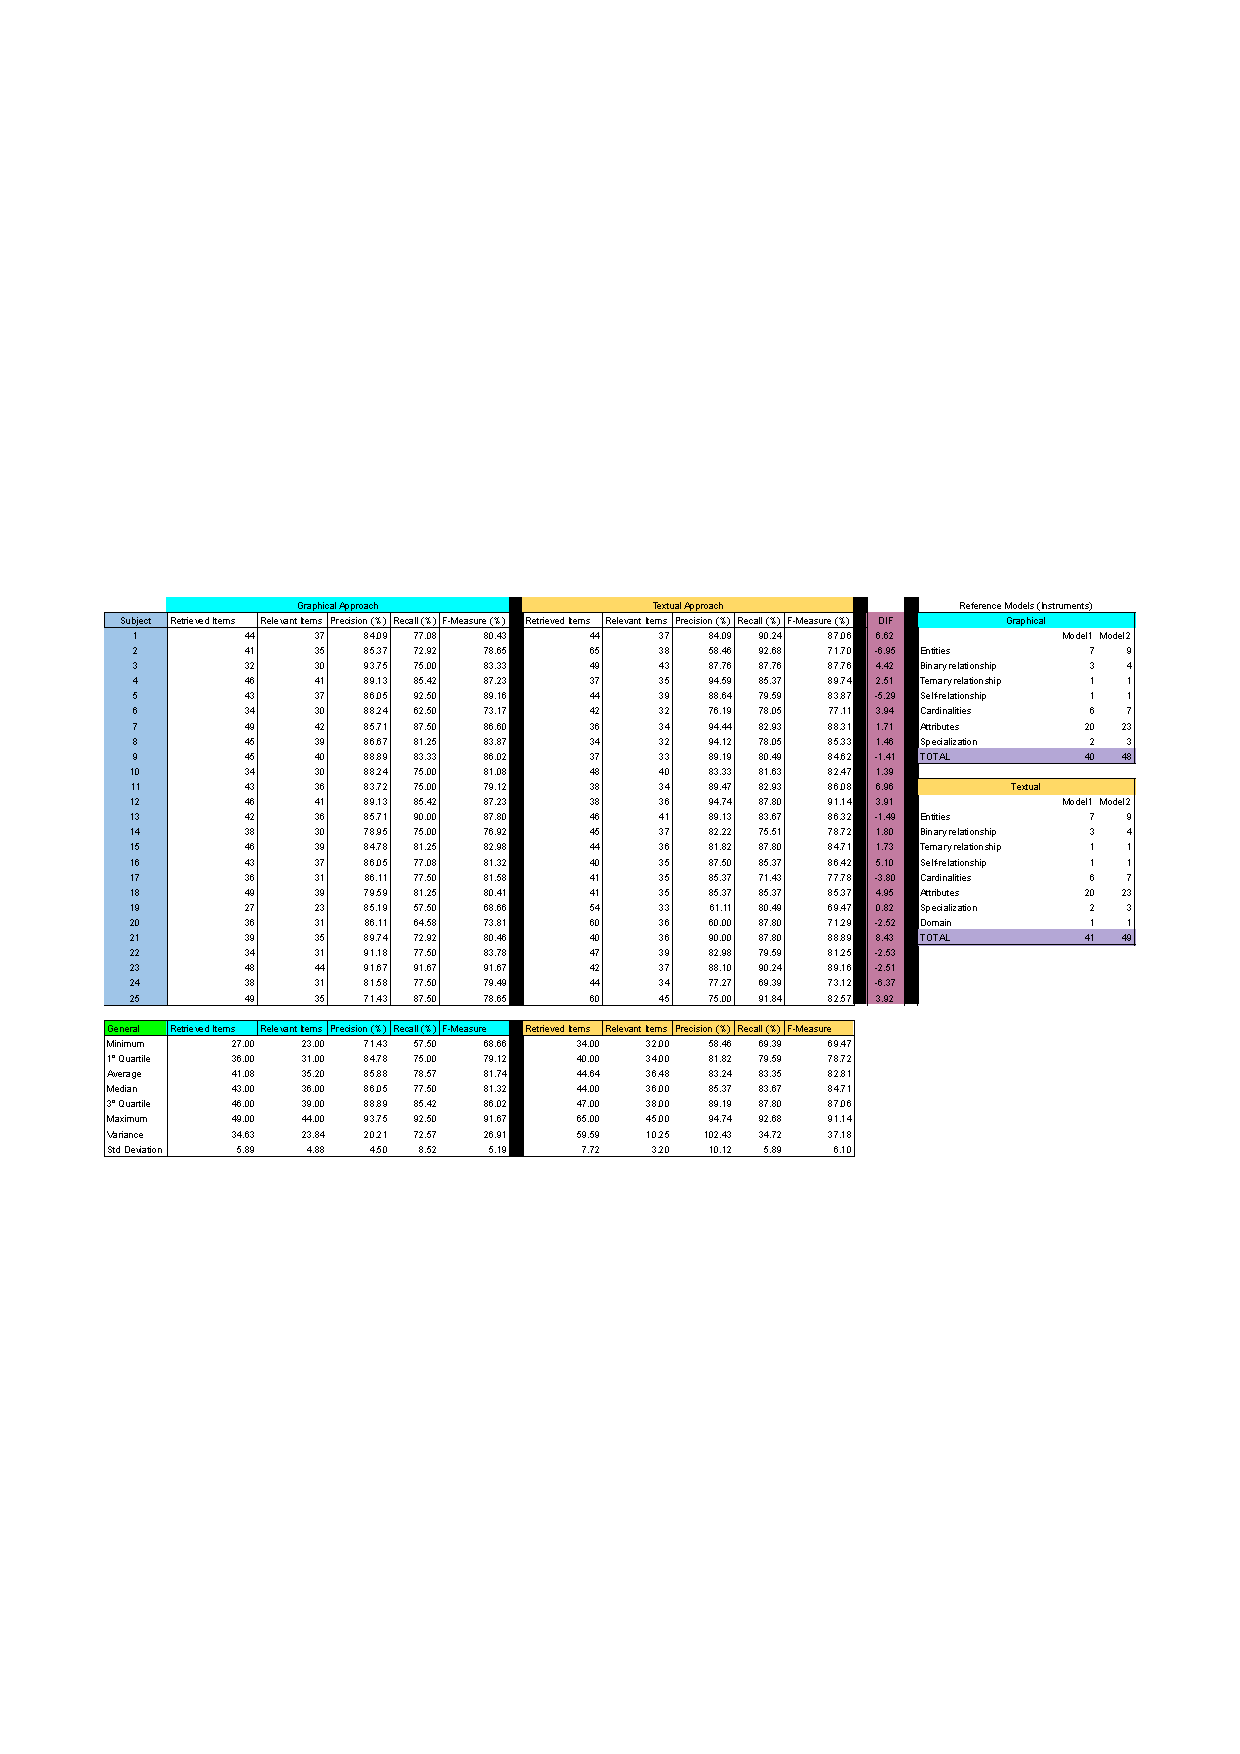
\includegraphics[]{postextuais/appendix/EX2-Results.pdf}
    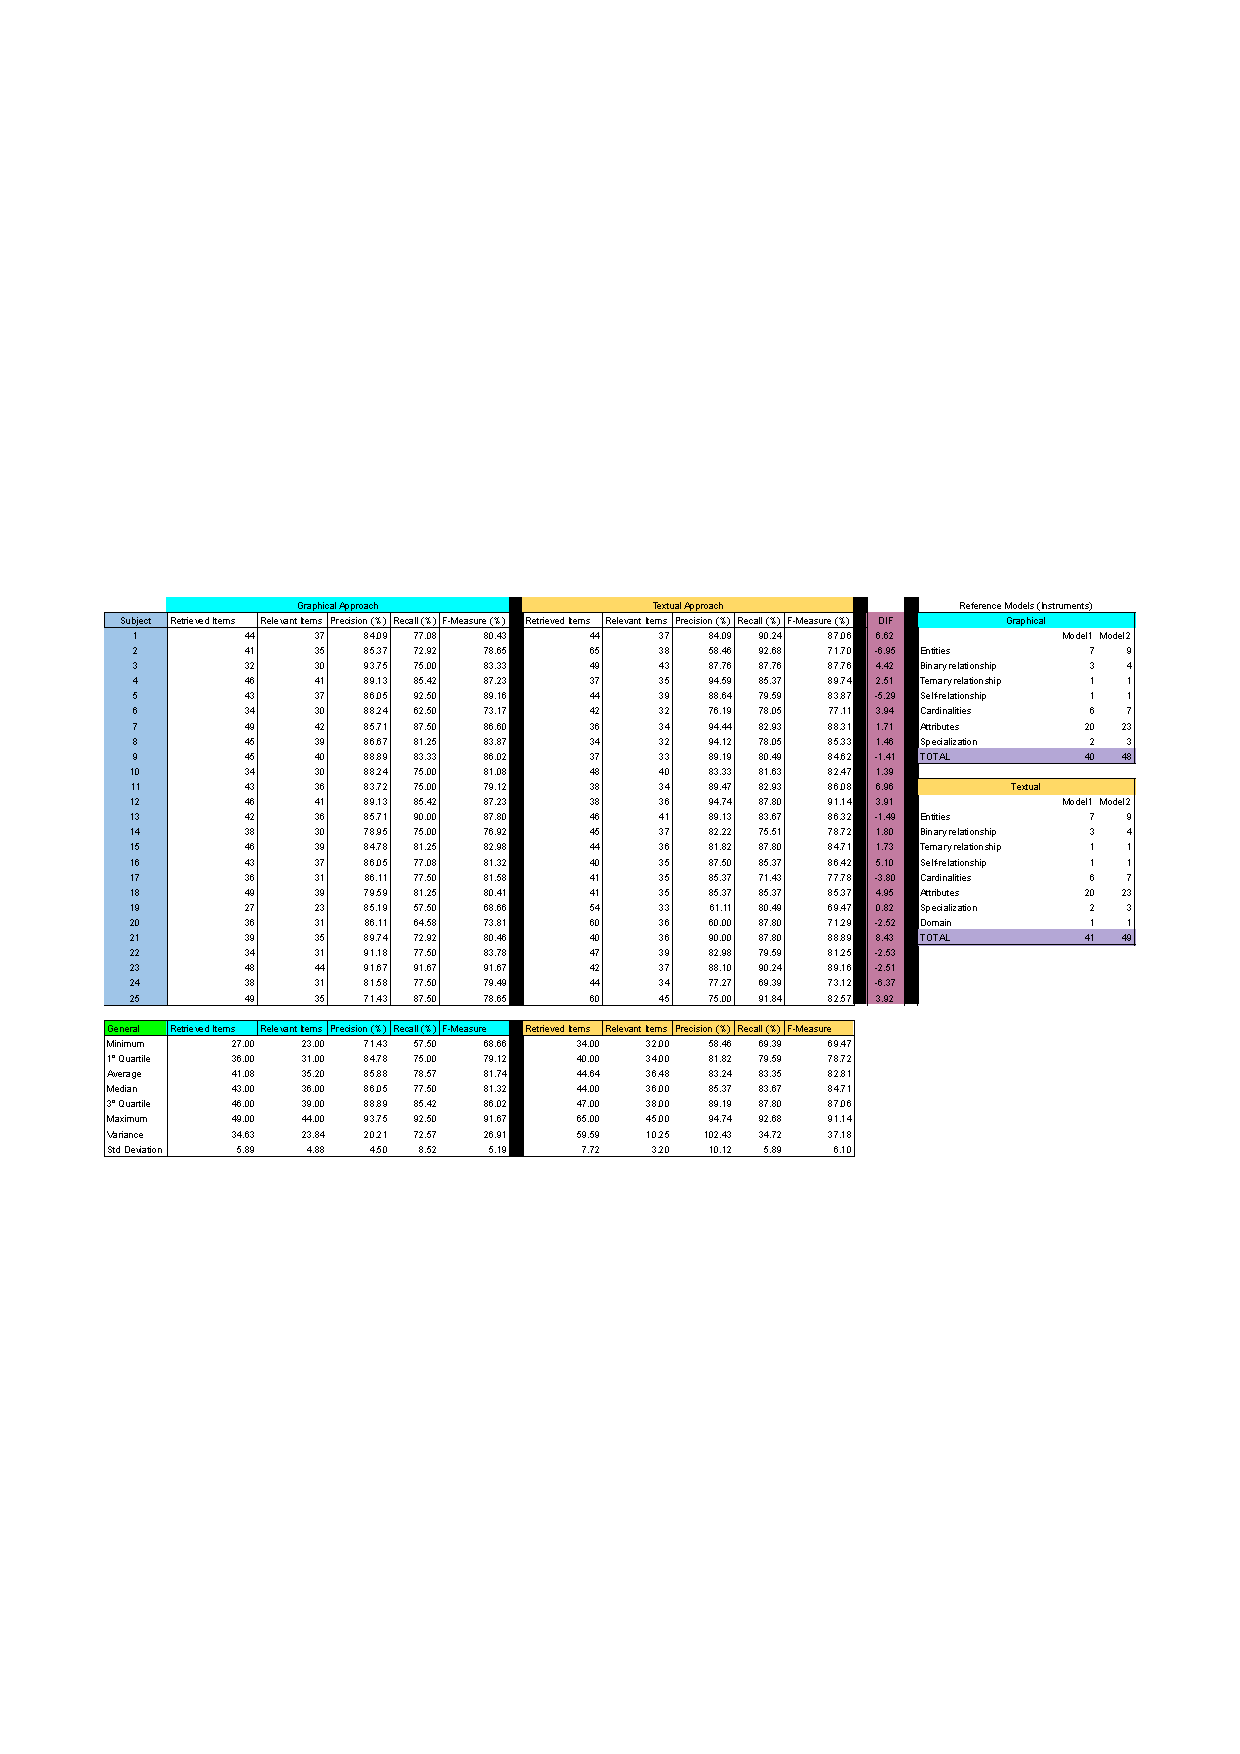
\includepdf[pages=-, frame=false, scale=0.90]{postextuais/appendix/EX2-Results.pdf}
    % \caption{EX2 - F-Score.}
    \label{fig:ex2FScore}
\end{figure}

\newpage

\section{Times - EX2}

\begin{figure}[!htb]
    \centering
    % 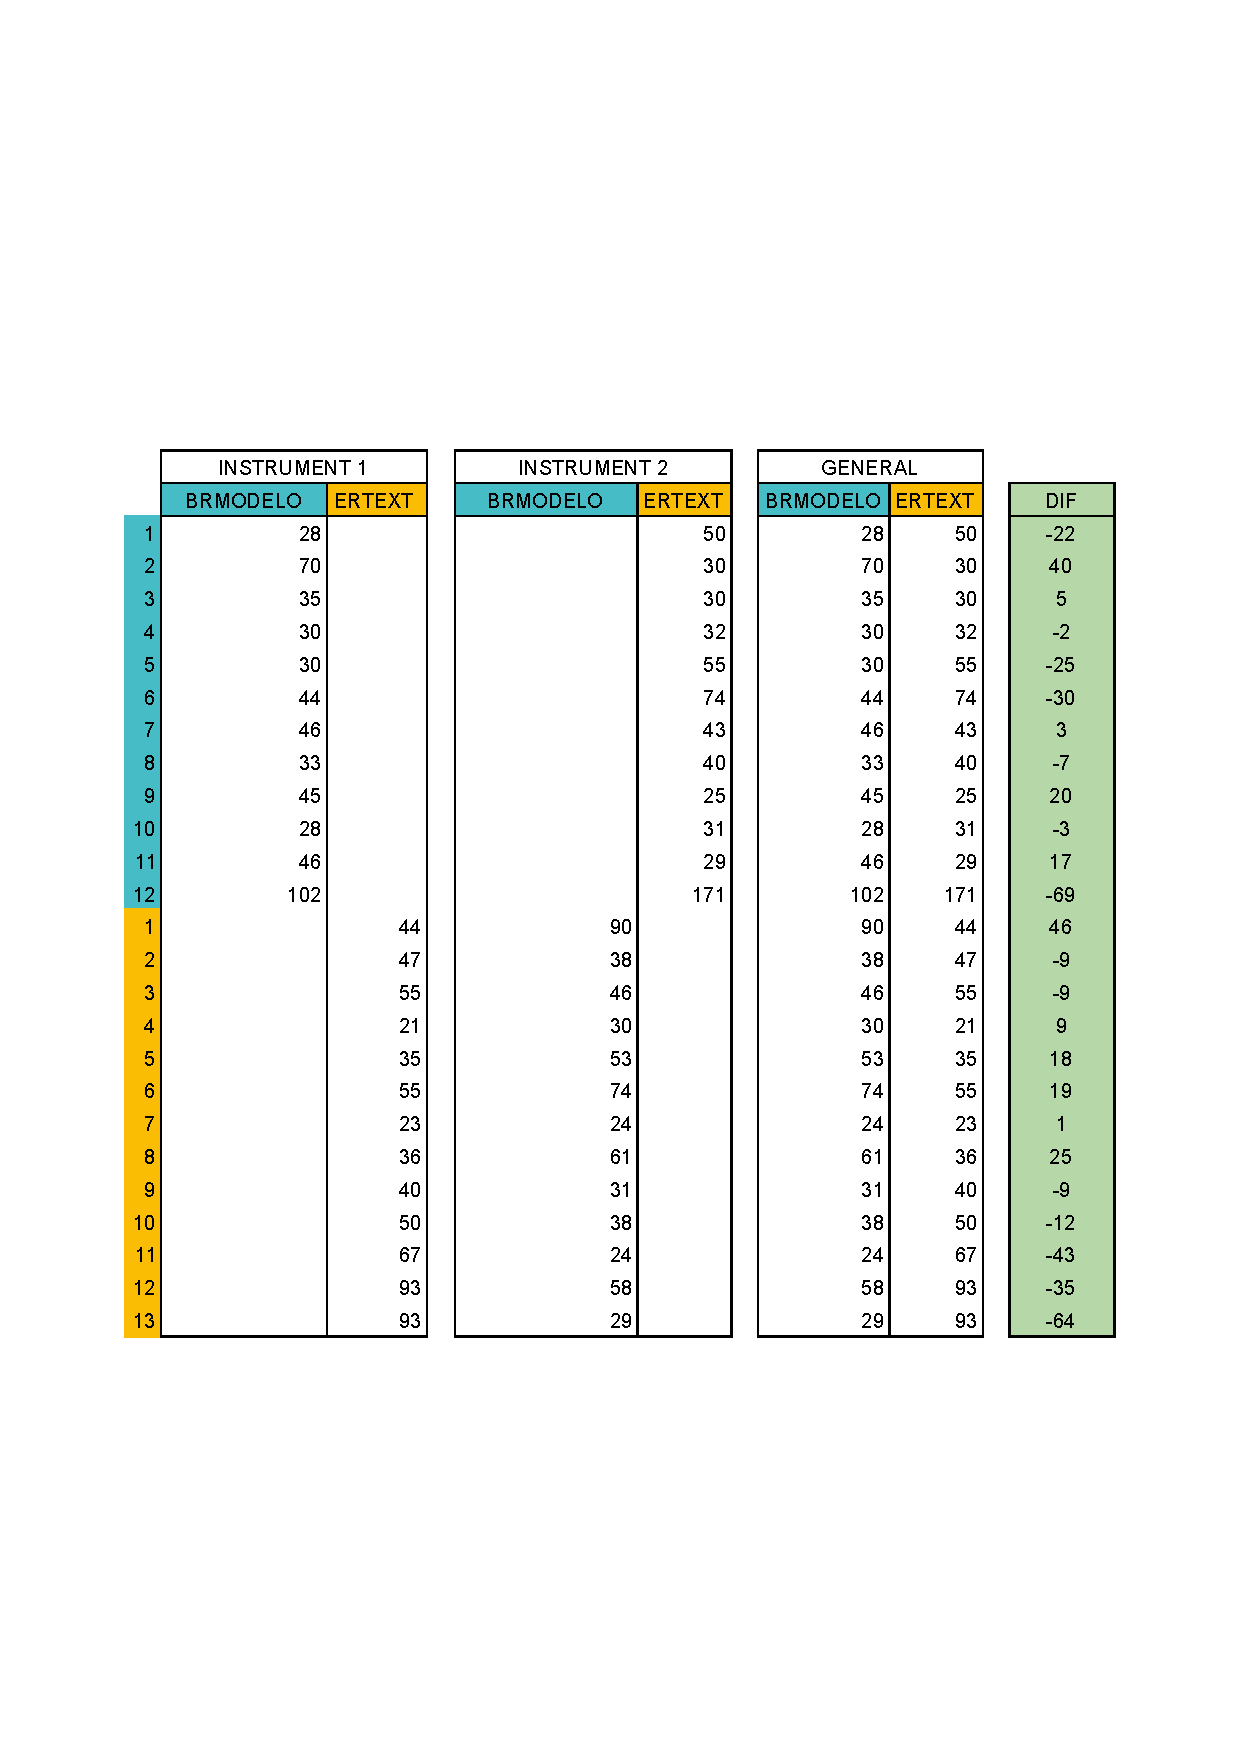
\includegraphics[]{postextuais/appendix/EX2-Results-Times.pdf}
    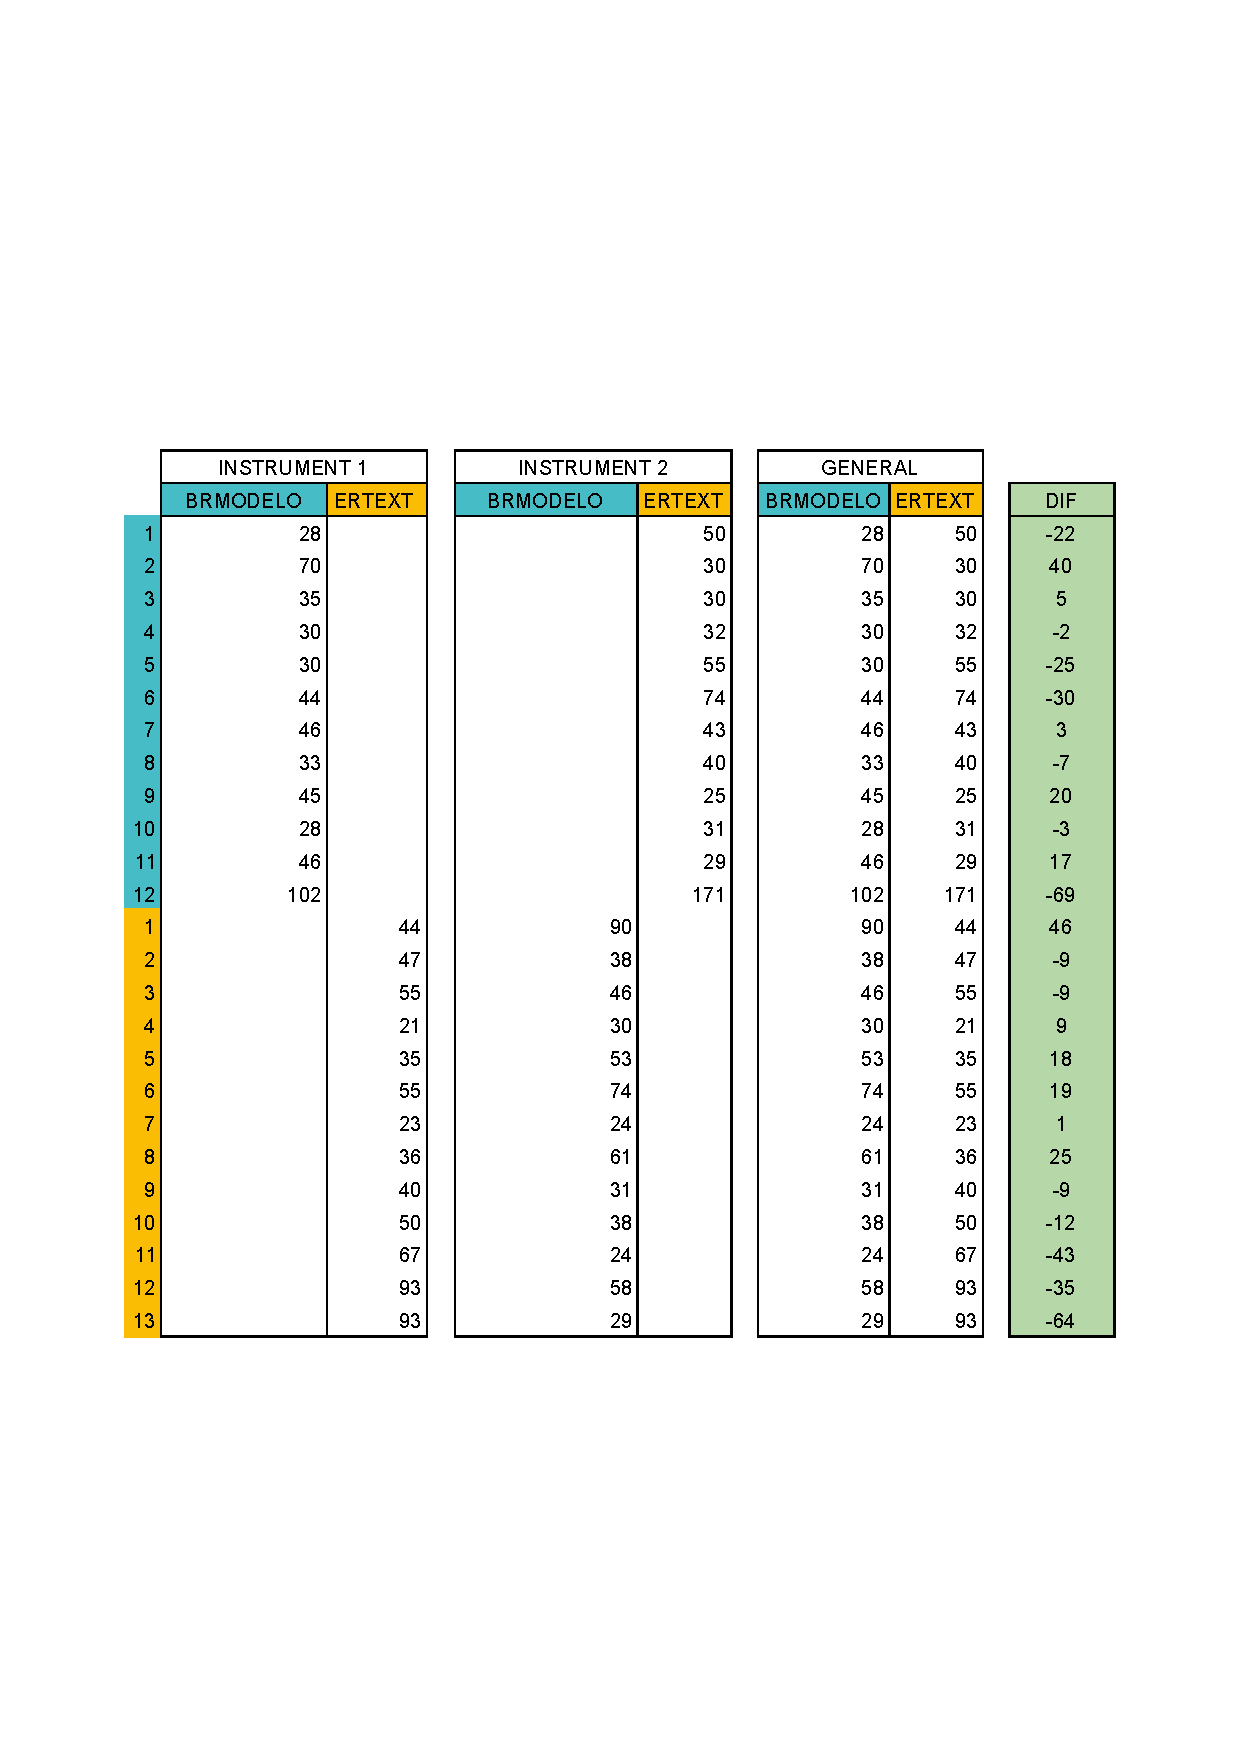
\includepdf[pages=-, frame=false, scale=0.90]{postextuais/appendix/EX2-Results-Times.pdf}
    % \caption{EX2 - Times.}
    \label{fig:ex2Times}
\end{figure}

\newpage

\section{Emocards - EX2}

\begin{figure}[!htb]
    \centering
    % 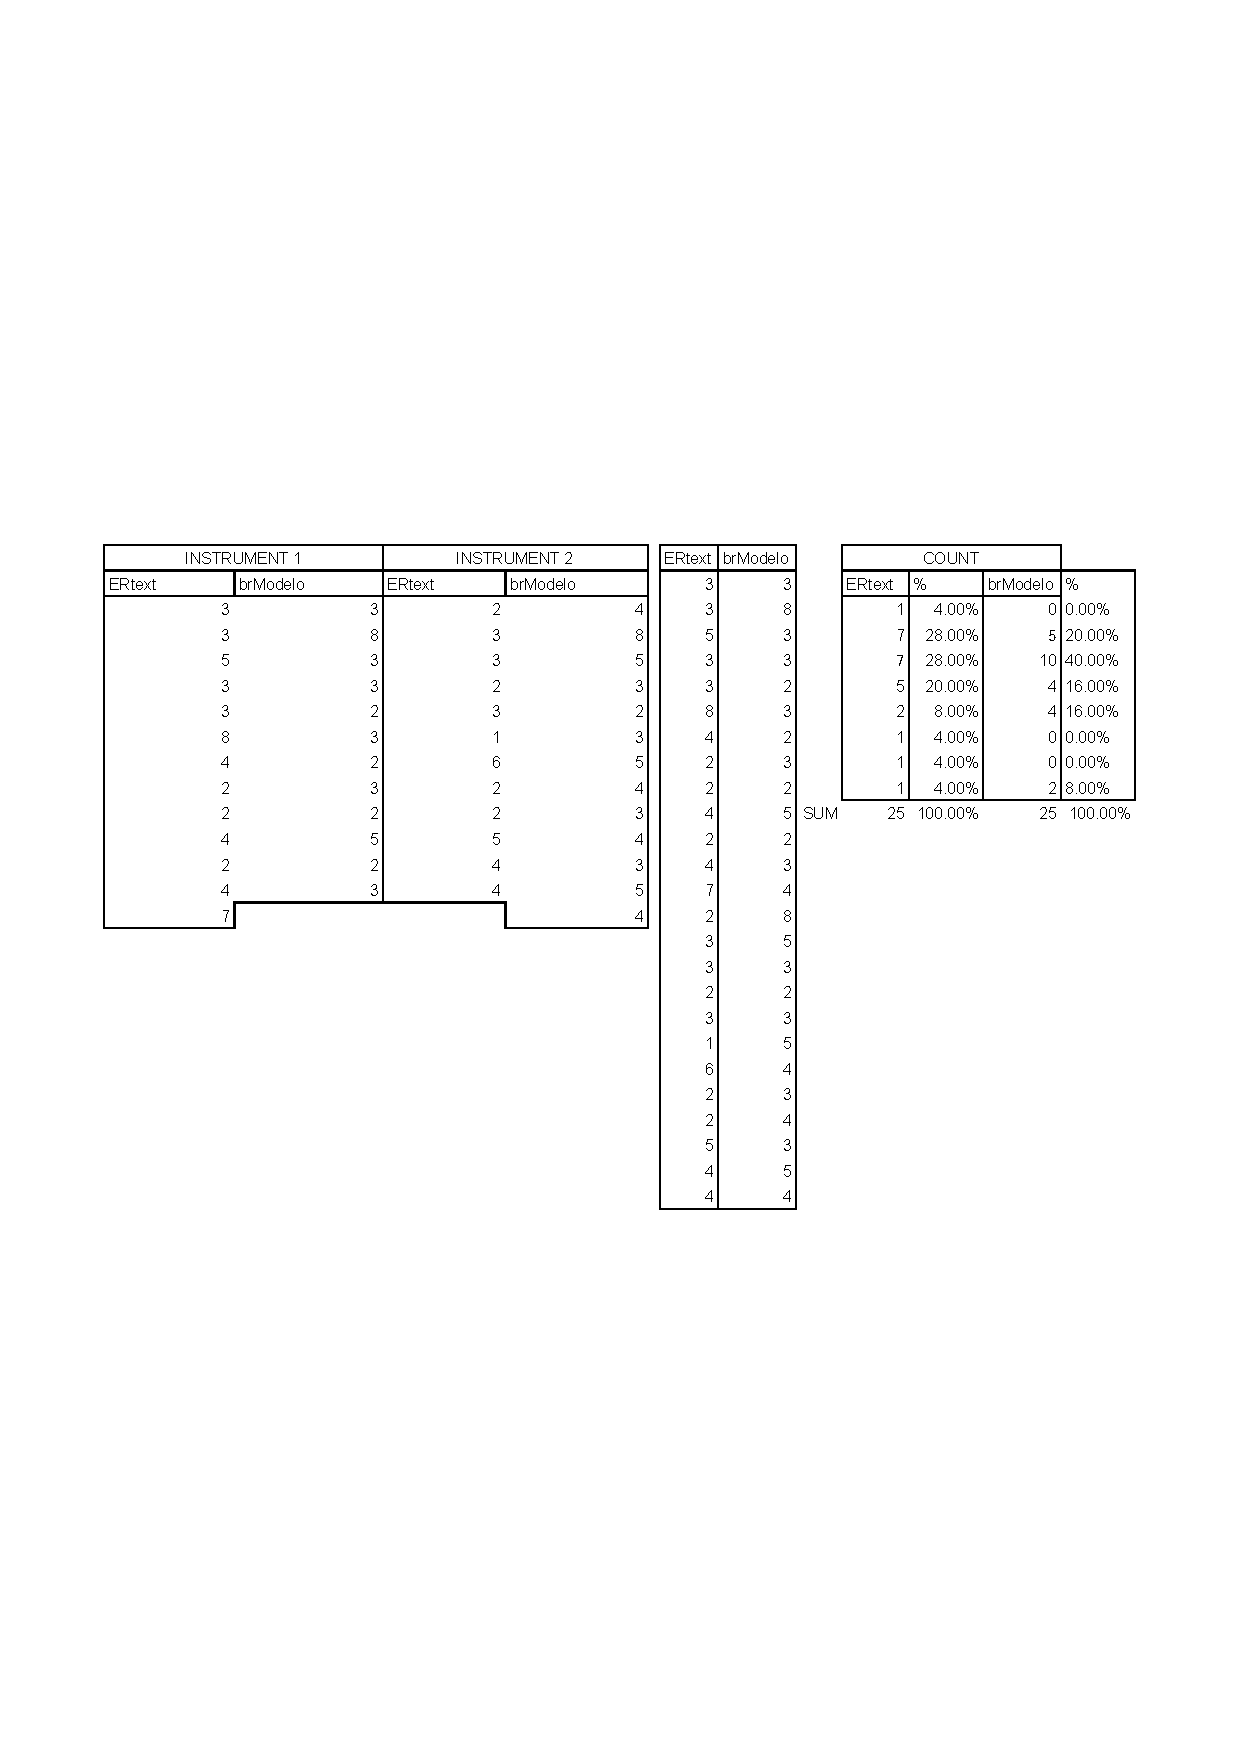
\includegraphics[]{postextuais/appendix/EX2-Results-Emocards.pdf}
    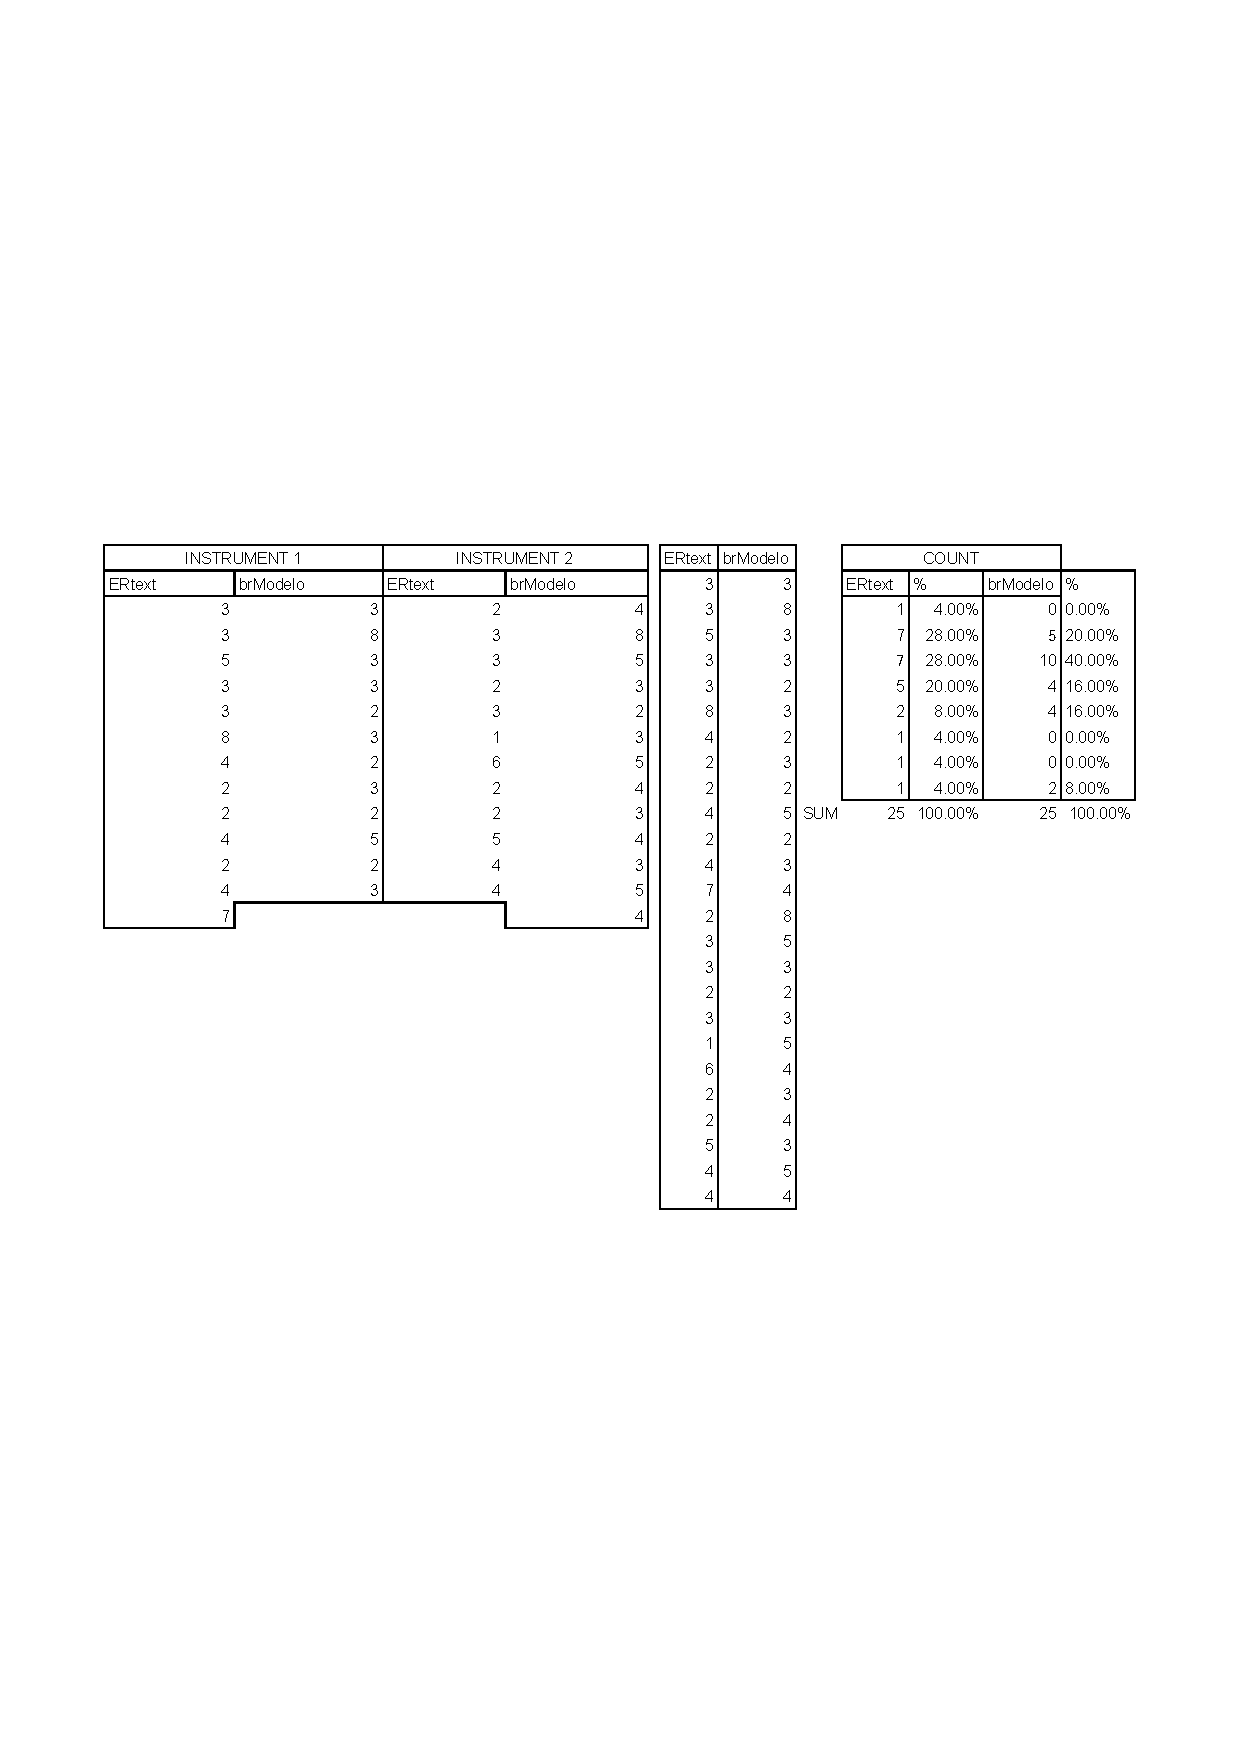
\includepdf[pages=-, frame=false, scale=0.90]{postextuais/appendix/EX2-Results-Emocards.pdf}
    % \caption{EX2 - Emocards.}
    \label{fig:ex2Emocards}
\end{figure}



% ==============================================================================
\chapter{Experiment 3 (EX3)}
% ==============================================================================

\section{Emocards - brModelo - EX3}

\begin{figure}[!htb]
    \centering
    % 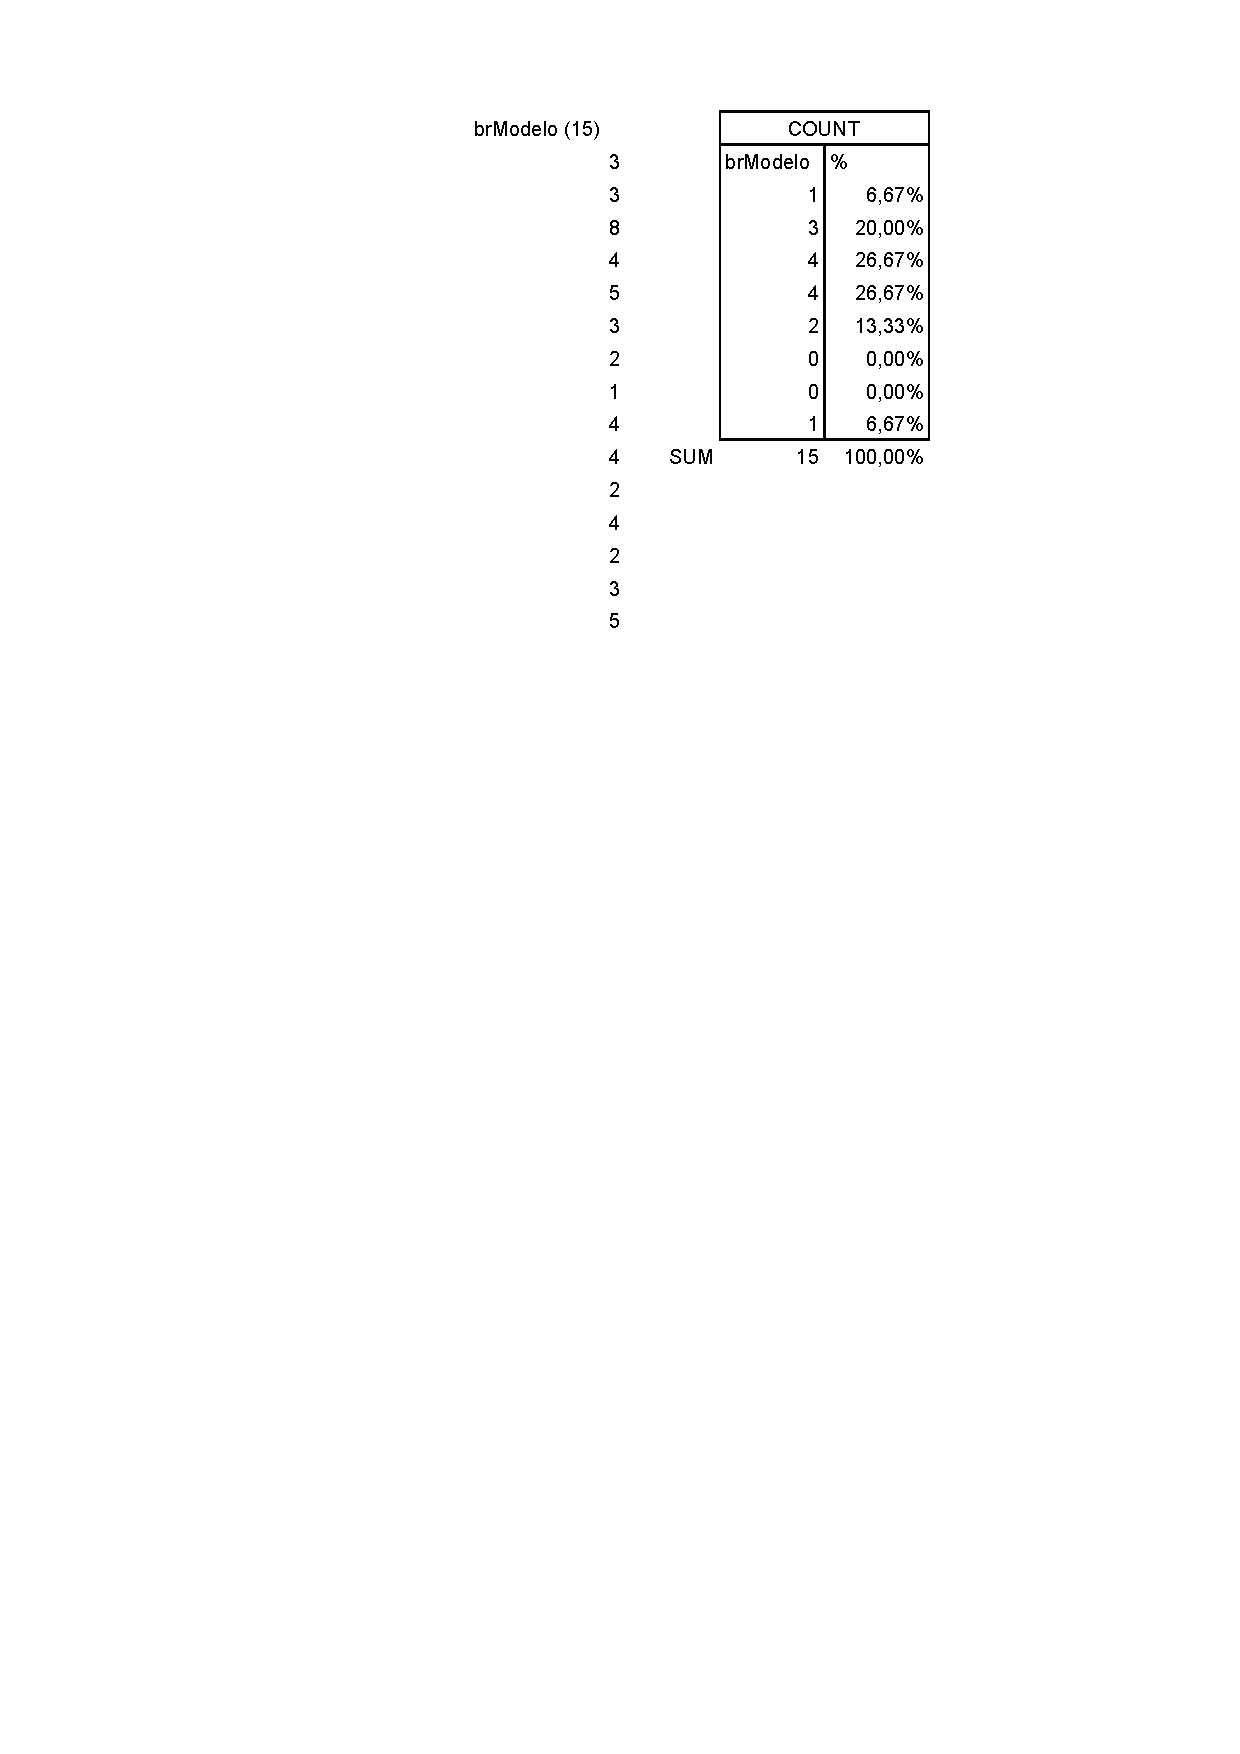
\includegraphics[]{postextuais/appendix/EX3- Emocards-brModelo.pdf}
    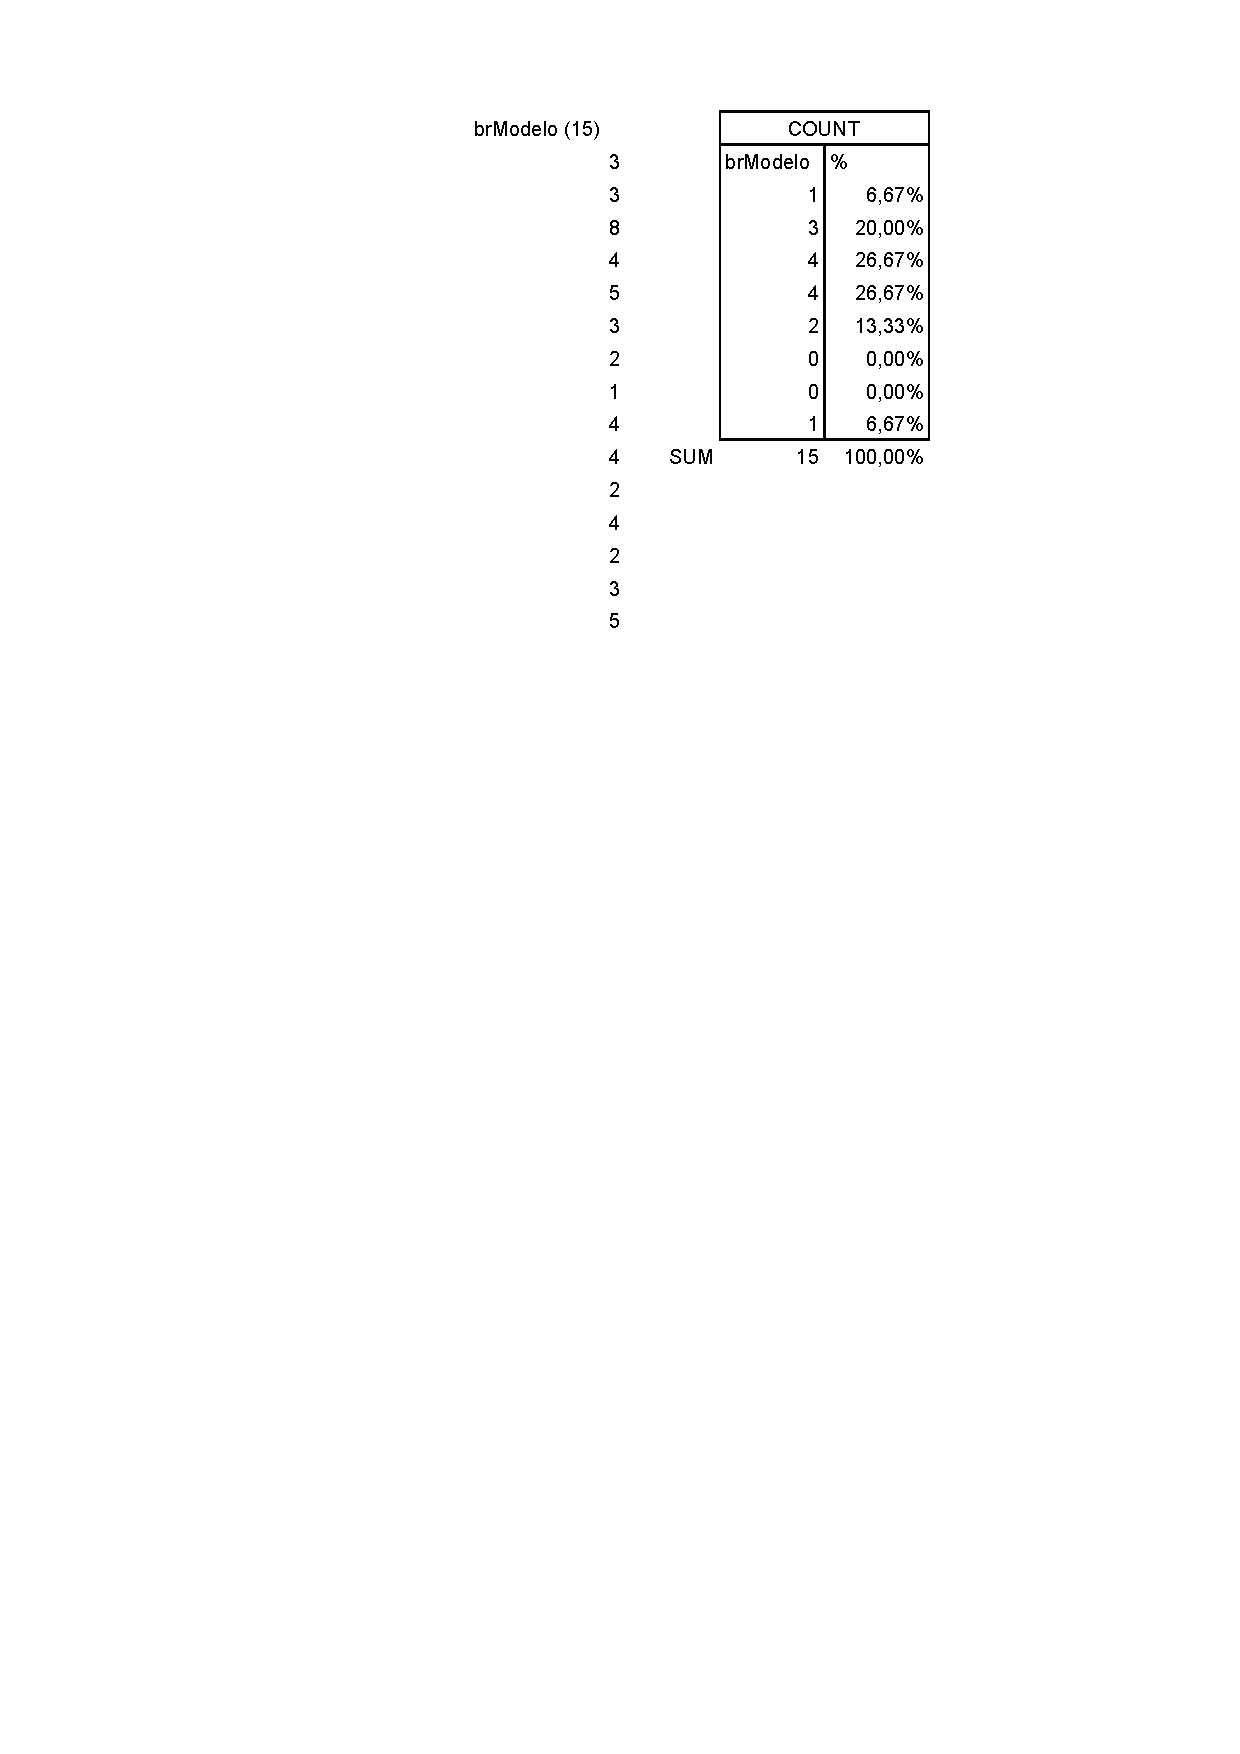
\includepdf[pages=-, frame=false, scale=0.70]{postextuais/appendix/EX3- Emocards-brModelo.pdf}
    % \caption{EX3 - Emocards - brModelo.}
    \label{fig:ex3EmocardsbrModelo}
\end{figure}

\newpage

\section{Emocards - ERtext - EX3}


\begin{figure}[!htb]
    \centering
    % 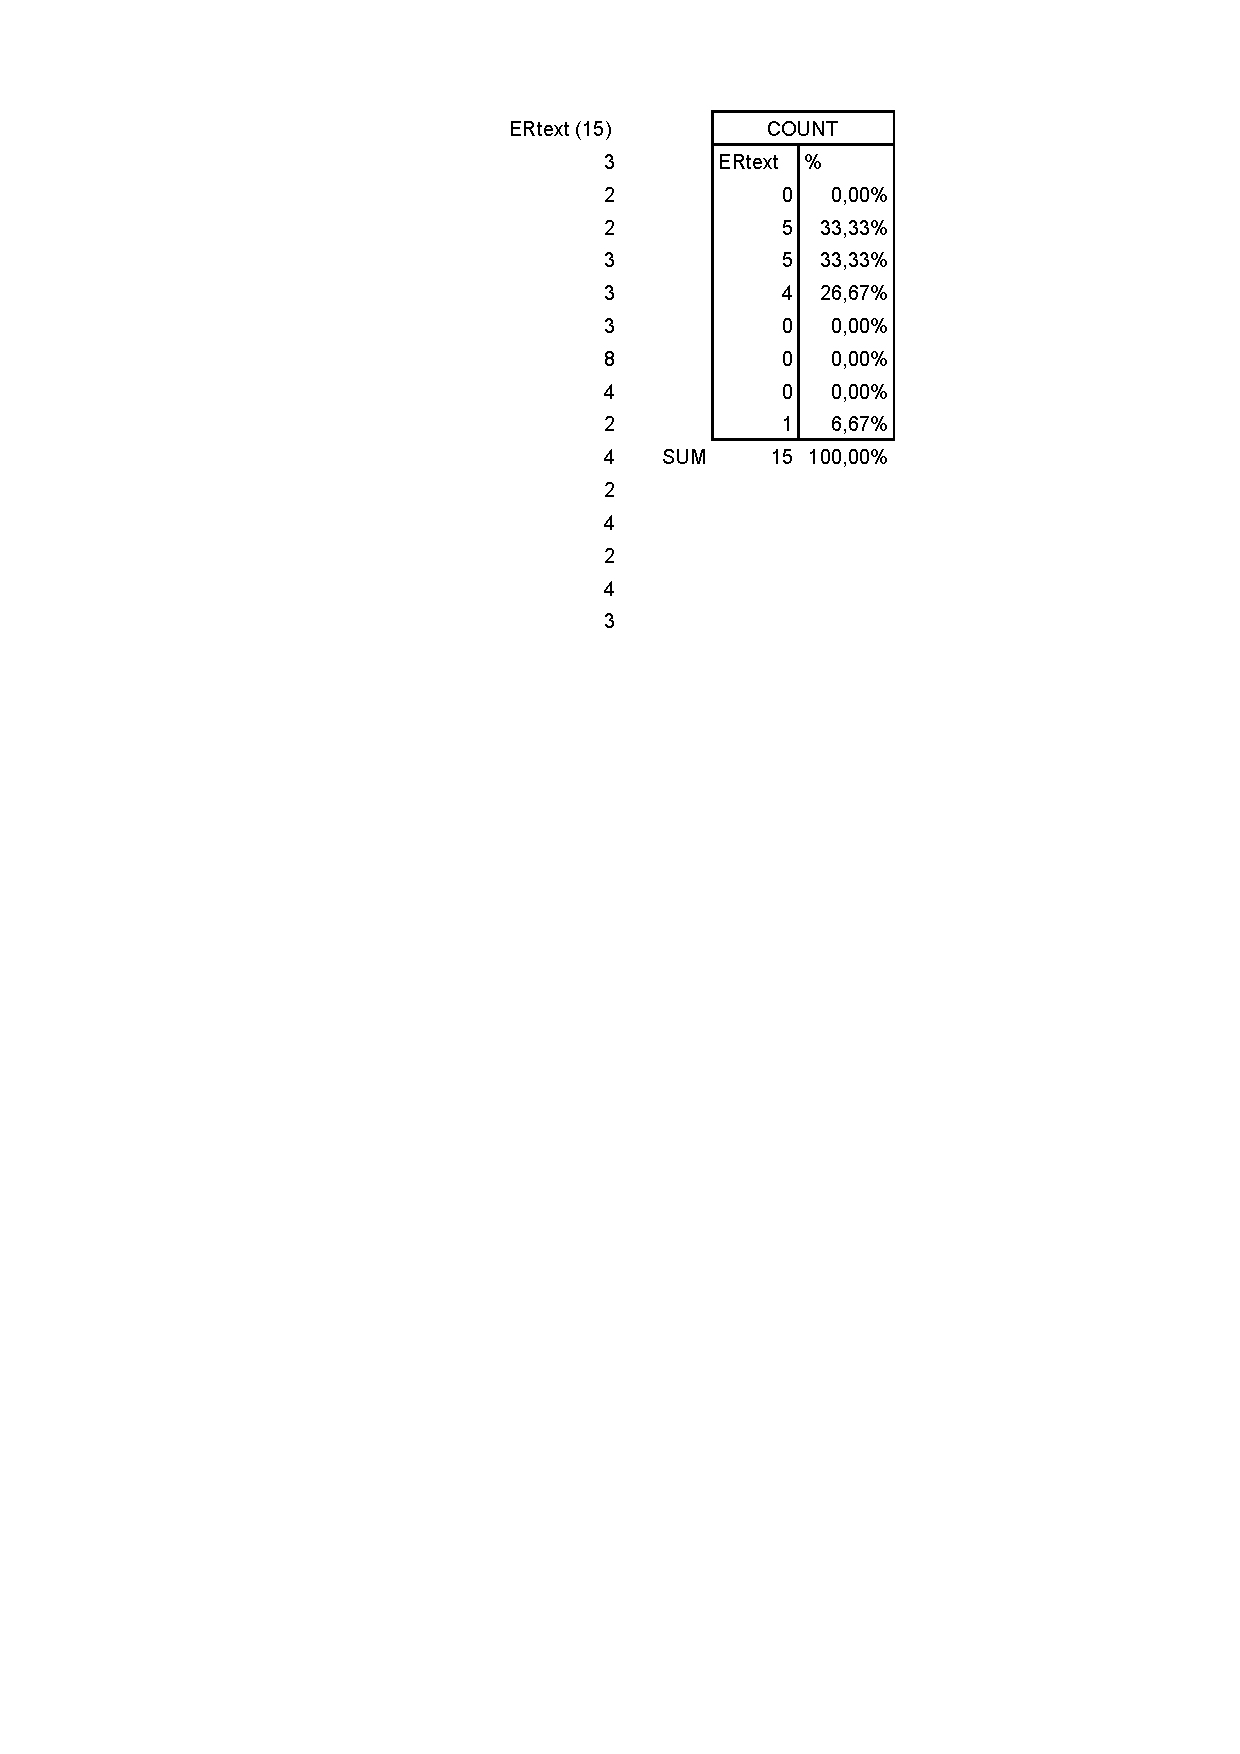
\includegraphics[]{postextuais/appendix/EX3- Emocards-ERtext.pdf}
    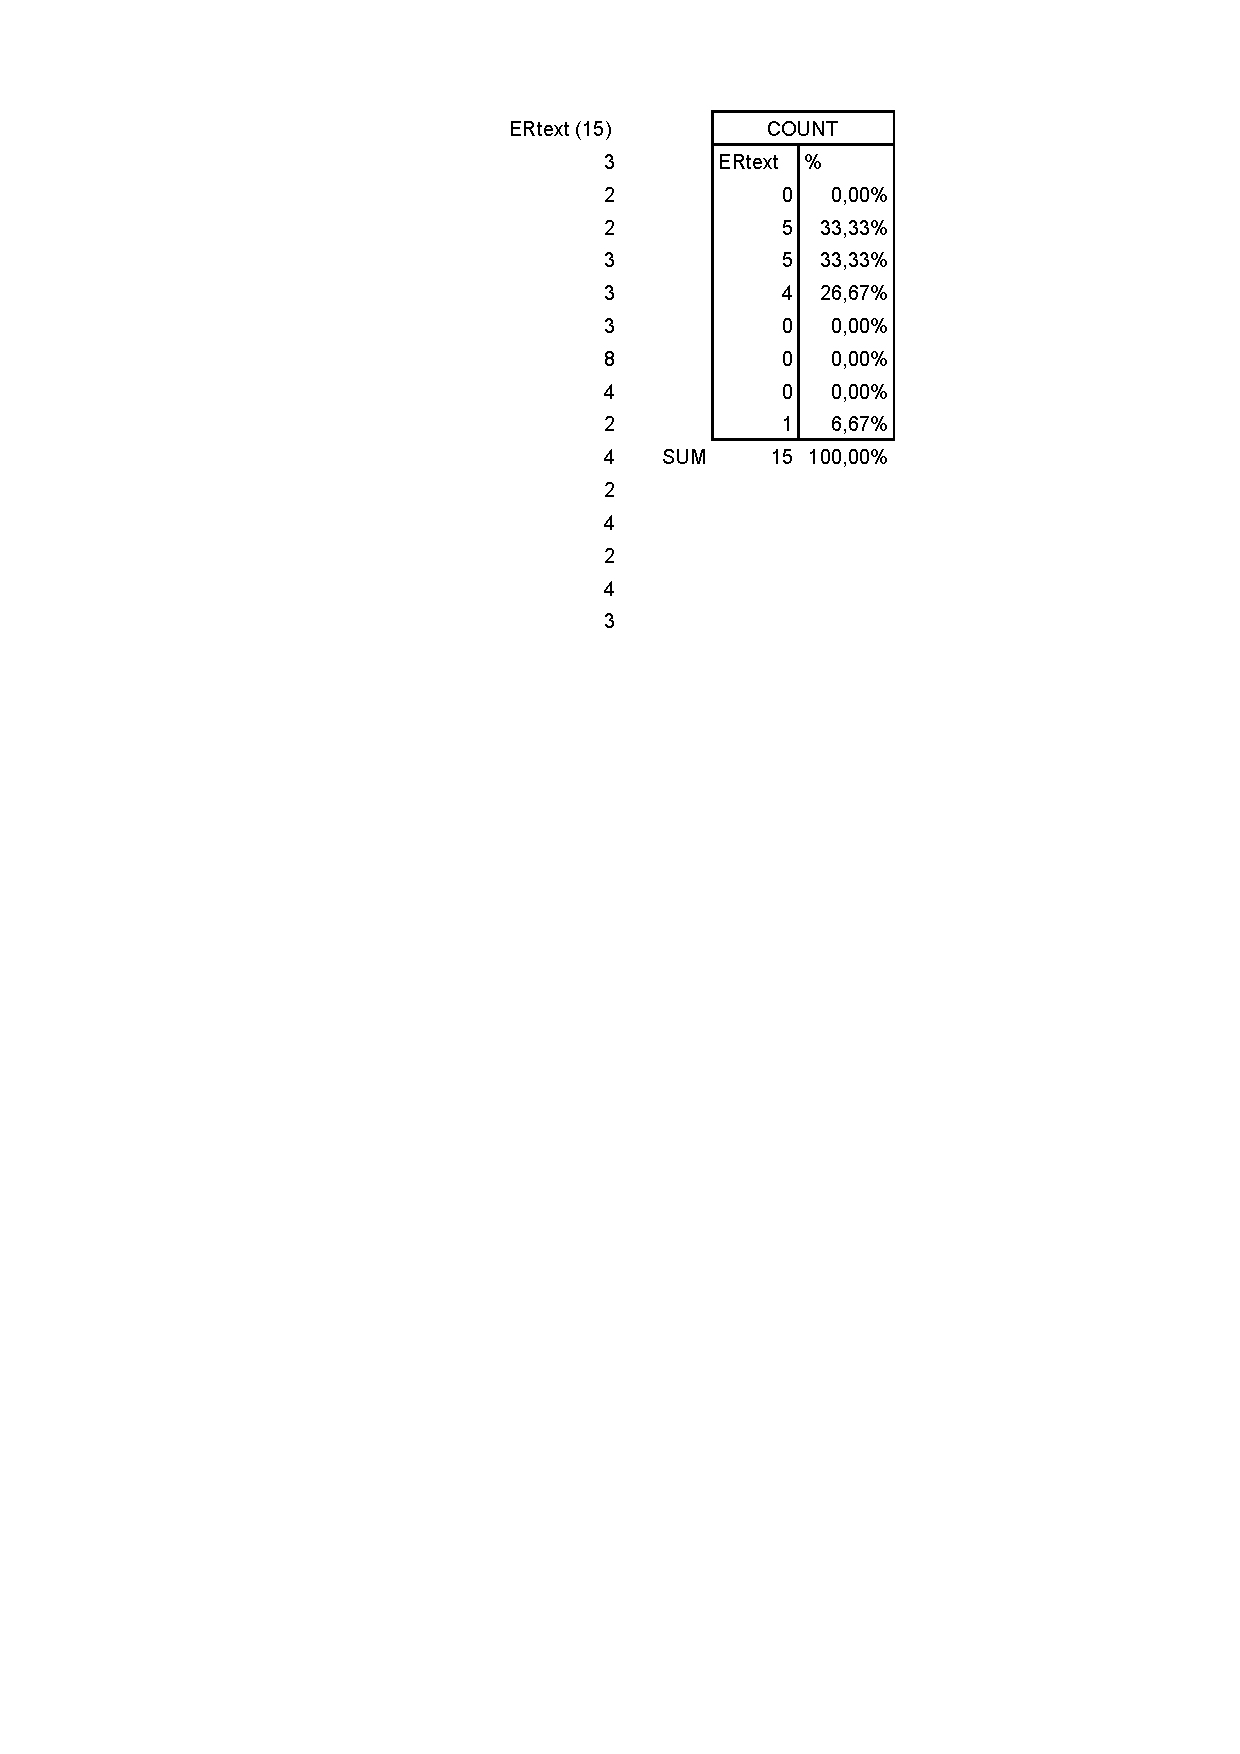
\includepdf[pages=-, frame=false, scale=0.70]{postextuais/appendix/EX3- Emocards-ERtext.pdf}
    % \caption{EX3 - Emocards - ERtext.}
    \label{fig:ex3EmocardsERtext}
\end{figure}

\newpage

\section{SUS - brModelo - EX3}

\begin{figure}[!htb]
    \centering
    % 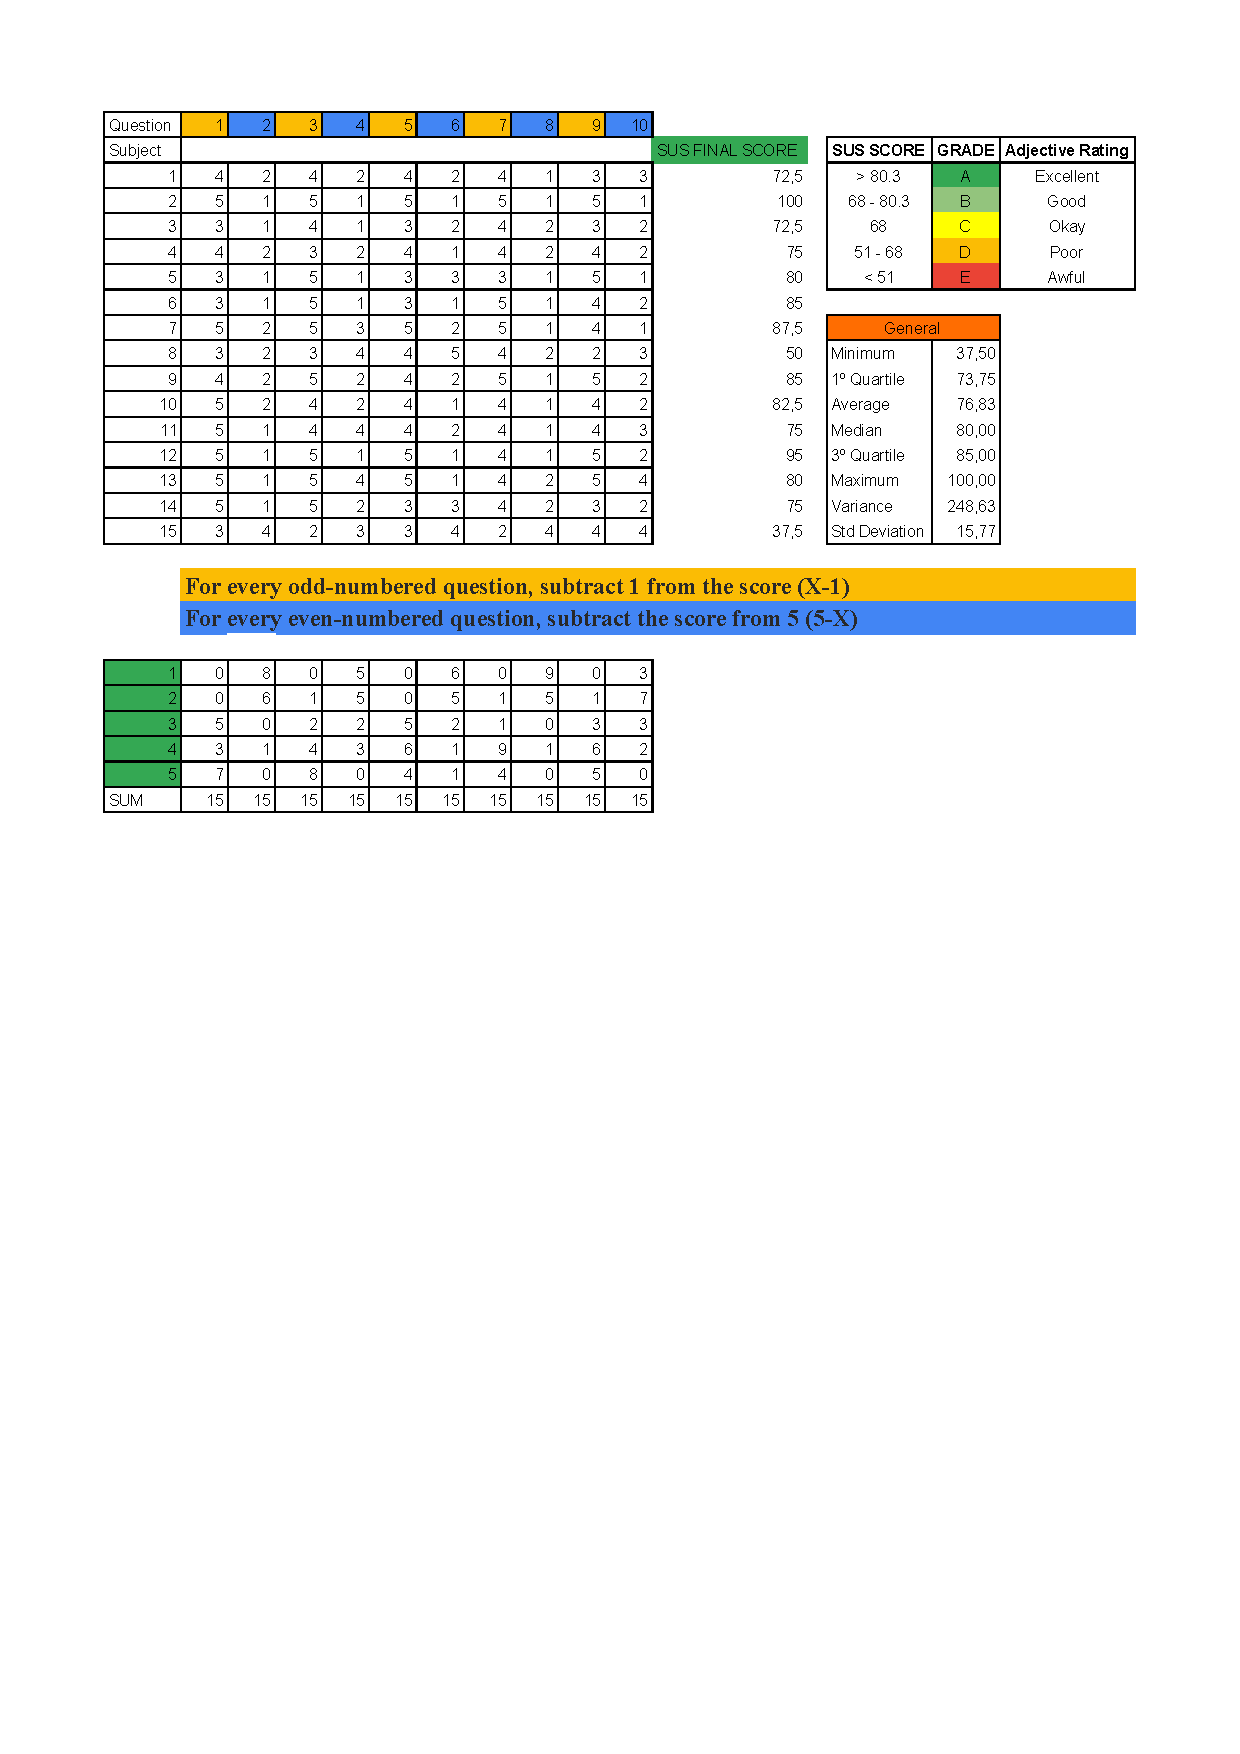
\includegraphics[]{postextuais/appendix/EX3-SUS-brModelo.pdf}
    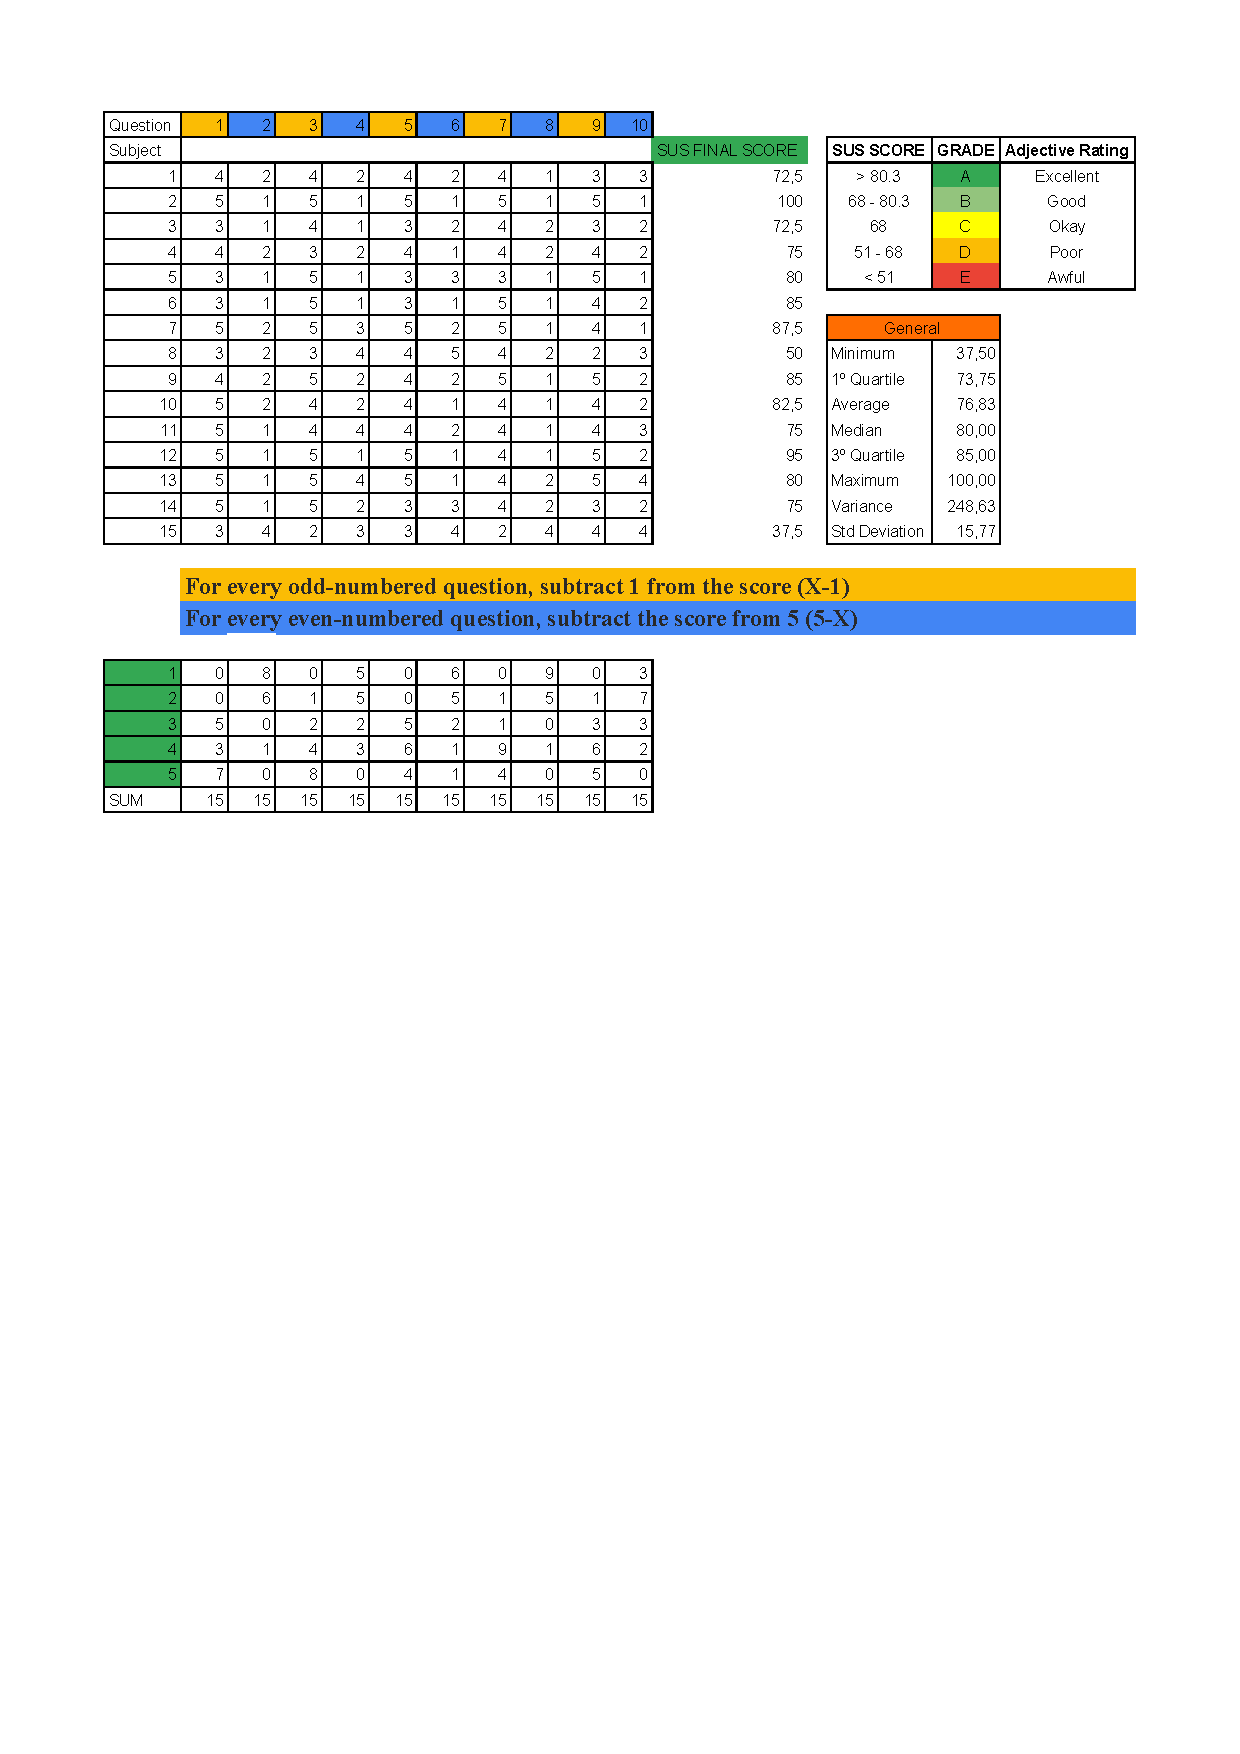
\includepdf[pages=-, frame=false, scale=0.80]{postextuais/appendix/EX3-SUS-brModelo.pdf}
    % \caption{EX3 - SUS - brModelo.}
    \label{fig:ex3EmocardsERtext}
\end{figure}

\newpage


\section{SUS - ERtext - EX3}

\begin{figure}[!htb]
    \centering
    % 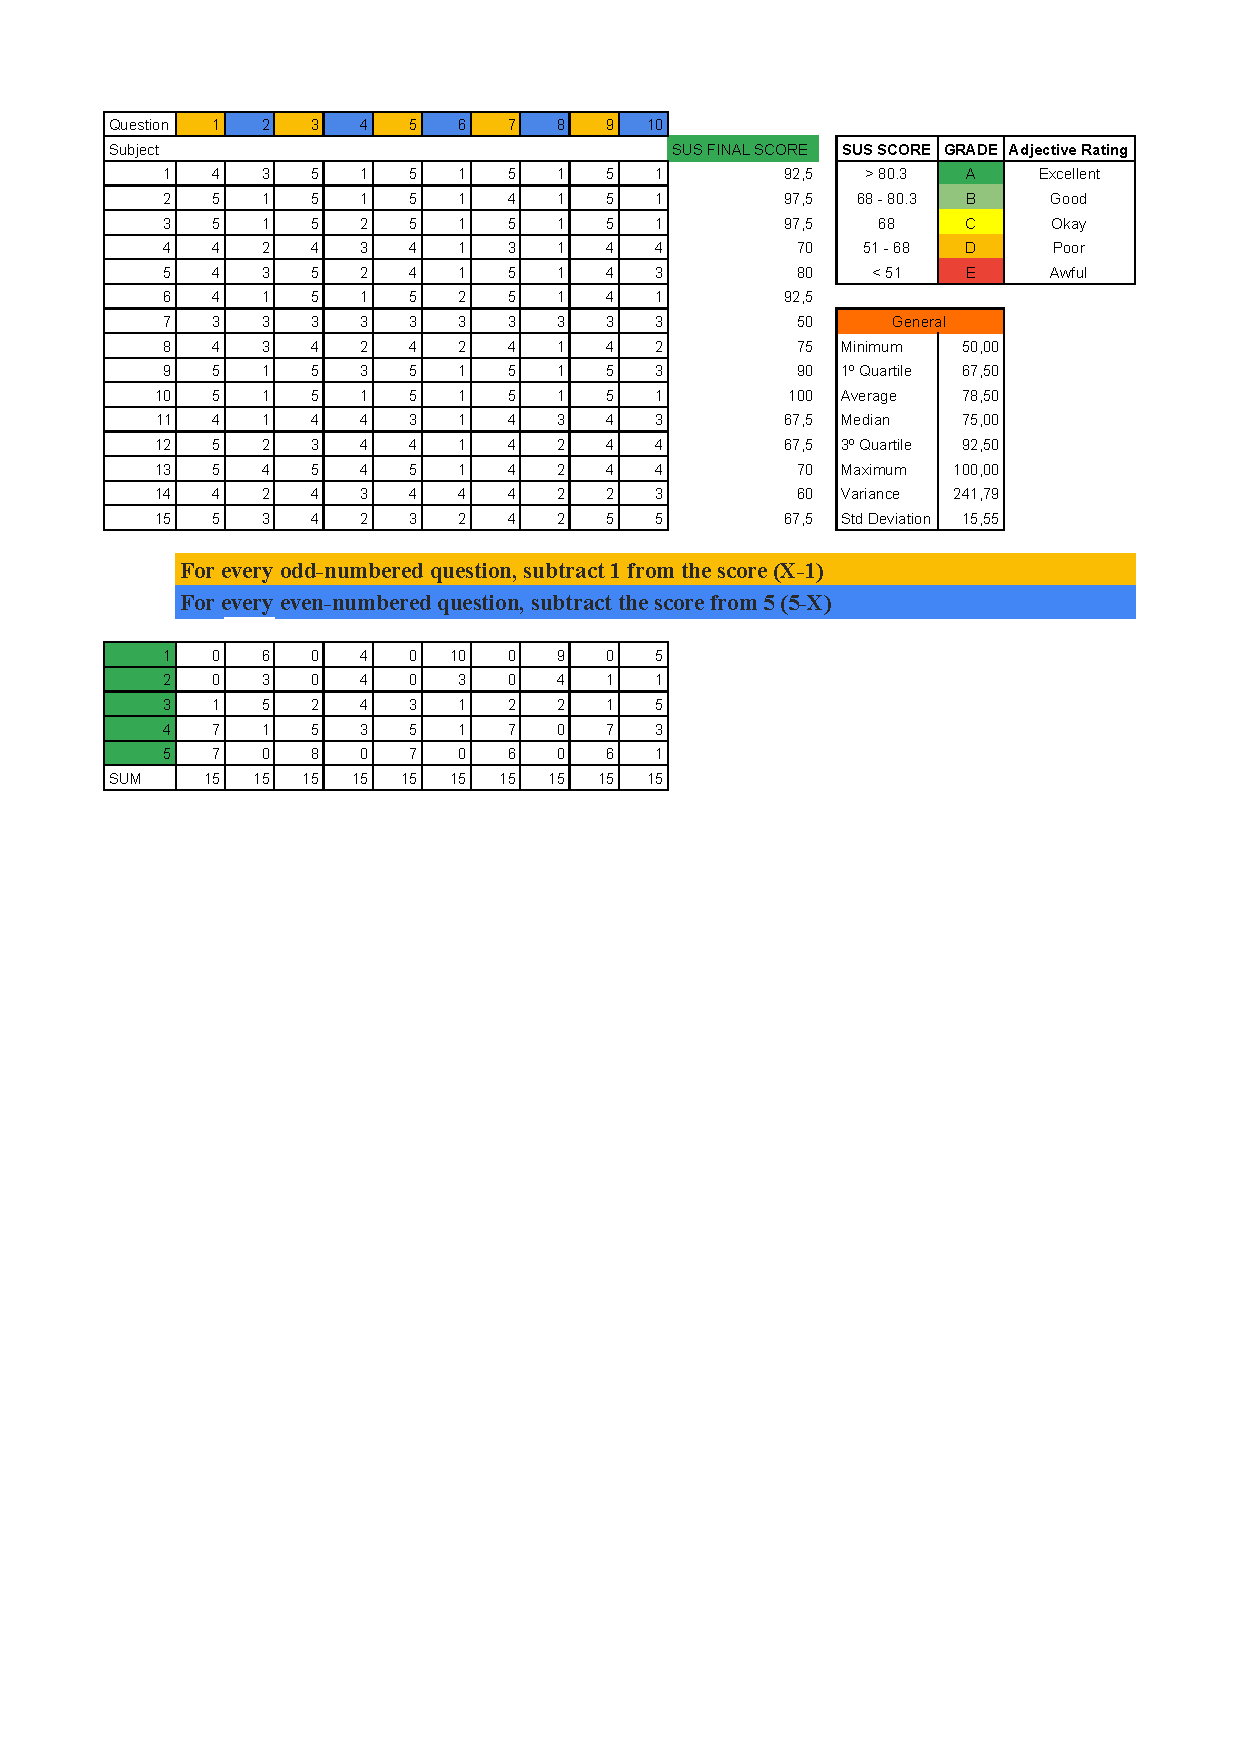
\includegraphics[]{postextuais/appendix/EX3-SUS-ERtext.pdf}
    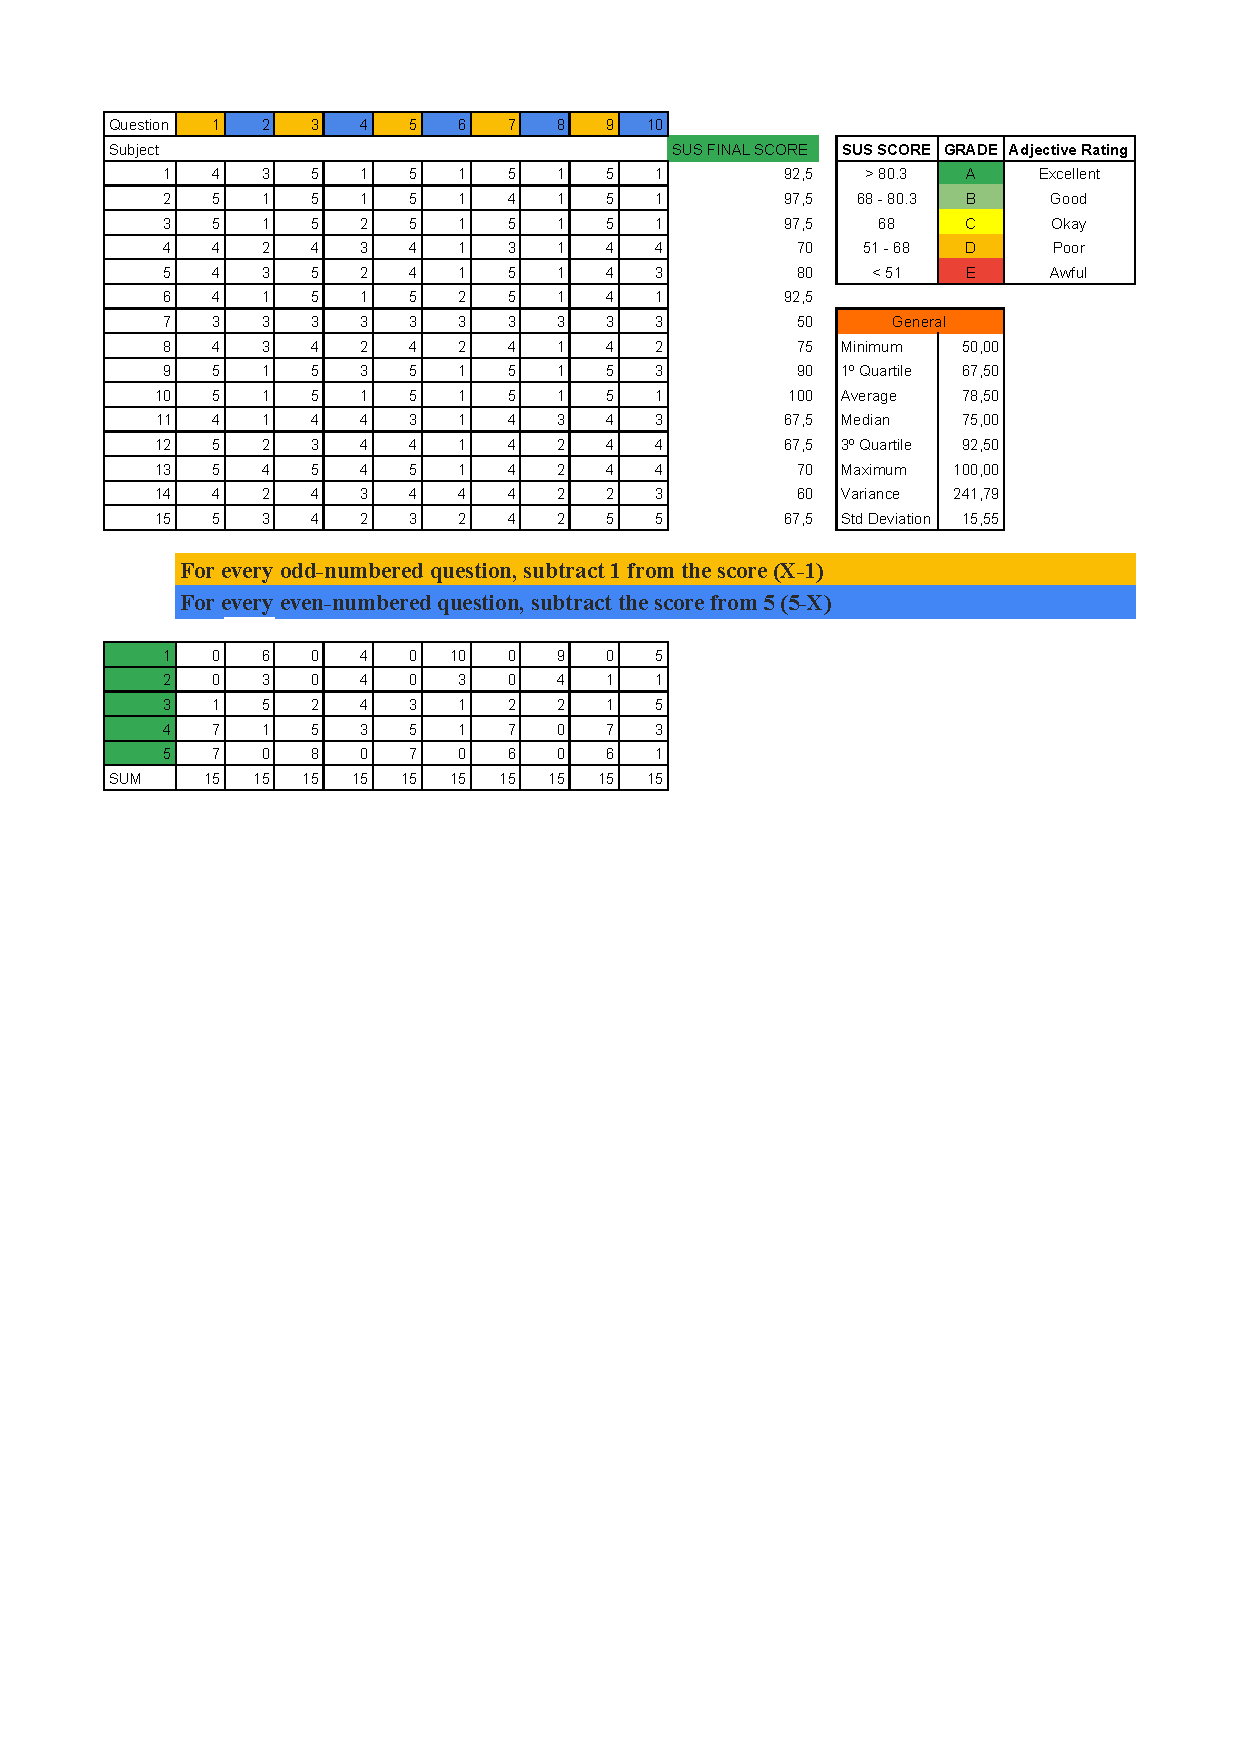
\includepdf[pages=-, frame=false, scale=0.80]{postextuais/appendix/EX3-SUS-ERtext.pdf}
    % \caption{EX3 - SUS - ERtext.}
    \label{fig:ex3EmocardsERtext}
\end{figure}

\end{apendicesenv}

% ==============================================================================
\chapter{Reference models and examples}\label{ap:referenceModels}
% ==============================================================================


\section{Instrument 1 (portuguese description)} \label{ap:Inst1Exp}

    \begin{figure}[!htb]
        \centering
        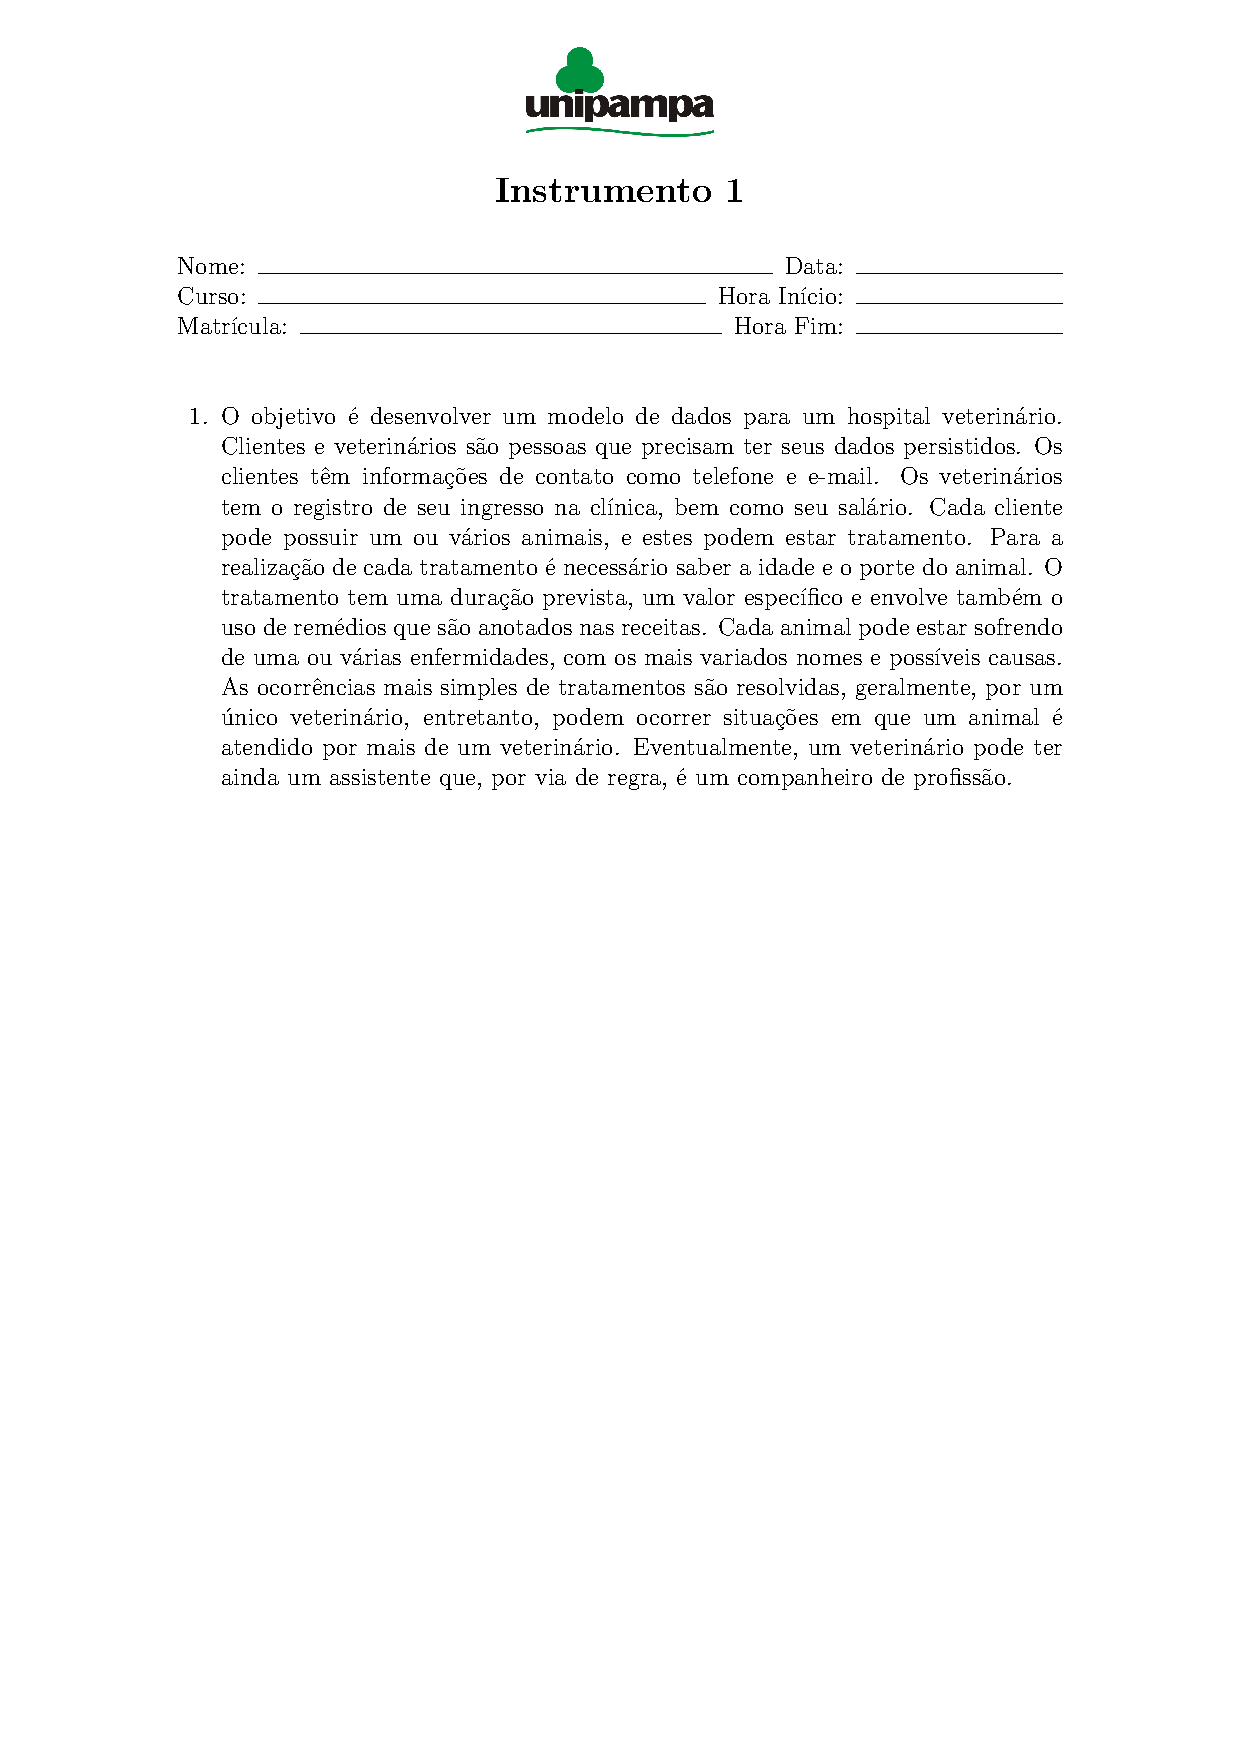
\includepdf[pages=-, frame=true, scale=0.65]{postextuais/appendix/Instrumento1.pdf} 
    \end{figure}

\newpage

\section{Instrument 2 (portuguese description)} \label{ap:Inst2Exp}

    \begin{figure}[!htb]
        \centering
        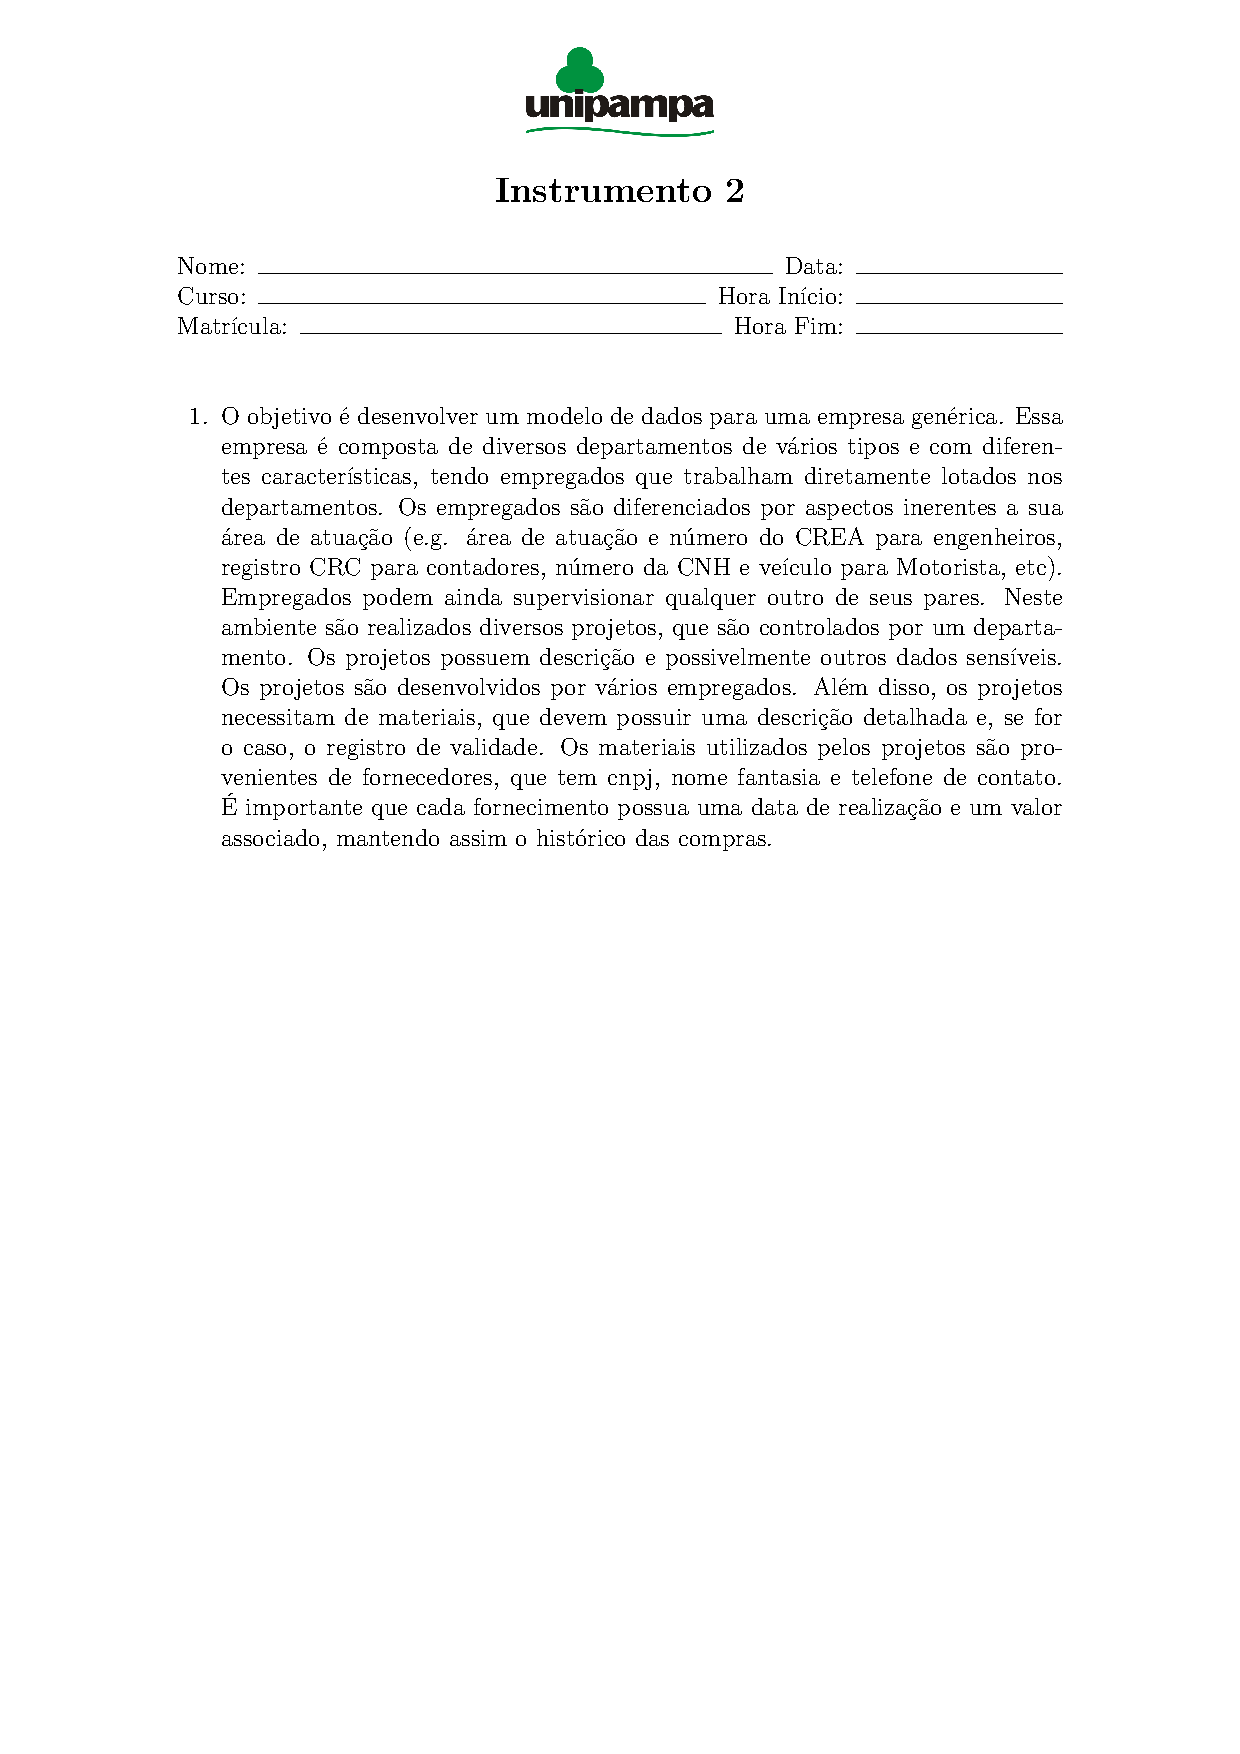
\includepdf[pages=-, frame=true, scale=0.65]{postextuais/appendix/Instrumento2.pdf} 
    \end{figure}

\newpage

\section{Reference model - brModelo (Instrument 1)}

\begin{figure}[!htb]
    \centering
    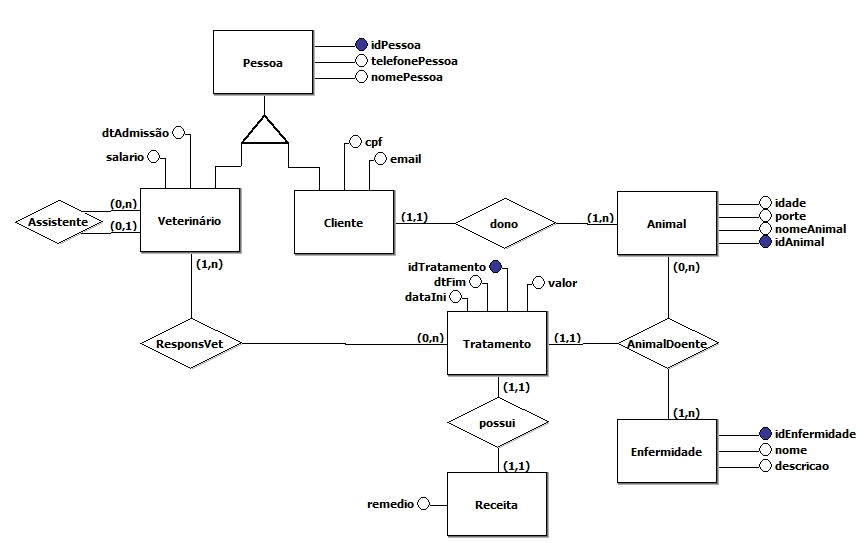
\includegraphics[scale=0.5]{postextuais/Instrument1 (brModelo Reference Model).jpg}
    % \caption{Caption}
    \label{fig:referenceModelbrModeloInst1}
\end{figure}

\newpage

\section{Reference model - brModelo (Instrument 2)}

\begin{figure}[!htb]
    \centering
    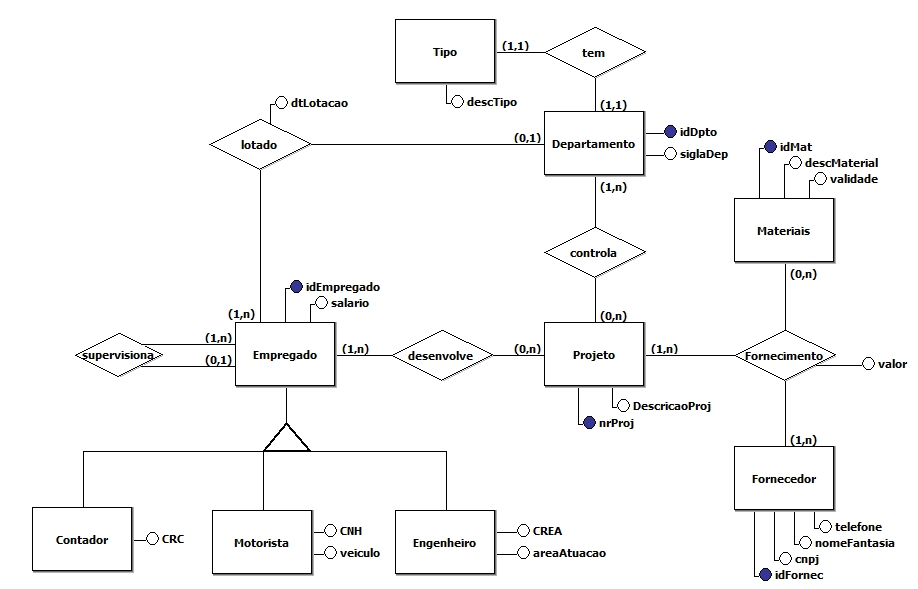
\includegraphics[scale=0.5]{postextuais/Instrument2 (brModelo Reference Model).jpg}
    % \caption{Caption}
    \label{fig:referenceModelbrModeloInst2}
\end{figure}

\newpage

\section{Reference model - ERtext (Instrument 1)}

\begin{figure}[!htb]
    \centering
    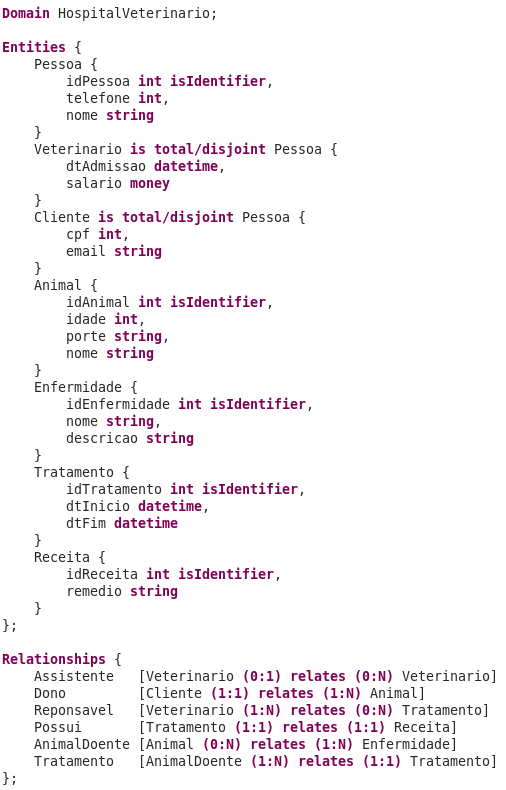
\includegraphics[scale=0.5]{postextuais/appendix/Instrument1-ReferenceModel-ERtext.png}
    % \caption{Caption}
    \label{fig:referenceModelERtextInst1}
\end{figure}

\newpage

\section{Reference model - ERtext (Instrument 2)}

\begin{figure}[!htb]
    \centering
    \includegraphics[scale=0.5]{postextuais/appendix/Instrument2-ReferenceModel-ERtext.png}
    % \caption{Caption}
    \label{fig:referenceModelERtextInst2}
\end{figure}

\newpage

\section{Modeled examples by a subject - brModelo}

\begin{figure}[!htb]
    \centering
    \includegraphics[scale=0.4]{postextuais/appendix/ExampleSubject-brModelo.png}
    % \caption{Caption}
    \label{fig:my_label}
\end{figure}

\newpage

\section{Modeled examples by a subject - ERtext}

\begin{figure}[!htb]
    \centering
    \includegraphics[scale=0.5]{postextuais/appendix/ExampleSubject-ERtext.png}
    % \caption{Caption}
    \label{fig:my_label}
\end{figure}

% -----------------------------------------------
% Anexos [OPCIONAL]
% -----------------------------------------------
%\begin{anexosenv}

% Imprime uma página indicando o início dos anexos
\partanexos

% Para cada anexo, um \chapter


%==============================================================================
%\chapter{Primeiro Anexo}
%==============================================================================



\end{anexosenv}


% -----------------------------------------------
% Índice Remissivo [OPCIONAL]
% -----------------------------------------------
% Veja o pacote makeindex para mais informações
\printindex


\end{document}
